% Options for packages loaded elsewhere
% Options for packages loaded elsewhere
\PassOptionsToPackage{unicode}{hyperref}
\PassOptionsToPackage{hyphens}{url}
%
\documentclass[
  ngerman,
  a4paper,
]{scrbook}
\usepackage{xcolor}
\usepackage{amsmath,amssymb}
\setcounter{secnumdepth}{5}
\usepackage{iftex}
\ifPDFTeX
  \usepackage[T1]{fontenc}
  \usepackage[utf8]{inputenc}
  \usepackage{textcomp} % provide euro and other symbols
\else % if luatex or xetex
  \usepackage{unicode-math} % this also loads fontspec
  \defaultfontfeatures{Scale=MatchLowercase}
  \defaultfontfeatures[\rmfamily]{Ligatures=TeX,Scale=1}
\fi
\usepackage{lmodern}
\ifPDFTeX\else
  % xetex/luatex font selection
\fi
% Use upquote if available, for straight quotes in verbatim environments
\IfFileExists{upquote.sty}{\usepackage{upquote}}{}
\IfFileExists{microtype.sty}{% use microtype if available
  \usepackage[]{microtype}
  \UseMicrotypeSet[protrusion]{basicmath} % disable protrusion for tt fonts
}{}
\makeatletter
\@ifundefined{KOMAClassName}{% if non-KOMA class
  \IfFileExists{parskip.sty}{%
    \usepackage{parskip}
  }{% else
    \setlength{\parindent}{0pt}
    \setlength{\parskip}{6pt plus 2pt minus 1pt}}
}{% if KOMA class
  \KOMAoptions{parskip=half}}
\makeatother
% Make \paragraph and \subparagraph free-standing
\makeatletter
\ifx\paragraph\undefined\else
  \let\oldparagraph\paragraph
  \renewcommand{\paragraph}{
    \@ifstar
      \xxxParagraphStar
      \xxxParagraphNoStar
  }
  \newcommand{\xxxParagraphStar}[1]{\oldparagraph*{#1}\mbox{}}
  \newcommand{\xxxParagraphNoStar}[1]{\oldparagraph{#1}\mbox{}}
\fi
\ifx\subparagraph\undefined\else
  \let\oldsubparagraph\subparagraph
  \renewcommand{\subparagraph}{
    \@ifstar
      \xxxSubParagraphStar
      \xxxSubParagraphNoStar
  }
  \newcommand{\xxxSubParagraphStar}[1]{\oldsubparagraph*{#1}\mbox{}}
  \newcommand{\xxxSubParagraphNoStar}[1]{\oldsubparagraph{#1}\mbox{}}
\fi
\makeatother


\usepackage{longtable,booktabs,array}
\newcounter{none} % for unnumbered tables
\usepackage{calc} % for calculating minipage widths
% Correct order of tables after \paragraph or \subparagraph
\usepackage{etoolbox}
\makeatletter
\patchcmd\longtable{\par}{\if@noskipsec\mbox{}\fi\par}{}{}
\makeatother
% Allow footnotes in longtable head/foot
\IfFileExists{footnotehyper.sty}{\usepackage{footnotehyper}}{\usepackage{footnote}}
\makesavenoteenv{longtable}
\usepackage{graphicx}
\makeatletter
\newsavebox\pandoc@box
\newcommand*\pandocbounded[1]{% scales image to fit in text height/width
  \sbox\pandoc@box{#1}%
  \Gscale@div\@tempa{\textheight}{\dimexpr\ht\pandoc@box+\dp\pandoc@box\relax}%
  \Gscale@div\@tempb{\linewidth}{\wd\pandoc@box}%
  \ifdim\@tempb\p@<\@tempa\p@\let\@tempa\@tempb\fi% select the smaller of both
  \ifdim\@tempa\p@<\p@\scalebox{\@tempa}{\usebox\pandoc@box}%
  \else\usebox{\pandoc@box}%
  \fi%
}
% Set default figure placement to htbp
\def\fps@figure{htbp}
\makeatother


% definitions for citeproc citations
\NewDocumentCommand\citeproctext{}{}
\NewDocumentCommand\citeproc{mm}{%
  \begingroup\def\citeproctext{#2}\cite{#1}\endgroup}
\makeatletter
 % allow citations to break across lines
 \let\@cite@ofmt\@firstofone
 % avoid brackets around text for \cite:
 \def\@biblabel#1{}
 \def\@cite#1#2{{#1\if@tempswa , #2\fi}}
\makeatother
\newlength{\cslhangindent}
\setlength{\cslhangindent}{1.5em}
\newlength{\csllabelwidth}
\setlength{\csllabelwidth}{3em}
\newenvironment{CSLReferences}[2] % #1 hanging-indent, #2 entry-spacing
 {\begin{list}{}{%
  \setlength{\itemindent}{0pt}
  \setlength{\leftmargin}{0pt}
  \setlength{\parsep}{0pt}
  % turn on hanging indent if param 1 is 1
  \ifodd #1
   \setlength{\leftmargin}{\cslhangindent}
   \setlength{\itemindent}{-1\cslhangindent}
  \fi
  % set entry spacing
  \setlength{\itemsep}{#2\baselineskip}}}
 {\end{list}}
\usepackage{calc}
\newcommand{\CSLBlock}[1]{\hfill\break\parbox[t]{\linewidth}{\strut\ignorespaces#1\strut}}
\newcommand{\CSLLeftMargin}[1]{\parbox[t]{\csllabelwidth}{\strut#1\strut}}
\newcommand{\CSLRightInline}[1]{\parbox[t]{\linewidth - \csllabelwidth}{\strut#1\strut}}
\newcommand{\CSLIndent}[1]{\hspace{\cslhangindent}#1}

\ifLuaTeX
\usepackage[bidi=basic,shorthands=off]{babel}
\else
\usepackage[bidi=default,shorthands=off]{babel}
\fi
\ifLuaTeX
  \usepackage{selnolig} % disable illegal ligatures
\fi


\setlength{\emergencystretch}{3em} % prevent overfull lines

\providecommand{\tightlist}{%
  \setlength{\itemsep}{0pt}\setlength{\parskip}{0pt}}



 


\usepackage{tabularx}
\usepackage{array}
\usepackage{etoolbox}
\usepackage{colortbl}
\usepackage{booktabs}
\usepackage{pdflscape}
\usepackage{fontspec}

% ---------------------------------------------------------
% Callouts
% ---------------------------------------------------------

\AtBeginDocument{
  \tcbset{
    fonttitle=\bfseries
  }
}

% ---------------------------------------------------------
% Tables
% ---------------------------------------------------------

% Gray zebra
\definecolor{zebrahead}{HTML}{E2E2E2}
\definecolor{zebralight}{HTML}{F8F8F8}
\definecolor{zebradark}{HTML}{EEEEEE}

% Blue zebra
\definecolor{zebrabluehead}{HTML}{D7E6F3}
\definecolor{zebrabluelight}{HTML}{F4F8FC}
\definecolor{zebrabluedark}{HTML}{E6F0F8}

% Table rule colors
\definecolor{tableline}{HTML}{D0D0D0}
\definecolor{tableheadrule}{HTML}{A8A8A8}
\definecolor{tableouterrule}{HTML}{B8B8B8}

% Thin, subtle rules
\setlength{\heavyrulewidth}{0.35pt}
\setlength{\lightrulewidth}{0.25pt}
\setlength{\cmidrulewidth}{0.25pt}

% No large booktabs gaps around rules
\setlength{\aboverulesep}{0pt}
\setlength{\belowrulesep}{0pt}

% ---------------------------------------------------------
% Font
% ---------------------------------------------------------

\setmainfont{Aptos}
\setsansfont{Aptos}
\makeatletter
\@ifpackageloaded{tcolorbox}{}{\usepackage[skins,breakable]{tcolorbox}}
\@ifpackageloaded{fontawesome5}{}{\usepackage{fontawesome5}}
\definecolor{quarto-callout-color}{HTML}{909090}
\definecolor{quarto-callout-note-color}{HTML}{0758E5}
\definecolor{quarto-callout-important-color}{HTML}{CC1914}
\definecolor{quarto-callout-warning-color}{HTML}{EB9113}
\definecolor{quarto-callout-tip-color}{HTML}{00A047}
\definecolor{quarto-callout-caution-color}{HTML}{FC5300}
\definecolor{quarto-callout-color-frame}{HTML}{acacac}
\definecolor{quarto-callout-note-color-frame}{HTML}{4582ec}
\definecolor{quarto-callout-important-color-frame}{HTML}{d9534f}
\definecolor{quarto-callout-warning-color-frame}{HTML}{f0ad4e}
\definecolor{quarto-callout-tip-color-frame}{HTML}{02b875}
\definecolor{quarto-callout-caution-color-frame}{HTML}{fd7e14}
\makeatother
\makeatletter
\@ifpackageloaded{bookmark}{}{\usepackage{bookmark}}
\makeatother
\makeatletter
\@ifpackageloaded{caption}{}{\usepackage{caption}}
\AtBeginDocument{%
\ifdefined\contentsname
  \renewcommand*\contentsname{Inhaltsverzeichnis}
\else
  \newcommand\contentsname{Inhaltsverzeichnis}
\fi
\ifdefined\listfigurename
  \renewcommand*\listfigurename{Abbildungsverzeichnis}
\else
  \newcommand\listfigurename{Abbildungsverzeichnis}
\fi
\ifdefined\listtablename
  \renewcommand*\listtablename{Tabellenverzeichnis}
\else
  \newcommand\listtablename{Tabellenverzeichnis}
\fi
\ifdefined\figurename
  \renewcommand*\figurename{Abbildung}
\else
  \newcommand\figurename{Abbildung}
\fi
\ifdefined\tablename
  \renewcommand*\tablename{Tabelle}
\else
  \newcommand\tablename{Tabelle}
\fi
}
\@ifpackageloaded{float}{}{\usepackage{float}}
\floatstyle{ruled}
\@ifundefined{c@chapter}{\newfloat{codelisting}{h}{lop}}{\newfloat{codelisting}{h}{lop}[chapter]}
\floatname{codelisting}{Listing}
\newcommand*\listoflistings{\listof{codelisting}{Listingverzeichnis}}
\makeatother
\makeatletter
\makeatother
\makeatletter
\@ifpackageloaded{caption}{}{\usepackage{caption}}
\@ifpackageloaded{subcaption}{}{\usepackage{subcaption}}
\makeatother
\usepackage{bookmark}
\IfFileExists{xurl.sty}{\usepackage{xurl}}{} % add URL line breaks if available
\urlstyle{same}
% fallback for those not using the hyperref driver hyperxmp:
\makeatletter
\@ifundefined{xmpquote}{\newcommand{\xmpquote}[1]{#1}}{}
\makeatother
\hypersetup{
  pdftitle={Magnetischen Maßverkörperungen für Weg- und Winkelmesssysteme},
  pdflang={de},
  hidelinks,
  pdfcreator={LaTeX via pandoc}}


\title{Magnetischen Maßverkörperungen für Weg- und Winkelmesssysteme}
\usepackage{etoolbox}
\makeatletter
\providecommand{\subtitle}[1]{% add subtitle to \maketitle
  \apptocmd{\@title}{\par {\large #1 \par}}{}{}
}
\makeatother
\subtitle{Terminologie, technische Darstellung, Einteilung, Messaufbau,
Vermessung und Bewertung}
\author{}
\date{}
\begin{document}
\frontmatter
\maketitle

\cleardoublepage
\thispagestyle{empty}

\textbf{Version}: 1.1

\textbf{Publikationsdatum}: 1. Oktober 2026

\textbf{DOI}: 10.5281/zenodo.XXXXXXX
\vspace{1.0cm}

\textbf{Autoren}: Michael Ortner, Rolf Slatter

\textbf{Herausgeber}: INNOMAG e.V., Ruhe Almend 8, 67655 Kaiserslautern
\vspace{1.0cm}

\textbf{Lizensiert} unter Creative Commons Namensnennung 4.0 International Lizenz (CC BY 4.0). Ausgenommen sind Inhalte Dritter, sofern diese nicht ausdrücklich anders gekennzeichnet sind.

Das Werk darf vervielfältigt, verbreitet, bearbeitet und für beliebige Zwecke, einschließlich kommerzieller Zwecke, verwendet werden, sofern eine angemessene Namensnennung erfolgt, auf die Lizenz verwiesen wird und Änderungen kenntlich gemacht werden.

\cleardoublepage

\renewcommand*\contentsname{Inhaltsverzeichnis}
{
\setcounter{tocdepth}{1}
\tableofcontents
}
\listoffigures
\listoftables

\mainmatter
\bookmarksetup{startatroot}

\chapter*{Mitwirkung und Autorschaft}\label{mitwirkung-und-autorschaft}
\addcontentsline{toc}{chapter}{Mitwirkung und Autorschaft}

\markboth{Mitwirkung und Autorschaft}{Mitwirkung und Autorschaft}

\section*{Mitwirkung}\label{mitwirkung}

\markright{Mitwirkung}

Diese Richtlinie bildet einen \textbf{gemeinsamen Rahmen} für die
Beschreibung, Darstellung und Bewertung magnetischer Maßverkörperungen
und soll unter Einbeziehung von Anwendern, Entwicklern und Fachleuten
kontinuierlich weiterentwickelt werden.

\textbf{Hinweise} auf Unklarheiten, Korrekturvorschläge, Ergänzungen und
Vorschläge zur Weiterentwicklung sind ausdrücklich willkommen.
Rückmeldungen können per E-Mail an
\href{mailto:guideline@innomag.org}{\textbf{guideline@innomag.org}}
gesendet oder über die Diskussionsmöglichkeiten im GitHub-Repository
\href{https://github.com/innomag-ev/Innomag-Guideline}{github.com/innomag-ev/Innomag-Guideline}
eingebracht werden.

\section*{Autoren}\label{autoren}

\markright{Autoren}

Verantwortung für die jeweiligen Kapitel; Entwicklung und Ausarbeitung
von Konzept, Struktur und Inhalten.

\begingroup
\footnotesize
\renewcommand{\baselinestretch}{1.12}\selectfont
\setlength{\tabcolsep}{5pt}
\setlength{\extrarowheight}{2.5pt}
\renewcommand{\arraystretch}{1.15}
{\def\LTcaptype{none} % do not increment counter
\begin{longtable*}[]{
  >{\raggedright\arraybackslash}p{(\linewidth - 4\tabcolsep) * \real{0.2000}}
  >{\raggedright\arraybackslash}p{(\linewidth - 4\tabcolsep) * \real{0.4000}}
  >{\raggedright\arraybackslash}p{(\linewidth - 4\tabcolsep) * \real{0.4000}}}
\arrayrulecolor{tableouterrule}
\toprule\noalign{}
\rowcolor{zebrahead}
\begin{minipage}[b]{\linewidth}\raggedright
\textbf{Name}
\end{minipage} & \begin{minipage}[b]{\linewidth}\raggedright
\textbf{Organisation}
\end{minipage} & \begin{minipage}[b]{\linewidth}\raggedright
\textbf{Beitrag}
\end{minipage} \\
\arrayrulecolor{tableheadrule}
\specialrule{0.35pt}{0pt}{0pt}
\endhead
\arrayrulecolor{tableouterrule}
\specialrule{0.30pt}{0pt}{0pt}
\endlastfoot
\rowcolor{zebralight}
Michael Ortner & Silicon Austria Labs GmbH & Kapitel 2--8, Editor \\
\arrayrulecolor{tableline}
\specialrule{0.15pt}{0pt}{0pt}
\rowcolor{zebradark}
Rolf Slatter & INNOMAG e. V. & Kapitel 1 \\
\arrayrulecolor{tableline}
\specialrule{0.15pt}{0pt}{0pt}
\end{longtable*}
}
\endgroup

\section*{Fachliche Mitwirkung}\label{fachliche-mitwirkung}

\markright{Fachliche Mitwirkung}

Fachlicher Austausch und Diskussion; fachliche Beiträge zu einzelnen
Kapiteln; Rückmeldungen zu Inhalten; Review ausgewählter Abschnitte;
Begleitung der konzeptionellen Weiterentwicklung.

\begingroup
\footnotesize
\renewcommand{\baselinestretch}{1.12}\selectfont
\setlength{\tabcolsep}{5pt}
\setlength{\extrarowheight}{2.5pt}
\renewcommand{\arraystretch}{1.15}
{\def\LTcaptype{none} % do not increment counter
\begin{longtable*}[]{
  >{\raggedright\arraybackslash}p{(\linewidth - 4\tabcolsep) * \real{0.2000}}
  >{\raggedright\arraybackslash}p{(\linewidth - 4\tabcolsep) * \real{0.4000}}
  >{\raggedright\arraybackslash}p{(\linewidth - 4\tabcolsep) * \real{0.4000}}}
\arrayrulecolor{tableouterrule}
\toprule\noalign{}
\rowcolor{zebrahead}
\begin{minipage}[b]{\linewidth}\raggedright
\textbf{Name}
\end{minipage} & \begin{minipage}[b]{\linewidth}\raggedright
\textbf{Organisation}
\end{minipage} & \begin{minipage}[b]{\linewidth}\raggedright
\textbf{Beitrag}
\end{minipage} \\
\arrayrulecolor{tableheadrule}
\specialrule{0.35pt}{0pt}{0pt}
\endhead
\arrayrulecolor{tableouterrule}
\specialrule{0.30pt}{0pt}{0pt}
\endlastfoot
\rowcolor{zebralight}
Armin Pfeffer & Bogen Magnetics GmbH & Fachliche Mitwirkung \\
\arrayrulecolor{tableline}
\specialrule{0.15pt}{0pt}{0pt}
\rowcolor{zebradark}
Axel Bartos & TE Connectivity & Fachliche Mitwirkung \\
\arrayrulecolor{tableline}
\specialrule{0.15pt}{0pt}{0pt}
\rowcolor{zebralight}
Benjamin Wenzel & Matesy GmbH & Fachliche Mitwirkung \\
\arrayrulecolor{tableline}
\specialrule{0.15pt}{0pt}{0pt}
\rowcolor{zebradark}
Bernd Böhle & ELSOMA GmbH & Fachliche Mitwirkung \\
\arrayrulecolor{tableline}
\specialrule{0.15pt}{0pt}{0pt}
\rowcolor{zebralight}
Florian Slanovc & Silicon Austria Labs GmbH & Fachliche Mitwirkung \\
\arrayrulecolor{tableline}
\specialrule{0.15pt}{0pt}{0pt}
\rowcolor{zebradark}
Heiko Knoll & ITK Precisioning GmbH & Fachliche Mitwirkung \\
\arrayrulecolor{tableline}
\specialrule{0.15pt}{0pt}{0pt}
\rowcolor{zebralight}
Jürgen Gerber & INNOMAG e.V. & Fachliche Mitwirkung; Koordination \\
\arrayrulecolor{tableline}
\specialrule{0.15pt}{0pt}{0pt}
\rowcolor{zebradark}
Magnus Meier & IC-Haus GmbH & Fachliche Mitwirkung \\
\arrayrulecolor{tableline}
\specialrule{0.15pt}{0pt}{0pt}
\rowcolor{zebralight}
Mattias Pelkner & Bundesanstalt für Materialforschung und -prüfung &
Fachliche Mitwirkung \\
\arrayrulecolor{tableline}
\specialrule{0.15pt}{0pt}{0pt}
\rowcolor{zebradark}
Michael Melzer & Bundesanstalt für Materialforschung und -prüfung &
Fachliche Mitwirkung \\
\arrayrulecolor{tableline}
\specialrule{0.15pt}{0pt}{0pt}
\rowcolor{zebralight}
Michal Pham & Baumer Group & Fachliche Mitwirkung \\
\arrayrulecolor{tableline}
\specialrule{0.15pt}{0pt}{0pt}
\rowcolor{zebradark}
Pascal Hille & Sensitec GmbH & Fachliche Mitwirkung; Beitrag zu Kapitel
2 \\
\arrayrulecolor{tableline}
\specialrule{0.15pt}{0pt}{0pt}
\rowcolor{zebralight}
Phillip Beran & Fraunhofer Institut für Integrierte Schaltungen IIS &
Fachliche Mitwirkung \\
\arrayrulecolor{tableline}
\specialrule{0.15pt}{0pt}{0pt}
\rowcolor{zebradark}
Ralph Bauer & Balluff GmbH & Fachliche Mitwirkung \\
\arrayrulecolor{tableline}
\specialrule{0.15pt}{0pt}{0pt}
\rowcolor{zebralight}
René Buß & Sensitec GmbH & Fachliche Mitwirkung \\
\arrayrulecolor{tableline}
\specialrule{0.15pt}{0pt}{0pt}
\rowcolor{zebradark}
Rocco Holzhey & Innovent GmbH & Fachliche Mitwirkung \\
\arrayrulecolor{tableline}
\specialrule{0.15pt}{0pt}{0pt}
\rowcolor{zebralight}
Sebastian Rivera & ITK Precisioning GmbH & Fachliche Mitwirkung \\
\arrayrulecolor{tableline}
\specialrule{0.15pt}{0pt}{0pt}
\rowcolor{zebradark}
Sibylle Sievers & Physikalisch-Technische Bundesanstalt & Fachliche
Mitwirkung \\
\arrayrulecolor{tableline}
\specialrule{0.15pt}{0pt}{0pt}
\rowcolor{zebralight}
Stefan Herzog & ZF Friedrichshafen AG & Fachliche Mitwirkung; Beitrag zu
Kapitel 2 \\
\arrayrulecolor{tableline}
\specialrule{0.15pt}{0pt}{0pt}
\rowcolor{zebradark}
Thomas Schliesch & Max Baermann GmbH & Fachliche Mitwirkung \\
\arrayrulecolor{tableline}
\specialrule{0.15pt}{0pt}{0pt}
\rowcolor{zebralight}
Werner Pessenhofer & Nanomag GmbH & Fachliche Mitwirkung \\
\arrayrulecolor{tableline}
\specialrule{0.15pt}{0pt}{0pt}
\end{longtable*}
}
\endgroup

\bookmarksetup{startatroot}

\chapter*{Vorwort}\label{vorwort}
\addcontentsline{toc}{chapter}{Vorwort}

\markboth{Vorwort}{Vorwort}

Magnetische Weg- und Winkelmesssysteme sind aus der modernen
Automatisierungs-, Antriebs- und Fahrzeugtechnik nicht mehr wegzudenken.
Ihr Herzstück -- die magnetische Maßverkörperung -- wird jedoch über die
gesamte Wertschöpfungskette hinweg von sehr unterschiedlichen Akteuren
entwickelt, gefertigt, magnetisiert und geprüft. Gerade an diesen
Schnittstellen zeigt sich immer wieder, wie sehr eine gemeinsame,
eindeutige Sprache fehlt.

Einen ersten wichtigen Schritt zur Abhilfe stellte die DIN SPEC 91411
(Innomag 2022) dar. Die praktische Arbeit mit dieser Spezifikation in
den vergangenen Jahren hat den Wert einer einheitlichen Beschreibung
eindrücklich bestätigt -- zugleich aber gezeigt, dass einige zentrale
Begriffe in der täglichen Anwendung unterschiedlich verstanden und
ausgelegt wurden. Aus diesem Erfahrungsschatz heraus entstand der
Wunsch, bestehende Definitionen zu schärfen, Lücken zu schließen und die
Darstellungsregeln konsistent auf physikalische Grundlagen
zurückzuführen.

Die vorliegende Richtlinie ist das Ergebnis dieser Weiterentwicklung.
Sie wurde von einem Konsortium aus Mitgliedsfirmen und -instituten des
INNOMAG e. V. erarbeitet, dass Hersteller, Anwender und
Forschungseinrichtungen an einen Tisch gebracht hat. In dieser
Zusammensetzung spiegelt das Dokument die geballte Praxiserfahrung der
Fachgemeinschaft wider und verfolgt ein klares Ziel: eine gemeinsame,
allgemein verständliche Terminologie für magnetische Maßverkörperungen
zu etablieren, die Missverständnisse vermeidet und den fachlichen
Austausch über Unternehmens- und Ländergrenzen hinweg erleichtert.

Ein besonderer Dank gilt Herrn Dr.~Michael Ortner von den Silicon
Austria Labs, der sich in maßgeblicher Weise an der Erstellung dieser
Richtlinie beteiligt hat. Ebenso danken wir allen mitwirkenden
Autorinnen und Autoren sowie den beteiligten Unternehmen und Instituten,
ohne deren Engagement dieses Dokument nicht möglich gewesen wäre.

Wir wünschen allen Leserinnen und Lesern eine anregende Lektüre und
hoffen, dass diese Richtlinie in der Praxis ebenso breite Anwendung
findet wie ihre Vorgängerin.

Dr.~Rolf Slatter, Vorstandsvorsitzender, INNOMAG e. V.

Dr.~Jürgen Gerber, Geschäftsführer, INNOMAG e. V.

\bookmarksetup{startatroot}

\chapter*{Abkürzungen und
Formelzeichen}\label{abkuxfcrzungen-und-formelzeichen}
\addcontentsline{toc}{chapter}{Abkürzungen und Formelzeichen}

\markboth{Abkürzungen und Formelzeichen}{Abkürzungen und Formelzeichen}

\section*{Abkürzungsverzeichnis}\label{abkuxfcrzungsverzeichnis}

\markright{Abkürzungsverzeichnis}

\begingroup
\footnotesize
\renewcommand{\baselinestretch}{1.12}\selectfont
\setlength{\tabcolsep}{5pt}
\setlength{\extrarowheight}{2.5pt}
\renewcommand{\arraystretch}{1.15}
{\def\LTcaptype{none} % do not increment counter
\begin{longtable*}[]{
  >{\raggedright\arraybackslash}p{(\linewidth - 2\tabcolsep) * \real{0.2000}}
  >{\raggedright\arraybackslash}p{(\linewidth - 2\tabcolsep) * \real{0.8000}}}
\arrayrulecolor{tableouterrule}
\toprule\noalign{}
\rowcolor{zebrahead}
\begin{minipage}[b]{\linewidth}\raggedright
\textbf{Abkürzung}
\end{minipage} & \begin{minipage}[b]{\linewidth}\raggedright
\textbf{Bedeutung}
\end{minipage} \\
\arrayrulecolor{tableheadrule}
\specialrule{0.35pt}{0pt}{0pt}
\endhead
\arrayrulecolor{tableouterrule}
\specialrule{0.30pt}{0pt}{0pt}
\endlastfoot
\rowcolor{zebralight}
KS & Koordinatensystem \\
\arrayrulecolor{tableline}
\specialrule{0.15pt}{0pt}{0pt}
\rowcolor{zebradark}
IP & in-plane \\
\arrayrulecolor{tableline}
\specialrule{0.15pt}{0pt}{0pt}
\rowcolor{zebralight}
OOP & out-of-plane \\
\arrayrulecolor{tableline}
\specialrule{0.15pt}{0pt}{0pt}
\end{longtable*}
}
\endgroup

\section*{Symbolverzeichnis grundlegender
Größen}\label{symbolverzeichnis-grundlegender-gruxf6uxdfen}

\markright{Symbolverzeichnis grundlegender Größen}

\begingroup
\footnotesize
\renewcommand{\baselinestretch}{1.12}\selectfont
\setlength{\tabcolsep}{5pt}
\setlength{\extrarowheight}{2.5pt}
\renewcommand{\arraystretch}{1.15}
{\def\LTcaptype{none} % do not increment counter
\begin{longtable*}[]{
  >{\raggedright\arraybackslash}p{(\linewidth - 4\tabcolsep) * \real{0.2000}}
  >{\raggedright\arraybackslash}p{(\linewidth - 4\tabcolsep) * \real{0.6000}}
  >{\raggedright\arraybackslash}p{(\linewidth - 4\tabcolsep) * \real{0.2000}}}
\arrayrulecolor{tableouterrule}
\toprule\noalign{}
\rowcolor{zebrahead}
\begin{minipage}[b]{\linewidth}\raggedright
\textbf{Symbol}
\end{minipage} & \begin{minipage}[b]{\linewidth}\raggedright
\textbf{Bedeutung}
\end{minipage} & \begin{minipage}[b]{\linewidth}\raggedright
\textbf{Einheit}
\end{minipage} \\
\arrayrulecolor{tableheadrule}
\specialrule{0.35pt}{0pt}{0pt}
\endhead
\arrayrulecolor{tableouterrule}
\specialrule{0.30pt}{0pt}{0pt}
\endlastfoot
\rowcolor{zebralight}
\(\vec{B}\) & magnetische Flussdichte, B-Feld & T \\
\arrayrulecolor{tableline}
\specialrule{0.15pt}{0pt}{0pt}
\rowcolor{zebradark}
\(\vec{H}\) & magnetische Feldstärke, H-Feld & A/m \\
\arrayrulecolor{tableline}
\specialrule{0.15pt}{0pt}{0pt}
\rowcolor{zebralight}
\(\vec{M}\) & Magnetisierung & A/m \\
\arrayrulecolor{tableline}
\specialrule{0.15pt}{0pt}{0pt}
\rowcolor{zebradark}
\(\vec{J}\) & magnetische Polarisation & T \\
\arrayrulecolor{tableline}
\specialrule{0.15pt}{0pt}{0pt}
\rowcolor{zebralight}
\(\mu_0\) & Vakuumpermeabilität & T m/A \\
\arrayrulecolor{tableline}
\specialrule{0.15pt}{0pt}{0pt}
\rowcolor{zebradark}
\(p\) & Koordinate in Längsrichtung & m bzw. ° \\
\arrayrulecolor{tableline}
\specialrule{0.15pt}{0pt}{0pt}
\rowcolor{zebralight}
\(o\) & Koordinate in Querrichtung & m \\
\arrayrulecolor{tableline}
\specialrule{0.15pt}{0pt}{0pt}
\rowcolor{zebradark}
\(n\) & Koordinate in Abstandsrichtung; Messhöhe bei entsprechender
Verwendung & m \\
\arrayrulecolor{tableline}
\specialrule{0.15pt}{0pt}{0pt}
\rowcolor{zebralight}
\(o\) & Ursprung eines Koordinatensystems & -- \\
\arrayrulecolor{tableline}
\specialrule{0.15pt}{0pt}{0pt}
\rowcolor{zebradark}
\(\vec{e}_p\) & Einheitsvektor in \(p\)-Richtung & -- \\
\arrayrulecolor{tableline}
\specialrule{0.15pt}{0pt}{0pt}
\rowcolor{zebralight}
\(\vec{e}_o\) & Einheitsvektor in \(o\)-Richtung & -- \\
\arrayrulecolor{tableline}
\specialrule{0.15pt}{0pt}{0pt}
\rowcolor{zebradark}
\(\vec{e}_n\) & Einheitsvektor in \(n\)-Richtung & -- \\
\arrayrulecolor{tableline}
\specialrule{0.15pt}{0pt}{0pt}
\rowcolor{zebralight}
\(\vec{r}\) & Orts- bzw. Lagevektor & m \\
\arrayrulecolor{tableline}
\specialrule{0.15pt}{0pt}{0pt}
\end{longtable*}
}
\endgroup

\bookmarksetup{startatroot}

\chapter{Einleitung}\label{einleitung}

\section{Hintergrund und Zielsetzung}\label{hintergrund-und-zielsetzung}

\textbf{Magnetische Weg- und Winkelmesssysteme} erfassen die
Relativposition zweier Bauteile entlang einer festgelegten
Bewegungskoordinate. Bei Wegmesssystemen wird diese als Weg entlang
eines Pfads, bei Winkelmesssystemen als Drehwinkel um eine mechanische
Achse angegeben. Sie machen einen großen Teil der magnetischen
Positionsmesssysteme in industriellen Anwendungen aus.

Typischerweise bestehen magnetische Weg- und Winkelmesssysteme aus einem
felderzeugenden Dauermagneten -- der \textbf{magnetischen
Maßverkörperung} -- und einem \textbf{magnetischen Sensor}. Der Sensor
erfasst das von der Maßverkörperung erzeugte Magnetfeld und wandelt die
darin enthaltene Positionsinformation in elektrische Ausgangssignale um.
Aus diesen Signalen wird die relative Position zwischen Sensor und
Maßverkörperung bestimmt.

\begin{tcolorbox}[enhanced jigsaw, arc=.35mm, bottomrule=.15mm, bottomtitle=1mm, breakable, colback=white, colbacktitle=quarto-callout-tip-color!10!white, colframe=quarto-callout-tip-color-frame, coltitle=black, left=2mm, leftrule=.75mm, opacityback=0, opacitybacktitle=0.6, rightrule=.15mm, title=\textcolor{quarto-callout-tip-color}{\faLightbulb}\hspace{0.5em}{Hinweis}, titlerule=0mm, toprule=.15mm, toptitle=1mm]

\emph{Der Begriff \textbf{Sensor} wird in der Praxis uneinheitlich für
Sensorelemente als Wandlerelemente und für Sensormodule als funktionale
Gesamteinheiten verwendet. In dieser Richtlinie wird er eingesetzt, wenn
eine genaue Unterscheidung nicht erforderlich ist.}

\end{tcolorbox}

Das berührungslose magnetische Messprinzip bietet \textbf{Vorteile}
hinsichtlich Robustheit, Verschleißfreiheit,
Verschmutzungsunempfindlichkeit, Integrationsfähigkeit und Kosten und
hat sich daher in zahlreichen industriellen Anwendungen etabliert.
(Cassing u.~a. 2018; Michalowsky und Schneider 2006; Schwegler und Rapp
2016; Hilzinger und Rodewald 2013; Coey 2010; Cullity und Graham 2008)

Zur \textbf{Herstellung} magnetischer Maßverkörperungen werden Rohlinge
in einem Magnetisierungsprozess magnetisch codiert. Die Auswahl von
Material und Geometrie der Rohlinge richtet sich nach den Anforderungen
der späteren Anwendung sowie nach der Komplexität der erforderlichen
magnetischen Codierung. Diese reicht von einfachen homogenen
Magnetisierungen bis hin zu komplexen Mustern. Materialinhomogenitäten
sowie mechanische Toleranzen bei Formgebung, Magnetisierung und Montage
zählen dabei zu den \textbf{qualitätsrelevanten Fehlerquellen}
(Schliesch 2022) und können die Güte des gesamten Messsystems in der
Endanwendung maßgeblich beeinflussen (Kolb u.~a. 2019).

Herstellung und Prüfung magnetischer Maßverkörperungen bilden einen
wesentlichen Abschnitt der Wertschöpfungskette „Vom Rohstoff bis zur
Anwendung``, die in Abbildung~\ref{fig-sec01-value_chain} dargestellt
ist.

\begin{figure}[h]

\centering{

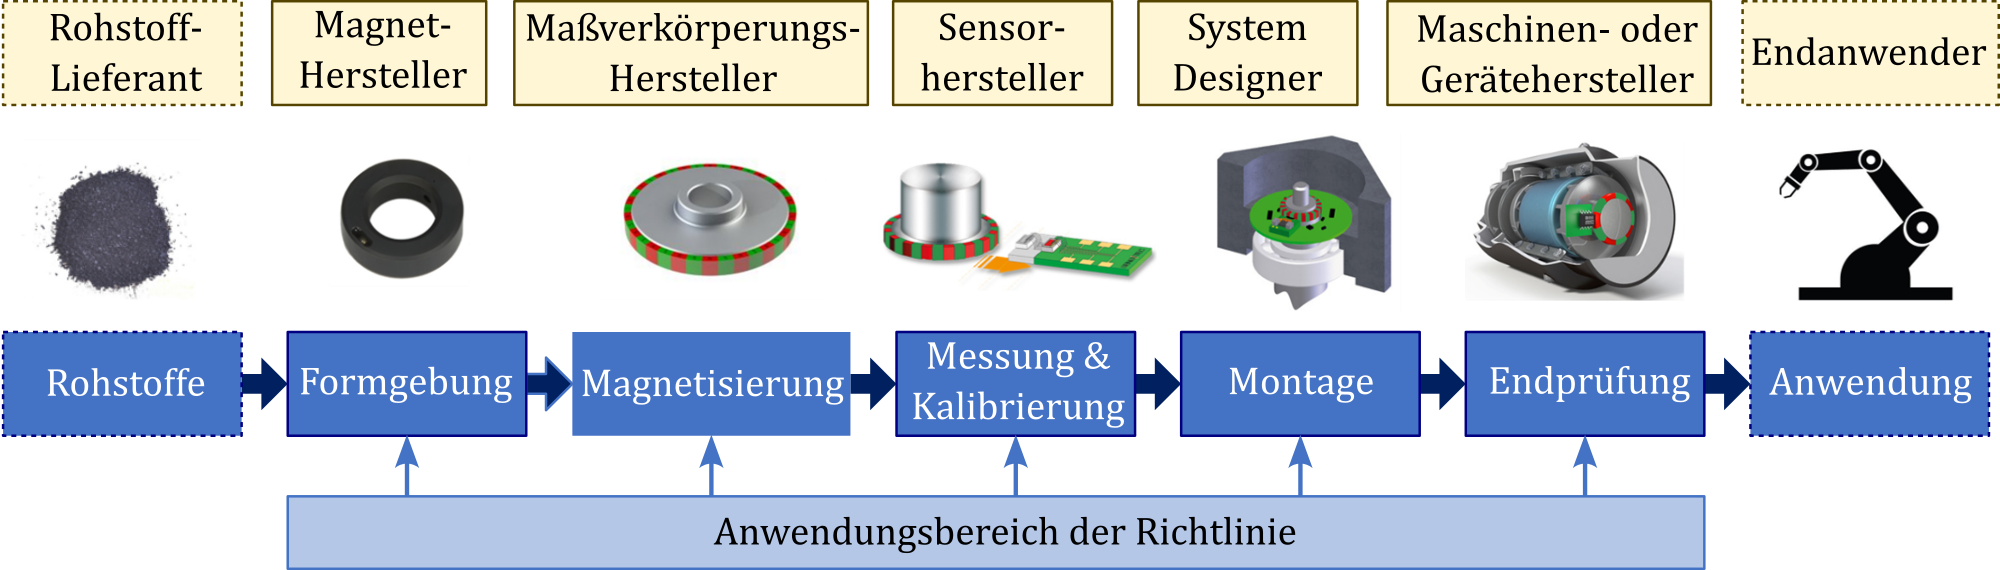
\includegraphics[width=1\linewidth,height=\textheight,keepaspectratio]{figures/sec01/01-value_chain.png}

}

\caption{\label{fig-sec01-value_chain}Wertschöpfungskette „Vom Rohstoff
bis zur Anwendung``}

\end{figure}%

Da die einzelnen Prozessschritte häufig von unterschiedlichen Akteuren
durchgeführt werden, entstehen an den Übergängen Schnittstellen
hinsichtlich der mechanischen und magnetischen Eigenschaften der
Maßverkörperung sowie ihrer Prüfung. Für diese Schnittstellen fehlen
bislang eine einheitliche \textbf{Terminologie} zur Beschreibung
magnetischer Maßverkörperungen, standardisierte
\textbf{Darstellungsregeln} sowie abgestimmte Verfahren zu ihrer
\textbf{Vermessung} und \textbf{Bewertung}. Eine zuverlässige
Qualitätsbewertung setzt insbesondere voraus, dass die verwendeten
Prüfverfahren eindeutig beschrieben und vergleichbar angewendet werden
können.

Unvollständige Informationen und uneinheitliche Bezeichnungen können an
den Schnittstellen zu \textbf{Missverständnissen und Fehlern} führen und
dadurch zusätzlichen Entwicklungsaufwand und Kosten verursachen. Werden
Anforderungen an magnetische Maßverkörperungen nicht eindeutig
beschrieben, erschwert dies zudem den Vergleich von Komponenten
unterschiedlicher Hersteller sowie die Auswahl geeigneter
Alternativprodukte oder Ersatzteile (Second Source).

\textbf{Ziel dieser Richtlinie} ist es, eine einheitliche Terminologie
sowie Regeln zur Beschreibung, Darstellung, Vermessung und Bewertung
magnetischer Maßverkörperungen zu schaffen. Es handelt sich um eine
Weiterentwicklung der DIN SPEC 91411 (Innomag 2022) und richtet sich an
Komponentenlieferanten, Hersteller und Anwender magnetischer Weg- und
Winkelmesssysteme.

\begin{tcolorbox}[enhanced jigsaw, arc=.35mm, bottomrule=.15mm, bottomtitle=1mm, breakable, colback=white, colbacktitle=quarto-callout-tip-color!10!white, colframe=quarto-callout-tip-color-frame, coltitle=black, left=2mm, leftrule=.75mm, opacityback=0, opacitybacktitle=0.6, rightrule=.15mm, title=\textcolor{quarto-callout-tip-color}{\faLightbulb}\hspace{0.5em}{Hinweis}, titlerule=0mm, toprule=.15mm, toptitle=1mm]

\emph{Diese Richtlinie ist als \textbf{lebendes Dokument} angelegt. In
der vorliegenden Fassung 1.x liegt der Schwerpunkt auf Terminologie,
Beschreibung, Darstellung, Einteilung und Grundlagen der Vermessung
magnetischer Maßverkörperungen. Weiterführende Inhalte, insbesondere zu
Prüfaufbau und Bewertung, werden in späteren Fassungen ergänzt.}

\end{tcolorbox}

\section{Geltungsbereich}\label{geltungsbereich}

Diese Richtlinie behandelt magnetische Maßverkörperungen als Komponenten
magnetischer Weg- und Winkelmesssysteme. Im Mittelpunkt stehen ihre
magnetische und geometrische Beschreibung, die Darstellung und
Spezifikation ihrer Eigenschaften sowie deren Vermessung und Bewertung.

Die eingeführte Terminologie und Beschreibungssystematik ist speziell
für magnetische Weg- und Winkelmesssysteme ausgelegt. Sie kann jedoch in
weiten Teilen auch auf mehrdimensionale magnetische Positionsmesssysteme
sowie allgemein auf die technische Beschreibung und Darstellung von
Dauermagneten übertragen werden.

Das Messsystem, der magnetische Sensor und der Herstellungsprozess der
Maßverkörperung werden nur insoweit betrachtet, wie dies für die
Beschreibung, Vermessung oder Bewertung der Maßverkörperung erforderlich
ist. Die Bewertung des vollständigen Messsystems bzw. der Endanwendung,
insbesondere seiner Positionsgenauigkeit, ist nicht Gegenstand dieser
Richtlinie.

Die Maßverkörperung wird damit grundsätzlich unabhängig von einem
bestimmten Herstellungsverfahren, Sensortyp oder einer konkreten
Anwendung beschrieben. Anforderungen an ihre Eigenschaften können sich
jedoch aus Herstellung, Sensorik und Anwendung ergeben.

\bookmarksetup{startatroot}

\chapter{Beispiele magnetischer Messsysteme}\label{sec-sec02}

Dieses Kapitel zeigt industrielle Beispiele magnetischer Weg- und
Winkelmesssysteme. Die Beispiele verdeutlichen, wie magnetische
Maßverkörperungen zusammen mit magnetischen Sensoren zur
Positionserfassung in realen Anwendungen eingesetzt werden. Sie dienen
als anschauliche Motivation für die in diesem Dokument eingeführten
Begriffe, Beschreibungsformen und Modellvorstellungen.

\section{Wegmesssystem in einer
Hinterachslenkung}\label{sec-sec02-hinterachslenkung}

Die Hinterachslenkung in einem Automobil bezeichnet das zusätzliche
Mitlenken der Hinterräder durch gezieltes Verstellen ihres Spurwinkels.
Moderne Systeme erreichen dabei je nach Ausführung Spurwinkel von bis zu
10°. Dadurch kann bei niedrigen Geschwindigkeiten der Wendekreis des
Fahrzeugs verkleinert und bei höheren Geschwindigkeiten die
Fahrstabilität erhöht werden. Eingesetzt wird diese Technologie
insbesondere in größeren Pkw, etwa in Limousinen, SUVs, Sportwagen und
Elektrofahrzeugen (Hägele 2014).

Für die Regelung der Hinterachslenkung ist eine robuste und
berührungslose Wegerfassung der Aktuatorposition erforderlich. Ein
magnetisches Messsystem kann hierfür die Verstellung auch unter
fahrzeugtypischen Umgebungsbedingungen wie Vibration,
Temperaturänderung, Verschmutzung und begrenztem Bauraum zuverlässig
erfassen.

\begin{figure}[h]

\centering{

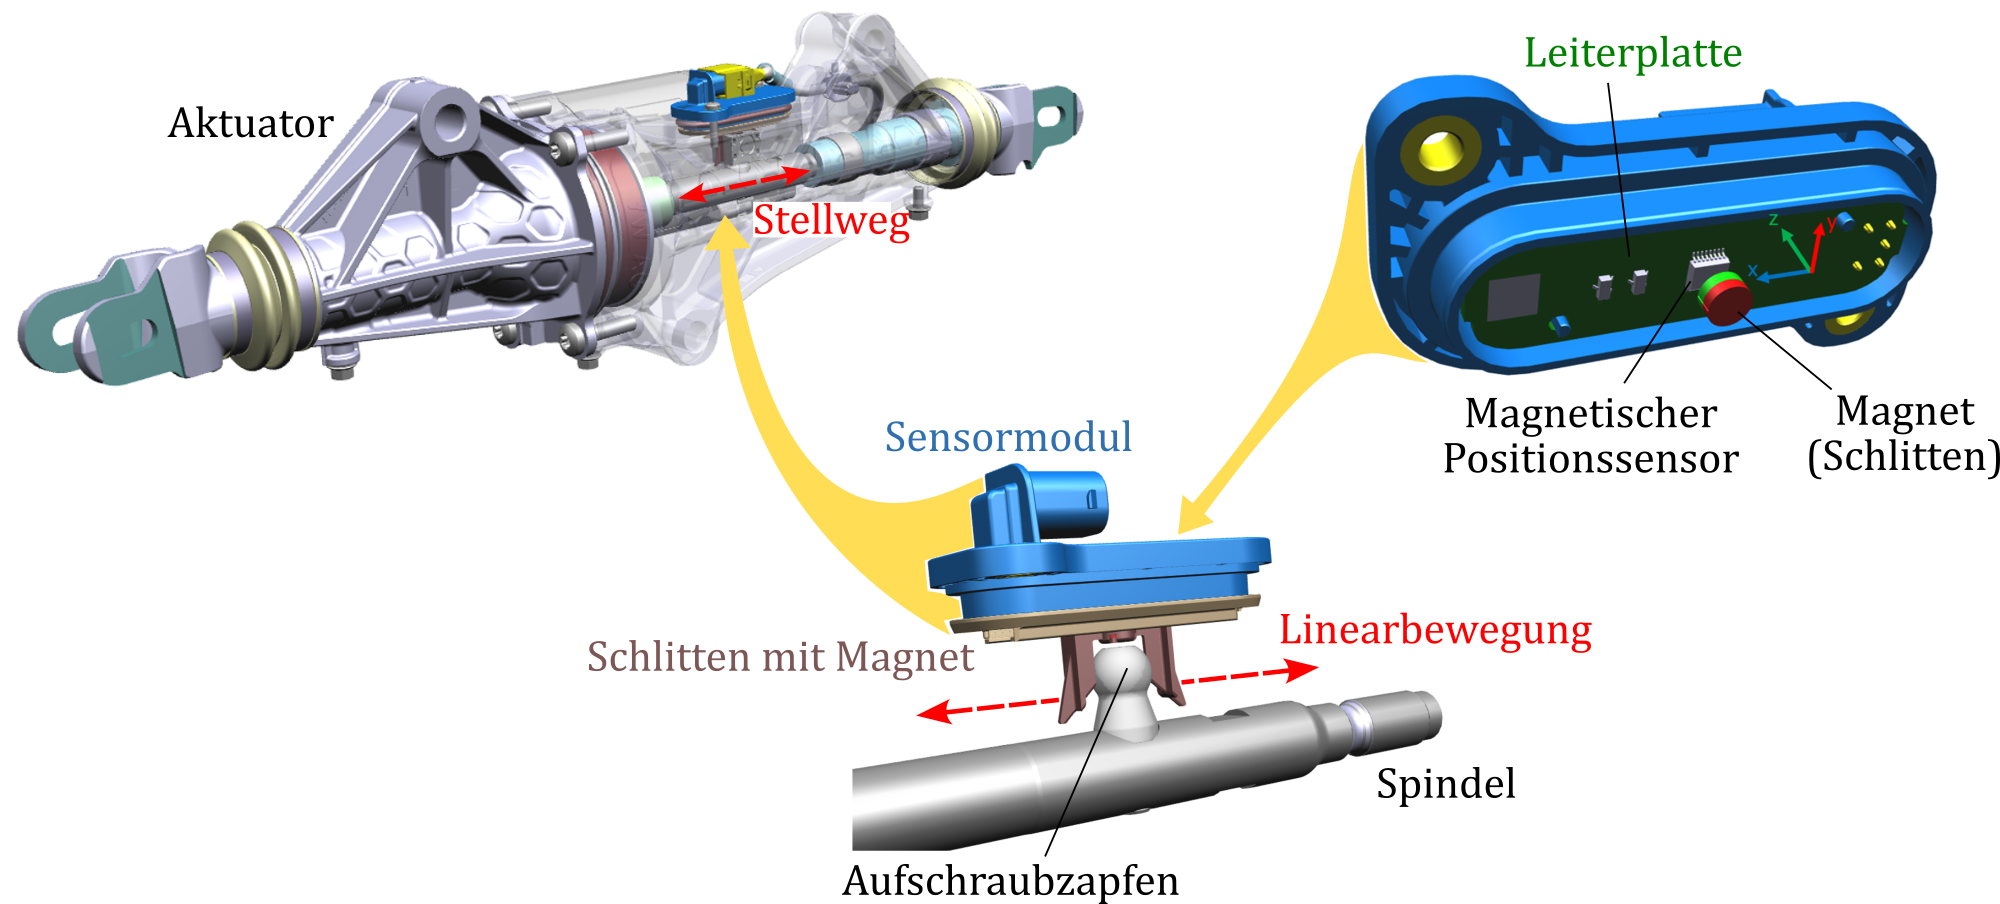
\includegraphics[width=1\linewidth,height=\textheight,keepaspectratio]{figures/sec02/01-linearweg_hinterachsenlenkung.png}

}

\caption[\label{fig-sec02-01-linearweg_hinterachsenlenkung}Beispiel
Wegmessung bei einer Hinterachslenkung]{\label{fig-sec02-01-linearweg_hinterachsenlenkung}Beispiel
Wegmessung bei einer Hinterachslenkung\footnotemark{}}

\end{figure}%
\footnotetext{Quelle: ZF
  Friedrichshafen AG (ZF Friedrichshafen AG 2026); redaktionelle
  Bearbeitung durch die Autoren.}

Abbildung~\ref{fig-sec02-01-linearweg_hinterachsenlenkung} zeigt ein
magnetisches Wegmesssystem, das zur Erfassung des Spurwinkels der
Hinterachse eingesetzt wird (ZF Friedrichshafen AG 2026). Der Spurwinkel
wird dabei mechanisch auf einen linearen Stellweg übersetzt. Je nach
Ausführung werden Stellwege bis 40 mm durch einen elektromechanischen
Aktuator eingestellt.

Zur Positionserfassung, insbesondere zur Erfassung der Neutralstellung,
ist an der Spindel ein Aufschraubzapfen montiert. Auf diesem befindet
sich ein Schlitten mit einem axial magnetisierten
NdFeB-Zylindermagneten, der als einfacher Dipolmagnet die magnetische
Maßverkörperung bildet. Der Magnet weist einen Durchmesser von 6 mm und
eine Höhe von 3 mm auf. Das blaue Sensormodul mit dem auf der
Leiterplatte montierten magnetischen Sensor ist oberhalb des Magneten
fest positioniert. Der Abstand zwischen Magnet und Sensor beträgt etwa 3
mm. Bei einer Veränderung des Spurwinkels bewegt sich der Magnet entlang
des linearen Stellwegs relativ zum fest montierten Sensor.

\begin{figure}[h]

\centering{

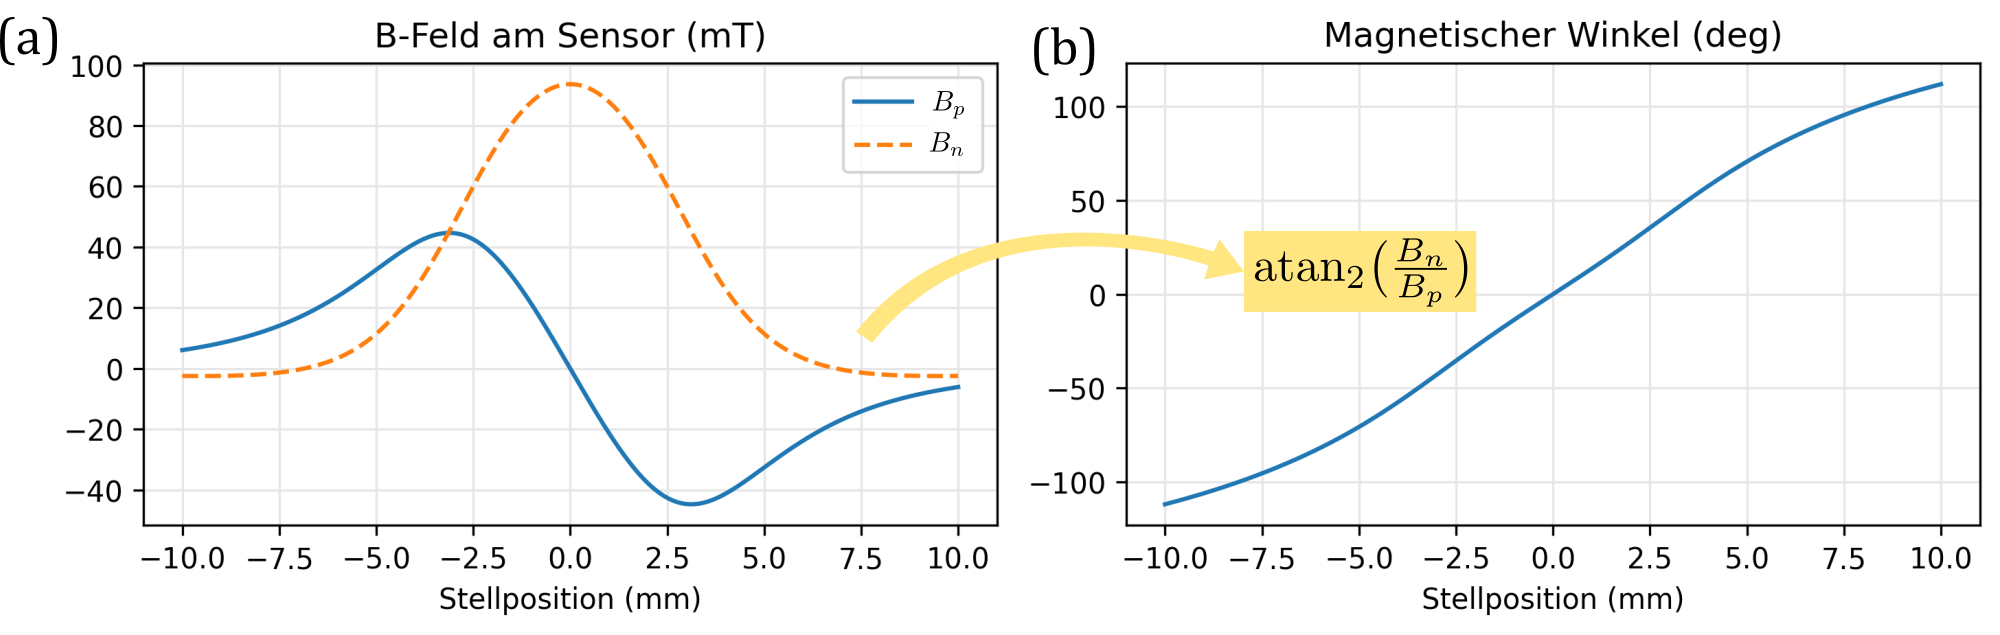
\includegraphics[width=1\linewidth,height=\textheight,keepaspectratio]{figures/sec02/02-linearweg_hinterachsenlenkung2.png}

}

\caption{\label{fig-sec02-02-linearweg_hinterachsenlenkung2}Positionsermittlung
bei linearen Wegmesssystemen}

\end{figure}%

Abbildung~\ref{fig-sec02-02-linearweg_hinterachsenlenkung2} (a) zeigt
die positionsabhängige Änderung der vom Sensor erfassten
Streufeldkomponenten für einen linearen Stellweg von 20 mm in diesem
System. Aus den beiden Feldkomponenten wird mit einem üblichen
Berechnungsschema ein magnetischer Winkel ermittelt (b). Im betrachteten
Stellbereich ist dieser streng monoton und ermöglicht dadurch eine
eindeutige Zuordnung der linearen Stellposition zum magnetischen Winkel.

Das Beispiel steht für einfach aufgebaute magnetische Wegmesssysteme,
die aufgrund ihrer Robustheit und Kosteneffizienz weit verbreitet sind.
Trotz des einfachen Grundprinzips kann die konkrete Einbausituation
komplex sein und erfordert eine sorgfältige Systemauslegung sowie eine
präzise und robuste Erfassung des Streufeldes.

\section{Winkelmesssystem in einem Elektromotor}\label{sec-sec02-emotor}

Die Bestimmung von Drehwinkel und Drehzahl ist eine zentrale
Voraussetzung für den geregelten Betrieb elektrischer Motoren.
Insbesondere bei geschlossenen Regelkreisen werden diese Größen
benötigt, um die Rotorlage zu bestimmen, die Ansteuerung der
Phasenströme darauf abzustimmen und Drehmoment sowie Drehzahl präzise zu
regeln. Hierfür können unterschiedliche Arten von Drehgebern eingesetzt
werden.

\begin{figure}[h]

\centering{

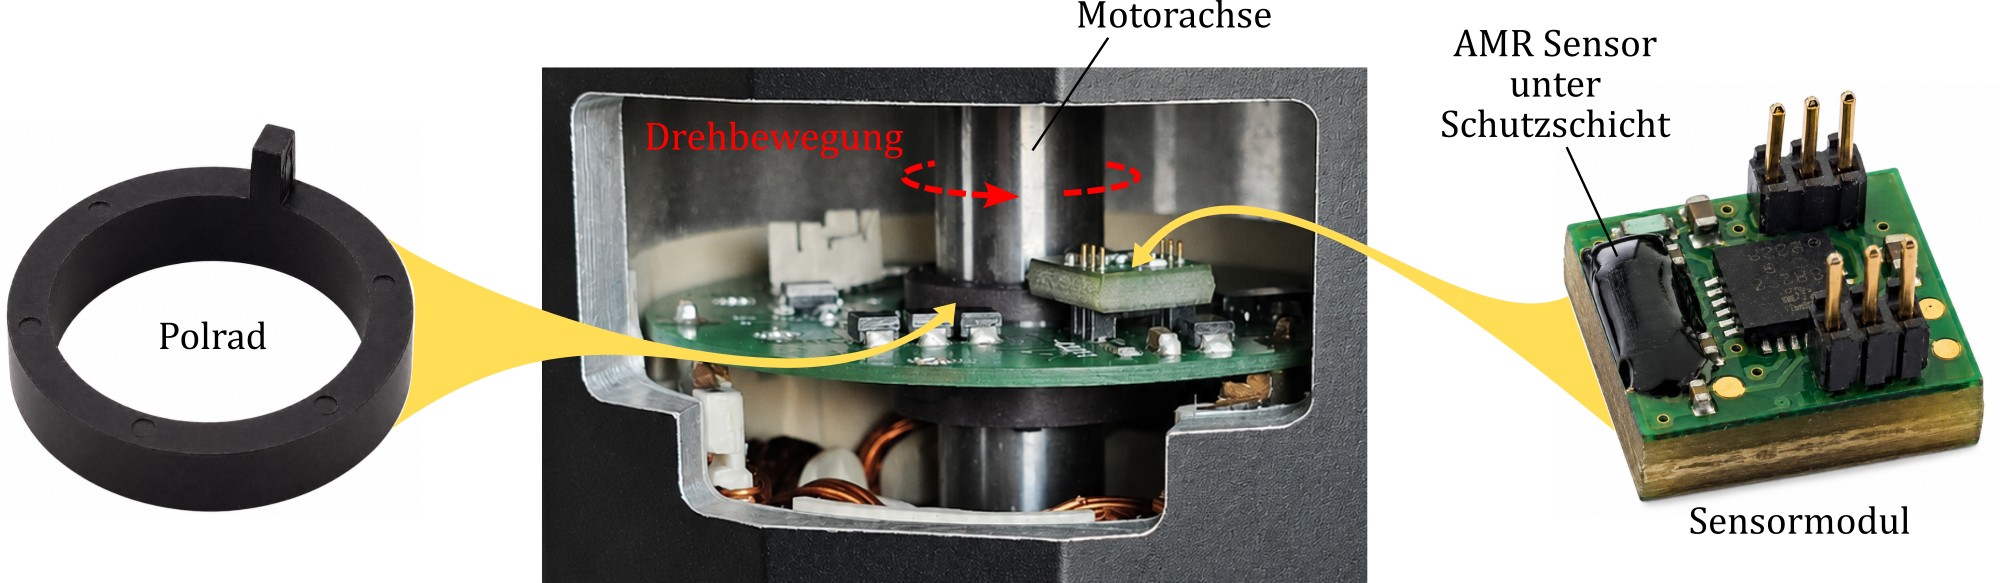
\includegraphics[width=1\linewidth,height=\textheight,keepaspectratio]{figures/sec02/03-emotor_drehgeber.png}

}

\caption[\label{fig-sec02-03-emotor_drehgeber}Beispiel Winkelmessung in
einem Elektromotor]{\label{fig-sec02-03-emotor_drehgeber}Beispiel Winkelmessung in
einem Elektromotor\footnotemark{}}

\end{figure}%
\footnotetext{Quelle der Abbildung: Sensitec GmbH;
  redaktionelle Aufbereitung durch die Autoren.}

Abbildung~\ref{fig-sec02-03-emotor_drehgeber} zeigt eine typische
Einbausituation eines magnetischen Drehgebers. Das Messsystem besteht
aus einem als Polrad ausgeführten magnetischen Maßstab aus
kunststoffgebundenem Hartferrit und einem darauf abgestimmten
Sensormodul. Der Maßstab weist zwei magnetische Spuren auf: eine
Inkrementalspur mit \(N_P=32\) Polen sowie eine Referenzspur mit einem
einzelnen Referenzpol. Eine Besonderheit des Maßstabs besteht darin,
dass die Referenzspur durch eine kleine, am Spritzgussteil ausgeformte
Erhebung („Nase``) realisiert wird, deren Bogenlänge der Pollänge der
Referenzspur entspricht.

Das Sensormodul besitzt auf seiner Oberseite einen GMR-Sensor zur
Erfassung der Referenzspur und auf seiner Unterseite einen AMR-Sensor
zur Erfassung der Inkrementalspur. Es gibt nach interner
Signalaufbereitung und Interpolation ein quadraturcodiertes A/B-Signal
mit 4096 Flanken pro Umdrehung sowie einen Referenzpuls Z pro Umdrehung
aus, siehe Abbildung~\ref{fig-sec02-04-emotor_drehgeber2} (a). Eine
typische Fehlerkurve des vollständigen Messsystems ist in Teilbild (b)
gezeigt.

\begin{figure}[h]

\centering{

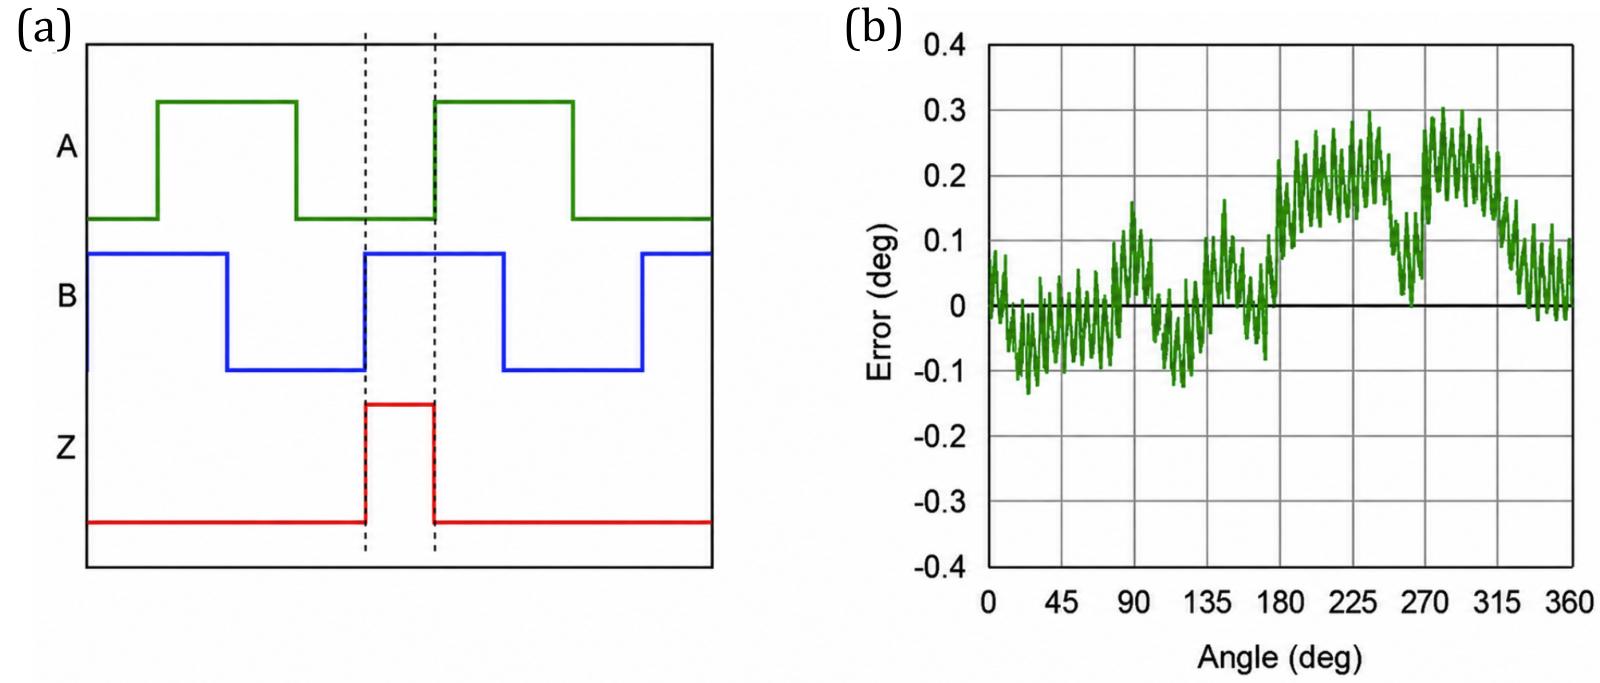
\includegraphics[width=1\linewidth,height=\textheight,keepaspectratio]{figures/sec02/04-emotor_drehgeber2.png}

}

\caption[\label{fig-sec02-04-emotor_drehgeber2}Ausgangssignale und
Winkelfehler des magnetischen Drehgebers]{\label{fig-sec02-04-emotor_drehgeber2}Ausgangssignale und
Winkelfehler des magnetischen Drehgebers\footnotemark{}}

\end{figure}%
\footnotetext{Quelle der Abbildung:
  Sensitec GmbH; redaktionelle Aufbereitung durch die Autoren.}

Das Beispiel veranschaulicht die reale Einbausituation und das
Zusammenwirken mehrerer magnetischer Spuren mit unterschiedlichen
Funktionen für die Realisierung eines magnetischen Winkelmesssystems.

\bookmarksetup{startatroot}

\chapter{Grundlagen des Messsystems}\label{sec-03}

In diesem Kapitel werden wichtige Grundlagen magnetischer Weg- und
Winkelmesssysteme beschrieben. Insbesondere werden Komponenten wie
Sensor und magnetische Maßverkörperung eingeführt und ihre Anordnung im
Messsystem beschrieben.

\section{Magnet und Magnetfeld}\label{sec-03-magnet_und_magnetfeld}

Die \textbf{Magnetisierung} \(\vec{M}\) (Einheit A/m) beschreibt den
magnetischen Zustand eines Materials infolge der Ausrichtung seiner
mikroskopischen magnetischen Dipolmomente und entspricht dem
magnetischen Moment pro Volumeneinheit. Die \textbf{magnetische
Polarisation} \(\vec{J}\) (Einheit T) ist eine dazu proportionale Größe,
\(\vec{J}=μ_0 \vec{M}\). Ein Körper mit permanenter Magnetisierung wird
als \textbf{Dauermagnet} bezeichnet (Jackson 1998; Petrascheck und
Schwabl 2023).

\begin{tcolorbox}[enhanced jigsaw, arc=.35mm, bottomrule=.15mm, bottomtitle=1mm, breakable, colback=white, colbacktitle=quarto-callout-tip-color!10!white, colframe=quarto-callout-tip-color-frame, coltitle=black, left=2mm, leftrule=.75mm, opacityback=0, opacitybacktitle=0.6, rightrule=.15mm, title=\textcolor{quarto-callout-tip-color}{\faLightbulb}\hspace{0.5em}{Hinweis}, titlerule=0mm, toprule=.15mm, toptitle=1mm]

\emph{Für den in diesem Dokument bevorzugt verwendeten Begriff
\textbf{Polarisation} wird in der Fachliteratur und Praxis meist der
proportionale Begriff \textbf{Magnetisierung} verwendet. Der Begriff
Polarisation wird in dieser Richtlinie bevorzugt, weil er eine
eindeutige Abgrenzung gegenüber dem Prozess der Magnetisierung
sicherstellt. Darüber hinaus entspricht diese Wahl der in der Praxis
verbreiteten Angabe der magnetischen Stärke von Dauermagneten in Tesla.}

\end{tcolorbox}

Das \textbf{Magnetfeld} ist ein physikalisches Feld, das von bewegten
elektrischen Ladungen oder magnetisierten Körpern erzeugt wird. Es
beschreibt den Zustand des Raums, in dem magnetische Kräfte wirken, und
wird durch die magnetische Feldstärke \(\vec{H}\) und die magnetische
Flussdichte \(\vec{B}\) charakterisiert. Um den häufig auftretenden
terminologischen Verwirrungen vorzubeugen, werden diese fundamentalen
physikalischen Größen in diesem Dokument vereinfachend als
\textbf{B-Feld} und \textbf{H-Feld} bezeichnet.

Die Felder \(\vec{B}\) und \(\vec{H}\) unterscheiden sich durch ihre
Einheiten und durch die Berücksichtigung der Magnetisierung. Sie stehen
in folgender Beziehung: \(\vec{B}=μ_0 (\vec{H}+\vec{M})\). Da im Kontext
dieser Richtlinie das Magnetfeld ausschließlich außerhalb einer
magnetischen Maßverkörperung betrachtet wird, also in einem Bereich, in
dem \(\vec{M}=0\) gilt, sind B- und H-Feld proportional und werden daher
synonym behandelt. Das Magnetfeld im Außenraum eines Dauermagneten wird
auch oft als \textbf{Streufeld} bezeichnet.

Die Größen \(\vec{M}, \vec{J}, \vec{H}\) und \(\vec{B}\) entsprechen den
gleichnamigen fundamentalen Feldgrößen aus den Maxwellschen Gleichungen
in der Materie (Jackson 1998; Petrascheck und Schwabl 2023).

Das Magnetfeld eines Körpers ergibt sich aus der Überlagerung der
Magnetfelder seiner mikroskopischen Dipolmomente, die seine Polarisation
ausmachen. Bei homogener Polarisation weist insbesondere das Streufeld
des Körpers eine hohe Ähnlichkeit mit dem Feld eines elementaren Dipols
auf und wird im allgemeinen Sprachgebrauch dann häufig vereinfachend als
\textbf{Dipolfeld} bezeichnet.

\begin{figure}[h]

\centering{

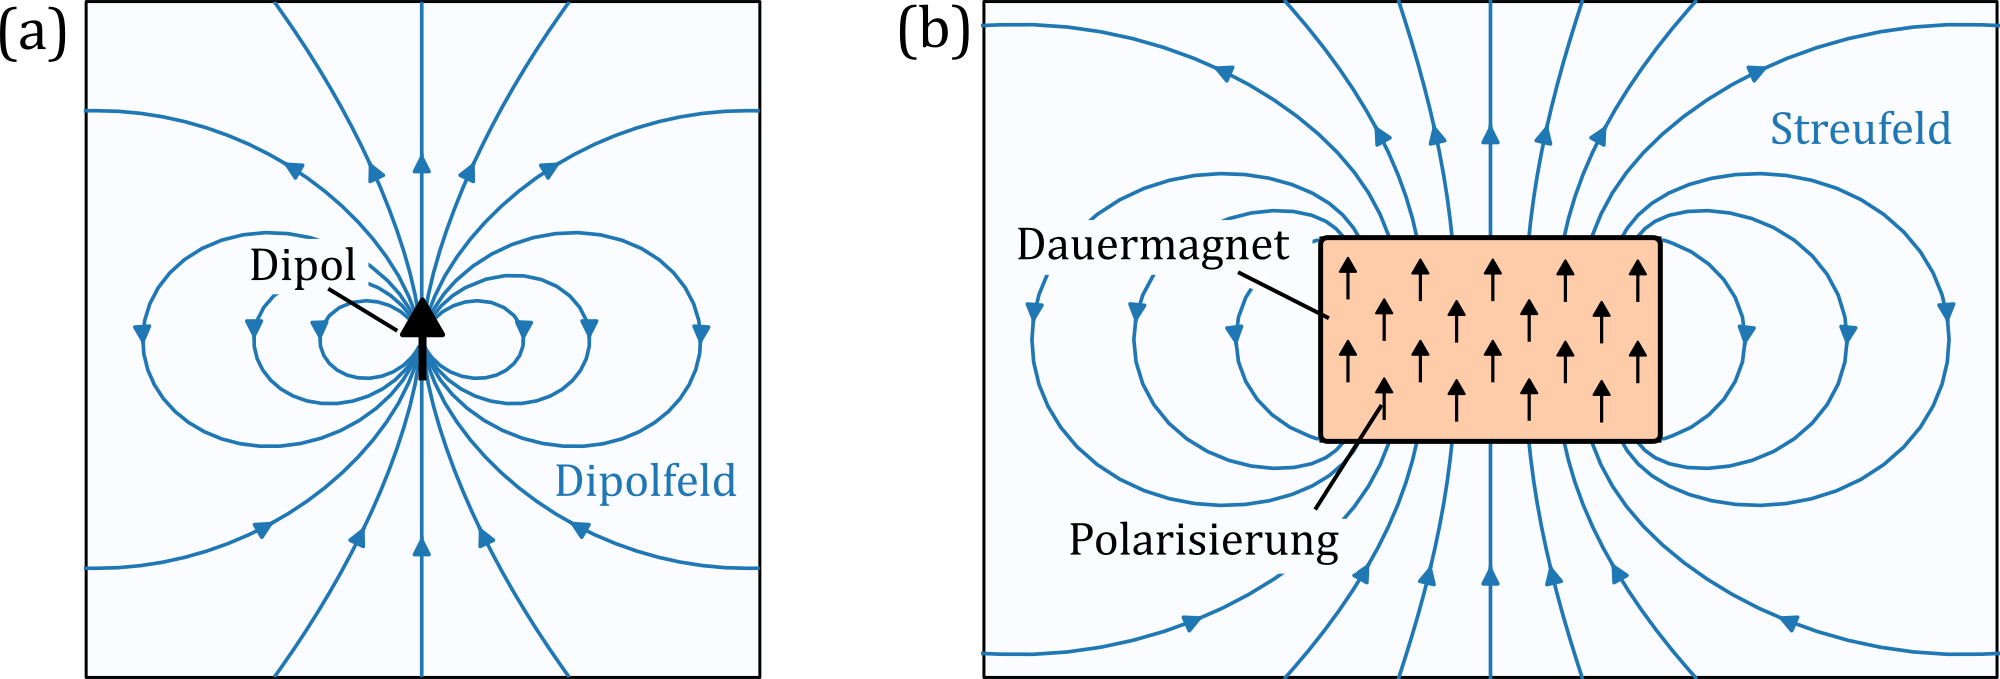
\includegraphics[width=0.9\linewidth,height=\textheight,keepaspectratio]{figures/sec03/01-magnet_und_magnetfeld.png}

}

\caption{\label{fig-sec03-01-magnet_und_magnetfeld}Physikalische
Grundbegriffe}

\end{figure}%

Abbildung~\ref{fig-sec03-01-magnet_und_magnetfeld} (a) zeigt das Feld
eines Punktdipols. Teilbild (b) zeigt das Streufeld und die Polarisation
eines würfelförmigen Dauermagneten im Querschnitt; die homogene
magnetische Polarisation ist durch schwarze Pfeile dargestellt. Die
dargestellten Feldlinien basieren auf einer numerischen Simulation. Es
wird deutlich, dass das Streufeld eines endlichen Magneten in großem
Abstand eine hohe Ähnlichkeit mit dem Dipolfeld aufweist, im Nahbereich
jedoch deutliche Abweichungen zeigt.

Dauermagnete können komplexe Polarisation aufweisen.
\textbf{Dipolmagnete} sind Dauermagnete, deren Magnetfeld im
betrachteten Bereich vom Dipolanteil dominiert wird, siehe auch
Abbildung~\ref{fig-sec03-01-magnet_und_magnetfeld} (b). Typischerweise
handelt es sich dabei um Körper mit quasi-homogener Polarisation.
\textbf{Multipolmagnete} weisen mehrere Polarisationsbereiche auf. Sie
können beispielsweise aus mehreren Dipolmagneten zusammengesetzt sein.
\textbf{Magnetische Maßstäbe} sind hingegen Dauermagnete mit einem
typischerweise entlang der Oberfläche verlaufenden streifenförmigen
Polarisationsmuster. Diese Einteilung dient vorwiegend der groben
Unterscheidung des Komplexitätsgrades eines Dauermagneten und wird in
Kapitel~\ref{sec-07} näher ausgeführt.

\section{Anordnung des
Messsystems}\label{sec-03-anordnung_des_messsystems}

\textbf{Magnetische Weg- und Winkelmesssysteme} bestimmen die
Relativposition zweier mechanischer Bauteile entlang einer festgelegten
Bewegungskoordinate. Sie bestehen im Wesentlichen aus einem
Dauermagneten und einem magnetischen Sensor, die jeweils einem der
relativ zueinander bewegten Bauteile zugeordnet sind. Der Dauermagnet
stellt die für die Positionsbestimmung erforderliche Ortsinformation
durch die räumliche Struktur seines Streufeldes bereit und wird in
diesem Zusammenhang als \textbf{magnetische Maßverkörperung} bezeichnet.
Der Sensor erfasst das von der Maßverkörperung erzeugte Magnetfeld.

Ausgehend von der Messaufgabe und den damit verbundenen geometrischen
Randbedingungen wird eine geeignete \textbf{geometrische Anordnung} von
Sensor und Maßverkörperung gewählt. Dabei lassen sich magnetische Weg-
und Winkelmesssysteme trotz zahlreicher konstruktiver
Realisierungsmöglichkeiten zweckmäßig in vier Gruppen einteilen:

\begin{enumerate}
\def\labelenumi{\arabic{enumi}.}
\tightlist
\item
  \textbf{Lineare Anordnung}: Sensor und Maßverkörperung bewegen sich
  entlang einer geradlinigen Bahn bei unveränderter relativer
  Orientierung zueinander. Die Bewegung erfolgt meist parallel zu einer
  Oberfläche der Maßverkörperung. Ein Beispiel hierfür ist die Anwendung
  nach Kapitel~\ref{sec-sec02-hinterachslenkung}.
\item
  \textbf{Radiale Anordnung}: Eine rotationssymmetrische Maßverkörperung
  rotiert um ihre Rotationsachse. Der Sensor ist seitlich zur
  Rotationsachse an einer Mantelfläche der Maßverkörperung angeordnet.
  Ein Beispiel hierfür ist die Anwendung nach
  Kapitel~\ref{sec-sec02-emotor}.
\item
  \textbf{Axiale Anordnung}: Eine rotationssymmetrische Maßverkörperung
  rotiert um ihre Rotationsachse. Der Sensor ist stirnseitig zur
  Rotationsachse an einer Stirnfläche der Maßverkörperung angeordnet.
\item
  \textbf{Allgemeine Anordnung}: Geometrische Anordnungen, die keiner
  der drei zuvor genannten Gruppen zweckmäßig zugeordnet werden.
\end{enumerate}

\begin{figure}[h]

\centering{

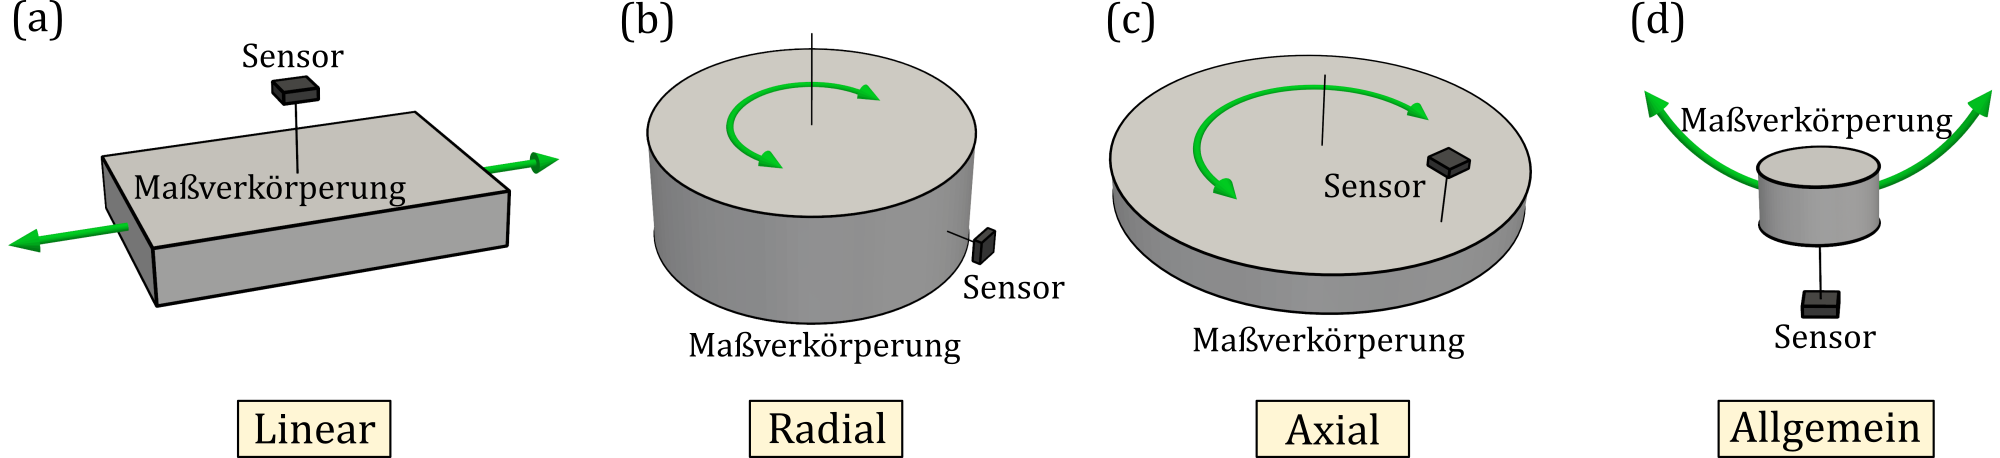
\includegraphics[width=1\linewidth,height=\textheight,keepaspectratio]{figures/sec03/02-geometrische_anordnung.png}

}

\caption{\label{fig-sec03-02-geometrische_anordnung}Geometrische
Anordnungen eines Messsystems}

\end{figure}%

Abbildung~\ref{fig-sec03-02-geometrische_anordnung} veranschaulicht die
vier geometrischen Anordnungstypen: (a) eine lineare, (b) eine radiale,
(c) eine axiale und (d) eine allgemeine Anordnung. Die allgemeine
Anordnung ist hier anhand einer typischen eindimensionalen
„Joystick-Realisierung`` dargestellt, bei der sich während der Bewegung
sowohl die relative Orientierung als auch der Abstand zwischen
Maßverkörperung und Sensor verändern.

\begin{tcolorbox}[enhanced jigsaw, arc=.35mm, bottomrule=.15mm, bottomtitle=1mm, breakable, colback=white, colbacktitle=quarto-callout-tip-color!10!white, colframe=quarto-callout-tip-color-frame, coltitle=black, left=2mm, leftrule=.75mm, opacityback=0, opacitybacktitle=0.6, rightrule=.15mm, title=\textcolor{quarto-callout-tip-color}{\faLightbulb}\hspace{0.5em}{Hinweis}, titlerule=0mm, toprule=.15mm, toptitle=1mm]

\emph{Der \textbf{Fokus der Richtlinie} liegt auf linearen, radialen und
axialen Anordnungen, die einen großen Teil magnetischer Weg- und
Winkelmesssysteme abdecken. Die in dieser Richtlinie eingeführte
Terminologie ist in weiten Teilen auf allgemeine Anordnungen
übertragbar. Die nachfolgend eingeführte Koordinatenwahl ist jedoch
insbesondere für lineare, radiale und axiale Anordnungen zweckmäßig.}

\end{tcolorbox}

\section{Koordinatensystem der
Maßverkörperung}\label{sec-03-koordinatensystem_der_mauxdfverkuxf6rperung}

Aus der geometrischen Anordnung ergibt sich eine \textbf{zweckmäßige
Koordinatenwahl} zur Beschreibung des Messsystems.

Für die Beschreibung des Messsystems wird eine Bewegungsrichtung des
Sensors oder der Maßverkörperung als \textbf{Vorwärtsbewegung}
festgelegt. Die \textbf{p-Richtung} mit dem Richtungsvektor
\(\vec{e}_p\) zeigt in Richtung der daraus resultierenden relativen
Bewegung des Sensors und wird als \textbf{Längsrichtung} bezeichnet.

Die \textbf{funktionale Oberfläche} der Maßverkörperung ist die dem
Sensor zugewandte, für die magnetische Abtastung maßgebende
Bezugsfläche. Bei linearen Anordnungen verläuft sie parallel zur
Relativbewegung von Sensor und Maßverkörperung; bei radialen und axialen
Anordnungen entspricht sie der dem Sensor zugewandten Mantel-
beziehungsweise Stirnfläche. Sie kann mit einer physischen Oberfläche
der Maßverkörperung zusammenfallen oder als gedachte Bezugsfläche
festgelegt werden. Die \textbf{n-Richtung} mit dem Richtungsvektor
\(\vec{e}_n\) steht senkrecht zur funktionalen Oberfläche und zeigt zum
Sensor.

Bei linearen, radialen und axialen Anordnungen stehen die
Richtungsvektoren \(\vec{e}_p\) und \(\vec{e}_n\) damit immer senkrecht
zueinander. Die \textbf{o-Richtung} mit dem Richtungsvektor
\(\vec{e}_o\) wird als dritte rechtshändige Koordinatenrichtung
festgelegt. Sie verläuft parallel zur funktionalen Oberfläche und wird
als \textbf{Querrichtung} bezeichnet.

Mit einem festgelegten \textbf{Ursprung} \(O_M\), der auf der
funktionalen Oberfläche liegt, bilden die Richtungen \(p\), \(o\) und
\(n\) ein rechtshändiges Koordinatensystem (KS), das als
\textbf{Maßverkörperungs-KS} bezeichnet wird. Es bildet den Bezug für
die Beschreibung von Geometrie und magnetischer Struktur der
Maßverkörperung, ihres Streufeldes sowie der Positionierung des Sensors.

Die funktionale Oberfläche der Maßverkörperung entspricht dann n=0; die
n-Koordinate gibt den Abstand von ihr an und wird als Messhöhe
bezeichnet. Die \textbf{Messhöhe} des Sensors ist in linearen, radialen
und axialen Anwendungen typischerweise konstant.

Bei linearen Anordnungen wird eine kartesische, bei radialen und axialen
Anordnungen eine zylindrische Koordinatendarstellung verwendet. In den
zylindrischen Fällen beschreibt die p-Koordinate die Winkelposition. Da
diese in der Praxis häufig als zugehörige Bogenlänge angegeben wird, ist
auf die \textbf{verwendeten Einheiten} entsprechend zu achten.

\begin{figure}[h]

\centering{

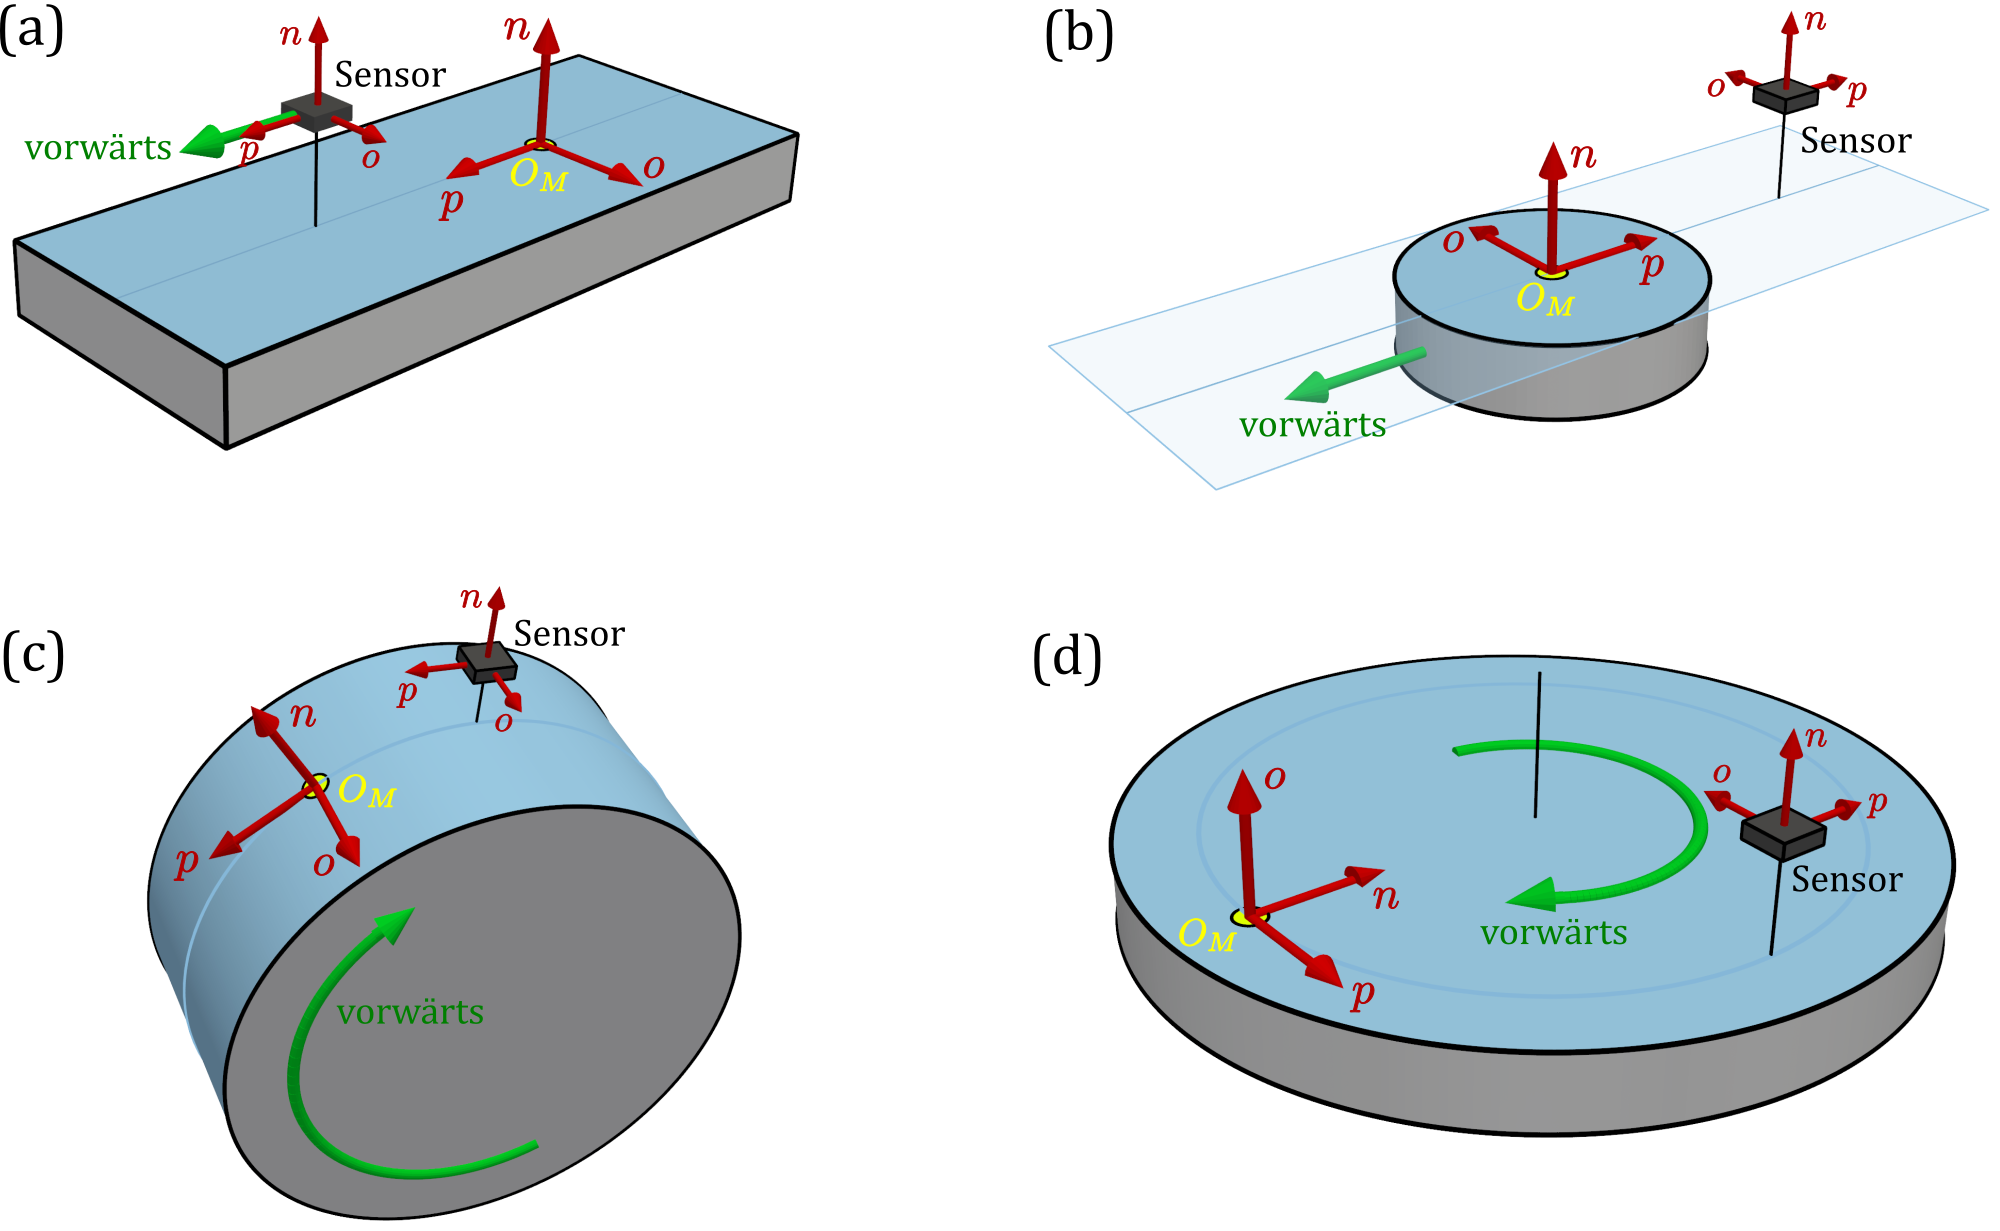
\includegraphics[width=0.9\linewidth,height=\textheight,keepaspectratio]{figures/sec03/03_koordinatenrichtungen.png}

}

\caption{\label{fig-sec03-03-koordinatenrichtungen}Wahl der
Koordinatenrichtungen}

\end{figure}%

Abbildung~\ref{fig-sec03-03-koordinatenrichtungen} zeigt verschiedene
Anordnungen von Sensor und Maßverkörperung sowie eine jeweils
zweckmäßige Wahl des Maßverkörperungs-KS. Die Teilbilder (a) und (b)
zeigen lineare Anordnungen, Teilbild (c) eine radiale und Teilbild (d)
eine axiale Anordnung.

Die funktionale Oberfläche der Maßverkörperung ist in der Abbildung blau
hervorgehoben. In Teilbild (b) ist sie als gedachte Fortsetzung über die
Seitenfläche der Maßverkörperung hinaus dargestellt. Die
Vorwärtsbewegung ist grün eingezeichnet. Sie bezieht sich in Teilbild
(a) auf die Bewegung des Sensors und in den übrigen Teilbildern auf die
Bewegung der Maßverkörperung.

Aus der funktionalen Oberfläche und der Vorwärtsbewegung werden die
Koordinatenrichtungen p, o und n wie beschrieben festgelegt. Das daraus
resultierende Maßverkörperungs-KS ist rot dargestellt; sein beispielhaft
gewählter Ursprung \(O_M\) ist gelb markiert. Zusätzlich sind die
Koordinatenrichtungen an der jeweiligen Sensorlage eingezeichnet.

\begin{tcolorbox}[enhanced jigsaw, arc=.35mm, bottomrule=.15mm, bottomtitle=1mm, breakable, colback=white, colbacktitle=quarto-callout-tip-color!10!white, colframe=quarto-callout-tip-color-frame, coltitle=black, left=2mm, leftrule=.75mm, opacityback=0, opacitybacktitle=0.6, rightrule=.15mm, title=\textcolor{quarto-callout-tip-color}{\faLightbulb}\hspace{0.5em}{Hinweis}, titlerule=0mm, toprule=.15mm, toptitle=1mm]

\emph{Im allgemeinen Sprachgebrauch wird häufig von \textbf{Achsen}
anstelle von Koordinatenrichtungen gesprochen. Davon wird hier
abgeraten, da bei radialen und axialen Anordnungen einzelne
Koordinatenrichtungen ortsabhängig sind und sich ihre Orientierung
ändern kann. Der Begriff Achse kann daher fälschlich eine feste
Raumrichtung suggerieren.}

\end{tcolorbox}

\section{Orientierung magnetischer
Größen}\label{sec-03-orientierung_magnetischer_gruxf6uxdfen}

Zur Beschreibung der Orientierung magnetischer Größen relativ zur
funktionalen Oberfläche werden häufig die Bezeichnungen \textbf{in-plane
(IP)} und \textbf{out-of-plane (OOP)} verwendet. Eine magnetische Größe
ist IP-orientiert, wenn sie parallel zur funktionalen Oberfläche liegt,
und OOP-orientiert, wenn sie senkrecht dazu steht. Das bedeutet, dass
sowohl die \(p\)- als auch die \(o\)-Richtung in-plane liegen, während
die n-Richtung out-of-plane orientiert ist. Entsprechend sind
beispielsweise die Polarisationskomponenten \(J_p\) und \(J_o\)
IP-Komponenten und \(J_n\) eine OOP-Komponente.

Bei den in dieser Richtlinie betrachteten linearen, radialen und axialen
Anordnungen werden für die Positionsmessung jedoch \textbf{überwiegend
magnetische Größen in \(p\)- und \(n\)-Richtung} genutzt. Die
\(o\)-Komponente der Polarisation beziehungsweise des Magnetfeldes
spielt für die betrachteten Messprinzipien in der Regel keine
unmittelbare Rolle. Die Bezeichnung IP wird daher in dieser Richtlinie
überwiegend für in \(p\)-Richtung orientierte Polarisationen
beziehungsweise für die \(p\)-Komponente des Magnetfeldes verwendet. Die
Bezeichnung OOP bezieht sich entsprechend auf die \(n\)-Richtung.

\section{Indexkonventionen}\label{sec-03-indexkonvention}

Viele der in diesem Dokument verwendeten Größen beziehen sich auf
bestimmte Elemente magnetischer Messsysteme oder auf charakteristische
Merkmale des Magnetfeldes. Zur Kennzeichnung dieses Bezugs werden die
Kürzel in Tabelle~\ref{tbl-bezugsindizes} als untere Bezugsindizes
verwendet.

\begingroup
\footnotesize
\renewcommand{\baselinestretch}{1.12}\selectfont
\setlength{\tabcolsep}{5pt}
\setlength{\extrarowheight}{2.5pt}
\renewcommand{\arraystretch}{1.15}
{\begin{longtable}[]{clcl}
\caption{Kürzel für Bezugsindizes}\label{tbl-bezugsindizes}\tabularnewline
\arrayrulecolor{tableouterrule}
\toprule\noalign{}
\rowcolor{zebrahead}
\textbf{Kürzel} & \textbf{Bezug} & \textbf{Kürzel} & \textbf{Bezug} \\
\arrayrulecolor{tableheadrule}
\specialrule{0.35pt}{0pt}{0pt}
\endhead
\arrayrulecolor{tableouterrule}
\specialrule{0.30pt}{0pt}{0pt}
\endlastfoot
\rowcolor{zebralight}
\textbf{M} & Maßverkörperung & \textbf{F} & Feld \\
\arrayrulecolor{tableline}
\specialrule{0.15pt}{0pt}{0pt}
\rowcolor{zebradark}
\textbf{S} & Sensor & \textbf{P} & Pol \\
\arrayrulecolor{tableline}
\specialrule{0.15pt}{0pt}{0pt}
\rowcolor{zebralight}
\textbf{T} & Struktur / Spur & \textbf{N} & Nullstelle \\
\arrayrulecolor{tableline}
\specialrule{0.15pt}{0pt}{0pt}
\rowcolor{zebradark}
\textbf{Z} & Zone & \textbf{A} & Peak (apex) \\
\arrayrulecolor{tableline}
\specialrule{0.15pt}{0pt}{0pt}
\rowcolor{zebralight}
& & \textbf{G} & Grenzwert \\
\arrayrulecolor{tableline}
\specialrule{0.15pt}{0pt}{0pt}
\end{longtable}
}
\endgroup

Darüber hinaus werden \textbf{Ordnungsindizes} verwendet, um einzelne
Objekte oder Merkmale zu nummerieren und eindeutig zu kennzeichnen. Sie
werden als obere Indizes in runden Klammern geführt.

Der Ordnungsindex \(i\) wird für Spuren und Spurfelder verwendet. Für
weitere Struktur- und Feldmerkmale wird der Ordnungsindex \(j\)
eingesetzt. Gleiche Ordnungsindizes stellen dabei nicht grundsätzlich
eine Zuordnung zwischen unterschiedlichen Objekttypen dar.
Beispielsweise muss Pol 3 nicht notwendigerweise Zone 3 zugeordnet sein.

Sind zur Beschreibung eines Objekts innerhalb einer Spur mehrere
Ordnungsindizes erforderlich, werden diese durch ein Komma getrennt. Der
erste Ordnungsindex gibt dabei die Spur an. Beispielsweise bezeichnet
\(l_P^{(2,5)}\) die Länge von Pol 5 der Spur 2.

Bei Größen, die sich auf zwei Spuren oder Spurfelder beziehen, wird der
jeweilige Bezugsindex doppelt geführt. So kennzeichnet „TT`` eine
Beziehung zwischen zwei Spuren und „FF`` eine Beziehung zwischen zwei
Spurfeldern. Beispielsweise bezeichnet \(w_{TT}^{(3,4)}\) den
Spurabstand zwischen Spur 3 und Spur 4. Bei gerichteten Größen wie dem
Versatz ist die Reihenfolge der Ordnungsindizes zu beachten.

\begin{tcolorbox}[enhanced jigsaw, arc=.35mm, bottomrule=.15mm, bottomtitle=1mm, breakable, colback=white, colbacktitle=quarto-callout-tip-color!10!white, colframe=quarto-callout-tip-color-frame, coltitle=black, left=2mm, leftrule=.75mm, opacityback=0, opacitybacktitle=0.6, rightrule=.15mm, title=\textcolor{quarto-callout-tip-color}{\faLightbulb}\hspace{0.5em}{Hinweis}, titlerule=0mm, toprule=.15mm, toptitle=1mm]

\emph{Zur Verbesserung der Lesbarkeit sollen Ordnungsindizes weggelassen
werden, sofern die Zuordnung aus dem Kontext eindeutig hervorgeht.
Besitzt ein magnetischer Maßstab beispielsweise nur eine Spur, soll
anstelle von \(w_T^{(1)}\) die verkürzte Schreibweise \(w_T\) verwendet
werden.}

\end{tcolorbox}

\bookmarksetup{startatroot}

\chapter{Magnetische Struktur der Maßverkörperung}\label{sec-04}

Kapitel~\ref{sec-03} führt die magnetische Maßverkörperung und ein ihr
zugeordnetes Koordinatensystem ein. Im Folgenden werden ihre
geometrische und magnetische Struktur beschrieben sowie
Darstellungsregeln und Begriffe für eine technisch detaillierte
Strukturbeschreibung festgelegt.

\section{Magnetisierte Zonen}\label{sec-04-magnetisierte_zonen}

Magnetische Maßverkörperungen weisen häufig \textbf{periodisch
strukturierte} oder aufeinander folgende Bereiche alternierend
ausgerichteter Polarisation auf. In solchen Fällen lassen sich klar
abgegrenzte Bereiche identifizieren, die voneinander getrennten, jedoch
meist identisch oder ähnlich aufgebauten Abschnitten entsprechen, die
gemeinsam das Gesamtsystem bilden.

Um diese strukturellen Einheiten präzise beschreiben und individuell
referenzieren zu können, wird der Begriff der \textbf{magnetisierten
Zone} eingeführt. Eine magnetisierte Zone ist ein zusammenhängendes,
geometrisch einfaches magnetisiertes Volumen, in dem die magnetische
Polarisation in ihrer räumlichen Verteilung bekannt ist und einen
endlichen Mittelwert aufweist. Zonen dienen der systematischen Zerlegung
der Polarisation einer Maßverkörperung in klar definierte Abschnitte,
die einzeln analysiert, nummeriert und im Zuge einer Vermessung oder
Modellbildung charakterisiert werden. Die Zerlegung einer
Polarisationsverteilung in Zonen entspricht mathematisch einer
Diskretisierung.

\begin{tcolorbox}[enhanced jigsaw, arc=.35mm, bottomrule=.15mm, bottomtitle=1mm, breakable, colback=white, colbacktitle=quarto-callout-tip-color!10!white, colframe=quarto-callout-tip-color-frame, coltitle=black, left=2mm, leftrule=.75mm, opacityback=0, opacitybacktitle=0.6, rightrule=.15mm, title=\textcolor{quarto-callout-tip-color}{\faLightbulb}\hspace{0.5em}{Hinweis}, titlerule=0mm, toprule=.15mm, toptitle=1mm]

\emph{Die \textbf{magnetisierte Zone} ist begrifflich klar von der
\textbf{magnetischen Domäne} (Weißsche Bezirke) abzugrenzen. Domänen
sind meist kleine Bereiche einheitlicher Polarisation, die infolge
mikromagnetischer Wechselwirkungen entstehen, während Zonen im Sinne
dieses Dokuments strukturelle Einheiten zur Beschreibung der
Polarisationsverteilung darstellen. Eine Übereinstimmung ist im
Einzelfall möglich, im Allgemeinen jedoch nicht gegeben.}

\end{tcolorbox}

Besonders anschaulich wird diese Einteilung, wenn eine Maßverkörperung
aus mehreren homogenen Dipolmagneten aufgebaut ist -- in diesem Fall
entspricht jeder einzelne Dipolmagnet einer eigenen Zone. Ebenso
entsteht bei magnetischen Maßstäben, deren Polarisationsmuster durch
schrittweises Einschreiben magnetisierter Bereiche erzeugt wird, bei
jedem Schreibvorgang eine Zone in der unmittelbaren Umgebung des
Schreibkopfes.

\begin{figure}[h]

\centering{

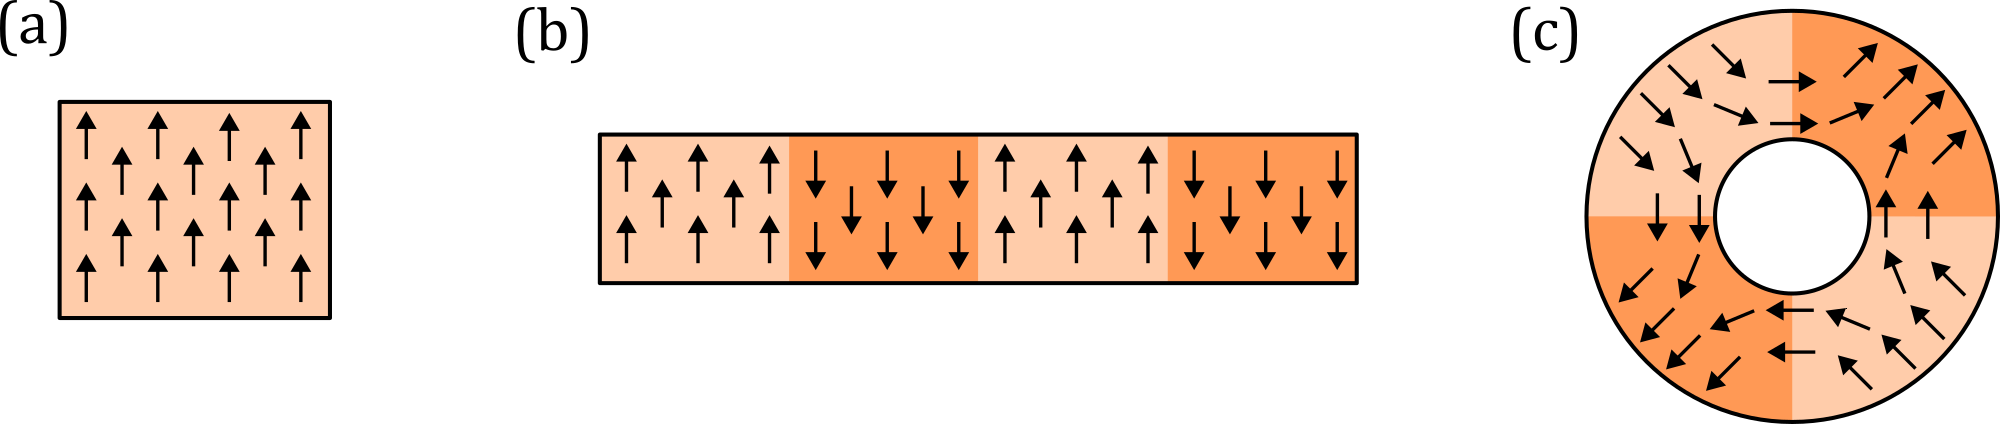
\includegraphics[width=0.9\linewidth,height=\textheight,keepaspectratio]{figures/sec04/01-zone_sketch1.png}

}

\caption{\label{fig-sec04-01-zone_sketch1}Magnetische Polarisation und
magnetisierte Zonen}

\end{figure}%

In Abbildung~\ref{fig-sec04-01-zone_sketch1} sind Beispiele für typische
magnetisierte Strukturen skizziert. Teilbild (a) zeigt einen homogen
magnetisierten Dipolmagneten, der eine einzige Zone bildet. Teilbild (b)
zeigt einen Multipolmagneten mit alternierender Polarisation entlang der
Längsachse. Die unterschiedlich polarisierten Bereiche sind durch
Schattierung hervorgehoben und veranschaulichen eine sinnvolle
Zoneneinteilung. (c) zeigt einen Quadrupolring mit stark inhomogener
Polarisation. Aufgrund seiner periodischen Struktur kann dennoch eine
sinnvolle Zoneneinteilung vorgenommen werden.

Die mittlere \textbf{Polarisation einer Zone} \(\vec{J}_Z\) ergibt sich
aus dem Integralmittel des Polarisationsvektorfeldes über das
Zonenvolumen. Verläuft \(\vec{J}_Z\) in \(p\)-Richtung, spricht man nach
Kapitel~\ref{sec-03-orientierung_magnetischer_größen} von einer IP-Zone;
verläuft sie hingegen in \(n\)-Richtung, von einer OOP-Zone. Eine
symmetrische IP-Zone erzeugt demnach mittig über ihrer Oberfläche ein
Magnetfeld, das in \(p\)-Richtung orientiert ist; symmetrische OOP-Zonen
ein Magnetfeld in \(n\)-Richtung.

\begin{figure}[h]

\centering{

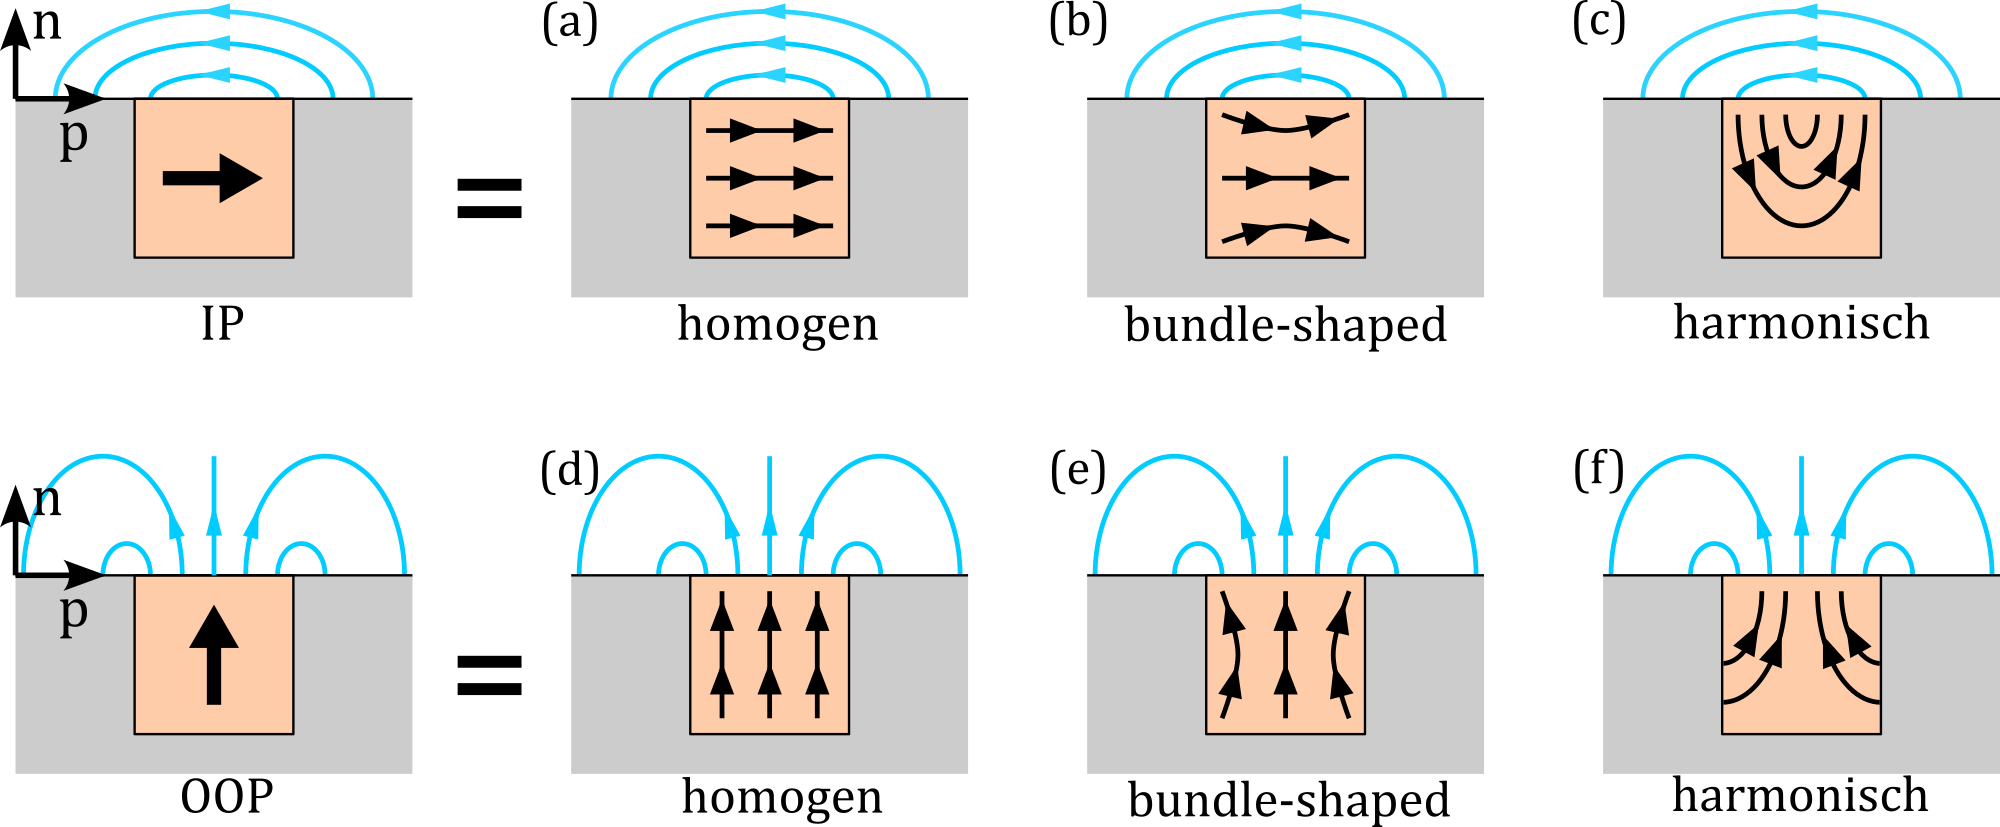
\includegraphics[width=0.9\linewidth,height=\textheight,keepaspectratio]{figures/sec04/02-zone_sketch2.png}

}

\caption{\label{fig-sec04-02-zone_sketch2}IP-Zonen und OOP-Zonen}

\end{figure}%

Abbildung~\ref{fig-sec04-02-zone_sketch2} zeigt schematische Beispiele
für das Magnetfeld (Blau) und die Polarisation (Schwarz) verschiedener
symmetrischer IP- und OOP-Zonen (Orange). Teilbilder (a) und (d) zeigen
homogene Zonen mit gleichmäßiger Polarisation. In der Praxis tritt
jedoch häufig eine „bündelförmige`` (bundle-shaped) Verteilung auf, die
beispielsweise durch magnetostatische Selbstwechselwirkungen entsteht,
siehe (b) und (e). Wird die Polarisation hingegen mit einem Schreibkopf
schrittweise in ein dickes isotropes Material eingeschrieben, entstehen
typischerweise harmonisch verlaufende Muster, wie in (c) und (f)
skizziert. Die dargestellten Fälle verdeutlichen, dass Zonen auch dann
sinnvoll als IP- oder OOP-Zone klassifiziert werden können, wenn die
tatsächliche Polarisation nicht homogen ist.

In vielen Fällen ist die \textbf{Zoneneinteilung nicht eindeutig};
häufig existieren mehrere plausible Möglichkeiten, eine gegebene
Polarisation sinnvoll zu zerlegen. Die gewählte Einteilung sollte daher
stets der praktischen Anwendung, dem Verständnis und der eindeutigen
Kommunikation dienen. In der Praxis ist dies meist bei einer Zerlegung
in IP- oder OOP-Zonen gegeben.

\begin{figure}[h]

\centering{

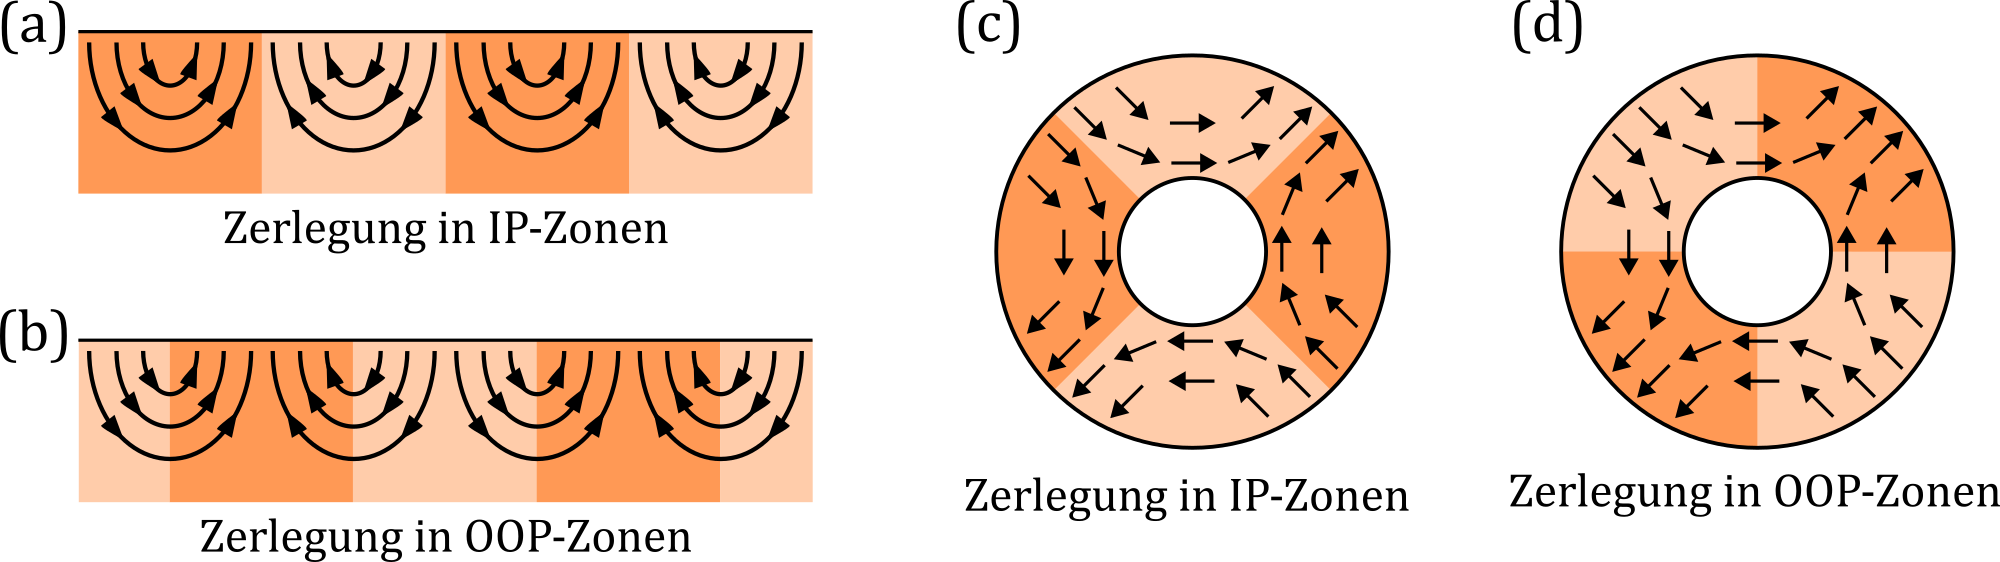
\includegraphics[width=0.9\linewidth,height=\textheight,keepaspectratio]{figures/sec04/03-zone_sketch3.png}

}

\caption{\label{fig-sec04-03-zone_sketch3}Wahl der Zoneneinteilung}

\end{figure}%

In Abbildung~\ref{fig-sec04-03-zone_sketch3} sind Beispiele für
verschiedene sinnvolle Zerlegungen derselben Polarisation skizziert. In
(a) und (b) wird eine harmonische Polarisation einmal in IP-Zonen und
einmal in OOP-Zonen unterteilt. Die Teilbilder (c) und (d) zeigen, dass
auch die Polarisation eines Quadrupolrings sinnvoll sowohl in IP-Zonen
als auch in OOP-Zonen zerlegt werden kann.

\section{Magnetpole}\label{sec-04-magnetpole}

Als \textbf{Magnetpol} wird im allgemeinen Sprachgebrauch ein
Teilbereich der Oberfläche eines magnetisierten Körpers bezeichnet, an
dem das Magnetfeld aus dem Körper austritt oder in ihn eintritt.
Bereiche, an denen das Feld austritt, werden als \textbf{Nordpole}
bezeichnet; Bereiche, an denen es eintritt, als \textbf{Südpole}.

Formal wird hierzu die \textbf{Normalkomponente} des Magnetfeldes an der
Oberfläche des Körpers betrachtet. Ist diese auf der gesamten Oberfläche
bekannt, so kann nach dem Eindeutigkeitssatz der Potentialtheorie das
Streufeld im quellenfreien Außenraum aus ihr eindeutig bestimmt werden
(Jackson 1998).

Für eine \textbf{Poldarstellung} wird die kontinuierliche
Normalkomponente auf der Oberfläche durch einen festgelegten
Schwellenwert auf die Zustände Nord, Null und Süd reduziert. Das
resultierende Polmuster stellt damit eine diskrete Repräsentation der
Normalkomponente dar, aus der sich die Streufeldverteilung qualitativ
ableiten lässt. Der Nutzen der Poldarstellung liegt in einer
anschaulichen qualitativen Beschreibung der Streufeldverteilung eines
Körpers.

\begin{figure}[h]

\centering{

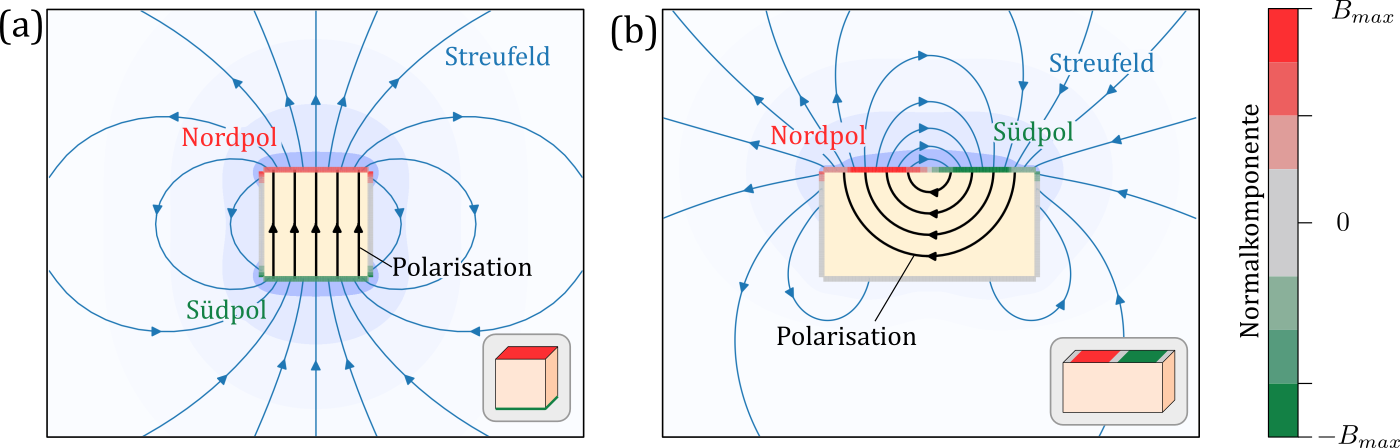
\includegraphics[width=1\linewidth,height=\textheight,keepaspectratio]{figures/sec04/04-magnetpole.png}

}

\caption{\label{fig-sec04-04-magnetpole}Streufeld und Normalkomponente
bei gegebener Polarisation}

\end{figure}%

In Abbildung~\ref{fig-sec04-04-magnetpole} werden das mittels Simulation
ermittelte Streufeld und die Normalkomponente zweier Magnete im
Querschnitt dargestellt. Die Polarisation der Magnete ist in Schwarz
gezeigt. Das Streufeld ist durch Feldlinien sowie durch eine blaue
Farbkontur dargestellt. Die Normalkomponente an der Oberfläche der
Körper ist in einer rot-grau-grünen Farbskala gezeigt.

In (a) ist ein Würfel mit homogener Polarisation simuliert. An seinen
Enden bilden sich die klassischen Polflächen aus. In (b) ist ein Quader
mit inhomogener Polarisation simuliert. Die charakteristischen
Polflächen bilden sich hier einseitig aus. In beiden Teilbildern ist
rechts unten zusätzlich eine repräsentative Nord-Null-Süd-Darstellung
der Magnete gezeigt.

Die in diesem Dokument verwendete feldbezogene Poldefinition ist von der
\textbf{feldtheoretischen Beschreibung} über magnetische Ersatzladungen
zu unterscheiden (Cullity und Graham 2008; Saslow 2022). Bei einfachen
Magneten, insbesondere bei homogen und normal zur Oberfläche
polarisierten Körpern, stimmen beide Beschreibungen häufig
näherungsweise überein. Bei komplexeren Polarisationsverteilungen,
beispielsweise bei IP-Zonenanordnungen, ist diese Übereinstimmung im
Allgemeinen nicht gegeben. Gleiches gilt, wenn die betrachtete
Oberfläche der Maßverkörperung, etwa aufgrund einer Schutzschicht, nicht
mit den Oberflächen der magnetisierten Zonen zusammenfällt. Für
magnetische Maßverkörperungen ist die feldbezogene Definition besonders
zweckmäßig, da sie unmittelbar die anwendungsrelevante
Streufeldverteilung beschreibt.

Da feldbezogene Magnetpole aus der Normalkomponente des Streufeldes
abgeleitet werden, tragen alle Zonen der Maßverkörperung zu ihrer
Ausbildung bei. Pole müssen daher nicht zwingend an den Grenzen
einzelner Zonen liegen. Benachbarte \textbf{Zonen können Polbereiche
verschieben}, verstärken, abschwächen oder sogar auflösen. Ein
anschauliches Beispiel sind Halbach-Anordnungen, bei denen benachbarte
Zonen so ausgerichtet sind, dass die Polausprägung auf einer Seite der
Anordnung verstärkt und auf der gegenüberliegenden Seite abgeschwächt
wird.

\section{Zonenmuster und
Polmuster}\label{sec-04-zonenmuster_und_polmuster}

Die Gesamtheit aller Zonen einer Maßverkörperung wird als
\textbf{Zonenmuster} bezeichnet. Es stellt eine für Kommunikations- und
Referenzierungszwecke geeignete abstrahierte, häufig vereinfachte,
Darstellung der Polarisationsstruktur dar. Die Gesamtheit aller Pole
einer Maßverkörperung wird als \textbf{Polmuster} bezeichnet. Es dient
der qualitativen Beschreibung der Streufeldverteilung. Zonenmuster und
Polmuster sind \textbf{abstrahierte Darstellungen} der magnetischen
Struktur zur anschaulichen und zweckmäßigen Kommunikation.

\begin{figure}[h]

\centering{

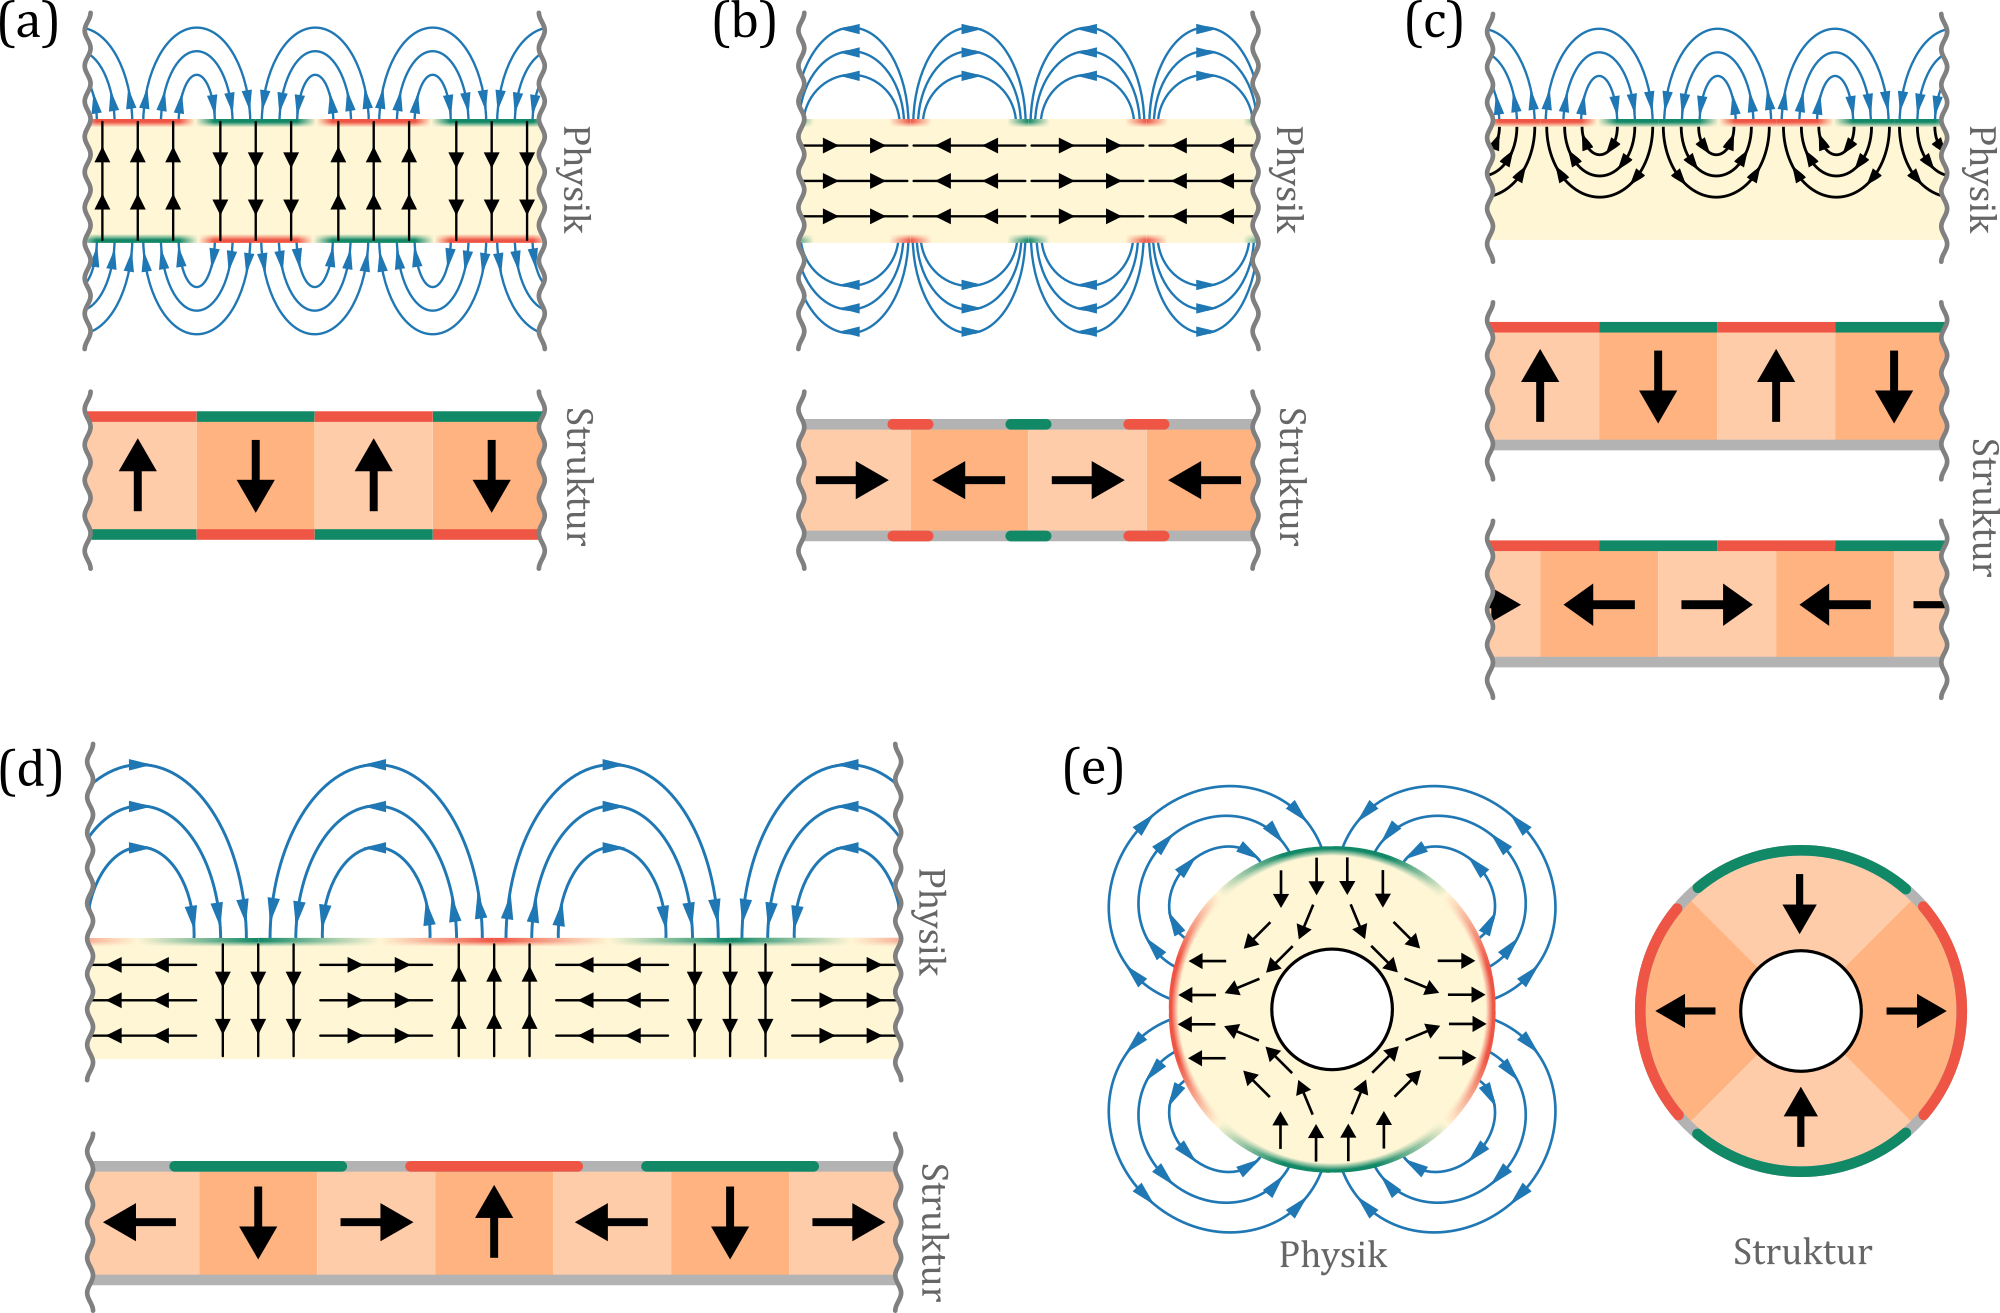
\includegraphics[width=1\linewidth,height=\textheight,keepaspectratio]{figures/sec04/05-magnetische_struktur.png}

}

\caption{\label{fig-sec04-05-magnetische_struktur}Magnetische Struktur
und physikalische Grundlage}

\end{figure}%

Abbildung~\ref{fig-sec04-05-magnetische_struktur} zeigt eine
Gegenüberstellung zwischen der vollständigen physikalischen Beschreibung
(vergleiche mit der Simulation in
Abbildung~\ref{fig-sec04-04-magnetpole}) und den daraus abgeleiteten
Zonen- und Polmustern. Dargestellt sind (a) lineare Anordnung mit
OOP-Polarisationsmuster, (b) lineare Anordnung mit
IP-Polarisationsmuster, (c) lineare Anordnung mit inhomogener
Polarisation, (d) lineare Halbach-Anordnung und (e) ein zylindrischer
Quadrupolmagnet. In Unterbild (c) ist die Zerlegung in Zonen nicht
eindeutig; daher sind beide Möglichkeiten dargestellt. Die Pole befinden
sich jedoch an derselben Stelle.

Polmuster und Zonenmuster sind hier in \textbf{Kombination dargestellt}.
Während das Zonenmuster die Polarisation anschaulich beschreibt, dient
das Polmuster der Veranschaulichung der Streufeldverteilung. Je nach
Zweck kann daher die eine oder die andere Darstellung günstiger sein. So
kann eine Zonenbeschreibung bei komplexer oder in der Tiefe unbekannter
Polarisation schwierig sein, während das Polmuster die wesentliche
Feldverteilung dennoch gut vermittelt.

Ein wichtiges Beispiel sind \textbf{einseitig ausgeprägte Pole}. Diese
können sowohl infolge inhomogener Polarisation wie in (c) und (e), als
auch infolge spezieller Anordnungen, wie in (d), entstehen. Das
Polmuster macht diese einseitige oder zweiseitige Ausprägung unmittelbar
sichtbar, während sie aus dem Zonenmuster häufig nicht direkt ablesbar
ist.

Abschließend sei darauf hingewiesen, dass die Polarisation die
vollständige magnetische Beschreibung der Maßverkörperung bildet. Aus
ihr lassen sich alle anderen Größen ableiten. Umgekehrt lässt sich die
zugrunde liegende Polarisation und damit auch das Zonenmuster aus dem
bekannten Magnetfeld nicht eindeutig rekonstruieren. Dies ist eine Folge
des magnetostatischen inversen Problems (Bruckner u.~a. 2017). In der
Praxis ist die Polarisation jedoch häufig nicht als experimentelle Größe
zugänglich.

\begin{figure}[h]

\centering{

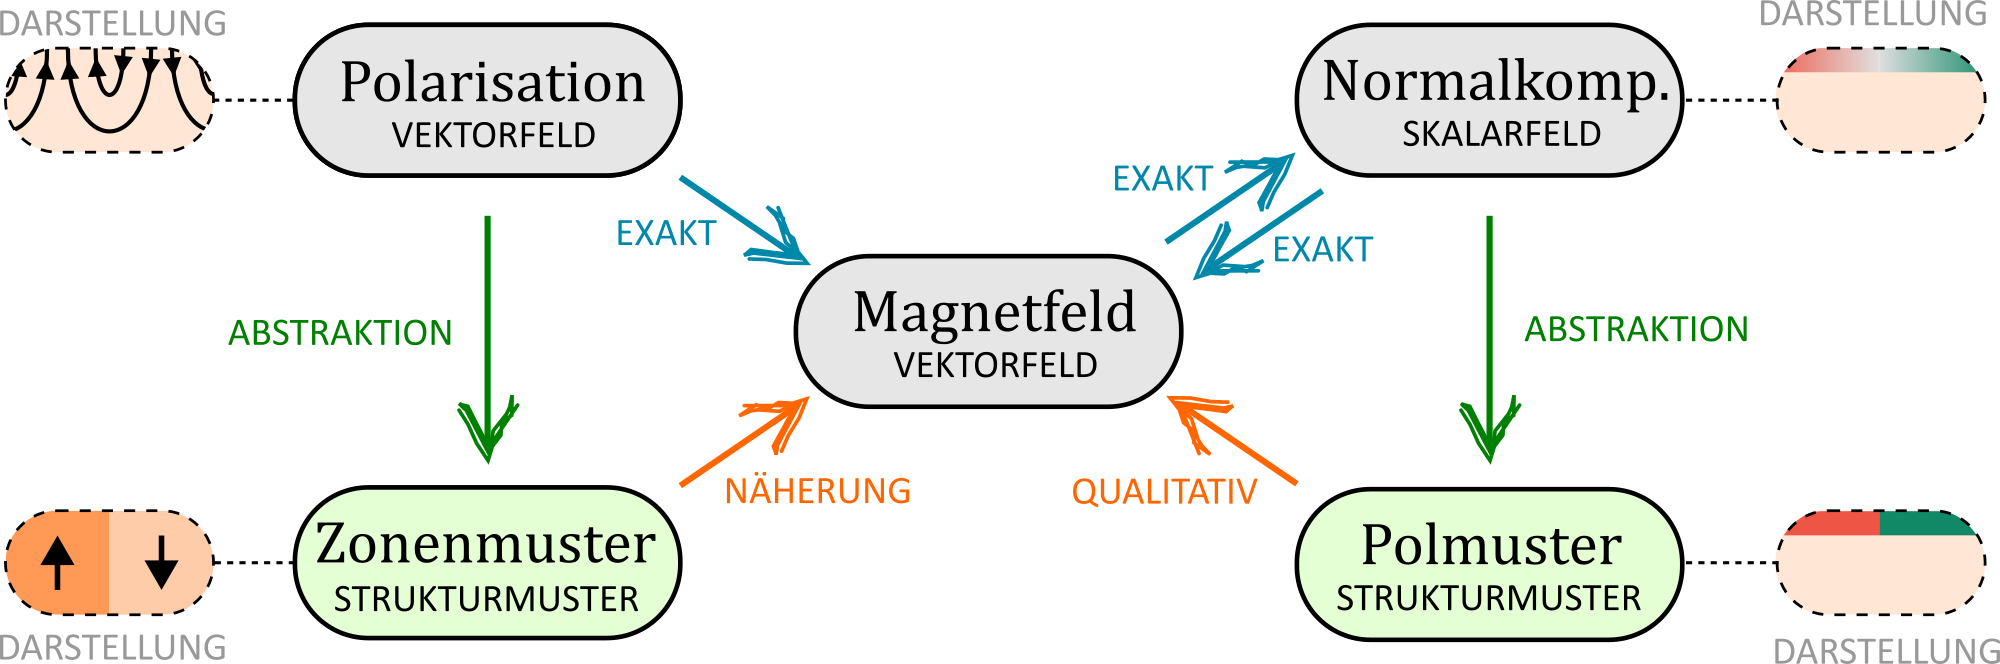
\includegraphics[width=0.9\linewidth,height=\textheight,keepaspectratio]{figures/sec04/06-begriffe_diagramm.png}

}

\caption{\label{fig-sec04-06-begriffe_diagramm}Zusammenhang der
magnetischen Größen}

\end{figure}%

Der Zusammenhang zwischen Polarisation, Magnetfeld, Normalkomponente
sowie den daraus abgeleiteten Zonen- und Polmustern ist in
Abbildung~\ref{fig-sec04-06-begriffe_diagramm} dargestellt. Die Pfeile
geben an, welche Größen jeweils aus welchen anderen Größen abgeleitet
werden können.

\section{Magnetische Spuren}\label{sec-04-magnetische_spuren}

Die magnetische Struktur magnetischer Maßstäbe ist in einem oder
mehreren streifenförmigen Bereichen entlang der funktionalen Oberfläche
angeordnet. Ein solcher Bereich wird als \textbf{magnetische Spur}
bezeichnet. Eine Spur erstreckt sich in \(p\)-Richtung über einen
festgelegten Abschnitt der Maßverkörperung und besitzt eine begrenzte
Ausdehnung in \(o\)-Richtung. Ihr sind alle Zonen und Pole zugeordnet,
die innerhalb ihres Bereichs liegen. Das von einer Spur erzeugte
Magnetfeld wird als \textbf{Spurfeld} bezeichnet.

Die \textbf{Spurausrichtung} richtet sich nach der geometrischen
Anordnung des Messsystems nach
Kapitel~\ref{sec-03-anordnung_des_messsystems}. Entsprechend werden
\textbf{Linearspuren}, \textbf{Radialspuren} und \textbf{Axialspuren}
unterschieden. Linearspuren verlaufen geradlinig entlang der
funktionalen Oberfläche. Radialspuren liegen an einer Innen- oder
Außenmantelfläche einer rotationssymmetrischen Maßverkörperung.
Axialspuren liegen an einer Stirnfläche einer rotationssymmetrischen
Maßverkörperung. Beispielhafte Ausführungen sind in
Abbildung~\ref{fig-sec04-07-spuren_ausrichtung} dargestellt.

\begin{figure}[h]

\centering{

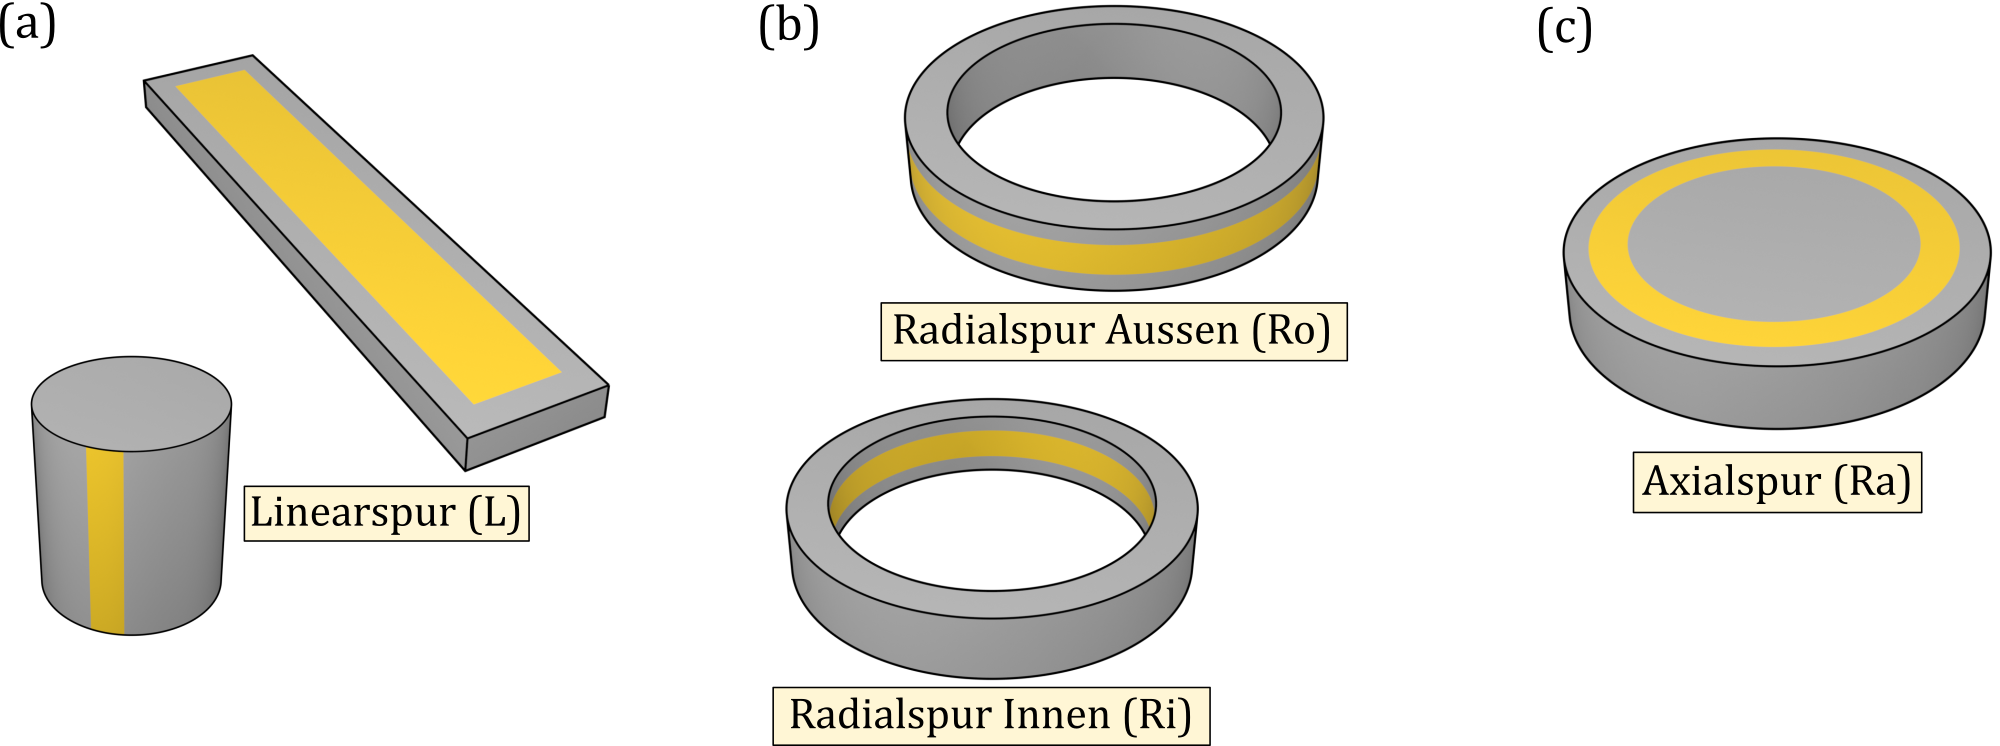
\includegraphics[width=1\linewidth,height=\textheight,keepaspectratio]{figures/sec04/07-spuren_ausrichtung.png}

}

\caption{\label{fig-sec04-07-spuren_ausrichtung}Spurenausrichtung}

\end{figure}%

Der \textbf{Beschreibungsgrad} einer Spur kennzeichnet, in welchem Maß
sie entlang der \(p\)-Richtung magnetisch wirksam beschrieben ist. Eine
Spur ist \textbf{vollbeschrieben}, wenn sie entlang ihrer gesamten Länge
magnetische Zonen aufweist. Eine \textbf{teilbeschriebene} Spur liegt
vor, wenn nur ein begrenzter Abschnitt magnetisch wirksam beschrieben
ist. Ein typisches Beispiel hierfür ist eine Spur mit einem
Referenzbereich. Eine weitere Ausprägung ist die \textbf{segmentiert}
beschriebene Spur, bei der mehrere voneinander getrennte,
aufeinanderfolgende Bereiche magnetisch wirksam beschrieben sind.
Beispielhafte Ausführungen sind in
Abbildung~\ref{fig-sec04-08-beschreibungsgrad} dargestellt.

\begin{figure}[h]

\centering{

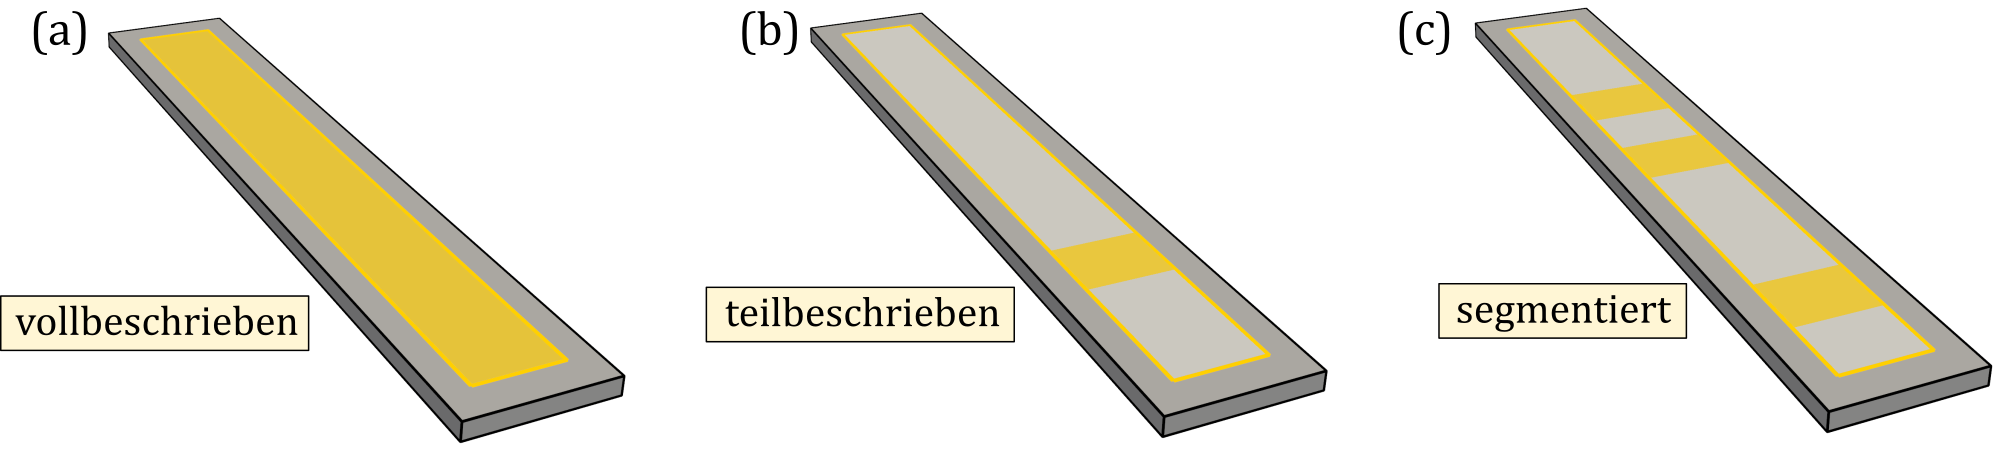
\includegraphics[width=1\linewidth,height=\textheight,keepaspectratio]{figures/sec04/08-beschreibungsgrad.png}

}

\caption{\label{fig-sec04-08-beschreibungsgrad}Beschreibungsgrad einer
Spur}

\end{figure}%

Die \textbf{Polarisationsart einer Spur} ergibt sich aus der
Polarisationsrichtung ihrer Zonen. Besteht die Spur ausschließlich aus
IP-Zonen, spricht man von einer IP-polarisierten Spur oder
\textbf{IP-Spur}. Ist sie ausschließlich aus OOP-Zonen zusammengesetzt,
spricht man von einer OOP-polarisierten Spur oder \textbf{OOP-Spur}.

Einen wichtigen Sonderfall stellt dabei die
\textbf{Halbach-Polarisation} dar. Hier rotiert die
Polarisationsrichtung von Zone zu Zone in der \(p\)-\(n\)-Ebene. Dadurch
entsteht eine asymmetrische Feldverteilung, bei der das Streufeld auf
einer bevorzugten Seite der Maßverkörperung verstärkt wird, während es
auf der gegenüberliegenden Seite weitgehend unterdrückt ist .
Entsprechend spricht man von einer \textbf{Halbach-Spur}.

\section{Darstellungskonventionen}\label{sec-04-darstellungskonventionen}

Dieses Unterkapitel enthält \textbf{Empfehlungen zur Darstellung} von
magnetischen Maßverkörperungen. Es wird durch Ausführungen zur
Felddarstellung in Kapitel~\ref{sec-05-felddarstellung} ergänzt.

Wenn erforderlich, sollte zunächst sichergestellt werden, dass die
\textbf{geometrische Form} einer Maßverkörperung sowie die ihrer
Elemente vollständig erkennbar ist. Hierbei sollten normative Vorgaben,
beispielsweise nach ISO 5456, berücksichtigt werden, in denen zulässige
Projektionsmethoden geometrischer Körper festgelegt sind.

Für die \textbf{Darstellung der Polarisation} (Zonenmuster) sollten
benachbarte Zonen eindeutig unterscheidbar sein. Dies kann
beispielsweise durch Trennlinien, unterschiedliche Füllfarben oder
Schraffuren erreicht werden. Die mittlere Polarisationsrichtung jeder
Zone sollte durch Richtungspfeile gekennzeichnet werden. Vorzugsweise
wird eine Ansicht gewählt, in der die Richtungspfeile unmittelbar auf
den dargestellten Zonenflächen eingetragen und eindeutig räumlich
zugeordnet werden können. Dabei kennzeichnen Pfeile Richtungen parallel
zur Darstellungsebene und die Symbole ⊙ und ⊗ Richtungen senkrecht zur
Darstellungsebene. Kann die Polarisationsrichtung in der gewählten
Ansicht so nicht eindeutig vermittelt werden, können ihre Komponenten in
einer geeigneten orthogonalen Projektion eingezeichnet werden.

\begin{figure}[h]

\centering{

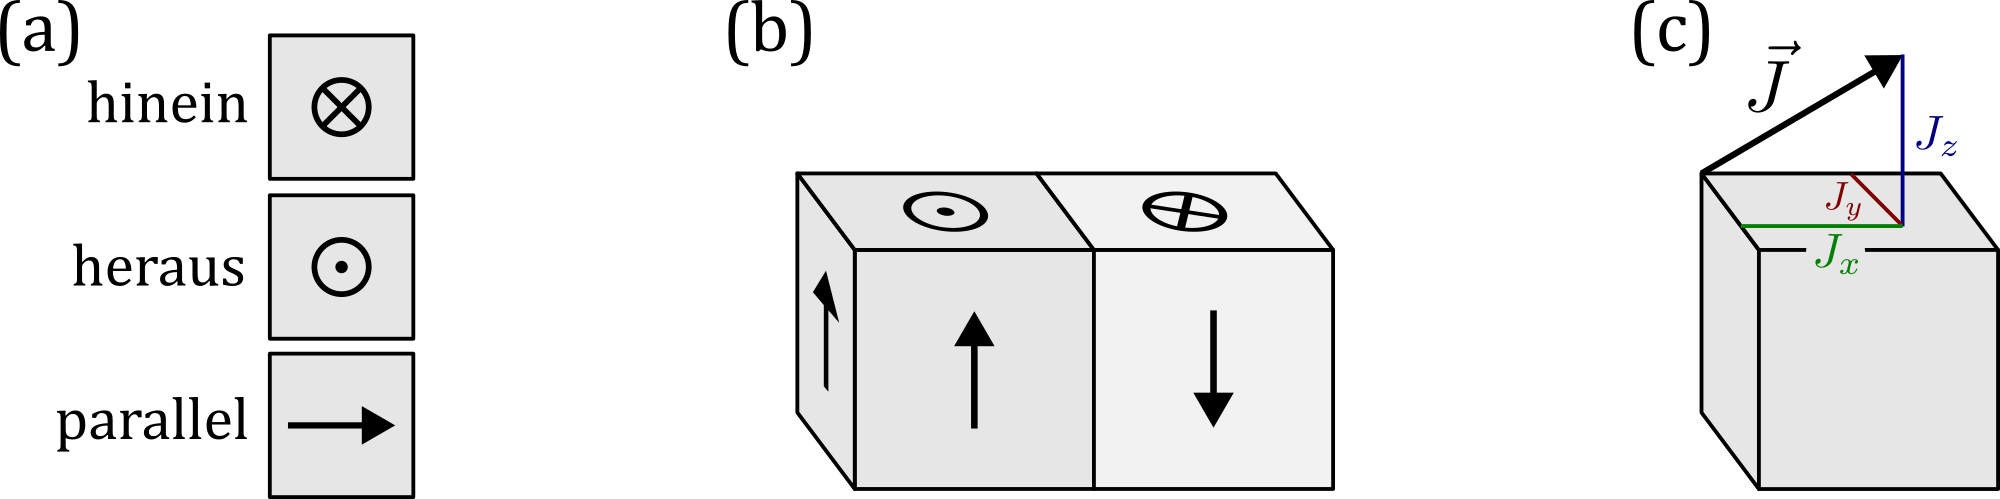
\includegraphics[width=0.7\linewidth,height=\textheight,keepaspectratio]{figures/sec04/09-darstellung_J.png}

}

\caption{\label{fig-sec04-09-darstellung_J}Darstellung der Polarisation}

\end{figure}%

Abbildung~\ref{fig-sec04-09-darstellung_J} (a) zeigt die in diesem
Dokument verwendeten Pfeilsymbole zur Darstellung der
Polarisationsrichtung an Seitenflächen. Teilbild (b) zeigt eine
skizzenhafte Maßverkörperung bestehend aus zwei klar abgegrenzten Zonen
alternierender Polarisation. Teilbild (c) zeigt eine Zone mit nicht
flächenparalleler Polarisation, dargestellt durch Komponenten einer
orthogonalen Projektion auf die Deckfläche.

Zur \textbf{Darstellung des Magnetfeldes} (Normalkomponente, Polmuster,
Felddarstellung) wird der Wert einer ausgewählten Feldkomponente auf
einer Bezugsfläche mittels Rot-Grau-Grün-Farbskala visualisiert. In
Schwarzweißdarstellungen kann entsprechend eine Weiß-Grau-Schwarz-Skala
verwendet werden. Als Bezugsflächen kommen zum Beispiel Zonenseiten,
Körperflächen der Maßverkörperung oder Messflächen in Frage. Die
Farbskala kann je nach Bedarf kontinuierlich oder diskret ausgeführt
werden, wobei binäre und ternäre Ausführungen vor allem für
Poldarstellungen und Felddarstellungen nach
Kapitel~\ref{sec-05-felddarstellung} eingesetzt werden. Besonders bei
diskreten Darstellungen sollte die dargestellte Feldkomponente durch
zusätzliche Richtungssymbole gekennzeichnet werden. Die dafür
verwendeten Symbole unterscheiden sich von den Richtungspfeilen der
Polarisation, um Verwechslung zu vermeiden.

\begin{figure}[h]

\centering{

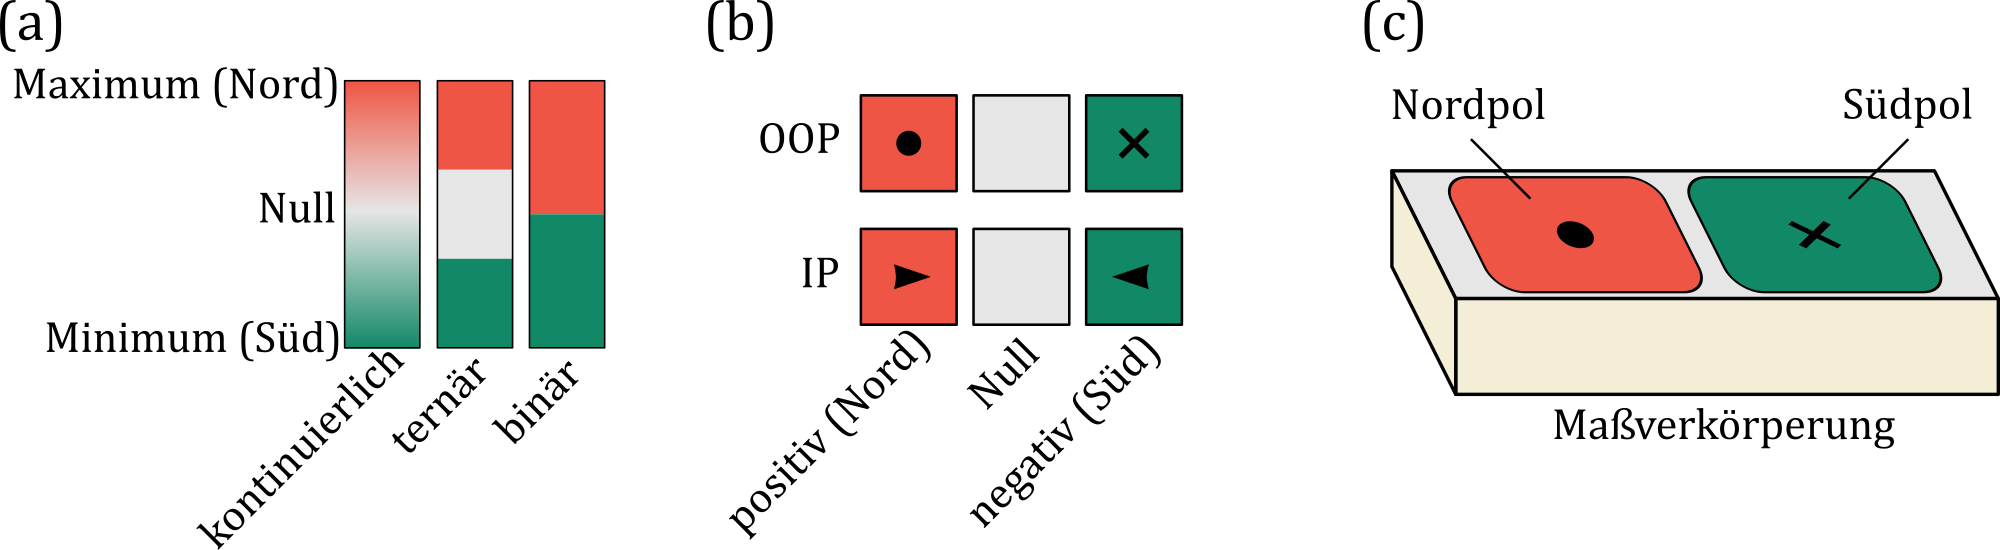
\includegraphics[width=1\linewidth,height=\textheight,keepaspectratio]{figures/sec04/10-darstellung_B.png}

}

\caption{\label{fig-sec04-10-darstellung_B}Darstellung des Magnetfeldes}

\end{figure}%

Abbildung~\ref{fig-sec04-10-darstellung_B} skizziert die Regeln zur
Darstellung des Magnetfeldes. Teilbild (a) zeigt die in diesem Dokument
verwendeten Farbskalen in kontinuierlicher und diskreter Form. Die
eingesetzten Farbcodes sind \#EE5544 für Rot, \#E6E6E6 für Grau und
\#118866 für Grün. Teilbild (b) zeigt die Richtungssymbole zur
Kennzeichnung von IP- und OOP-Komponenten des Magnetfeldes. Teilbild (c)
zeigt beispielhaft eine Maßverkörperung in Poldarstellung. Dabei ist die
auf der Deckfläche ermittelte Normalkomponente mittels dreigeteilter
Farbskala dargestellt.

\begin{tcolorbox}[enhanced jigsaw, arc=.35mm, bottomrule=.15mm, bottomtitle=1mm, breakable, colback=white, colbacktitle=quarto-callout-tip-color!10!white, colframe=quarto-callout-tip-color-frame, coltitle=black, left=2mm, leftrule=.75mm, opacityback=0, opacitybacktitle=0.6, rightrule=.15mm, title=\textcolor{quarto-callout-tip-color}{\faLightbulb}\hspace{0.5em}{Hinweis}, titlerule=0mm, toprule=.15mm, toptitle=1mm]

\emph{In wissenschaftlich-technischen Darstellungen wird die
Farbkombination Rot--Grün üblicherweise vermieden, da sie für viele
Personen mit einer häufig auftretenden Rot-Grün-Sehschwäche nur
eingeschränkt unterscheidbar ist (Crameri u.~a. 2020). In dieser
Richtlinie wird diese Farbwahl jedoch aus historischen Gründen
beibehalten. Die hier gewählten Farben unterscheiden sich deutlich in
Helligkeit und Sättigung, um eine zuverlässige visuelle
Unterscheidbarkeit sicherzustellen.}

\end{tcolorbox}

\begin{figure}[h]

\centering{

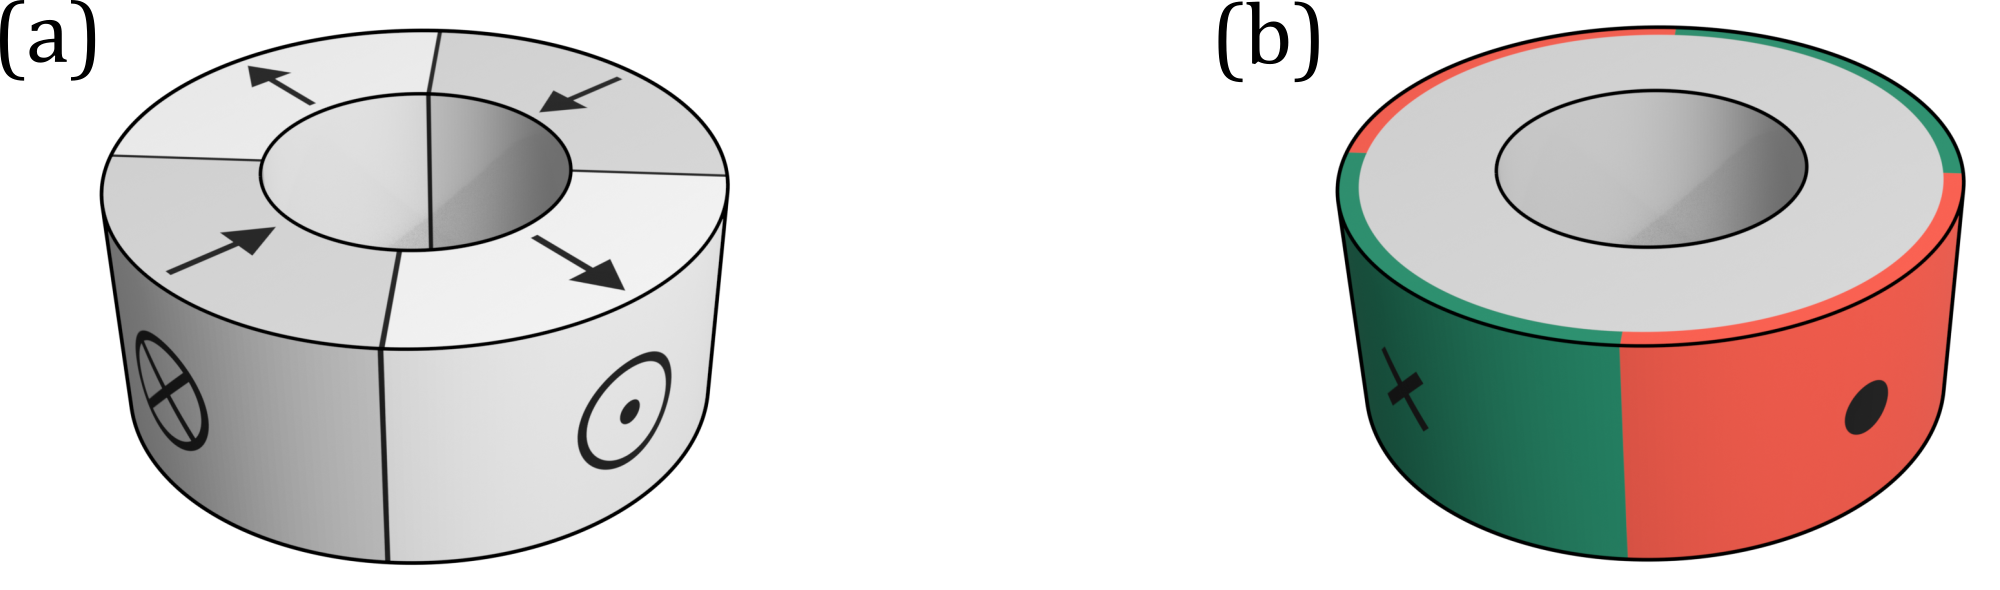
\includegraphics[width=0.75\linewidth,height=\textheight,keepaspectratio]{figures/sec04/11-zonen_und_poldarstellung.png}

}

\caption{\label{fig-sec04-11-zonen_und_poldarstellung}Darstellungsbeispiele
Zonen- und Poldarstellung}

\end{figure}%

Abbildung~\ref{fig-sec04-11-zonen_und_poldarstellung} demonstriert die
beiden Darstellungsformen am Beispiel eines Quadrupolrings, wie er
typischerweise als magnetische Maßverkörperung in radial angeordneten
Winkelmesssystemen mit außen liegenden Sensoren verwendet wird. Die
zugehörige inhomogene Polarisation ist in
Abbildung~\ref{fig-sec04-01-zone_sketch1} (c) skizziert.

Teilbild (a) zeigt den Quadrupolring in Zonendarstellung. Im Vordergrund
steht der strukturelle Aufbau des Magneten, also Anordnung, Form und
Zusammensetzung seiner magnetisierten Zonen.

Teilbild (b) zeigt den Quadrupolring in Poldarstellung. Das Polmuster
ist auf der Mantelfläche binär dargestellt. Es veranschaulicht das nach
außen wirksame Magnetfeld, ohne dabei Information über die innere
magnetische Struktur zu enthalten. Zur besseren Anschaulichkeit wurde
die Farbcodierung über die sichtbare Kante hinweg auf die angrenzende
Deckfläche fortgeführt. Dadurch kann das Polmuster entlang des gesamten
Ringumfangs leichter nachvollzogen werden.

Eine \textbf{kombinierte Darstellung} von Zonen- und Polmuster
ermöglicht es sowohl Polarisationsstruktur als auch Feldwirkung einer
Maßverkörperung zu vermitteln. Das ist besonders bei komplexen
Anordnungen, bei denen sich die Lage der Pole nicht offensichtlich aus
dem Zonenmuster erschließt, hilfreich. Dabei können Pole gegenüber
Zonengrenzen verschoben sein, sich über mehrere Zonen erstrecken oder
sich einseitig ausprägen.

\begin{figure}[h]

\centering{

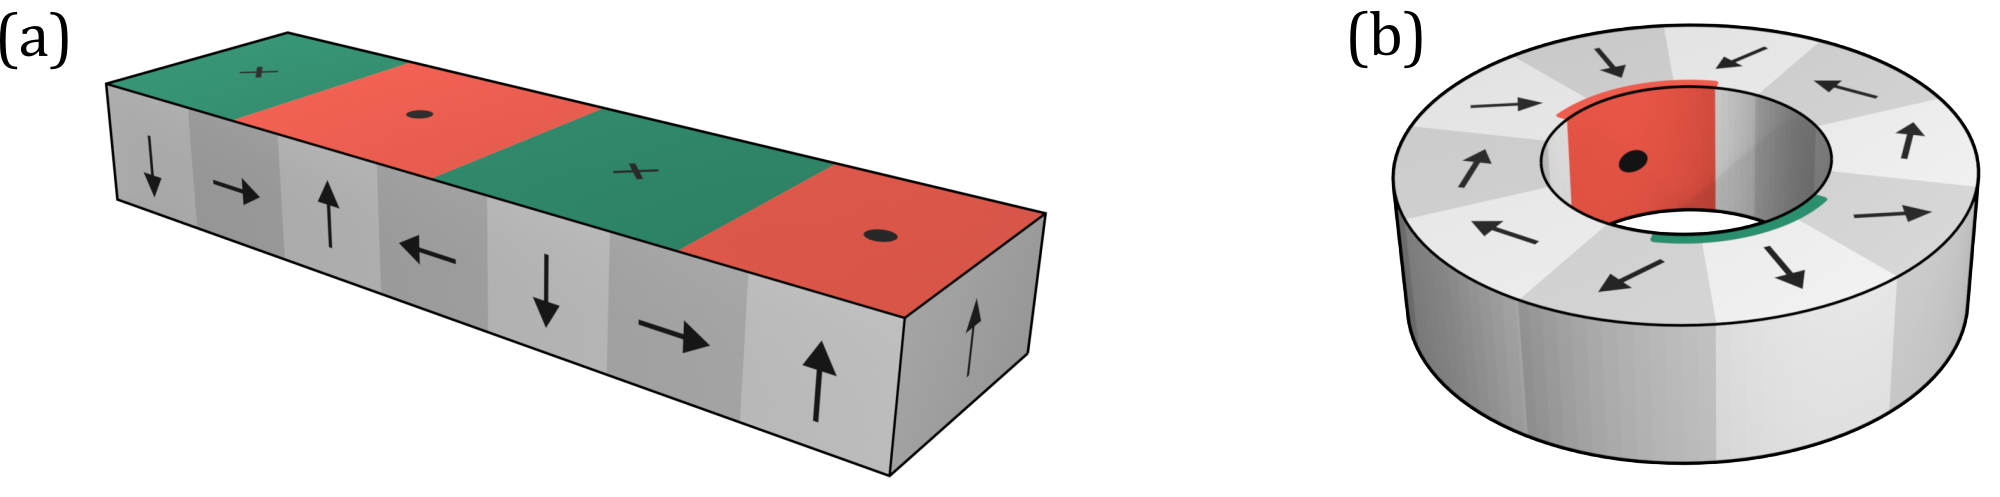
\includegraphics[width=0.9\linewidth,height=\textheight,keepaspectratio]{figures/sec04/12-kombinierte_darstellung.png}

}

\caption{\label{fig-sec04-12-kombinierte_darstellung}Darstellungsbeispiele
kombinierte Darstellung}

\end{figure}%

Abbildung~\ref{fig-sec04-12-kombinierte_darstellung} zeigt zwei
Beispiele solcher kombinierter Darstellungen. Teilbild (a) zeigt einen
Linearmaßstab mit Halbach-Polarisation. Die Pfeile an den Seitenflächen
kennzeichnen das Zonenmuster, während das auf der Oberseite binär
dargestellte Polmuster die daraus resultierende Feldwirkung
veranschaulicht. Teilbild (b) zeigt einen Halbach-Ring. Die Überlagerung
von Zonen- und Polmuster macht die Ausrichtung des Magnetfeldes im
Inneren des Rings unmittelbar erkennbar.

Eine häufig verwendete kombinierte Darstellungsform ist die
\textbf{farbcodierte Zonendarstellung}. Dabei werden die Zonen entlang
ihrer Polarisationsrichtung mit der kontinuierlichen
Magnetfeld-Farbskala eingefärbt. Diese Einfärbung entspricht
näherungsweise der Normalkomponente des Magnetfeldes, die eine isoliert
betrachtete Zone auf ihren Seiten erzeugen würde, wie in
Kapitel~\ref{sec-04-magnetpole} ausgeführt. Bei Zusammensetzung der so
eingefärbten Zonen ergibt sich in vielen Fällen eine anschauliche
Näherung des Polmusters. Voraussetzung ist, dass sich dessen Ausprägung
durch die Überlagerung der Feldbeiträge benachbarter Zonen nicht
wesentlich verändert.

\begin{figure}[h]

\centering{

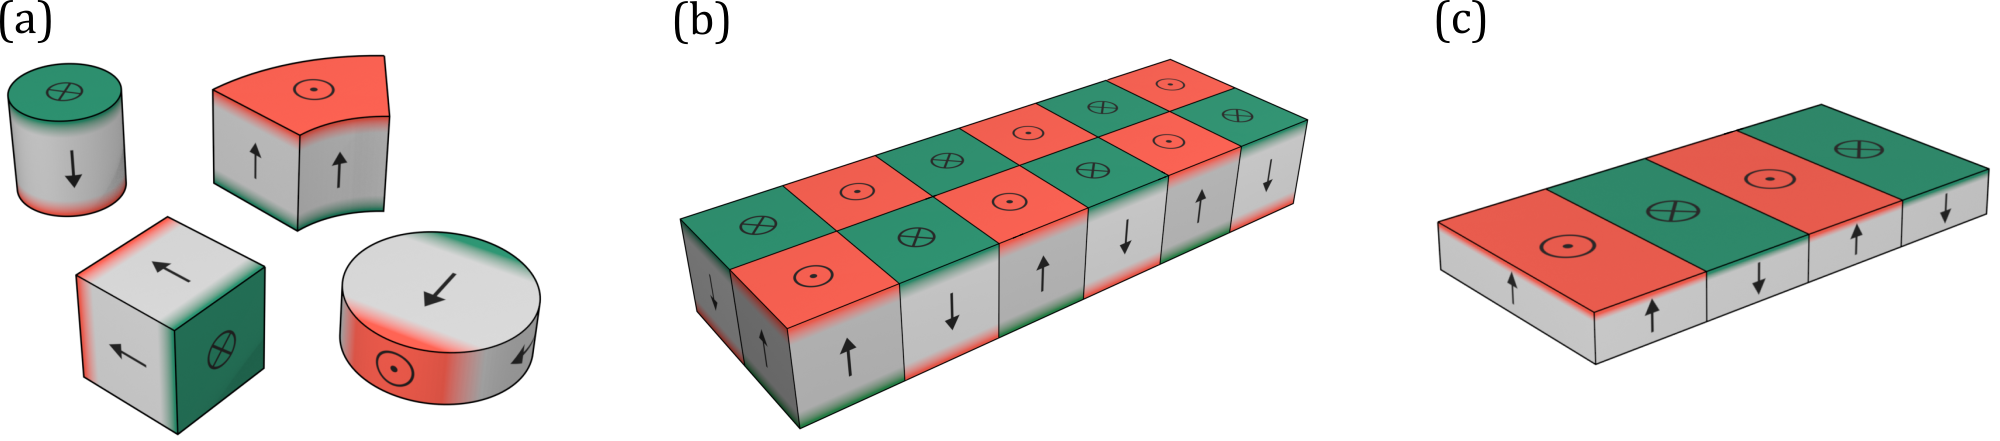
\includegraphics[width=1\linewidth,height=\textheight,keepaspectratio]{figures/sec04/13-farbcodierte_zonendarstellung.png}

}

\caption{\label{fig-sec04-13-farbcodierte_zonendarstellung}Darstellungsbeispiele
farbcodierte Zonendarstellung}

\end{figure}%

Abbildung~\ref{fig-sec04-13-farbcodierte_zonendarstellung} demonstriert
die farbcodierte Zonendarstellung anhand verschiedener Beispiele.
Teilbild (a) zeigt unterschiedliche Dipolmagnete, deren erwartete
Feldwirkung durch die Einfärbung der Körperflächen hervorgehoben wird.
Teilbild (b) zeigt zweireihig axial gestapelte Würfelmagnete. Die
einzelnen Zonen sind klar voneinander abgegrenzt; ihre Einfärbung
veranschaulicht das auf Ober- und Unterseite erwartete Polmuster.
Teilbild (c) zeigt, wie mit der farbcodierten Zonendarstellung eine
einseitige Ausprägung der Pole vermittelt werden kann. Die mögliche
zugrunde liegende inhomogene Polarisationsverteilung wird in den
Kapitel~\ref{sec-04-magnetisierte_zonen} und
Kapitel~\ref{sec-04-magnetpole} näher beschrieben.

\begin{tcolorbox}[enhanced jigsaw, arc=.35mm, bottomrule=.15mm, bottomtitle=1mm, breakable, colback=white, colbacktitle=quarto-callout-tip-color!10!white, colframe=quarto-callout-tip-color-frame, coltitle=black, left=2mm, leftrule=.75mm, opacityback=0, opacitybacktitle=0.6, rightrule=.15mm, title=\textcolor{quarto-callout-tip-color}{\faLightbulb}\hspace{0.5em}{Hinweis}, titlerule=0mm, toprule=.15mm, toptitle=1mm]

\emph{Weicht das resultierende Polmuster deutlich von der Zonenstruktur
ab, wie bei den Beispielen in
Abbildung~\ref{fig-sec04-12-kombinierte_darstellung}, ist die
farbcodierte Zonendarstellung ungeeignet und kann zu
\textbf{irreführenden Farbzuordnungen} führen.}

\emph{Aufgrund ihrer großen \textbf{Ähnlichkeit zur Poldarstellung}
besteht zudem eine erhöhte Verwechslungsgefahr. Daher sollte stets
eindeutig angegeben werden, welche Darstellungsform verwendet wird.}

\end{tcolorbox}

Spuren können bei Bedarf durch eine \textbf{Umrahmung} und durch die
Hervorhebung nichtmagnetisierter Bereiche gekennzeichnet werden. Die
Kennzeichnung ermöglicht die eindeutige Zuordnung der zugehörigen Zonen
und Pole und verdeutlicht, ob sich eine Spur auch über
nichtmagnetisierte Abschnitte erstreckt.

\begin{figure}[h]

\centering{

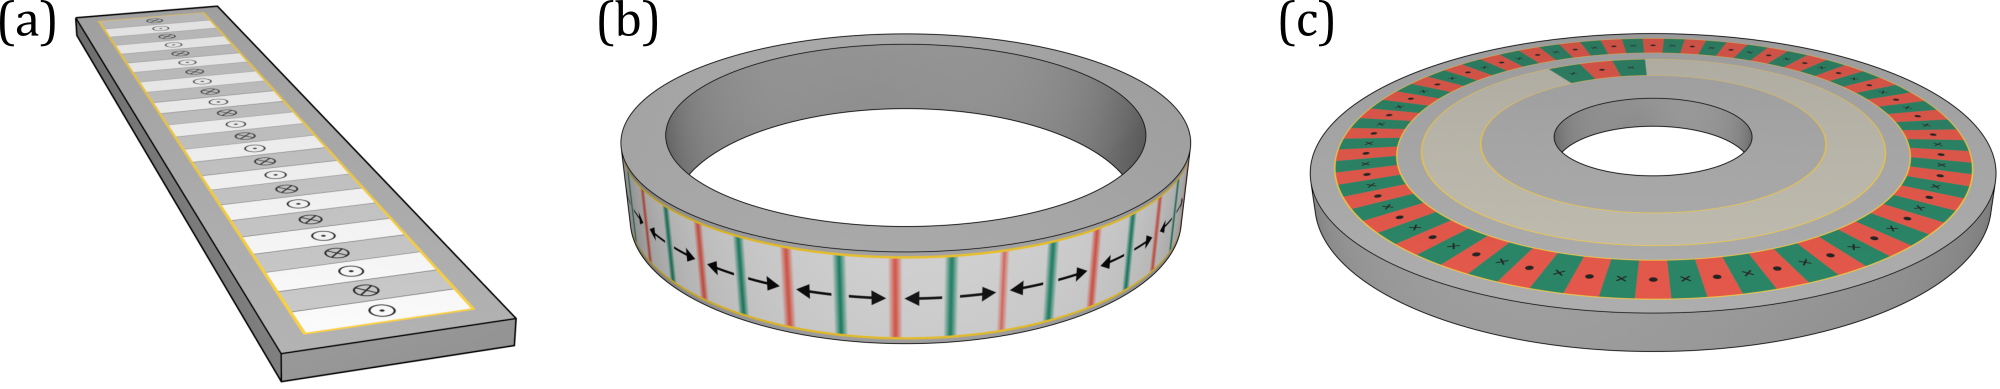
\includegraphics[width=1\linewidth,height=\textheight,keepaspectratio]{figures/sec04/14-darstellung_spuren.png}

}

\caption{\label{fig-sec04-14-darstellung_spuren}Darstellungsbeispiele
Spuren}

\end{figure}%

Abbildung~\ref{fig-sec04-14-darstellung_spuren} zeigt drei exemplarische
Darstellungen magnetischer Maßstäbe. Teilbild (a) zeigt einen typischen
Linearmaßstab zur Positionserfassung von Linearachsen. Er weist eine
inkrementelle OOP-Spur auf, die in reiner Zonendarstellung gezeigt ist.
Teilbild (b) zeigt einen Rotationsmaßstab mit einer radial außen
liegenden inkrementellen IP-Spur in farbcodierter Zonendarstellung.
Derartige Maßverkörperungen werden häufig in Drehgebern eingesetzt.
Teilbild (c) zeigt einen Rotationsmaßstab mit zwei axial angeordneten
Spuren in Poldarstellung. Die äußere Spur ist eine vollbeschriebene
Inkrementalspur. Die innere Spur ist eine teilbeschriebene Spur mit
Referenzpolen. Eine solche Kombination wird oft zur absoluten
Positionserfassung eingesetzt.

\section{Magnetische
Struktur}\label{sec-04-magnetische_strukturbeschreibung}

Bisher wurde die magnetische Struktur einer Maßverkörperung anhand von
Zonen, Polen und Spuren qualitativ beschrieben. Im Folgenden werden
Strukturbegriffe festgelegt, die eine eindeutige geometrische und
technisch detaillierte Beschreibung dieser Strukturelemente ermöglichen.

\subsection{Struktur-KS und
Begrenzungsbox-Geometrie}\label{sec-04-strukturKS}

Die Beschreibung der magnetischen Struktur erfolgt in einem zweckmäßig
gewählten \textbf{Struktur-KS} mit Ursprung \(O_T\). Seine
Koordinatenrichtungen sind in der Regel an den \(p\)-, \(o\)- und
\(n\)-Richtungen des Maßverkörperungs-KS ausgerichtet.

Ist das Struktur-KS einer magnetischen Spur zugeordnet, wird es als
\textbf{Spur-KS} bezeichnet; der Ursprung wird weiterhin mit \(O_T\)
bezeichnet. Besitzt ein magnetischer Maßstab mehrere Spuren, sollte
jeder Spur ein eigenes Spur-KS zugeordnet werden.

Als zweckmäßige \textbf{Konvention} wird empfohlen, den Ursprung \(O_T\)
in \(o\)-Richtung mittig zur beschriebenen magnetischen Struktur und in
\(n\)-Richtung auf der funktionalen Oberfläche der Maßverkörperung
anzuordnen. Die \(p\)-Lage wird anhand eines eindeutig festgelegten
Strukturbezugs gewählt, typischerweise am Beginn der ersten genutzten
Zone oder des ersten genutzten Pols. Bei einem Spur-KS wird hierfür
vorzugsweise der Beginn der Spur verwendet.

\begin{figure}[h]

\centering{

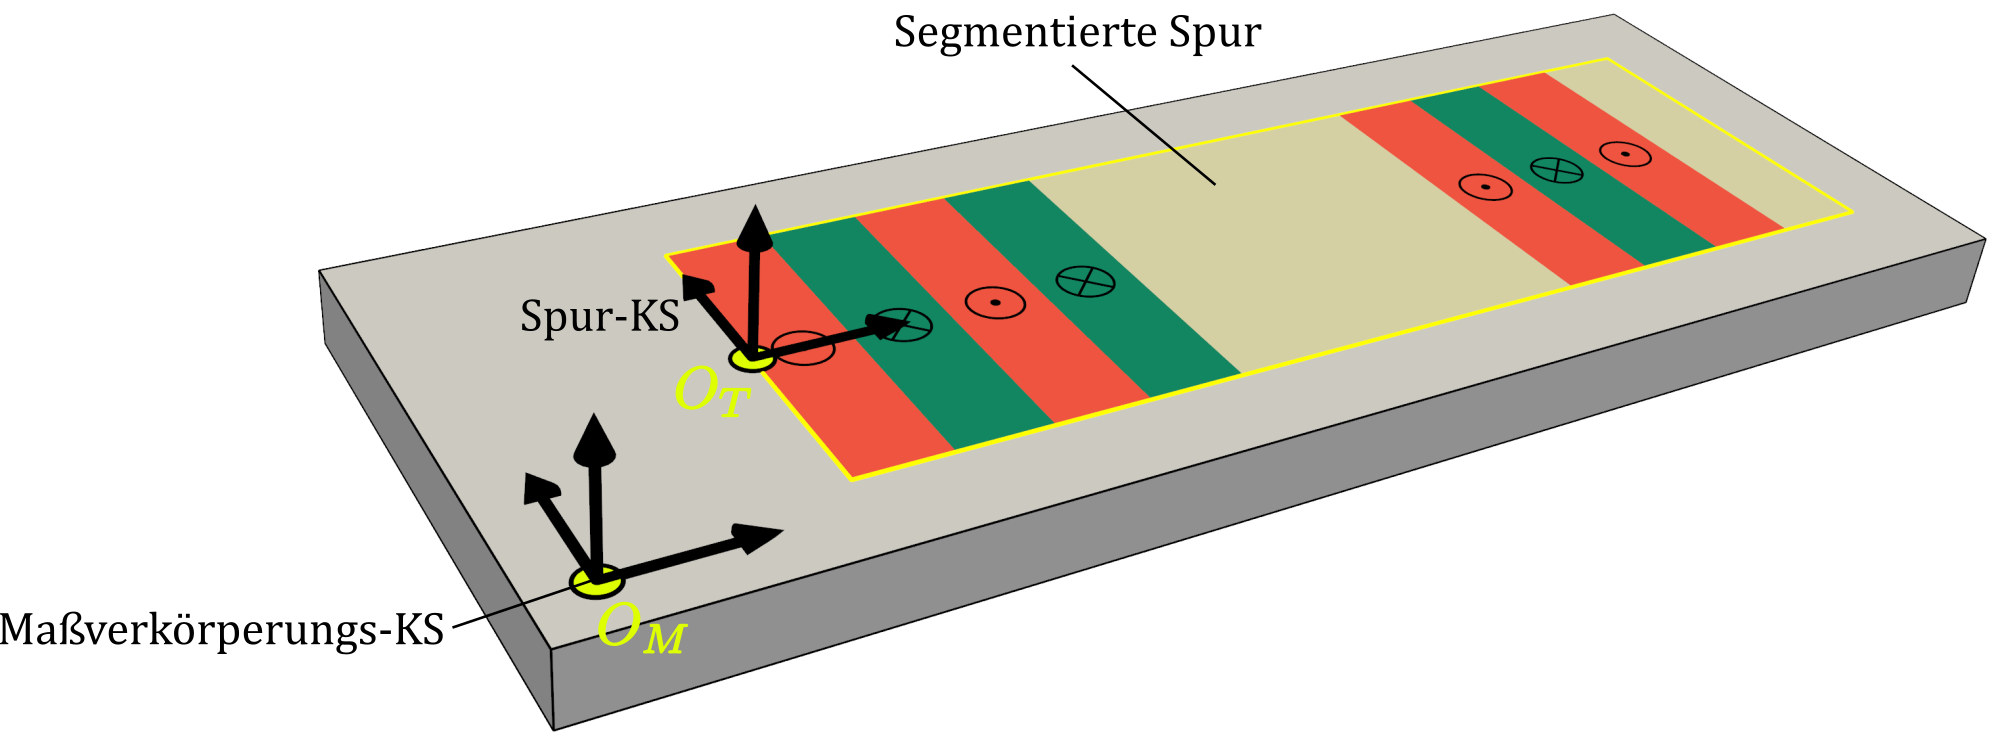
\includegraphics[width=0.9\linewidth,height=\textheight,keepaspectratio]{figures/sec04/15-spurKS.png}

}

\caption{\label{fig-sec04-15-spurKS}Struktur-KS am Beispiel einer
magnetischen Spur}

\end{figure}%

Abbildung~\ref{fig-sec04-15-spurKS} veranschaulicht die Festlegung eines
Struktur-KS. Entsprechend der Konvention liegt dessen Ursprung in
\(o\)-Richtung mittig zur magnetischen Struktur, in \(p\)-Richtung am
Beginn der magnetischen Struktur und in \(n\)-Richtung auf der
funktionalen Oberfläche der Maßverkörperung.

Lage und Abmessungen magnetisierter Zonen, von Magnetpolen und
magnetischen Spuren können in vielen Fällen näherungsweise durch
\textbf{Begrenzungsboxkörper} erfasst werden. In kartesischen
Koordinaten sind dies achsenparallele Quader, bei zylindrischer
Koordinatendarstellung Zylinder- oder Ringsegmente. Angaben in
\(p\)-Richtung können dabei nach Kapitel~\ref{sec-03} als Länge oder
Winkel angegeben werden.

\begin{tcolorbox}[enhanced jigsaw, arc=.35mm, bottomrule=.15mm, bottomtitle=1mm, breakable, colback=white, colbacktitle=quarto-callout-tip-color!10!white, colframe=quarto-callout-tip-color-frame, coltitle=black, left=2mm, leftrule=.75mm, opacityback=0, opacitybacktitle=0.6, rightrule=.15mm, title=\textcolor{quarto-callout-tip-color}{\faLightbulb}\hspace{0.5em}{Hinweis}, titlerule=0mm, toprule=.15mm, toptitle=1mm]

\emph{Die nachfolgenden Strukturbegriffe werden verwendet, soweit sich
die magnetische Struktur mit der zugrunde liegenden
Begrenzungsbox-Geometrie zweckmäßig beschreiben lässt. Für andere
Geometrien sind geeignete alternative Größen zu verwenden, wie
beispielhaft in Abbildung~\ref{fig-sec04-17-struktur_mp_ring} gezeigt.}

\end{tcolorbox}

\subsection{Strukturbegriffe magnetisierter
Zonen}\label{sec-04-strukturbegriffe_zonen}

In Begrenzungsbox-Geometrien werden die Abmessungen magnetisierter Zonen
in \(p\)-Richtung durch die \textbf{Zonenlänge} \(\ell_Z\), in
\(o\)-Richtung durch die \textbf{Zonenbreite} \(w_Z\) und in
\(n\)-Richtung durch die \textbf{Zonentiefe} \(d_Z\) beschrieben.

Zonen werden zu Referenzierungszwecken aufsteigend in positiver
\(p\)-Richtung mit dem Ordnungsindex \(j=1,…,N_Z\) nummeriert. Die
\textbf{Zonenanzahl} \(N_Z\) bezeichnet die Gesamtzahl der nummerierten
Zonen. Eine vollständige Indizierung aller vorhandenen Zonen ist nicht
erforderlich.

Auf eine Zone kann in \(p\)-Richtung ein Zwischenraum folgen, der keiner
Zone zugeordnet ist. Solch ein Zwischenraum entsteht beispielsweise bei
aus einzelnen Dipolmagneten zusammengesetzten Maßverkörperungen. Die
Ausdehnung des Zwischenraums in \(p\)-Richtung wird als
\textbf{Zonenspalt} \(\bar{\ell}_Z^{(j)}\) bezeichnet. Er trägt den
gleichen Index wie die vorangehende Zone.

Die \textbf{Zonenlage} \(\vec{r}_Z\) bezeichnet die Position des
geometrischen Mittelpunkts des Begrenzungsboxkörpers. Ihre Koordinaten
sind \(p_Z\), \(o_Z\) und \(n_Z\).

\begin{figure}[h]

\centering{

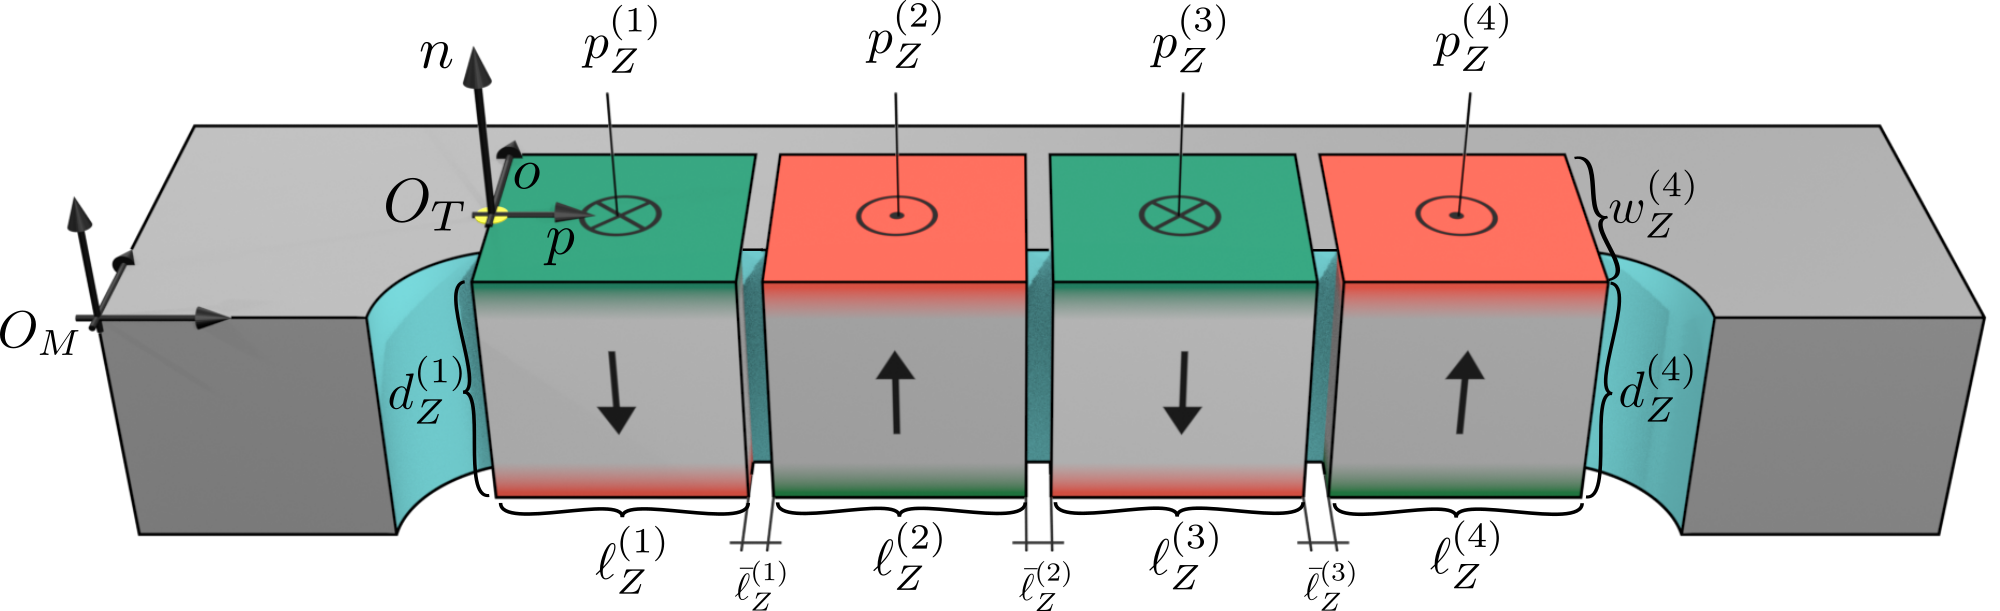
\includegraphics[width=0.9\linewidth,height=\textheight,keepaspectratio]{figures/sec04/16-struktur_mp_quader.png}

}

\caption{\label{fig-sec04-16-struktur_mp_quader}Strukturbeschreibung des
Zonenmusters eines Multipolquaders}

\end{figure}%

Abbildung~\ref{fig-sec04-16-struktur_mp_quader} zeigt eine beispielhafte
Strukturbeschreibung einer magnetischen Maßverkörperung mittels Zonen in
kartesischen Koordinaten. Die Maßverkörperung besteht aus einer
Halterung mit vier eingesetzten würfelförmigen Dipolmagneten, die in
einem OOP-Muster angeordnet sind. Die Halterung ist zur besseren
Sichtbarkeit teilweise aufgeschnitten dargestellt. Jeder Dipolmagnet
wird dabei als eine Zone aufgefasst. Die Zonen sind in positiver
\(p\)-Richtung nummeriert und zugeordnete Größen mit einem
entsprechenden Ordnungsindex versehen. Der Ursprung des Struktur-KS
\(O_T\) liegt entsprechend der Konvention in \(o\)-Richtung mittig zur
Zonenstruktur, in \(n\)-Richtung auf der funktionalen Oberfläche der
Maßverkörperung und in \(p\)-Richtung am Beginn der ersten Zone.

\begin{figure}[h]

\centering{

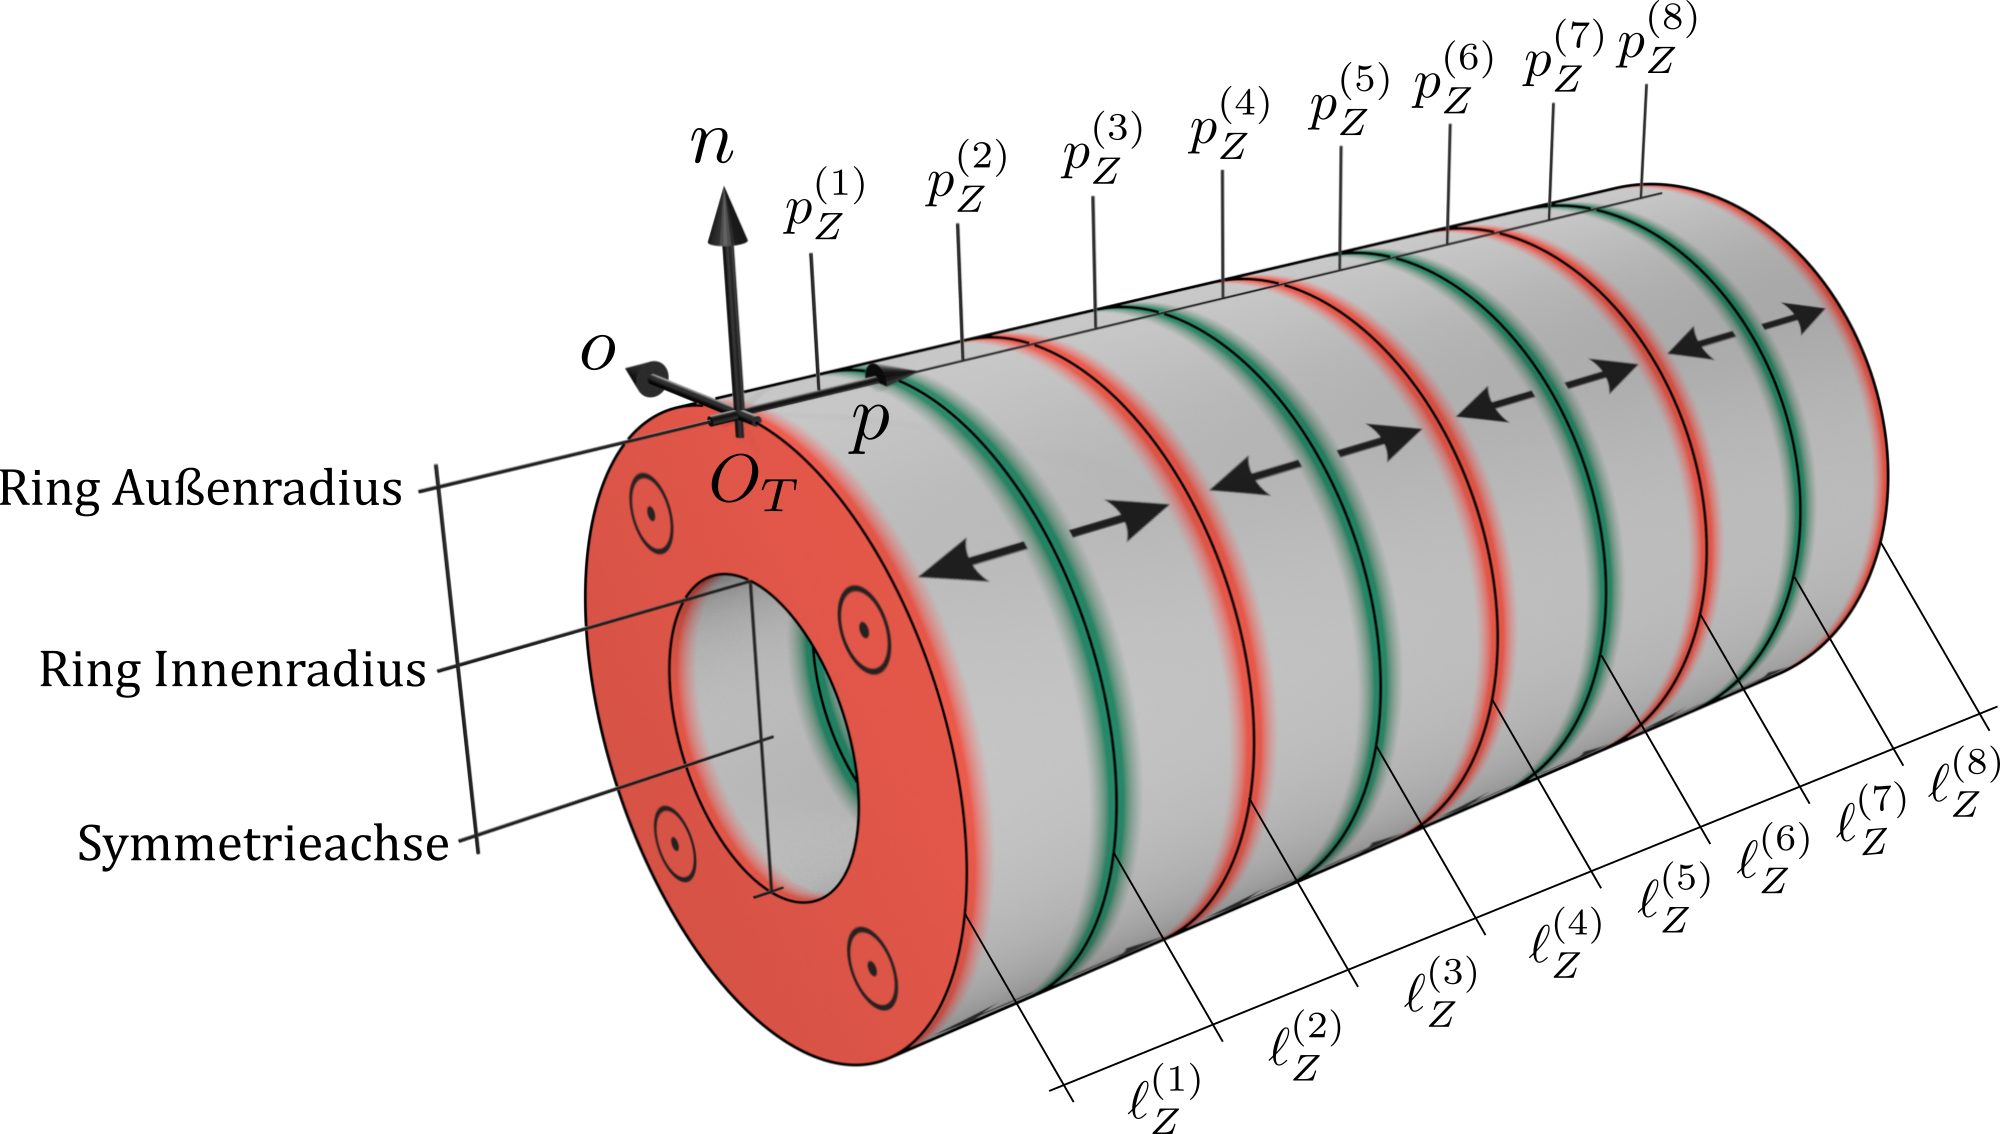
\includegraphics[width=0.8\linewidth,height=\textheight,keepaspectratio]{figures/sec04/17-struktur_mp_ring.png}

}

\caption{\label{fig-sec04-17-struktur_mp_ring}Strukturbeschreibung des
Zonenmusters eines axialen Multipolrings}

\end{figure}%

In Abbildung~\ref{fig-sec04-17-struktur_mp_ring} ist das Zonenmuster
eines axial gestapelten Multipolrings mit \(N_Z=8\) dargestellt.
Derartige Maßverkörperungen können zur Detektion axialer Verschiebungen
entlang der Systemachse eingesetzt werden. Der Ursprung des Struktur-KS
ist auf der Mantelfläche in \(o\)-Richtung mittig und in \(p\)-Richtung
am Beginn der ersten Zone festgelegt.

Obwohl die Maßverkörperung ringförmig ist, handelt es sich dabei um eine
lineare Anordnung. In diesem Beispiel ist der Begriff der Zonenlänge
sinnvoll anwendbar, da die Zonen entlang der \(p\)-Richtung gestapelt
sind. Die Begriffe Zonenbreite und Zonentiefe sind aufgrund der
ringförmigen Geometrie hingegen nicht zweckmäßig. Zur Beschreibung der
Geometrie der Maßverkörperung werden stattdessen Innen- und Außenradius
des Rings genutzt.

\begingroup
\footnotesize
\renewcommand{\baselinestretch}{1.12}\selectfont
\setlength{\tabcolsep}{5pt}
\setlength{\extrarowheight}{2.5pt}
\renewcommand{\arraystretch}{1.15}
{\begin{longtable}[]{
  >{\raggedright\arraybackslash}p{(\linewidth - 4\tabcolsep) * \real{0.2500}}
  >{\centering\arraybackslash}p{(\linewidth - 4\tabcolsep) * \real{0.1500}}
  >{\raggedright\arraybackslash}p{(\linewidth - 4\tabcolsep) * \real{0.6000}}}
\caption{Begriffe Zonen}\label{tbl-begriffe_zonen}\tabularnewline
\arrayrulecolor{tableouterrule}
\toprule\noalign{}
\rowcolor{zebrabluehead}
\begin{minipage}[b]{\linewidth}\raggedright
\textbf{Begriff}
\end{minipage} & \begin{minipage}[b]{\linewidth}\centering
\textbf{Symbol}
\end{minipage} & \begin{minipage}[b]{\linewidth}\raggedright
\textbf{Beschreibung}
\end{minipage} \\
\arrayrulecolor{tableheadrule}
\specialrule{0.35pt}{0pt}{0pt}
\endhead
\arrayrulecolor{tableouterrule}
\specialrule{0.30pt}{0pt}{0pt}
\endlastfoot
\rowcolor{zebrabluelight}
\textbf{Zonenanzahl} & \(N_Z\) & Gesamtzahl der nummerierten Zonen \\
\arrayrulecolor{tableline}
\specialrule{0.15pt}{0pt}{0pt}
\rowcolor{zebrabluedark}
\textbf{Zonenlänge} & \(\ell_Z^{(j)}\) & Ausdehnung der Zone \(j\) in
\(p\)-Richtung \\
\arrayrulecolor{tableline}
\specialrule{0.15pt}{0pt}{0pt}
\rowcolor{zebrabluelight}
\textbf{Zonenbreite} & \(w_Z^{(j)}\) & Ausdehnung der Zone \(j\) in
\(o\)-Richtung \\
\arrayrulecolor{tableline}
\specialrule{0.15pt}{0pt}{0pt}
\rowcolor{zebrabluedark}
\textbf{Zonentiefe} & \(d_Z^{(j)}\) & Ausdehnung der Zone \(j\) in
\(n\)-Richtung \\
\arrayrulecolor{tableline}
\specialrule{0.15pt}{0pt}{0pt}
\rowcolor{zebrabluelight}
\textbf{Zonenspalt} & \(\bar{\ell}_Z^{(j)}\) & Ausdehnung des einer Zone
\(j\) folgenden, keiner Zone zugeordneten Zwischenraums in
\(p\)-Richtung \\
\arrayrulecolor{tableline}
\specialrule{0.15pt}{0pt}{0pt}
\rowcolor{zebrabluedark}
\textbf{Zonenlage} & \(\vec{r}_Z^{(j)}\) & Position des geometrischen
Mittelpunkts des Begrenzungsboxkörpers der Zone \(j\); Koordinaten
\(p_Z^{(j)}\), \(o_Z^{(j)}\) und \(n_Z^{(j)}\) \\
\arrayrulecolor{tableline}
\specialrule{0.15pt}{0pt}{0pt}
\end{longtable}
}
\endgroup

\subsection{Strukturbegriffe magnetischer
Pole}\label{sec-04-strukturbegriffe_pole}

In Begrenzungsbox-Geometrien werden die Abmessungen von Magnetpolen in
\(p\)-Richtung durch die \textbf{Pollänge} \(\ell_P\) und in
\(o\)-Richtung durch die \textbf{Polbreite} \(w_P\) beschrieben.

Pole werden zu Referenzierungszwecken aufsteigend in positiver
\(p\)-Richtung mit dem Ordnungsindex \(j = 1, \ldots, N_P\) nummeriert.
Die \textbf{Polanzahl} \(N_P\) bezeichnet die Gesamtzahl der
nummerierten Pole. Eine vollständige Indizierung aller vorhandenen Pole
ist nicht erforderlich.

Die \textbf{Pollage} \(\vec{r}_P\) bezeichnet die Position des
geometrischen Mittelpunkts der Begrenzungsbox. Ihre Koordinaten sind
\(p_P\) und \(o_P\).

\begin{figure}[h]

\centering{

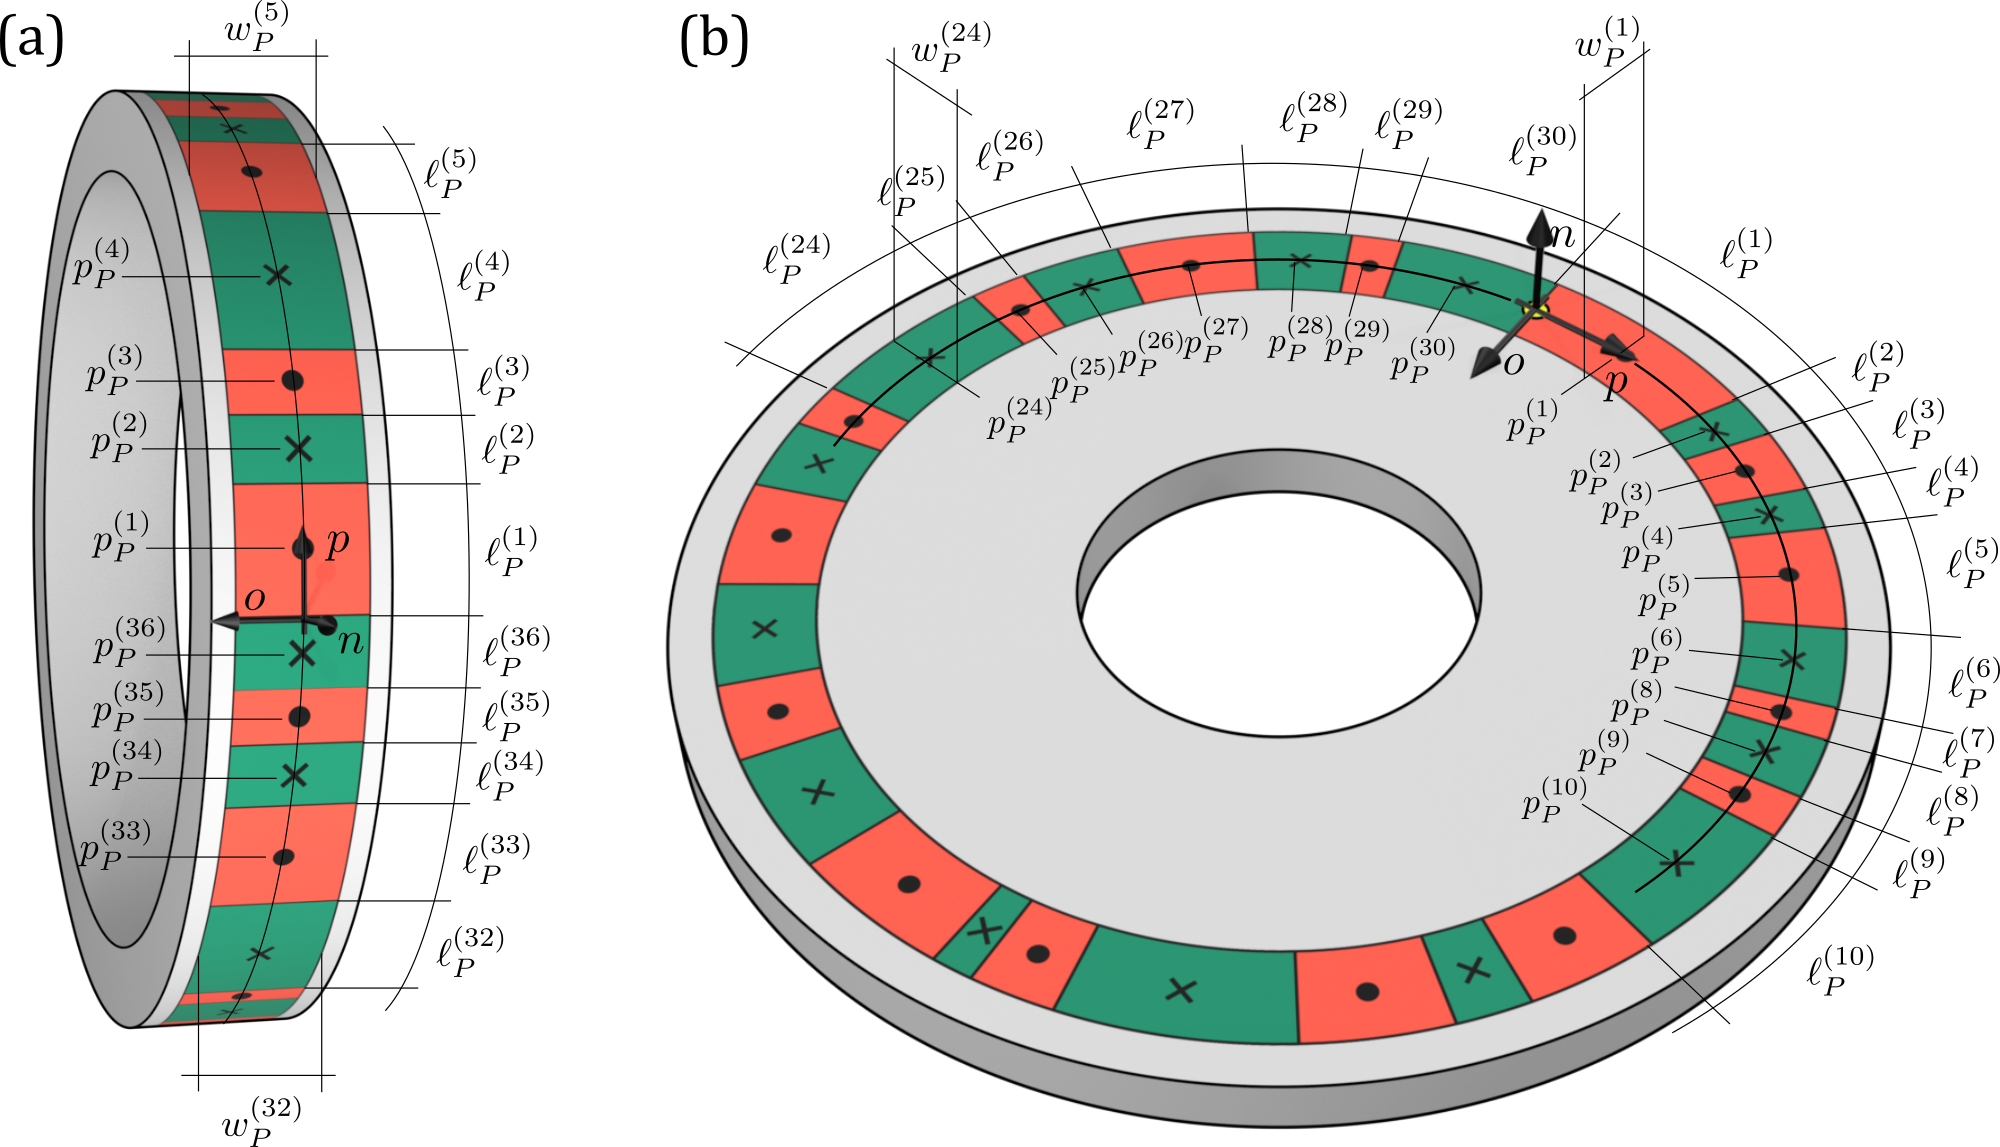
\includegraphics[width=1\linewidth,height=\textheight,keepaspectratio]{figures/sec04/18-struktur_pole.png}

}

\caption{\label{fig-sec04-18-struktur_pole}Strukturbeschreibung des
Polmusters}

\end{figure}%

Abbildung~\ref{fig-sec04-18-struktur_pole} zeigt eine beispielhafte
Strukturbeschreibung von Polmustern in zylindrischen
Begrenzungsbox-Geometrien. Dargestellt sind zwei Polräder mit
Pseudo-Random-Codierung. In Teilbild (a) ist eine außenliegende
Radialspur mit \(N_P = 36\) nummerierten Polen gezeigt; in Teilbild (b)
eine Axialspur mit \(N_P = 30\) nummerierten Polen. Bei radial
außenliegenden Spuren wie in Teilbild (a) ist es zweckmäßig, \(p_P\) und
\(\ell_P\) als Bogenlängen anzugeben. Bei der Axialspur in Teilbild (b)
ist dies aufgrund des über die Spurbreite veränderlichen Radius hingegen
nicht zweckmäßig.

\begingroup
\footnotesize
\renewcommand{\baselinestretch}{1.12}\selectfont
\setlength{\tabcolsep}{5pt}
\setlength{\extrarowheight}{2.5pt}
\renewcommand{\arraystretch}{1.15}
{\begin{longtable}[]{
  >{\raggedright\arraybackslash}p{(\linewidth - 4\tabcolsep) * \real{0.2500}}
  >{\centering\arraybackslash}p{(\linewidth - 4\tabcolsep) * \real{0.1500}}
  >{\raggedright\arraybackslash}p{(\linewidth - 4\tabcolsep) * \real{0.6000}}}
\caption{Begriffe Pole}\label{tbl-begriffe_pole}\tabularnewline
\arrayrulecolor{tableouterrule}
\toprule\noalign{}
\rowcolor{zebrabluehead}
\begin{minipage}[b]{\linewidth}\raggedright
\textbf{Begriff}
\end{minipage} & \begin{minipage}[b]{\linewidth}\centering
\textbf{Symbol}
\end{minipage} & \begin{minipage}[b]{\linewidth}\raggedright
\textbf{Beschreibung}
\end{minipage} \\
\arrayrulecolor{tableheadrule}
\specialrule{0.35pt}{0pt}{0pt}
\endhead
\arrayrulecolor{tableouterrule}
\specialrule{0.30pt}{0pt}{0pt}
\endlastfoot
\rowcolor{zebrabluelight}
\textbf{Polanzahl} & \(N_P\) & Gesamtzahl der nummerierten Pole \\
\arrayrulecolor{tableline}
\specialrule{0.15pt}{0pt}{0pt}
\rowcolor{zebrabluedark}
\textbf{Pollänge} & \(\ell_P^{(j)}\) & Ausdehnung des Pols \(j\) in
\(p\)-Richtung \\
\arrayrulecolor{tableline}
\specialrule{0.15pt}{0pt}{0pt}
\rowcolor{zebrabluelight}
\textbf{Polbreite} & \(w_P^{(j)}\) & Ausdehnung des Pols \(j\) in
\(o\)-Richtung \\
\arrayrulecolor{tableline}
\specialrule{0.15pt}{0pt}{0pt}
\rowcolor{zebrabluedark}
\textbf{Pollage} & \(\vec{r}_P^{(j)}\) & Position des geometrischen
Mittelpunkts der Begrenzungsbox des Pols \(j\); Koordinaten
\(p_P^{(j)}\) und \(o_P^{(j)}\) \\
\arrayrulecolor{tableline}
\specialrule{0.15pt}{0pt}{0pt}
\end{longtable}
}
\endgroup

\subsection{Strukturbegriffe magnetischer
Spuren}\label{sec-04-strukturbegriffe_spuren}

In Begrenzungsbox-Geometrien werden die Abmessungen magnetischer Spuren
in \(p\)-Richtung durch die \textbf{Spurlänge} \(\ell_T\), in
\(o\)-Richtung durch die \textbf{Spurbreite} \(w_T\) und in
\(n\)-Richtung durch die \textbf{Spurtiefe} \(d_T\) beschrieben.

Spuren werden zu Referenzierungszwecken mit dem Ordnungsindex
\(i = 1, \ldots, N_T\) nummeriert. Bei parallel angeordneten Spuren
erfolgt die Nummerierung aufsteigend in positiver \(o\)-Richtung. Die
\textbf{Spuranzahl} \(N_T\) bezeichnet die Gesamtzahl der nummerierten
Spuren.

Die \textbf{Spurlage} \(\vec{r}_T\) bezeichnet die Position des
Spur-KS-Ursprungs \(O_T\) im Maßverkörperungs-KS. Ihre Koordinaten sind
\(p_T\), \(o_T\) und \(n_T\). Mit der üblichen Festlegung von \(O_T\)
auf der funktionalen Oberfläche der Maßverkörperung gilt \(n_T = 0\).

Die relative Lage zweier Spuren wird durch ihre Versätze beschrieben.
Der \textbf{Spur-Längsversatz} \(p_{TT}\), auch
\textbf{Spur-\(p\)-Versatz}, bezeichnet den Versatz in \(p\)-Richtung.
Für die Spuren mit den Ordnungsindizes \(i_1\) und \(i_2\) gilt:

\[
p_{TT}^{(i_1,i_2)} = p_T^{(i_2)} - p_T^{(i_1)}.
\]

Der \textbf{Spur-Querversatz} \(o_{TT}\), auch
\textbf{Spur-\(o\)-Versatz}, bezeichnet entsprechend den Versatz in
\(o\)-Richtung:

\[
o_{TT}^{(i_1,i_2)} = o_T^{(i_2)} - o_T^{(i_1)}.
\]

Für Größen, die sich auf zwei Spuren beziehen, wird nach
Kapitel~\ref{sec-03-indexkonvention} der Bezugsindex „TT`` verwendet.
Der \textbf{Spurabstand} \(w_{TT}\) bezeichnet den Abstand in
\(o\)-Richtung zwischen zwei benachbarten Spuren.

\begin{figure}[h]

\centering{

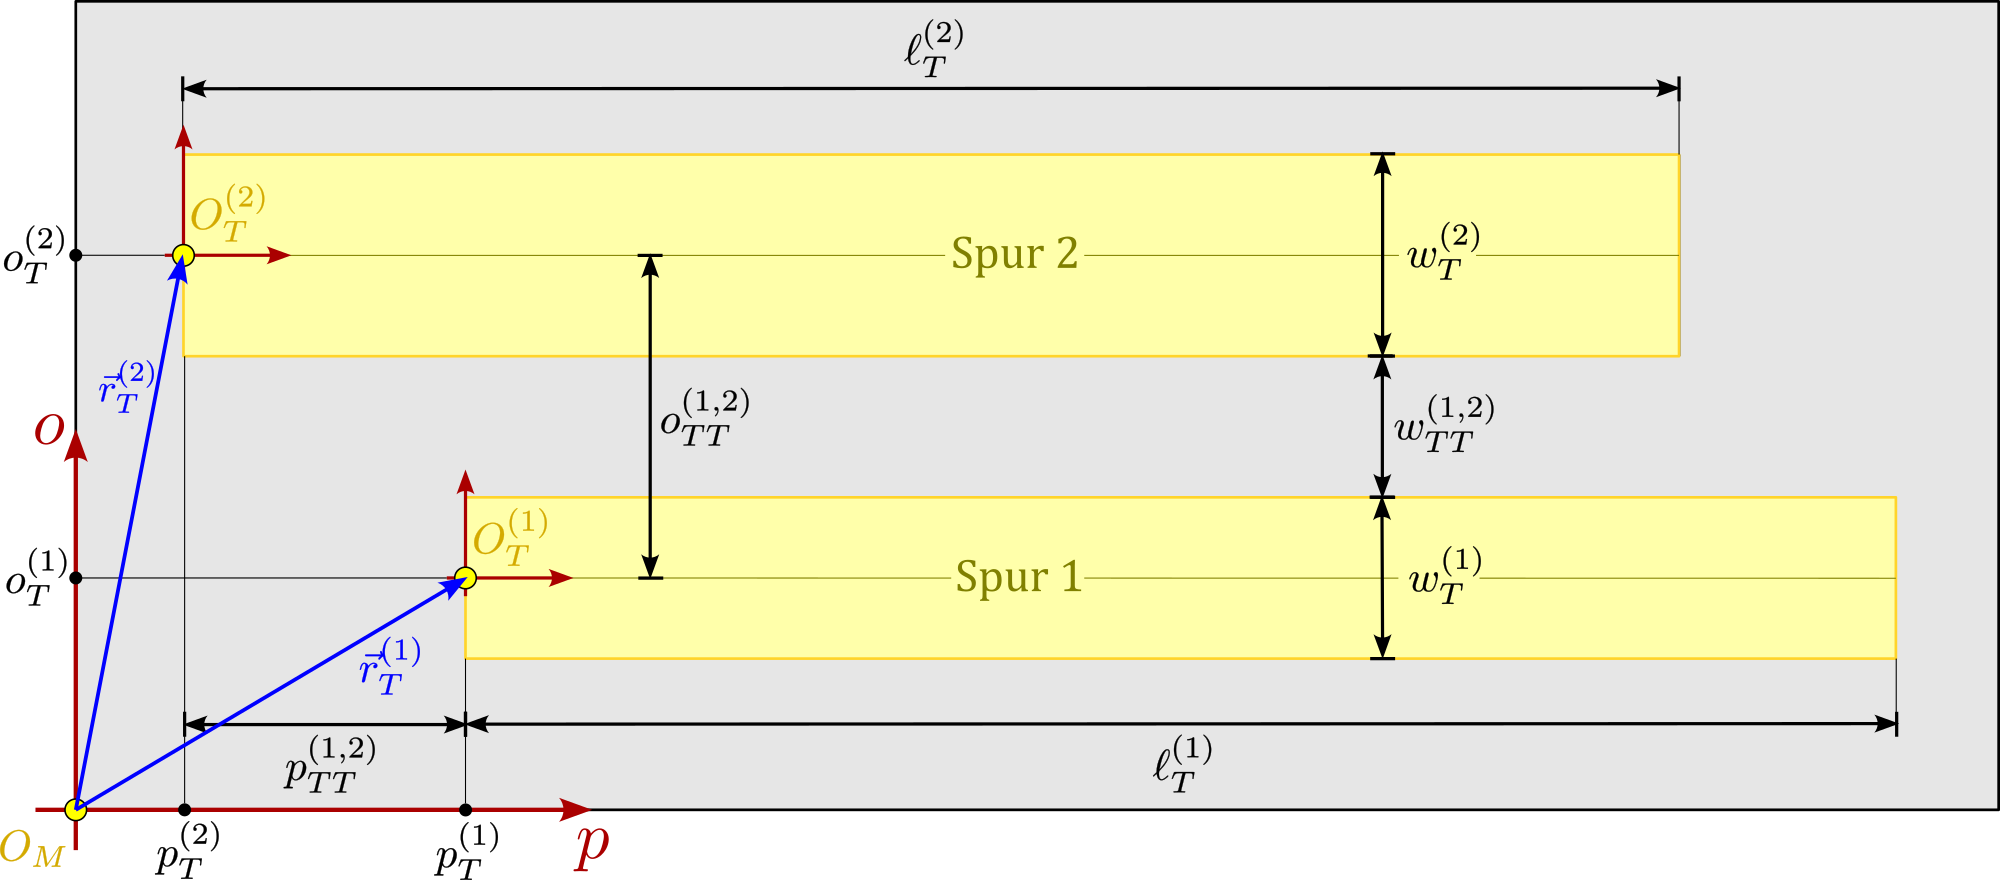
\includegraphics[width=1\linewidth,height=\textheight,keepaspectratio]{figures/sec04/19-struktur_spuren.png}

}

\caption{\label{fig-sec04-19-struktur_spuren}Strukturbeschreibung von
magnetischen Spuren}

\end{figure}%

Abbildung~\ref{fig-sec04-19-struktur_spuren} veranschaulicht die
eingeführten Spurbegriffe anhand einer schematischen Darstellung eines
magnetischen Maßstabs mit zwei parallelen Linearspuren, die gelb
hervorgehoben sind. Die Ursprünge der Spur-KS sind entsprechend der
eingeführten Konvention in \(p\)-Richtung am Beginn der jeweiligen Spur
und mittig in \(o\)-Richtung festgelegt. Die relevanten Spurgrößen,
insbesondere Spurlage, Spurabmessungen, Spurversätze und Spurabstand,
sind in der Abbildung eingezeichnet.

\begin{figure}[h]

\centering{

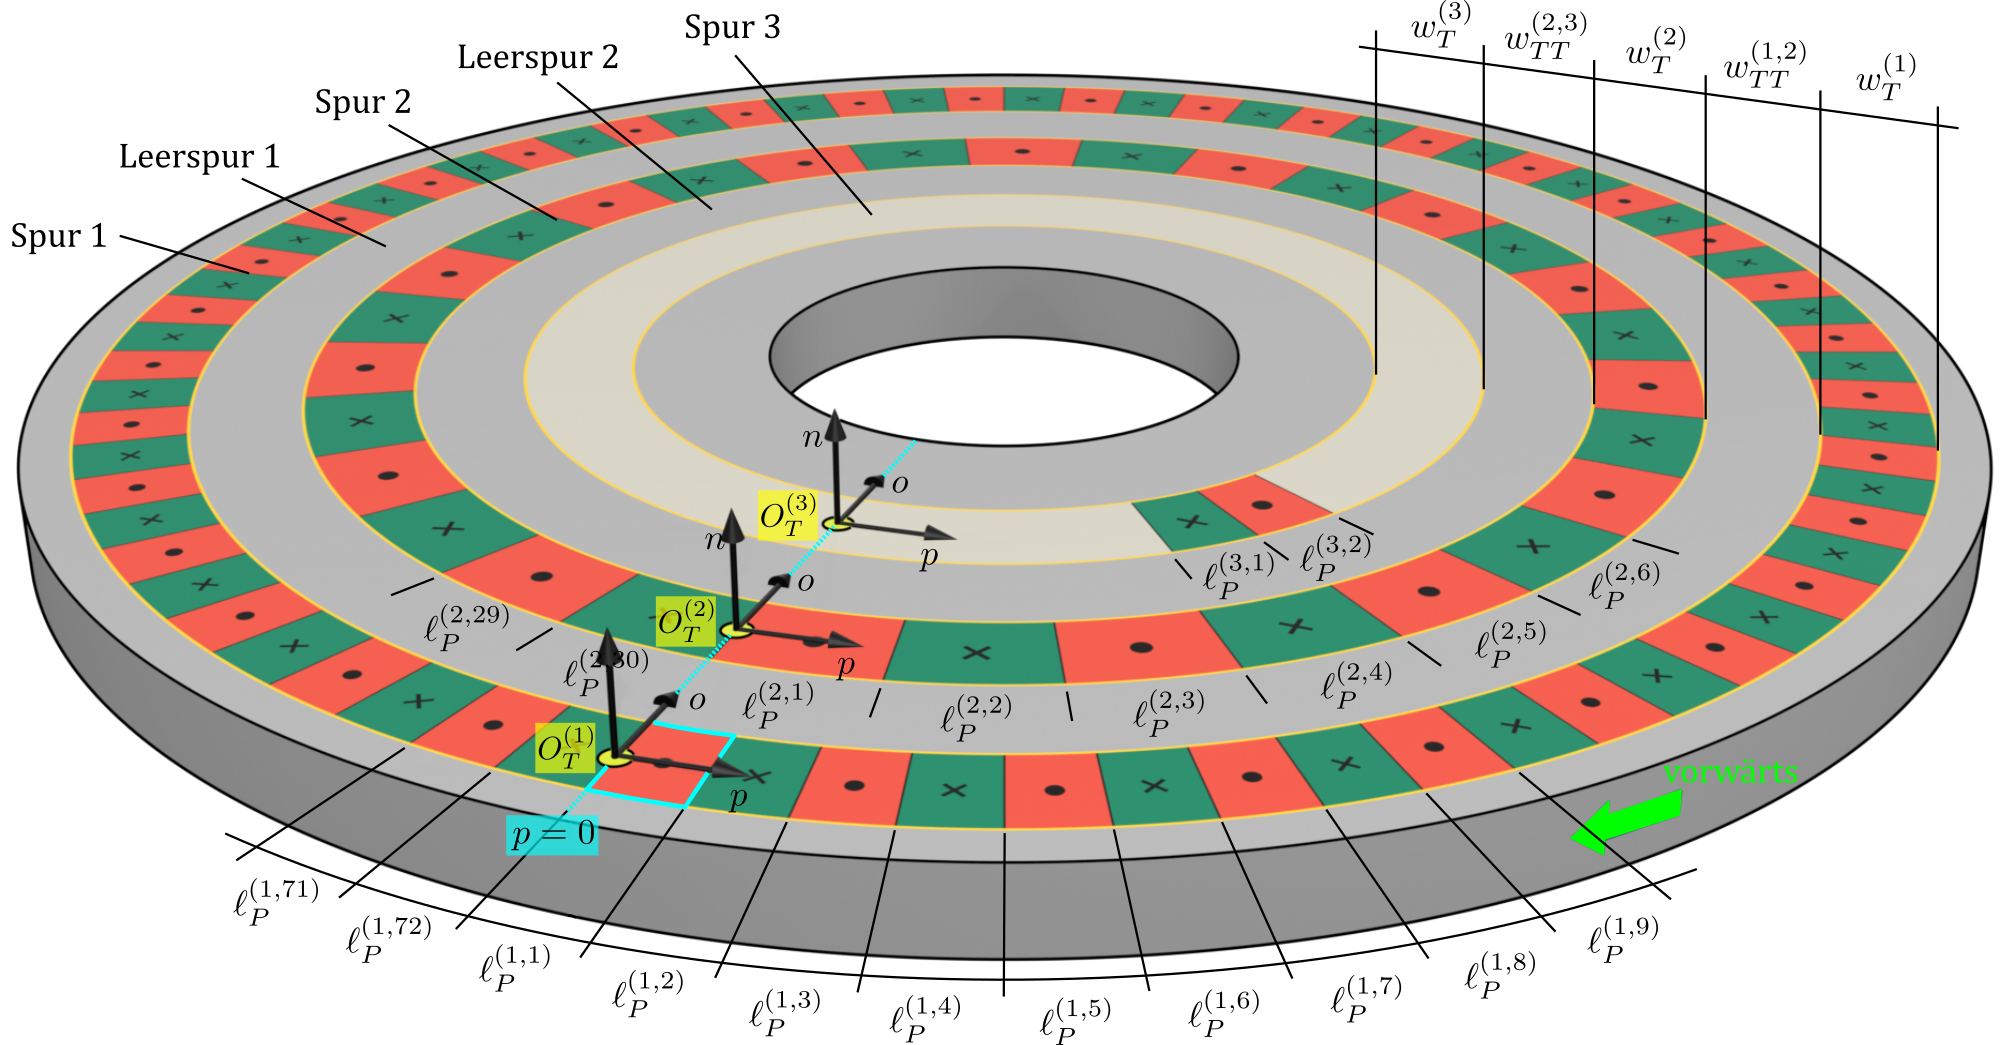
\includegraphics[width=1\linewidth,height=\textheight,keepaspectratio]{figures/sec04/20-struktur_spuren2.png}

}

\caption{\label{fig-sec04-20-struktur_spuren2}Strukturbeschreibung eines
Rotationsmaßstabs mit mehreren Spuren}

\end{figure}%

Abbildung~\ref{fig-sec04-20-struktur_spuren2} zeigt einen magnetischen
Rotationsmaßstab mit drei axialen Spuren in Poldarstellung. Spur 1 ist
als inkrementelle Spur mit \(N_P^{(1)} = 72\) Polen ausgeführt, Spur 2
als inkrementelle Spur mit \(N_P^{(2)} = 30\) Polen. Spur 3 dient als
Referenzspur und enthält ein einzelnes Referenz-Polpaar.

Die Vorwärtsbewegung ist in der Abbildung grün eingezeichnet, woraus
sich mit der funktionalen Oberfläche die \(p\)- und \(o\)-Richtungen
ergeben. Die Ordnungsindizes der Spuren sind entsprechend aufsteigend in
positiver \(o\)-Richtung von außen nach innen vergeben.

Der Beginn des ersten Pols der Spur 1 ist blau hervorgehoben und dient
hier als gemeinsamer Strukturbezug für die \(p\)-Lage der drei Spur-KS.
Die dort festgelegte Lage \(p = 0\) wird in \(o\)-Richtung auf die
übrigen Spuren übertragen und ist durch eine gepunktete blaue Linie
gekennzeichnet. Bei Spur 2 fällt der Ursprung ebenfalls mit dem Beginn
des ersten Pols zusammen, während er bei Spur 3 in einem Bereich
außerhalb des Referenz-Polpaares liegt. In \(o\)-Richtung liegen die
Ursprünge jeweils mittig auf der zugehörigen Spur. Die Ursprünge und
lokalen Koordinatenrichtungen der Spur-KS sind entsprechend
eingezeichnet.

Die Ordnungsindizes der Pole steigen in positiver \(p\)-Richtung an.
Exemplarisch dargestellte Pollängen tragen sowohl den Ordnungsindex der
Spur als auch den des jeweiligen Pols und veranschaulichen damit die
Verwendung mehrerer Ordnungsindizes für spurbezogene Polgrößen.

\begingroup
\footnotesize
\renewcommand{\baselinestretch}{1.12}\selectfont
\setlength{\tabcolsep}{5pt}
\setlength{\extrarowheight}{2.5pt}
\renewcommand{\arraystretch}{1.15}
{\begin{longtable}[]{
  >{\raggedright\arraybackslash}p{(\linewidth - 4\tabcolsep) * \real{0.2500}}
  >{\centering\arraybackslash}p{(\linewidth - 4\tabcolsep) * \real{0.1500}}
  >{\raggedright\arraybackslash}p{(\linewidth - 4\tabcolsep) * \real{0.6000}}}
\caption{Begriffe Spuren}\label{tbl-begriffe_spuren}\tabularnewline
\arrayrulecolor{tableouterrule}
\toprule\noalign{}
\rowcolor{zebrabluehead}
\begin{minipage}[b]{\linewidth}\raggedright
\textbf{Begriff}
\end{minipage} & \begin{minipage}[b]{\linewidth}\centering
\textbf{Symbol}
\end{minipage} & \begin{minipage}[b]{\linewidth}\raggedright
\textbf{Beschreibung}
\end{minipage} \\
\arrayrulecolor{tableheadrule}
\specialrule{0.35pt}{0pt}{0pt}
\endhead
\arrayrulecolor{tableouterrule}
\specialrule{0.30pt}{0pt}{0pt}
\endlastfoot
\rowcolor{zebrabluelight}
\textbf{Spuranzahl} & \(N_T\) & Gesamtzahl der nummerierten Spuren \\
\arrayrulecolor{tableline}
\specialrule{0.15pt}{0pt}{0pt}
\rowcolor{zebrabluedark}
\textbf{Spurlänge} & \(\ell_T^{(i)}\) & Ausdehnung der Spur \(i\) in
\(p\)-Richtung \\
\arrayrulecolor{tableline}
\specialrule{0.15pt}{0pt}{0pt}
\rowcolor{zebrabluelight}
\textbf{Spurbreite} & \(w_T^{(i)}\) & Ausdehnung der Spur \(i\) in
\(o\)-Richtung \\
\arrayrulecolor{tableline}
\specialrule{0.15pt}{0pt}{0pt}
\rowcolor{zebrabluedark}
\textbf{Spurtiefe} & \(d_T^{(i)}\) & Ausdehnung der Spur \(i\) in
\(n\)-Richtung \\
\arrayrulecolor{tableline}
\specialrule{0.15pt}{0pt}{0pt}
\rowcolor{zebrabluelight}
\textbf{Spurlage} & \(\vec{r}_T^{(i)}\) & Position des Spur-KS-Ursprungs
\(O_T^{(i)}\) der Spur \(i\) im Maßverkörperungs-KS; Koordinaten
\(p_T^{(i)}\), \(o_T^{(i)}\) und \(n_T^{(i)}\) \\
\arrayrulecolor{tableline}
\specialrule{0.15pt}{0pt}{0pt}
\rowcolor{zebrabluedark}
\textbf{Spur-Längsversatz}, \textbf{Spur-\(p\)-Versatz} &
\(p_{TT}^{(i_1,i_2)}\) & Versatz in \(p\)-Richtung von Spur \(i_1\) zu
Spur \(i_2\) \\
\arrayrulecolor{tableline}
\specialrule{0.15pt}{0pt}{0pt}
\rowcolor{zebrabluelight}
\textbf{Spur-Querversatz}, \textbf{Spur-\(o\)-Versatz} &
\(o_{TT}^{(i_1,i_2)}\) & Versatz in \(o\)-Richtung von Spur \(i_1\) zu
Spur \(i_2\) \\
\arrayrulecolor{tableline}
\specialrule{0.15pt}{0pt}{0pt}
\rowcolor{zebrabluedark}
\textbf{Spurabstand} & \(w_{TT}^{(i,i+1)}\) & Abstand in \(o\)-Richtung
zwischen benachbarten Spuren \\
\arrayrulecolor{tableline}
\specialrule{0.15pt}{0pt}{0pt}
\end{longtable}
}
\endgroup

\bookmarksetup{startatroot}

\chapter{Streufeld der Maßverkörperung}\label{sec-05}

Das Streufeld einer Maßverkörperung ergibt sich aus ihrer Polarisation
und Geometrie. Im Folgenden werden das Streufeld und charakteristische
Feldmerkmale beschrieben, die für die magnetische Vermessung und
Bewertung von magnetischen Maßverkörperungen relevant sind.

\section{Ermittlungsbereich und
Feldverläufe}\label{sec-05-ermittlungsbereich_und_feldverluxe4ufe}

Zur Beschreibung und Charakterisierung des Streufeldes wird dieses an
räumlichen Lagen relativ zur Maßverkörperung betrachtet. Die Gesamtheit
der dabei berücksichtigten Lagen wird als \textbf{Ermittlungsbereich}
bezeichnet. Ein Ermittlungsbereich kann sich unmittelbar aus der
Messaufgabe und der vorgesehenen Relativbewegung nach
Kapitel~\ref{sec-03} ergeben oder gezielt für die Vermessung und
Charakterisierung der Maßverkörperung festgelegt werden. Seine Lage und
Orientierung werden im Maßverkörperungs-KS oder in einem zugeordneten
Struktur-KS angegeben.

Ein eindimensionaler Ermittlungsbereich wird als \textbf{Messpfad}
bezeichnet. Verläuft ein Messpfad entlang einer einzelnen
Koordinatenrichtung, wird entsprechend von einem \textbf{\(p\)-Pfad},
\textbf{\(o\)-Pfad} oder \textbf{\(n\)-Pfad} gesprochen. Ein \(p\)-Pfad
folgt damit der \(p\)-Richtung und kann bei zylindrischen Anordnungen
gekrümmt verlaufen.

Beispielsweise beschreibt die Parametrisierung
\((p,o,n) = (t, 0{,}1\,\mathrm{mm})\) mit
\(t \in [0\,\mathrm{mm}, 5\,\mathrm{mm}]\) einen geradlinigen,
\(5\,\mathrm{mm}\) langen \(p\)-Pfad bei einer Messhöhe von
\(1\,\mathrm{mm}\). Ein entsprechender Messpfad ist in
Abbildung~\ref{fig-sec05-00-ermittlungsbereiche} (a) dargestellt.

Ein zweidimensionaler Ermittlungsbereich wird als \textbf{Messfläche},
ein dreidimensionaler Ermittlungsbereich als \textbf{Messvolumen}
bezeichnet. Analog zu Messpfaden können Messflächen anhand der
variierten Koordinatenrichtungen bezeichnet werden. Eine
\(p\)-\(o\)-Messfläche wird beispielsweise durch Variation von \(p\) und
\(o\) bei konstantem \(n\) gebildet.

Die Parametrisierung \((p,o,n) = (t,u,1\,\mathrm{mm})\) mit
\(t \in [0^\circ, 360^\circ]\) und
\(u \in [-1\,\mathrm{mm}, 1\,\mathrm{mm}]\) beschreibt beispielsweise
eine \(2\,\mathrm{mm}\) breite \(p\)-\(o\)-Messfläche bei einer Messhöhe
von \(1\,\mathrm{mm}\). Diese Messfläche ist in
Abbildung~\ref{fig-sec05-00-ermittlungsbereiche} (e) in einer radialen
Anordnung und in Teilbild (f) in einer axialen Anordnung dargestellt.

\begin{figure}[h]

\centering{

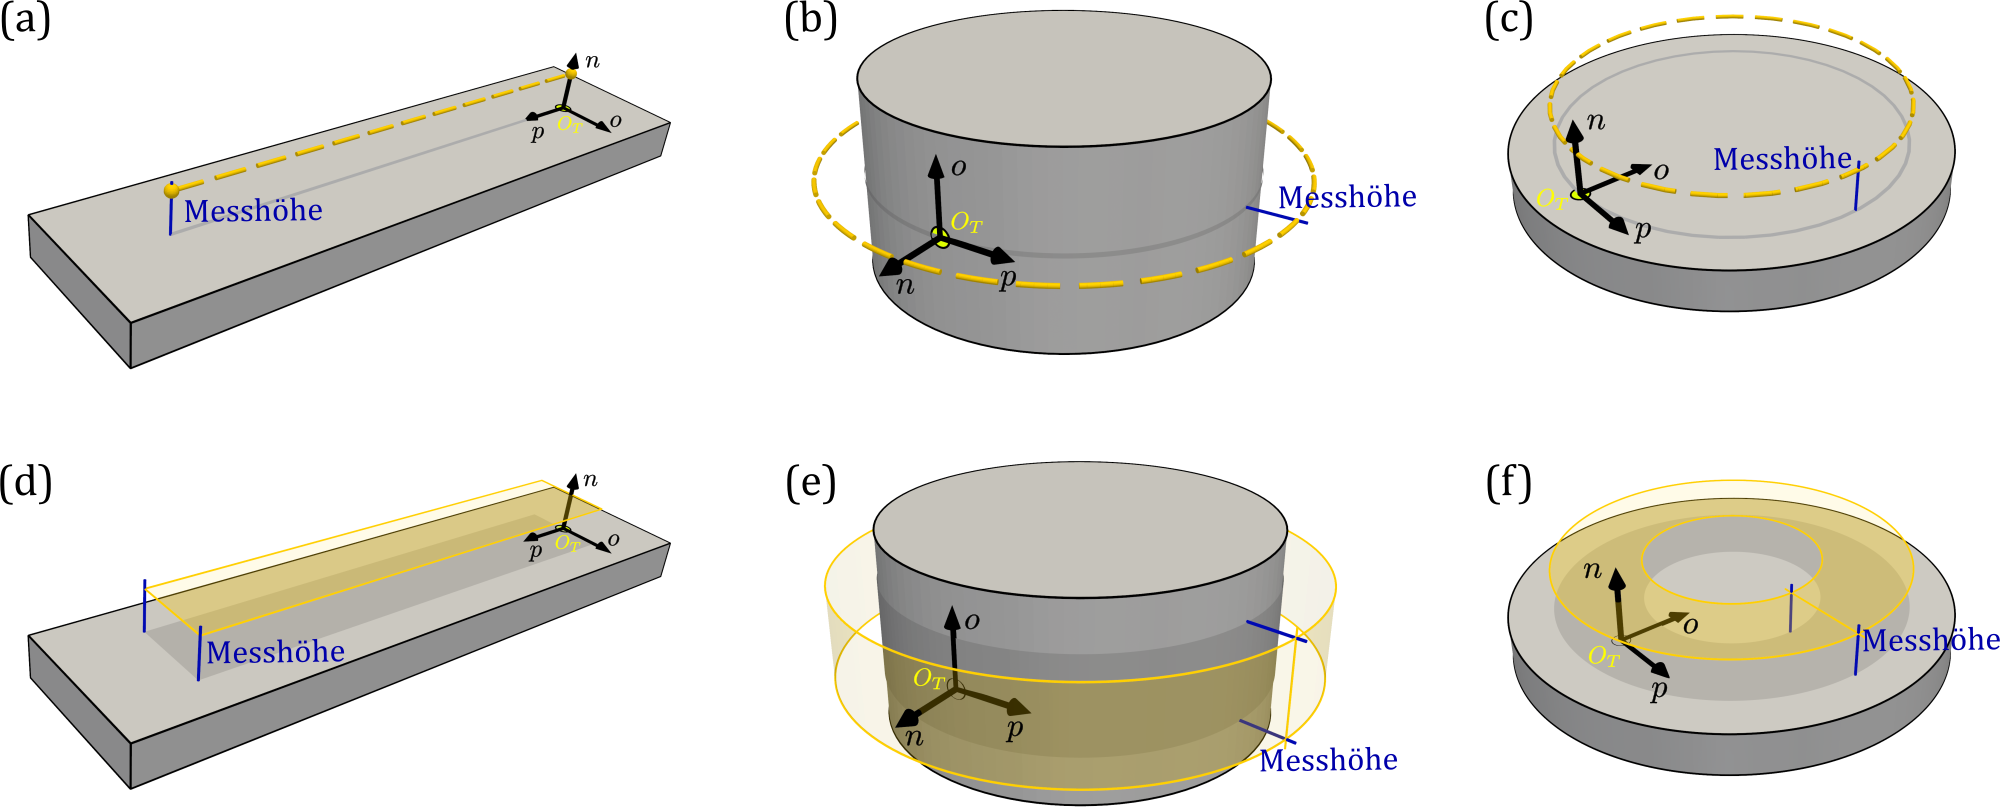
\includegraphics[width=1\linewidth,height=\textheight,keepaspectratio]{figures/sec05/00-ermittlungsbereiche.png}

}

\caption{\label{fig-sec05-00-ermittlungsbereiche}Ermittlungsbereiche}

\end{figure}%

Abbildung~\ref{fig-sec05-00-ermittlungsbereiche} zeigt beispielhafte
Ermittlungsbereiche für lineare, radiale und axiale Anordnungen. In den
Teilbildern (a) bis (c) sind \(p\)-Pfade bei konstanten \(o\) und \(n\),
in den Teilbildern (d) bis (f) \(p\)-\(o\)-Messflächen bei konstanten
Messhöhen \(n\) dargestellt.

\section{Streufeld einer
Maßverkörperung}\label{sec-05-streufeld_einer_mauxdfverkuxf6rperung}

Wie in Kapitel~\ref{sec-04-magnetpole} erläutert, lässt sich die
Streufeldcharakteristik einer magnetischen Maßverkörperung qualitativ
durch den Austritt der magnetischen Feldlinien an den Nordpolen und
ihren Eintritt an den Südpolen beschreiben. Die einzelnen Komponenten
\(B_p\) und \(B_n\) weisen dabei in \(p\)-Richtung typischerweise einen
wellenförmigen Verlauf mit Maxima, Minima und Nullstellen auf. Mit
zunehmendem Abstand von der magnetischen Struktur nimmt die Amplitude
des Streufeldes ab. Dieser Abfall erfolgt im Fernfeld einzelner Zonen
näherungsweise kubisch und bei der Überlagerung der Streufelder mehrerer
alternierender Zonen näherungsweise exponentiell (Ausserlechner 2012).

\begin{figure}[h]

\centering{

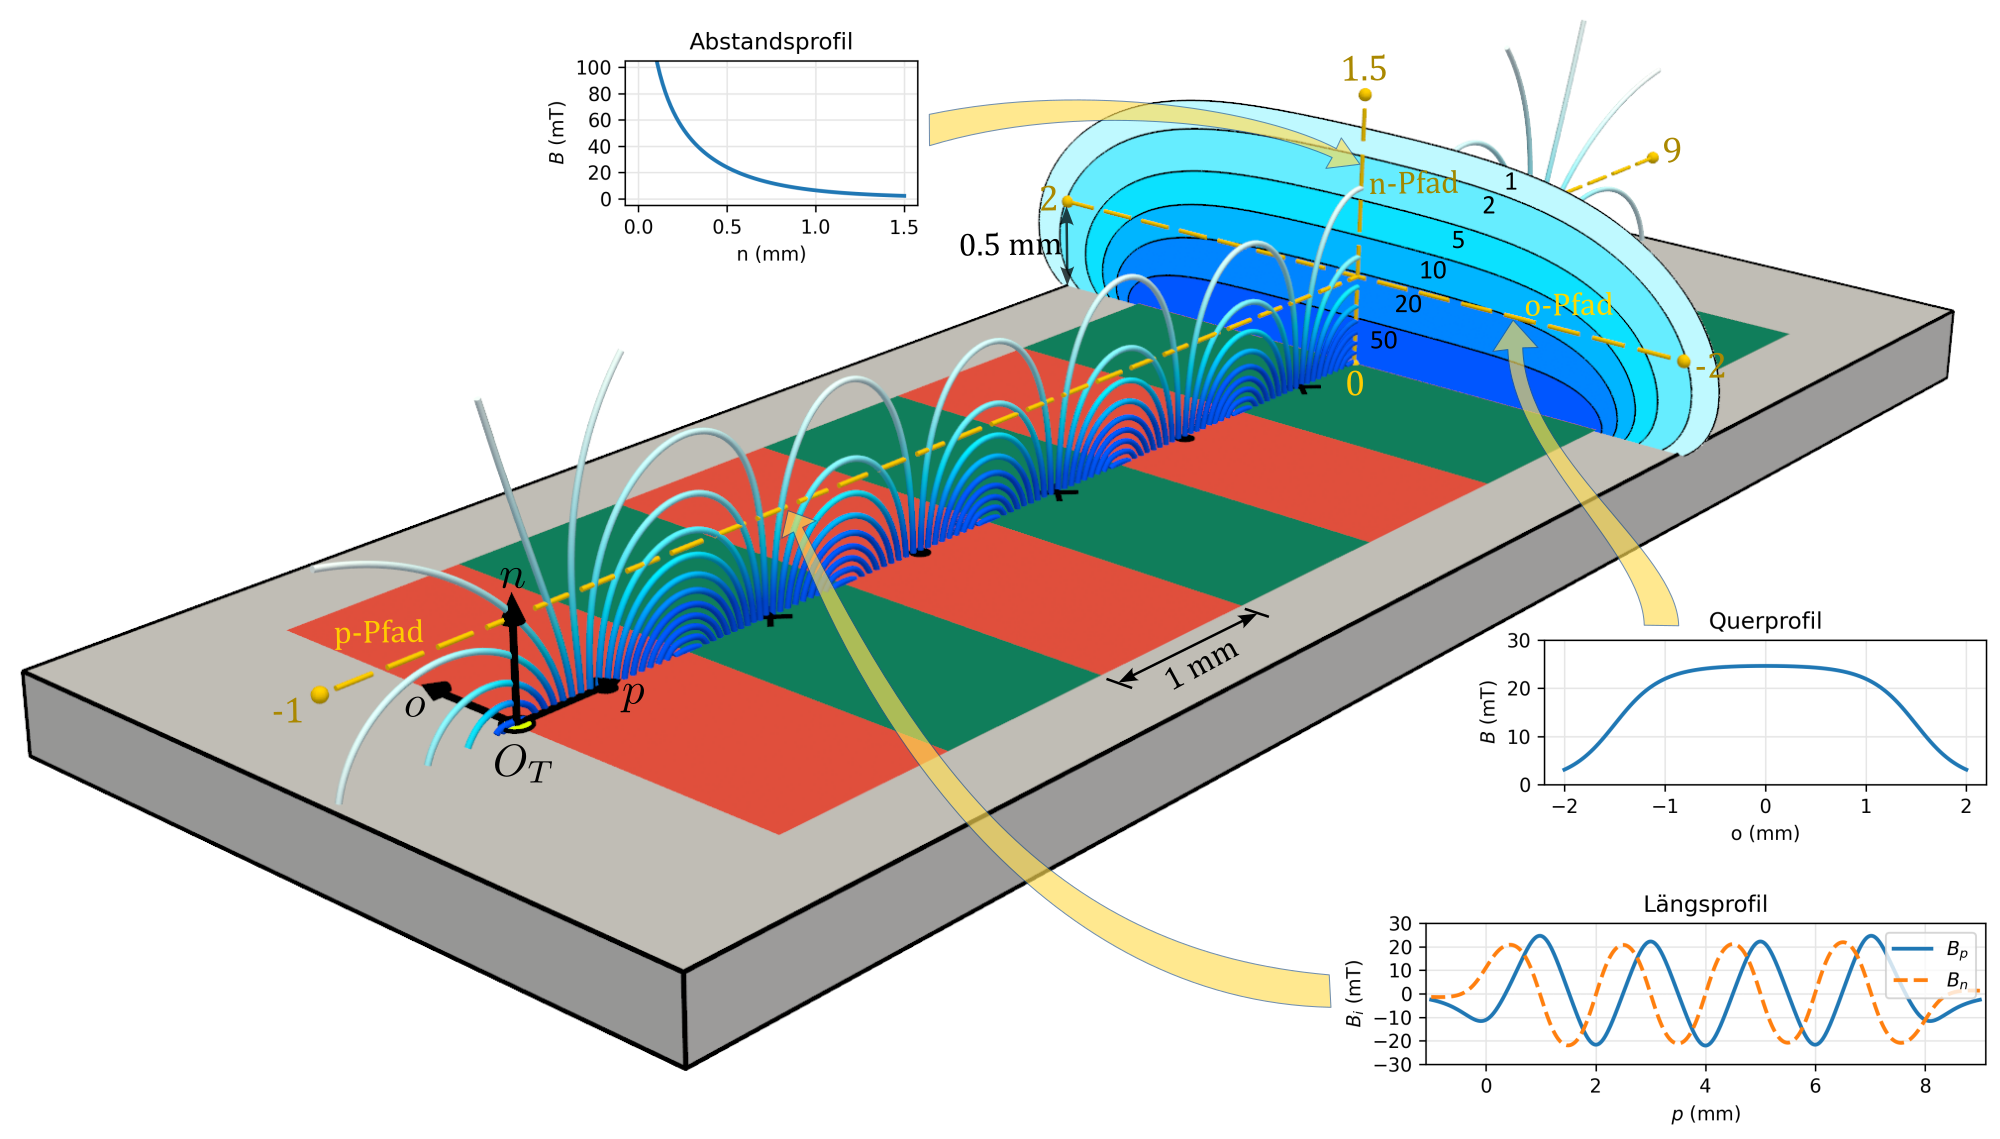
\includegraphics[width=1\linewidth,height=\textheight,keepaspectratio]{figures/sec05/01-streufeldcharakteristik.png}

}

\caption{\label{fig-sec05-01-streufeldcharakteristik}Ermittlungsbereiche}

\end{figure}%

Abbildung~\ref{fig-sec05-01-streufeldcharakteristik} zeigt das
\textbf{Simulationsergebnis} eines Multipolmagneten aus acht homogenen,
alternierend OOP-polarisierten Zonen mit Polarisationsamplituden
\(J_Z = 300\,\mathrm{mT}\), Längen \(\ell_Z = 1\,\mathrm{mm}\), Breiten
\(w_Z = 3\,\mathrm{mm}\) und Tiefen \(d_Z = 200\,\mu\mathrm{m}\). Die
Maßverkörperung ist in Poldarstellung gezeigt. Das resultierende
Streufeld ist in Form von Feldlinien mittig über der Maßverkörperung
sowie einer blauen Konturdarstellung der Streufeldamplitude in einer
\(o\)-\(n\)-Ebene dargestellt. In beiden Darstellungen codiert die blaue
Farbskala den Wert der Streufeldamplitude in Millitesla. Zur
Veranschaulichung der Streufeldcharakteristik sind zusätzlich
Feldverläufe entlang der eingezeichneten Messpfade in den Teilbildern
abgebildet.

\textbf{In \(p\)-Richtung} spiegelt das Streufeld die periodische
Struktur des Polmusters wider. Die charakteristische Oszillation der
Komponenten \(B_p\) und \(B_n\) des Streufeldes entlang des
eingezeichneten \(p\)-Pfades ist im Längsprofil erkennbar. Die
Komponenten sind gegeneinander typischerweise um etwa \(90^\circ\)
phasenverschoben, eine Eigenschaft, die in vielen Anwendungen zur
Positionsbestimmung genutzt wird.

\textbf{In \(o\)-Richtung} ist die Streufeldcharakteristik durch einen
raschen Abfall der Feldamplitude über die seitliche Begrenzung der
magnetischen Struktur hinaus gekennzeichnet. Dies ist auch aus dem
typischen Querprofil ersichtlich, in dem die Feldamplitude entlang des
eingezeichneten \(o\)-Pfades abgebildet ist. Das Querprofil
verdeutlicht, dass sich das Streufeld bei komplexen Anordnungen in der
Regel auf einen begrenzten Bereich oberhalb der magnetischen Struktur
konzentriert.

\textbf{In \(n\)-Richtung} ist die starke Abschwächung der Feldamplitude
mit wachsendem Abstand von der magnetischen Struktur sowohl an der
Konturdarstellung als auch am Abstandsprofil ersichtlich. Der rasche
Zerfall der Feldamplitude begrenzt den nutzbaren Messabstand und
erfordert eine präzise Positionierung der Sensorik nahe der funktionalen
Oberfläche der Maßverkörperung, was mit erheblichen technischen
Herausforderungen verbunden sein kann.

In \(o\)- und \(n\)-Richtung ist die Streufeldcharakteristik
insbesondere durch die Abnahme der Feldamplitude mit zunehmendem Abstand
von der magnetischen Struktur geprägt. Für die Anwendung ist dabei
entscheidend, dass die \textbf{Feldamplitude} innerhalb eines
festgelegten Wertebereichs liegt, da unterschiedliche Sensortechnologien
und Sensorausführungen nur innerhalb bestimmter Feldamplitudenbereiche
spezifizierte Messeigenschaften aufweisen.

Ein unterer \textbf{Amplitudengrenzwert} kann sich beispielsweise aus
dem erforderlichen Signal-Rausch-Verhältnis eines Sensors ergeben,
während ein oberer Amplitudengrenzwert durch den zulässigen Mess- oder
Linearitätsbereich bestimmt sein kann. Ein \textbf{Nutzbereich} wird
durch eine oder mehrere für die Anwendung festgelegte
Amplitudenbedingungen definiert.

\section{Feldmerkmale auf
Messpfaden}\label{sec-05-feldmerkmale_auf_messpfaden}

Zur Beschreibung des Streufeldes wird in der Praxis auf bestimmte
Merkmale von Feldverläufen Bezug genommen. Im Folgenden werden hierzu
zunächst eindimensionale Feldverläufe entlang ausgewählter Messpfade
betrachtet.

\textbf{Entlang eines \(p\)-Pfades} stellen insbesondere die lokalen
Maxima und Minima einer betrachteten Feldkomponente \(B_\alpha\),
insbesondere \(B_p\) und \(B_n\), die im Folgenden zusammenfassend als
\textbf{Peaks} (Bezugsindex „A``) bezeichnet werden, sowie die
\textbf{Nullstellen} (Bezugsindex „N``) charakteristische Merkmale eines
Feldverlaufs dar. Sie werden in vielen Anwendungen für die
Positionserkennung genutzt.

Die \(p\)-Position eines Peaks wird als \textbf{Peaklage} \(p_A\), die
einer Nullstelle als \textbf{Nullstellenlage} \(p_N\) bezeichnet. Der
Wert der betrachteten Feldkomponente an einem Peak wird als
\textbf{Peakamplitude} \(B_A\) bezeichnet. Zur eindeutigen Kennzeichnung
werden Peaks und Nullstellen beginnend mit 1, entlang der positiven
\(p\)-Richtung fortlaufend nummeriert. Die Indizierung wird im
Normalfall so gewählt, dass auf die Nullstelle \(j\) der Peak \(j\)
folgt. Die \textbf{Peakanzahl} \(N_A\) und die
\textbf{Nullstellenanzahl} \(N_N\) geben die Gesamtzahl der jeweils
indizierten Merkmale an. Eine vollständige Indizierung aller Peaks und
Nullstellen ist nicht erforderlich.

Ein weiteres wichtiges Merkmal eines Feldverlaufs entlang eines
\(p\)-Pfades ist die Länge seiner Schwingungen. Die \textbf{magnetische
Halbperiode} bezeichnet den Abstand in \(p\)-Richtung zwischen zwei
benachbarten Merkmalen gleicher Art. Dabei bezeichnet \(\ell_A\) den
Abstand zwischen zwei benachbarten Peaks entgegengesetzten Vorzeichens
und \(\ell_N\) den Abstand zwischen zwei benachbarten Nullstellen:

\[
\ell_A^{(j)} = p_A^{(j+1)} - p_A^{(j)},
\]

\[
\ell_N^{(j)} = p_N^{(j+1)} - p_N^{(j)}.
\]

Die \textbf{magnetische Periode} beschreibt entsprechend die lokale
Länge einer vollständigen Schwingung. Sie wird aus dem Abstand jedes
zweiten Merkmals gleicher Art bestimmt:

\[
L_A^{(j)} = p_A^{(j+2)} - p_A^{(j)}
= \ell_A^{(j)} + \ell_A^{(j+1)},
\]

\[
L_N^{(j)} = p_N^{(j+2)} - p_N^{(j)}
= \ell_N^{(j)} + \ell_N^{(j+1)}.
\]

Da die Feldverläufe im Allgemeinen nicht streng periodisch sind, handelt
es sich bei der magnetischen Halbperiode und der magnetischen Periode um
lokale Größen, deren Werte entlang des Feldverlaufs variieren können.

\begin{figure}[h]

\centering{

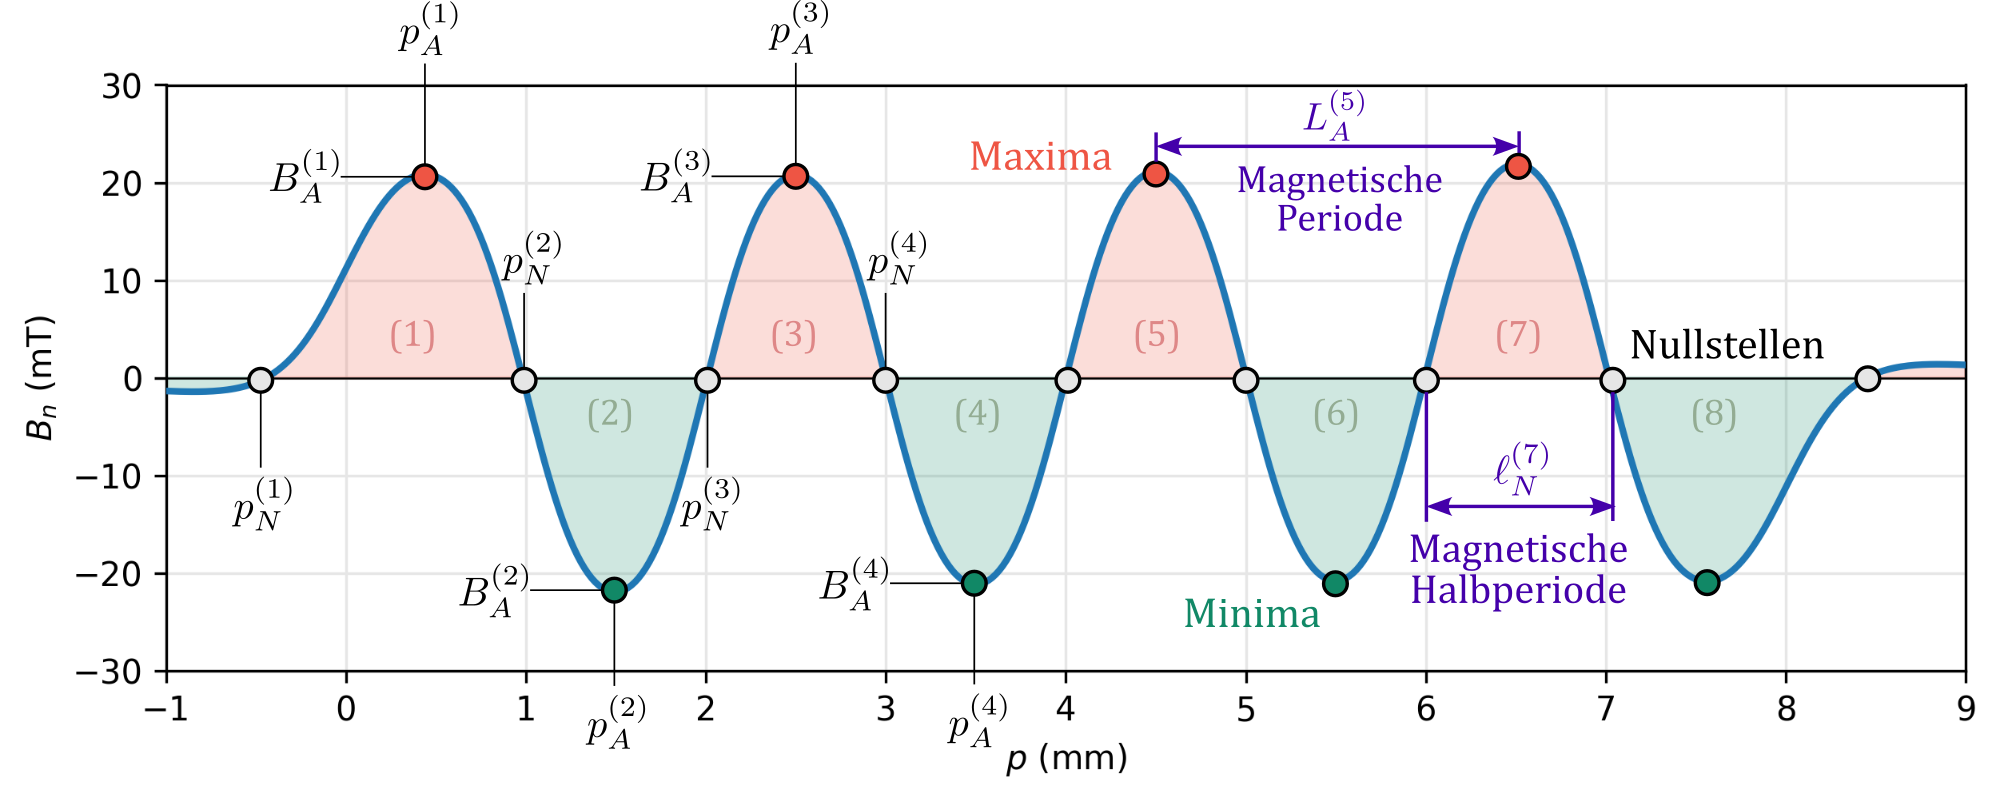
\includegraphics[width=1\linewidth,height=\textheight,keepaspectratio]{figures/sec05/02-langsprofil.png}

}

\caption{\label{fig-sec05-02-langsprofil}Feldverlauf entlang eines
\(p\)-Pfades}

\end{figure}%

Abbildung~\ref{fig-sec05-02-langsprofil} zeigt das Längsprofil
\(B_n(p)\) entlang des in
Abbildung~\ref{fig-sec05-01-streufeldcharakteristik} dargestellten
\(p\)-Pfades in detaillierter Form. Peaklagen, Nullstellenlagen,
magnetische Halbperioden und magnetische Perioden sind eingezeichnet.
Positive und negative Halbwellen sind zur Veranschaulichung rot
beziehungsweise grün hervorgehoben.

Die \textbf{Halbwelle} benennt den Abschnitt eines Feldverlaufs, der
zwischen zwei benachbarten Nullstellen liegt. Innerhalb einer Halbwelle
weist die betrachtete Feldkomponente ein einheitliches Vorzeichen auf.
Der Begriff ermöglicht eine eindeutige Bezugnahme auf einzelne
Abschnitte des Feldverlaufs und wird für deren Beschreibung und
Vermessung verwendet.

Halbwellen werden, beginnend mit 1, entlang der positiven \(p\)-Richtung
fortlaufend nummeriert. Die Halbwelle \(j\) liegt zwischen den
Nullstellen mit den Indizes \(j\) und \(j + 1\) und enthält den Peak
\(j\). Ihre Ausdehnung in \(p\)-Richtung entspricht der
nullstellenbezogenen Halbperiode \(\ell_N^{(j)}\).

\textbf{Entlang eines \(o\)-Pfades} ist insbesondere der seitliche
Verlauf der Feldamplitude von Bedeutung. Charakteristische Merkmale
eines Feldverlaufs \(B(o)\) sind die \textbf{Amplitudengrenzpunkte}. Sie
kennzeichnen die \textbf{Amplitudengrenzlagen} \(o_G\), an denen die
Feldamplitude einen vorgegebenen \textbf{Amplitudengrenzwert} \(B_G\)
annimmt, und werden, beginnend mit 1, entlang der positiven Pfadrichtung
fortlaufend nummeriert.

Die Amplitudengrenzpunkte begrenzen den Nutzbereich entlang des
betrachteten Messpfades. Die \textbf{Nutzbereichsbreite} \(w_G(p)\)
entspricht dessen Ausdehnung in \(o\)-Richtung an der Position \(p\).
Wird die Nutzbereichsbreite innerhalb einer Halbwelle \(j\) bestimmt,
wird sie als \textbf{Nutzbreite der Halbwelle} \(w_G^{(j)}(p)\)
bezeichnet.

\begin{figure}[h]

\centering{

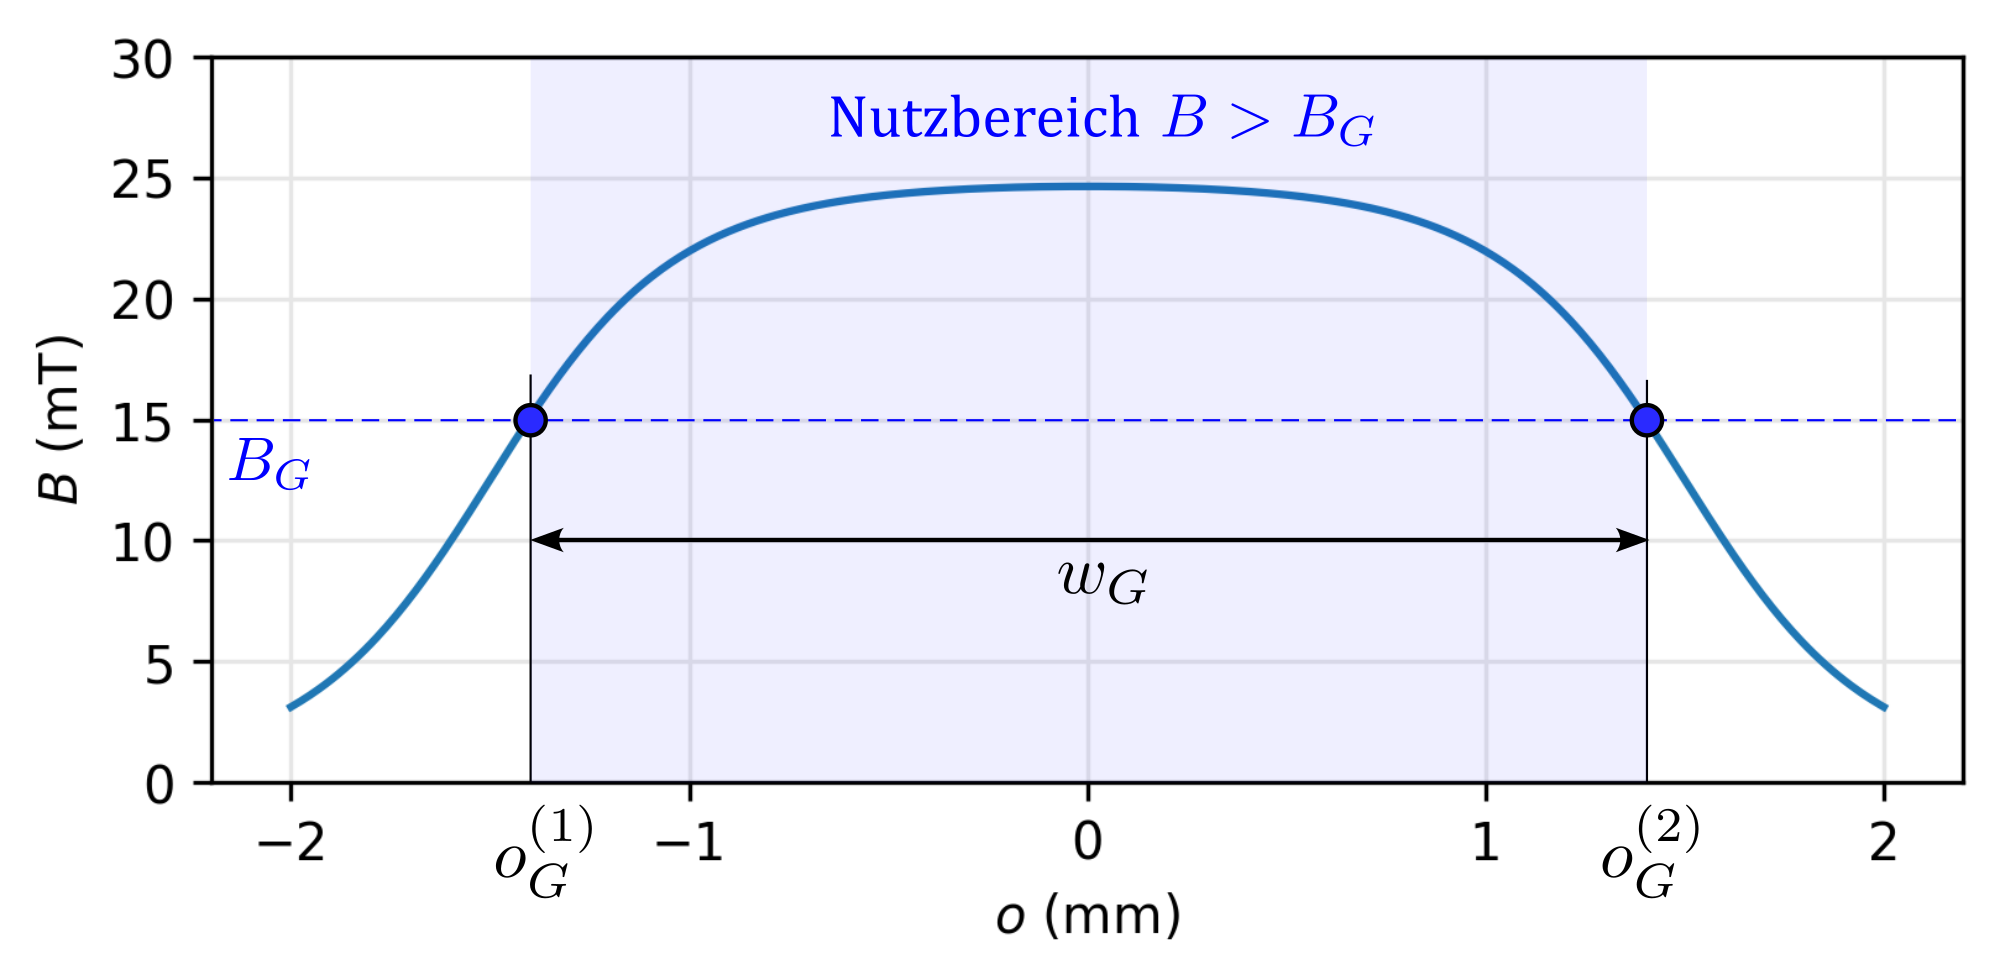
\includegraphics[width=0.7\linewidth,height=\textheight,keepaspectratio]{figures/sec05/03-querprofil.png}

}

\caption{\label{fig-sec05-03-querprofil}Feldverlauf entlang eines
\(o\)-Pfades}

\end{figure}%

Abbildung~\ref{fig-sec05-03-querprofil} zeigt das Querprofil \(B(o)\)
entlang des in Abbildung~\ref{fig-sec05-01-streufeldcharakteristik}
dargestellten \(o\)-Pfades in detaillierter Form. Ein unterer
Amplitudengrenzwert \(B_G\) definiert einen Nutzbereich. Die beiden
resultierenden Amplitudengrenzpunkte sind blau eingezeichnet. Ihre
\(o\)-Lagen entsprechen den Amplitudengrenzlagen \(o_G^{(1)}\) und
\(o_G^{(2)}\), die den Nutzbereich begrenzen.

\begin{tcolorbox}[enhanced jigsaw, arc=.35mm, bottomrule=.15mm, bottomtitle=1mm, breakable, colback=white, colbacktitle=quarto-callout-tip-color!10!white, colframe=quarto-callout-tip-color-frame, coltitle=black, left=2mm, leftrule=.75mm, opacityback=0, opacitybacktitle=0.6, rightrule=.15mm, title=\textcolor{quarto-callout-tip-color}{\faLightbulb}\hspace{0.5em}{HINWEIS}, titlerule=0mm, toprule=.15mm, toptitle=1mm]

\emph{Die in diesem Kapitel dargestellten Feldverläufe zeigen
idealisierte beziehungsweise für viele Anwendungen angestrebte Kurven
mit eindeutig ausgeprägten und gut auswertbaren Feldmerkmalen. Reale
Feldverläufe können hiervon infolge von Fertigungsabweichungen,
Materialinhomogenitäten und Randeffekten abweichen. Insbesondere bei
sehr kleinen Messhöhen, \(n \ll \ell_P\), treten höhere räumliche
Harmonische deutlicher hervor, wodurch beispielsweise zusätzliche Peaks
und Nullstellen, \textbf{Doppelpeaks} oder komplexere Feldverläufe
auftreten können.}

\end{tcolorbox}

\begingroup
\footnotesize
\renewcommand{\baselinestretch}{1.12}\selectfont
\setlength{\tabcolsep}{5pt}
\setlength{\extrarowheight}{2.5pt}
\renewcommand{\arraystretch}{1.15}
{\begin{longtable}[]{
  >{\raggedright\arraybackslash}p{(\linewidth - 4\tabcolsep) * \real{0.2500}}
  >{\centering\arraybackslash}p{(\linewidth - 4\tabcolsep) * \real{0.1500}}
  >{\raggedright\arraybackslash}p{(\linewidth - 4\tabcolsep) * \real{0.6000}}}
\caption{Begriffe Feldmerkmale}\label{tbl-begriffe-feldmerkmale}\tabularnewline
\arrayrulecolor{tableouterrule}
\toprule\noalign{}
\rowcolor{zebrabluehead}
\begin{minipage}[b]{\linewidth}\raggedright
\textbf{Begriff}
\end{minipage} & \begin{minipage}[b]{\linewidth}\centering
\textbf{Symbol}
\end{minipage} & \begin{minipage}[b]{\linewidth}\raggedright
\textbf{Beschreibung}
\end{minipage} \\
\arrayrulecolor{tableheadrule}
\specialrule{0.35pt}{0pt}{0pt}
\endhead
\arrayrulecolor{tableouterrule}
\specialrule{0.30pt}{0pt}{0pt}
\endlastfoot
\rowcolor{zebrabluelight}
\textbf{Peaklage} & \(p_A^{(j)}\) & \(p\)-Position des Peaks \(j\) \\
\arrayrulecolor{tableline}
\specialrule{0.15pt}{0pt}{0pt}
\rowcolor{zebrabluedark}
\textbf{Peakamplitude} & \(B_A^{(j)}\) & Wert der betrachteten
Feldkomponente am Peak \(j\) \\
\arrayrulecolor{tableline}
\specialrule{0.15pt}{0pt}{0pt}
\rowcolor{zebrabluelight}
\textbf{Nullstellenlage} & \(p_N^{(j)}\) & \(p\)-Position der Nullstelle
\(j\) \\
\arrayrulecolor{tableline}
\specialrule{0.15pt}{0pt}{0pt}
\rowcolor{zebrabluedark}
\textbf{Magnetische Halbperiode} & \(\ell_A^{(j)}\), \(\ell_N^{(j)}\) &
Lokale Länge einer halben Schwingung, bestimmt aus Peaks bzw.
Nullstellen mit Indizes \(j\) und \(j + 1\) \\
\arrayrulecolor{tableline}
\specialrule{0.15pt}{0pt}{0pt}
\rowcolor{zebrabluelight}
\textbf{Magnetische Periode} & \(L_A^{(j)}\), \(L_N^{(j)}\) & Lokale
Länge einer vollständigen Schwingung, bestimmt aus Peaks bzw.
Nullstellen mit Indizes \(j\) und \(j + 2\) \\
\arrayrulecolor{tableline}
\specialrule{0.15pt}{0pt}{0pt}
\rowcolor{zebrabluedark}
\textbf{Amplitudengrenzwert} & \(B_G\) & Für die Anwendung festgelegter
Grenzwert der Feldamplitude \\
\arrayrulecolor{tableline}
\specialrule{0.15pt}{0pt}{0pt}
\rowcolor{zebrabluelight}
\textbf{Amplitudengrenzlage} & \(o_G^{(j)}\) & \(o\)-Lage des
Amplitudengrenzpunkts \(j\) \\
\arrayrulecolor{tableline}
\specialrule{0.15pt}{0pt}{0pt}
\rowcolor{zebrabluedark}
\textbf{Nutzbereichsbreite} & \(w_G(p)\) & Ausdehnung des Nutzbereichs
in \(o\)-Richtung an der Position \(p\) \\
\arrayrulecolor{tableline}
\specialrule{0.15pt}{0pt}{0pt}
\rowcolor{zebrabluelight}
\textbf{Nutzbreite der Halbwelle} & \(w_G^{(j)}(p)\) &
Nutzbereichsbreite innerhalb der Halbwelle \(j\) \\
\arrayrulecolor{tableline}
\specialrule{0.15pt}{0pt}{0pt}
\end{longtable}
}
\endgroup

\section{Feldmerkmale auf Messflächen und im
Raum}\label{sec-05-feldmerkmale_flaechen_raum}

\textbf{Messflächen} geben einen zweidimensionalen Einblick in die
Streufeldcharakteristik. Besonders zweckmäßig ist dafür die Darstellung
einer anwendungsrelevanten Streufeldkomponente auf einer
\(p\)-\(o\)-Messfläche bei konstanter Messhöhe \(n\). Amplitudengrenzen,
die den Nutzbereich eingrenzen, erscheinen auf einer solchen Messfläche
als Konturlinien der Feldamplitude und werden dem Feldverlauf häufig
ergänzend überlagert.

\begin{figure}[h]

\centering{

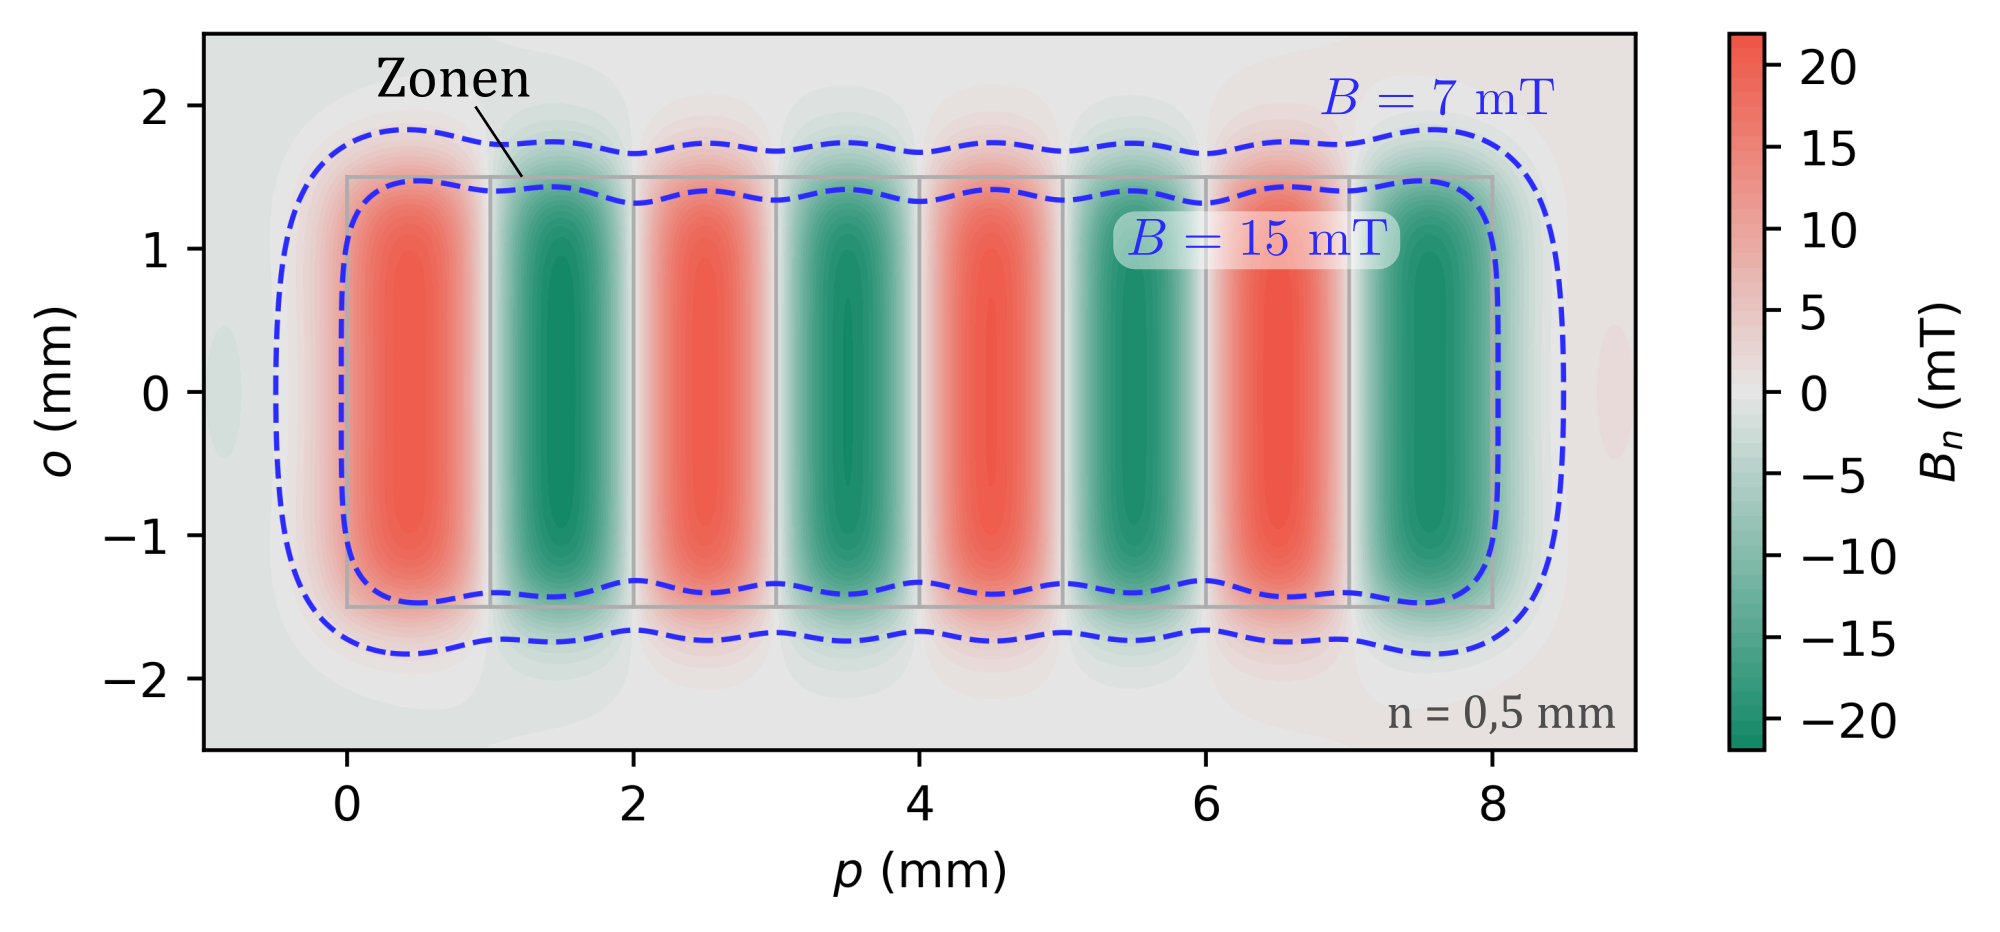
\includegraphics[width=0.75\linewidth,height=\textheight,keepaspectratio]{figures/sec05/04-feldverlauf_2D.png}

}

\caption{\label{fig-sec05-04-feldverlauf_2D}Feldverlauf auf
\(p\)-\(o\)-Messfläche}

\end{figure}%

Abbildung~\ref{fig-sec05-04-feldverlauf_2D} zeigt den Feldverlauf
\(B_n(p,o)\) der in Kapitel~\ref{sec-05-streufeld_einer_maßverkörperung}
beschriebenen Maßverkörperung bei der Messhöhe
\(n = 0{,}5\,\mathrm{mm}\). Die Projektion der darunterliegenden Zonen,
die das Streufeld erzeugen, ist grau umrandet. Zusätzlich sind die
Konturlinien der Feldamplitude für die Amplitudengrenzwerte
\(B_G = 7\,\mathrm{mT}\) und \(B_G = 15\,\mathrm{mT}\) eingezeichnet.
Sie veranschaulichen die Abgrenzung möglicher Nutzbereiche auf der
Messfläche. Die Farbwahl bei der Darstellung des Feldverlaufs folgt der
in Kapitel~\ref{sec-04-darstellungskonventionen} festgelegten
Darstellungskonvention.

Abbildung~\ref{fig-sec05-04-feldverlauf_2D} veranschaulicht zwei
\textbf{grundlegende Eigenschaften} des Feldverlaufs. In \(p\)-Richtung
oszilliert die dargestellte Feldkomponente, wobei positive Halbwellen
rot und negative Halbwellen grün dargestellt sind. Über die seitliche
Begrenzung der magnetischen Struktur hinaus nimmt die Amplitude des
Feldes rasch ab.

Für Kommunikationszwecke wird der zweidimensionale Feldverlauf häufig
auf ein binäres Farbmuster reduziert, was eine kompakte und anschauliche
Darstellung der wesentlichen Feldmerkmale ermöglicht. Bei den
Amplitudengrenzen handelt es sich um zweidimensionale Fortsetzungen der
auf Messpfaden auftretenden Grenzpunkte. Gleichermaßen setzen sich die
Nullstellen auf der Messfläche zu \textbf{Nulllinien} fort. Sie bilden
die Grenzen benachbarter Halbwellen. Peaklagen setzen sich zu
\textbf{Peaklinien} fort, bei denen es sich mathematisch um
Extremwertlinien in \(p\)-Richtung handelt.

\begin{figure}[h]

\centering{

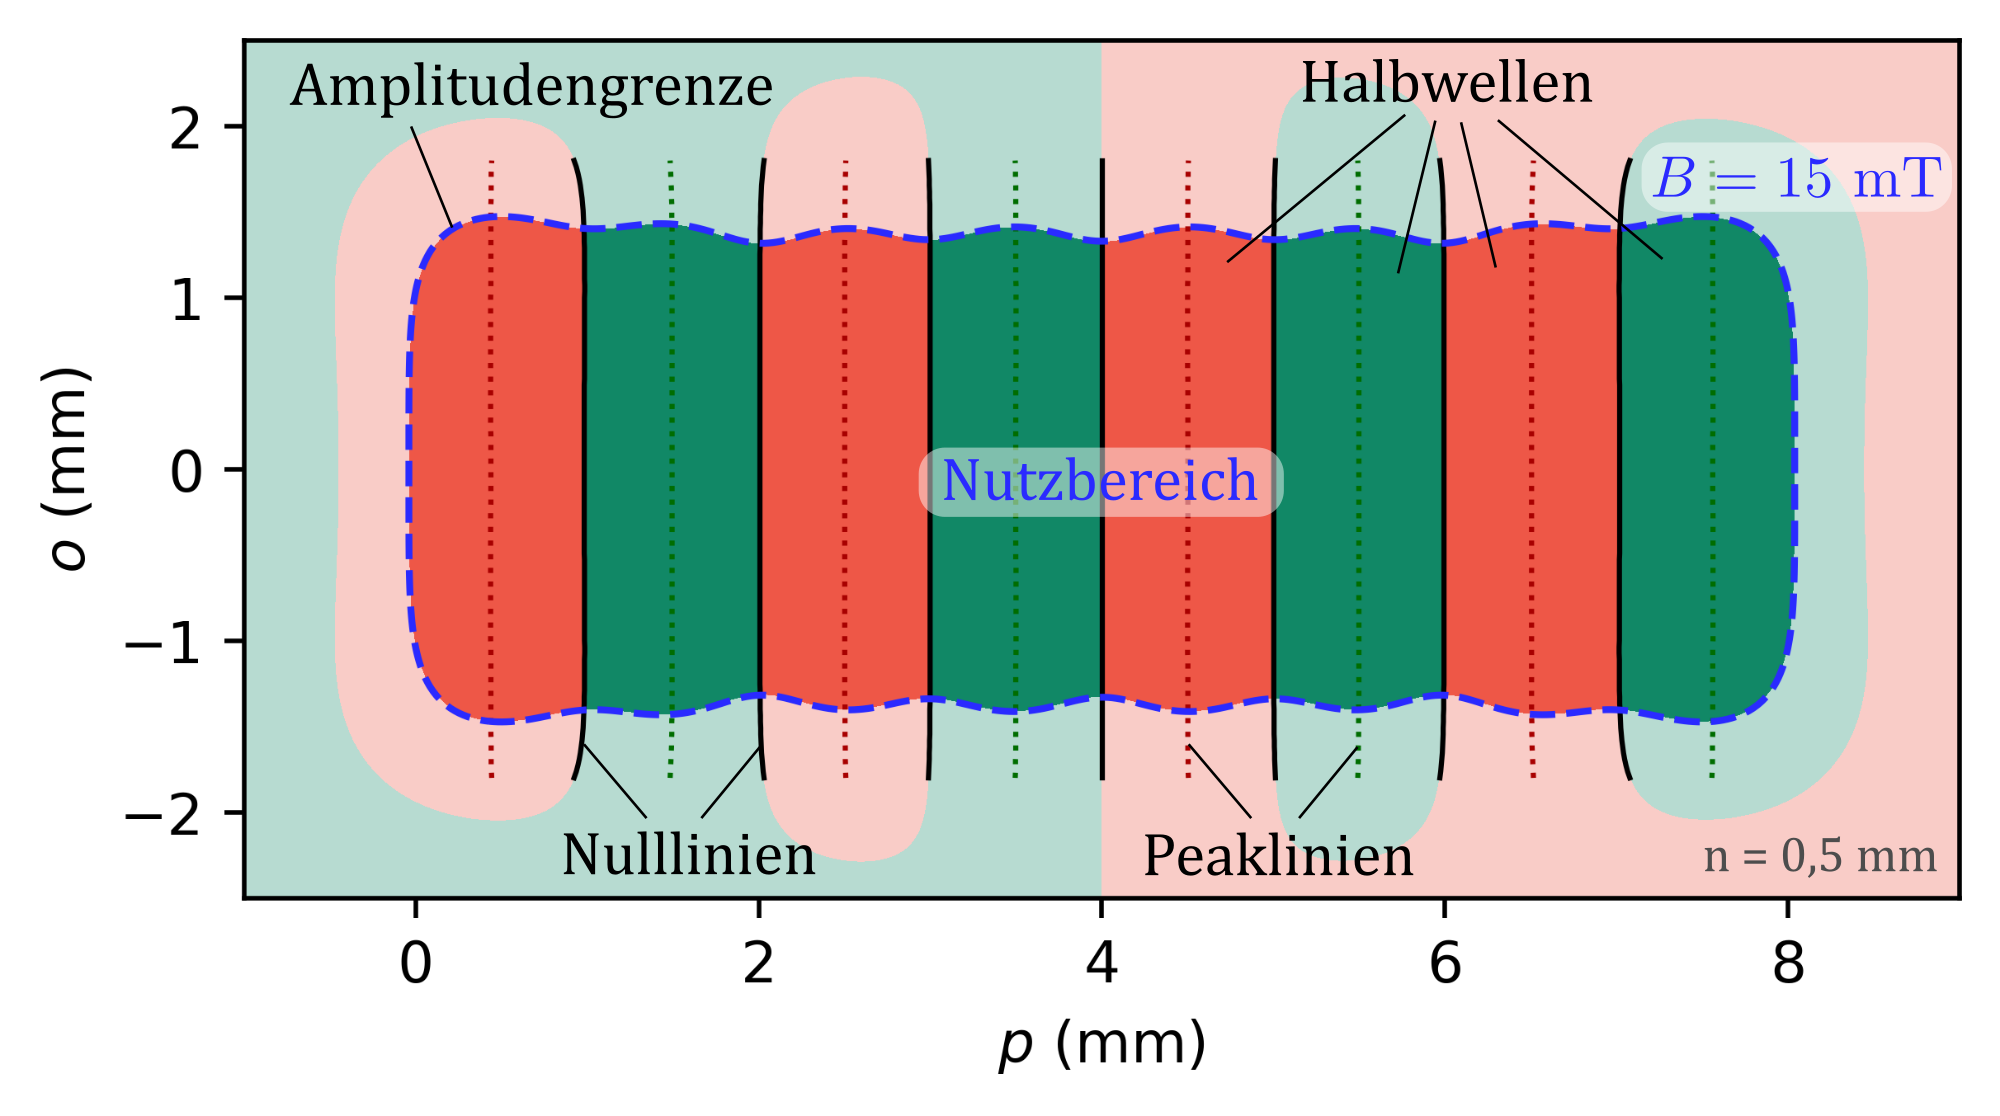
\includegraphics[width=0.75\linewidth,height=\textheight,keepaspectratio]{figures/sec05/05-feldverlauf_2D_binar.png}

}

\caption{\label{fig-sec05-05-feldverlauf_2D_binar}Feldverlauf auf
\(p\)-\(o\)-Messfläche in binärer Form}

\end{figure}%

Abbildung~\ref{fig-sec05-05-feldverlauf_2D_binar} zeigt den Feldverlauf
\(B_n(p,o)\) aus Abbildung~\ref{fig-sec05-04-feldverlauf_2D} in binärer
Farbdarstellung. Dem Farbmuster sind die Feldmerkmale in Form von
Nulllinien und Peaklinien sowie die Amplitudengrenzlinie für
\(B_G = 15\,\mathrm{mT}\) überlagert. Der durch diesen
Amplitudengrenzwert festgelegte Nutzbereich ist farblich hervorgehoben.
Die Nulllinien gliedern ihn sichtbar in positive und negative
Halbwellen.

Innerhalb des Nutzbereichs weisen die Komponenten \(B_p\) und \(B_n\)
typischerweise eine geordnete, \textbf{wellenförmige Struktur} auf, die
eine eindeutige Abgrenzung und Zuordnung der Halbwellen ermöglicht.
Außerhalb des Nutzbereichs ist diese geordnete Struktur nicht
notwendigerweise erhalten, wie auch in der Abbildung erkennbar.
Nulllinien können dort zusammenlaufen oder sich so verändern, dass
einzelne Halbwellen nicht mehr eindeutig abgegrenzt und fortlaufend
zugeordnet werden können. Für die anwendungsbezogene Referenzierung nach
Kapitel~\ref{sec-05-feldmerkmale_auf_messpfaden} werden auf Messflächen
daher vorrangig die innerhalb des Nutzbereichs liegenden Halbwellen
betrachtet.

Feldverläufe auf Messpfaden und Messflächen zeigen jeweils nur
Ausschnitte des \textbf{räumlichen Streufeldes} einer Maßverkörperung.
Seine Struktur in ihrer Gesamtheit zu verstehen, ist für die Auslegung
magnetischer Messsysteme von wesentlicher Bedeutung.

Die räumlichen Fortsetzungen der Nullstellen werden als
\textbf{Nullstellenflächen} bezeichnet. Mathematisch handelt es sich um
Isoflächen einer betrachteten Feldkomponente zum Feldwert null. Sie
werden durch folgende Gleichung beschrieben:

\[
B_\alpha(p,o,n) = 0.
\]

Die räumlichen Fortsetzungen der Peaklagen werden als
\textbf{Peakflächen} bezeichnet. Dabei handelt es sich um
Extremwertflächen der betrachteten Feldkomponente in \(p\)-Richtung, für
die notwendigerweise gilt:

\[
\frac{\partial}{\partial p} B_\alpha(p,o,n) = 0.
\]

Amplitudengrenzen sind räumlich durch \textbf{Amplitudengrenzflächen}
definiert. Sie sind Isoflächen der Streufeldamplitude zu einem
festgelegten Amplitudengrenzwert \(B_G\):

\[
B(p,o,n) = B_G.
\]

Wenn Messpfade und Messflächen diese räumlichen Flächen schneiden,
entstehen \textbf{Schnittpunkte} beziehungsweise \textbf{Schnittlinien}.
Der Schnitt einer Nullstellenfläche mit einem Messpfad ergibt eine
Nullstelle, der Schnitt mit einer Messfläche eine Nulllinie.
Entsprechend ergeben sich aus dem Schnitt mit Peakflächen Peaklagen
beziehungsweise Peaklinien und aus den Schnitten mit
Amplitudengrenzflächen Amplitudengrenzpunkte beziehungsweise
Amplitudengrenzlinien.

Im dreidimensionalen Raum wird der \textbf{Nutzbereich} durch
Amplitudengrenzflächen begrenzt und durch Nullstellenflächen in
Halbwellen unterteilt.

\begin{figure}[h]

\centering{

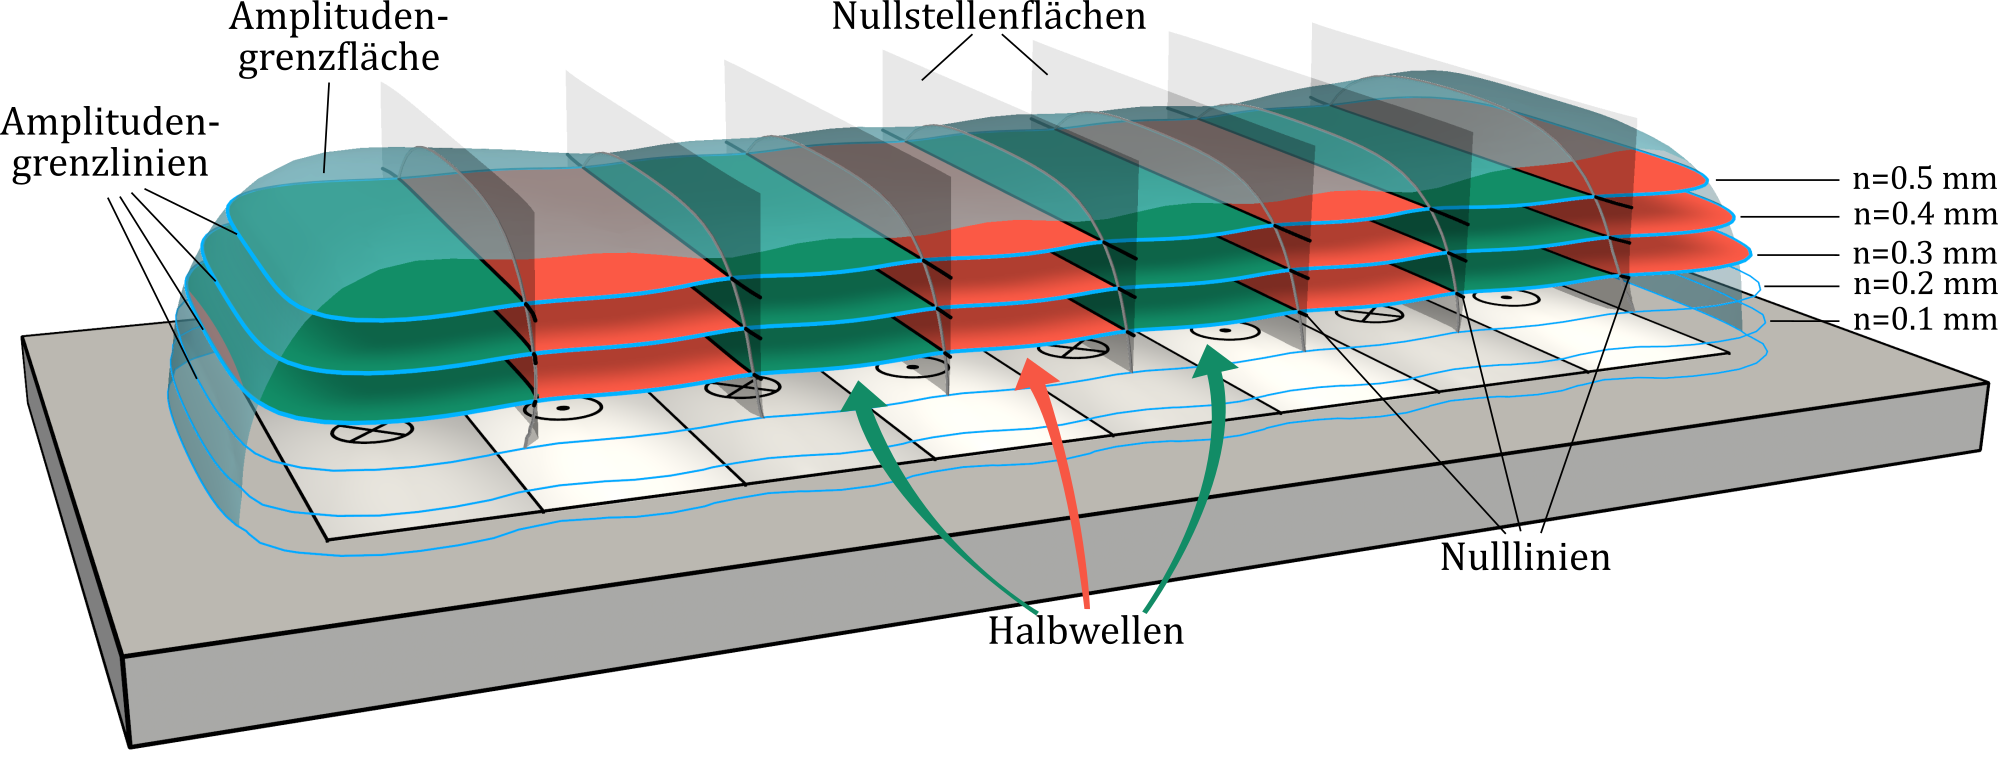
\includegraphics[width=1\linewidth,height=\textheight,keepaspectratio]{figures/sec05/06-feldverlauf_3D.png}

}

\caption{\label{fig-sec05-06-feldverlauf_3D}Feldverlauf im Raum}

\end{figure}%

Abbildung~\ref{fig-sec05-06-feldverlauf_3D} veranschaulicht die
räumliche Anordnung ausgewählter Merkmale der OOP-Komponente des
Streufeldes über der in
Kapitel~\ref{sec-05-streufeld_einer_maßverkörperung} beschriebenen
Maßverkörperung. Die Amplitudengrenzfläche des durch
\(B_G = 15\,\mathrm{mT}\) festgelegten Nutzbereichs ist blau
dargestellt. Sie bildet eine blasenförmige Hüllfläche über der
Maßverkörperung, die in der Abbildung zur besseren Sichtbarkeit nach
vorne hin aufgeschnitten dargestellt ist. In der Abbildung ist die
\(n\)-Koordinate um einen Faktor 2 gestreckt, damit die Feldverteilung
besser erkennbar ist.

Innerhalb des Nutzbereichs ist die Feldkomponente \(B_n\) auf den
\(p\)-\(o\)-Messflächen bei \(n = 0{,}4\,\mathrm{mm}\),
\(n = 0{,}5\,\mathrm{mm}\) und \(n = 0{,}6\,\mathrm{mm}\) in binärer
Farbdarstellung gezeigt. Die Schnittlinien dieser Messflächen mit der
Amplitudengrenzfläche bilden die zugehörigen Amplitudengrenzlinien und
sind hellblau hervorgehoben.

Die Nullstellenflächen unterteilen den Nutzbereich in Halbwellen. Die
Schnittlinien der Nullstellenflächen mit den Messflächen erscheinen als
schwarz hervorgehobene Nulllinien, welche die Halbwellen auf den
jeweiligen Messflächen voneinander trennen. Die Schnittlinien der
Nullstellenflächen mit der Amplitudengrenzfläche sind grau
hervorgehoben. Sie besitzen in diesem Beispiel keine eigenständige
technische Bedeutung und dienen ausschließlich der besseren
Erkennbarkeit der räumlichen Anordnung.

\begin{tcolorbox}[enhanced jigsaw, arc=.35mm, bottomrule=.15mm, bottomtitle=1mm, breakable, colback=white, colbacktitle=quarto-callout-tip-color!10!white, colframe=quarto-callout-tip-color-frame, coltitle=black, left=2mm, leftrule=.75mm, opacityback=0, opacitybacktitle=0.6, rightrule=.15mm, title=\textcolor{quarto-callout-tip-color}{\faLightbulb}\hspace{0.5em}{HINWEIS}, titlerule=0mm, toprule=.15mm, toptitle=1mm]

\emph{Die vorangehenden Unterkapitel verdeutlichen, dass Feldverläufe
und die daraus abgeleiteten Feldmerkmale wesentlich von den jeweiligen
\textbf{Ermittlungsbedingungen} abhängen. Hierzu zählen insbesondere die
Feldkomponente sowie Lage, Orientierung und Abmessungen des
Ermittlungsbereichs und gegebenenfalls die verwendeten
Amplitudengrenzwerte. Eine korrekte Interpretation eines Feldverlaufs
ist nur bei Angabe der Ermittlungsbedingungen möglich.}

\end{tcolorbox}

\section{Felddarstellung}\label{sec-05-felddarstellung}

Im Sinne dieses Dokuments bezeichnet eine \textbf{Felddarstellung}
ausschließlich eine nach Kapitel~\ref{sec-04-darstellungskonventionen}
farbcodierte Darstellung einer ausgewählten Feldkomponente auf einer
Messfläche.

Diese Form der Felddarstellung dient der Kommunikation der Feldverläufe
und Feldmerkmale magnetischer Maßverkörperungen. Sie ist insbesondere an
der \textbf{Schnittstelle} zwischen Maßverkörperungshersteller und
Systemhersteller von Bedeutung. Einerseits kann damit die für die
Systemauslegung erforderlichen Feldverläufe spezifiziert werden.
Andererseits lassen sich die von einer konkreten Maßverkörperung
tatsächlich erzeugten Feldverläufe beschreiben. In beiden Fällen wird
das Magnetfeld als Eigenschaft der Maßverkörperung und unabhängig von
den Eigenschaften eines bestimmten Sensors betrachtet.

Besonders \textbf{zweckmäßig} ist die Felddarstellung auf einer
\(p\)-\(o\)-Messfläche bei festgelegter Messhöhe \(n\). Für
Kommunikation eignet sich die binäre Form nach
Abbildung~\ref{fig-sec05-05-feldverlauf_2D_binar}, da sie die
wesentlichen Feldmerkmale kompakt und anschaulich vermittelt.

In einer Felddarstellung muss die dargestellte Streufeldkomponente
eindeutig erkennbar sein. Dazu werden die in
Kapitel~\ref{sec-04-darstellungskonventionen} festgelegten
\textbf{Richtungssymbole} verwendet, welche die Ausrichtung der
Feldkomponente und die Vorzeichen der dargestellten Halbwellen eindeutig
kennzeichnen.

\begin{figure}[h]

\centering{

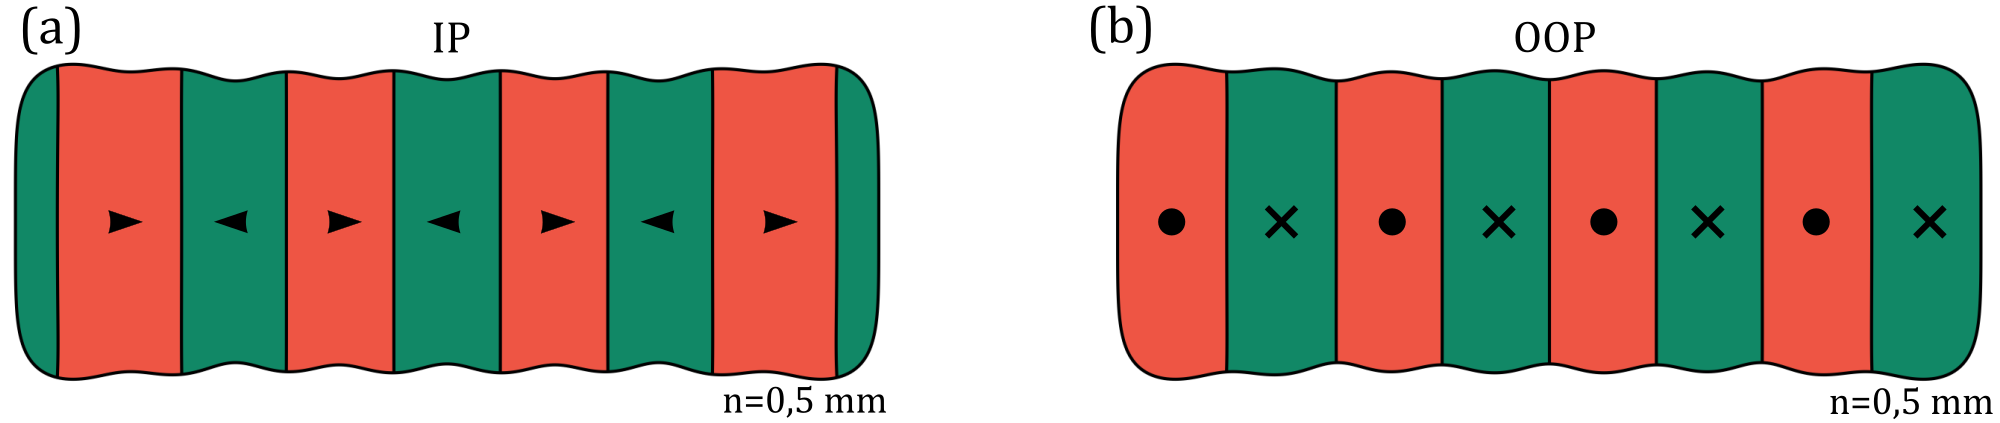
\includegraphics[width=1\linewidth,height=\textheight,keepaspectratio]{figures/sec05/07-feldprofil_ip_op.png}

}

\caption{\label{fig-sec05-07-feldprofil_ip_op}Felddarstellung von IP-
und OOP-Komponenten}

\end{figure}%

Abbildung~\ref{fig-sec05-07-feldprofil_ip_op} zeigt binäre
Felddarstellungen der in
Kapitel~\ref{sec-05-streufeld_einer_maßverkörperung} beschriebenen
Maßverkörperung auf einer \(p\)-\(o\)-Messfläche bei der Messhöhe
\(n = 0{,}5\,\mathrm{mm}\). Die Felddarstellungen sind jeweils auf den
durch den Amplitudengrenzwert \(B_G = 15\,\mathrm{mT}\) festgelegten
Nutzbereich beschränkt. Teilbild (a) zeigt die IP-Komponente \(B_p\),
Teilbild (b) die OOP-Komponente \(B_n\). Die Richtungssymbole sind
entsprechend der Darstellungskonvention ausgeführt.

Bei Felddarstellungen auf \(p\)-\(o\)-Messflächen nimmt die Messhöhe
\(n\) eine zentrale Stellung ein, da sie Lage und Form der dargestellten
Feldmerkmale wesentlich beeinflusst. Felddarstellungen werden aber
häufig in Aufsicht gezeigt, sodass sich der Abstand der Messfläche von
der Maßverkörperung aus der Darstellung nicht unmittelbar erschließen
lässt. Es wird daher empfohlen, die \textbf{Messhöhe unmittelbar in der
Felddarstellung anzugeben}, wie in
Abbildung~\ref{fig-sec05-07-feldprofil_ip_op} gezeigt. Diese Angabe
ermöglicht zugleich eine eindeutige Abgrenzung gegenüber der
Poldarstellung.

\begin{tcolorbox}[enhanced jigsaw, arc=.35mm, bottomrule=.15mm, bottomtitle=1mm, breakable, colback=white, colbacktitle=quarto-callout-tip-color!10!white, colframe=quarto-callout-tip-color-frame, coltitle=black, left=2mm, leftrule=.75mm, opacityback=0, opacitybacktitle=0.6, rightrule=.15mm, title=\textcolor{quarto-callout-tip-color}{\faLightbulb}\hspace{0.5em}{HINWEIS}, titlerule=0mm, toprule=.15mm, toptitle=1mm]

\emph{Die Poldarstellung sowie die Darstellung der Normalkomponente nach
Kapitel~\ref{sec-04-darstellungskonventionen} sind \textbf{Spezialfälle
der Felddarstellung}. Beide Darstellungen zeigen die OOP-Komponente des
Magnetfeldes auf der Oberfläche der Maßverkörperung (\(n = 0\)).}

\end{tcolorbox}

Eine Felddarstellung wird häufig auf die funktionale Oberfläche der
Maßverkörperung \textbf{projiziert}, um einen unmittelbaren örtlichen
Bezug zwischen Feldmerkmalen und Bauteilgeometrie herzustellen. Je nach
Bedarf kann sie dabei unabhängig von Amplitudengrenzen auf einen
\textbf{relevanten Ausschnitt} beschränkt werden.

\begin{figure}[h]

\centering{

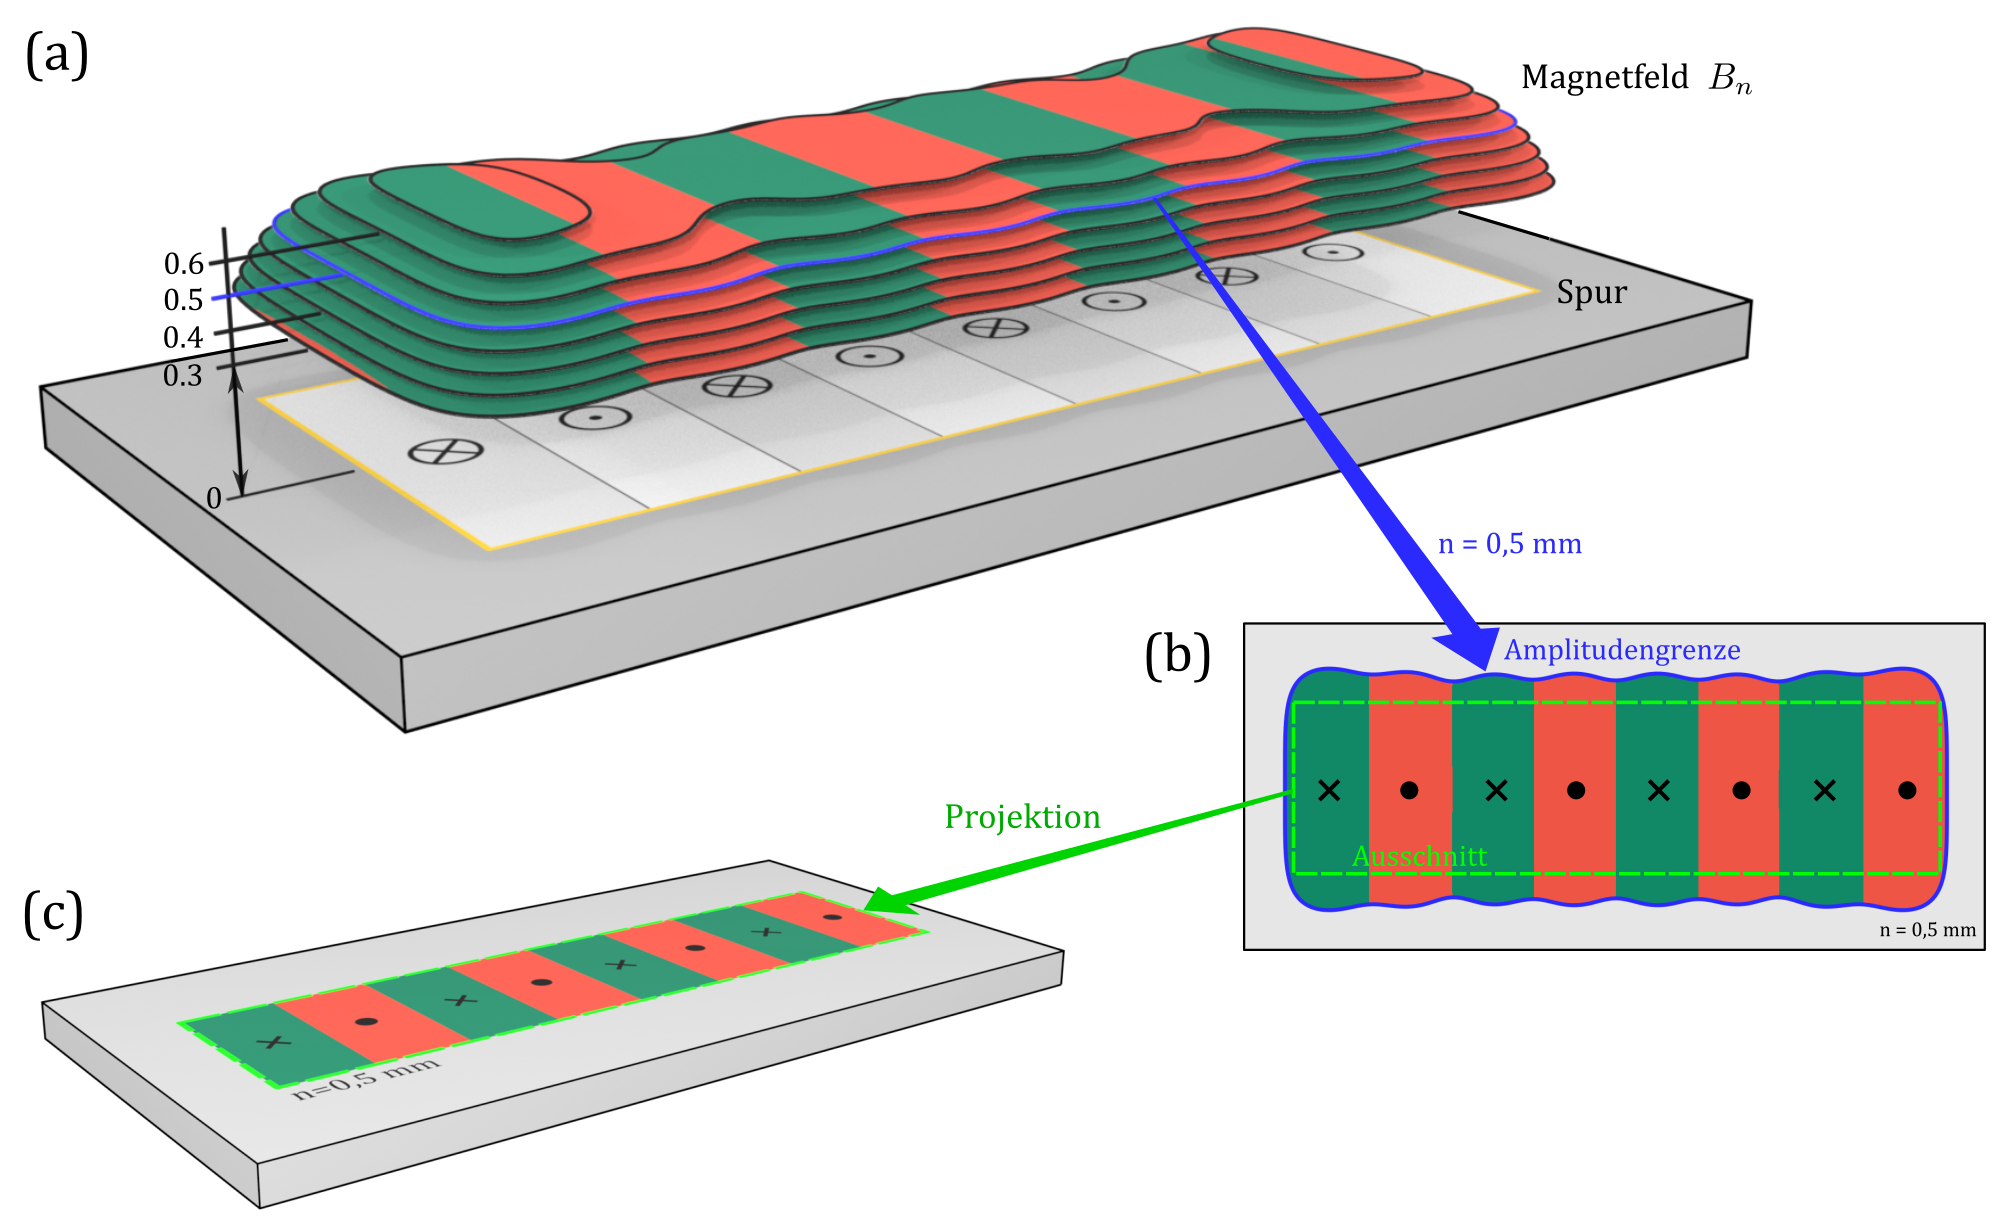
\includegraphics[width=1\linewidth,height=\textheight,keepaspectratio]{figures/sec05/08-felddarstellung_projektion.png}

}

\caption{\label{fig-sec05-08-felddarstellung_projektion}Felddarstellung
in Projektion auf die Maßverkörperung}

\end{figure}%

Abbildung~\ref{fig-sec05-08-felddarstellung_projektion} veranschaulicht
die Projektion einer Felddarstellung auf die funktionale Oberfläche der
Maßverkörperung. Teilbild (a) zeigt die in
Kapitel~\ref{sec-05-streufeld_einer_maßverkörperung} beschriebene
Maßverkörperung in Zonendarstellung. Darüber ist die aus einer
Simulation ermittelte Feldkomponente \(B_n\) auf mehreren, parallel zur
funktionalen Oberfläche angeordneten Messflächen binär dargestellt. Jede
Fläche ist dabei auf den Nutzbereich \(B > 15\,\mathrm{mT}\) beschränkt.
Der Abstand zwischen der Maßverkörperung und der untersten Messfläche
ist zur besseren Sichtbarkeit künstlich vergrößert.

Teilbild (b) zeigt die Messfläche bei \(n = 0{,}5\,\mathrm{mm}\) in
Aufsicht. Ein für die Anwendung relevanter Ausschnitt, beispielsweise
der Bereich der vorgesehenen Sensorpositionierung, ist hellgrün
strichliert umrahmt. Teilbild (c) zeigt die Maßverkörperung mit der auf
ihre funktionale Oberfläche projizierten Felddarstellung. Die Projektion
ist auf den in Teilbild (b) gekennzeichneten Ausschnitt beschränkt.

Die bisher gezeigten Felddarstellungen geben ermittelte Feldverläufe
konkreter Maßverkörperungen wieder und sind daher als
\textbf{Ist-Darstellungen} zu verstehen. Die Ermittlung kann durch
Messung oder durch Simulation erfolgen. An der Schnittstelle zwischen
Systemhersteller und Maßverkörperungshersteller werden Felddarstellungen
dagegen häufig als \textbf{Soll-Darstellungen} eingesetzt. Sie
beschreiben geforderte Feldverläufe und dienen der Spezifikation und
Kommunikation, ohne eine konkrete Realisierung vorauszusetzen.

\begin{figure}[h]

\centering{

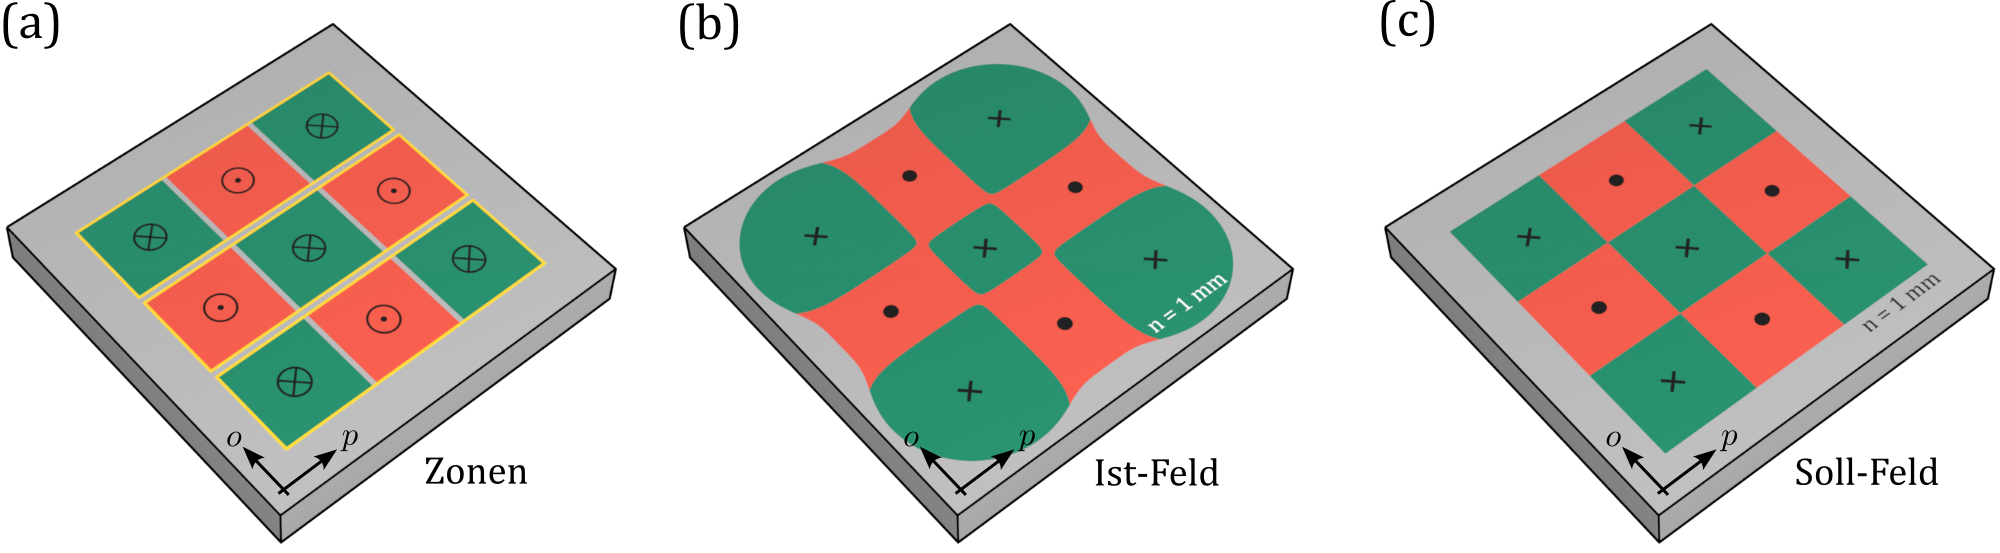
\includegraphics[width=1\linewidth,height=\textheight,keepaspectratio]{figures/sec05/09-felddarstellung_soll_ist.png}

}

\caption{\label{fig-sec05-09-felddarstellung_soll_ist}Felddarstellung
Soll und Ist}

\end{figure}%

Abbildung~\ref{fig-sec05-09-felddarstellung_soll_ist} zeigt ein
magnetisches Schachbrettmuster in verschiedenen Darstellungsformen.
Teilbild (a) zeigt die Maßverkörperung in farbcodierter
Zonendarstellung. Zu sehen ist eine graue Halterung mit eingepressten
kubischen Magneten, zwischen denen schmale Spalte erkennbar sind. Die
Magnete bilden drei parallele Spuren. Die Darstellung beschreibt den
strukturellen Aufbau und die Anordnung der magnetisierten Zonen.

Teilbild (b) zeigt eine Ist-Felddarstellung in binärer Form. Sie ist auf
einen amplitudenbezogenen Nutzbereich beschränkt und auf die
Maßverkörperung projiziert. Der zugrunde liegende Feldverlauf wurde
durch Simulation des Magnetfeldes der in Teilbild (a) gezeigten
Maßverkörperung auf einer \(p\)-\(o\)-Messfläche bei der Messhöhe
\(n = 1\,\mathrm{mm}\) ermittelt.

Teilbild (c) zeigt eine Soll-Felddarstellung in binärer Form. Sie stellt
weder einen Ausschnitt des in Teilbild (b) dargestellten Feldverlaufs
noch das Ergebnis einer Messung oder Simulation dar. Vielmehr dient sie
der Beschreibung gewünschter Feldmerkmale und könnte beispielsweise eine
Bedarfsanforderung oder Zielvorgabe für die Auslegung einer
Maßverkörperung repräsentieren.

\begin{tcolorbox}[enhanced jigsaw, arc=.35mm, bottomrule=.15mm, bottomtitle=1mm, breakable, colback=white, colbacktitle=quarto-callout-tip-color!10!white, colframe=quarto-callout-tip-color-frame, coltitle=black, left=2mm, leftrule=.75mm, opacityback=0, opacitybacktitle=0.6, rightrule=.15mm, title=\textcolor{quarto-callout-tip-color}{\faLightbulb}\hspace{0.5em}{HINWEIS}, titlerule=0mm, toprule=.15mm, toptitle=1mm]

\emph{Die vorgestellten \textbf{Darstellungsformen} können sich in ihrer
grafischen Erscheinung stark ähneln, unterscheiden sich jedoch
grundlegend hinsichtlich ihrer Bedeutung und ihres Informationsgehalts.
Bei der \textbf{Interpretation} ist besonders darauf zu achten, welche
Darstellungsform vorliegt.}

\end{tcolorbox}

\section{Spurfelder}\label{sec-05-spurfelder}

Die bisherigen Unterkapitel beschreiben das Streufeld einer
Maßverkörperung unabhängig von einer Gliederung der magnetischen
Struktur in Spuren. Bei magnetischen Maßstäben mit mehreren Spuren wird
das von einer einzelnen Spur erzeugte Magnetfeld als \textbf{Spurfeld}
bezeichnet. Das gesamte Streufeld des Maßstabs ergibt sich aus der
Überlagerung der einzelnen Spurfelder.

Bei der Vermessung einer Spur ist auf den \textbf{Einfluss benachbarter
Spurfelder} zu achten, da experimentell grundsätzlich das Gesamtfeld
erfasst wird. In vielen praktischen Anwendungen wird deshalb der
Spurabstand so gewählt, dass dieser Einfluss gering bleibt. Dies wird
durch den raschen Abfall der Spurfelder über die seitlichen Begrenzungen
der jeweiligen Spur hinaus begünstigt. Bei geeignet gewähltem
Spurabstand können die Nutzbereiche, die aus dem Gesamtfeld ermittelt
werden, räumlich voneinander getrennt sein und den darunterliegenden
Spuren eindeutig zugeordnet werden.

\begin{figure}[h]

\centering{

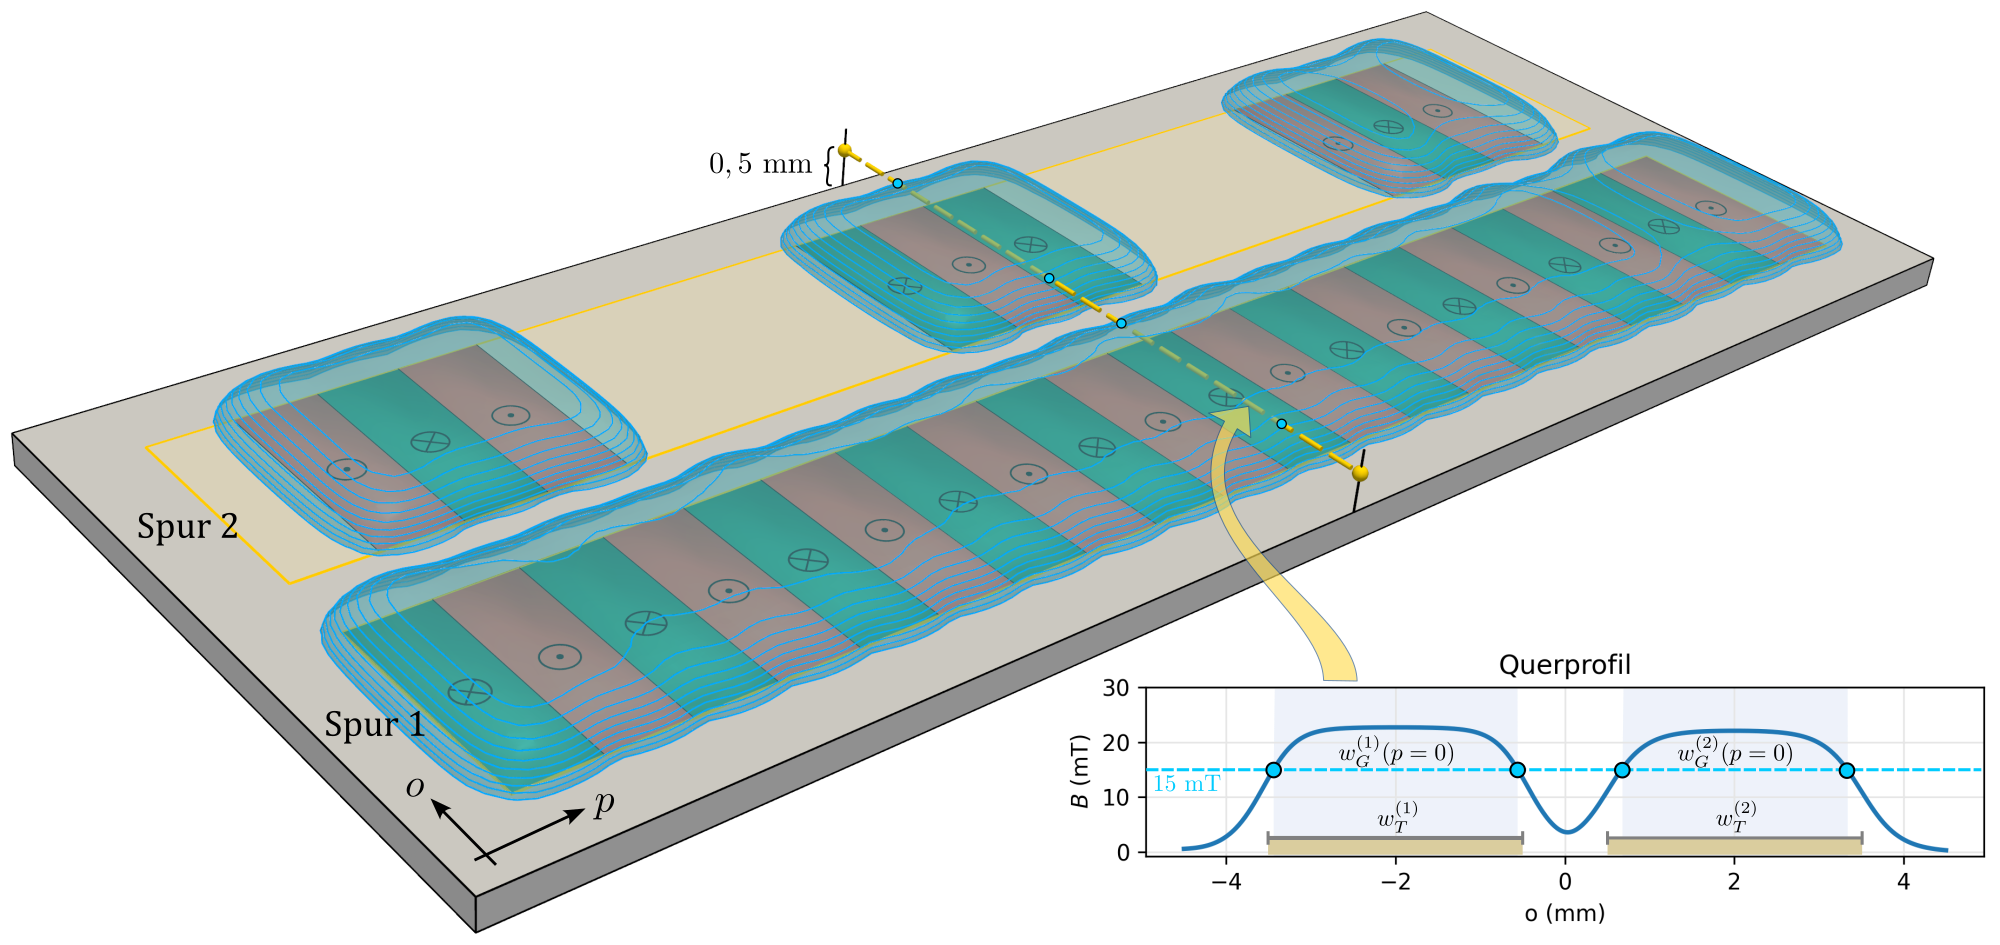
\includegraphics[width=1\linewidth,height=\textheight,keepaspectratio]{figures/sec05/10-spurfeld.png}

}

\caption{\label{fig-sec05-10-spurfeld}Spurfelder und Nutzbereiche
mehrspuriger Maßstäbe}

\end{figure}%

Abbildung~\ref{fig-sec05-10-spurfeld} zeigt die Simulation eines
magnetischen Maßstabs mit zwei parallelen OOP-polarisierten
Linearspuren: einer vollbeschriebenen Inkrementalspur und einer
segmentierten Spur mit drei Referenzbereichen. In der Simulation wurden
die Zonen als homogen, mit einer Polarisation von
\(J_Z = 350\,\mathrm{mT}\) modelliert. Die Spurbreiten betragen
\(w_T = 3\,\mathrm{mm}\), der Spurabstand \(w_{TT} = 1\,\mathrm{mm}\).
Die Zonenlängen betragen \(\ell_Z = 1\,\mathrm{mm}\) und die Zonentiefe
\(d_Z = 200\,\mu\mathrm{m}\). Die für den Amplitudengrenzwert
\(B_G = 15\,\mathrm{mT}\) ermittelten Nutzbereiche sind durch ihre
Amplitudengrenzflächen als blaue, blasenförmige Hüllflächen über dem
Maßstab dargestellt.

Das Querprofil der Feldamplitude \(|\vec{B}|\) entlang des
eingezeichneten \(o\)-Pfades bei einer Messhöhe von
\(0{,}5\,\mathrm{mm}\) ist in einem Teilbild gezeigt. Aufgrund des
starken seitlichen Abfalls der Feldamplitude über die Spuren hinaus
ergeben sich unter den gewählten Ermittlungsbedingungen voneinander
\textbf{getrennte Nutzbereiche}. Das Querprofil zeigt, dass die
Nutzbereichsbreiten \(w_G\) bei dieser Messhöhe für beide Spuren
geringer sind als die jeweiligen Spurbreiten \(w_T\).

Wie in der Abbildung erkennbar, hängen Lage und Abmessungen der
Nutzbereiche wesentlich von den zugrunde liegenden Zonenmustern ab. Der
vollbeschriebenen Inkrementalspur ist ein langer, zusammenhängender
Nutzbereich zugeordnet. Der segmentierten Spur sind dagegen drei
voneinander getrennte Nutzbereiche zugeordnet, die über den drei
Referenzbereichen liegen. Besitzt eine Spur \textbf{mehrere
Nutzbereiche}, werden diese, beginnend mit 1, entlang der positiven
\(p\)-Richtung fortlaufend nummeriert.

\bookmarksetup{startatroot}

\chapter{Grundlagen der Vermessung}\label{sec-06}

Aufbauend auf der Beschreibung von Geometrie und Anordnung des
Messsystems in Kapitel~\ref{sec-03}, der magnetischen Struktur in
Kapitel~\ref{sec-04} sowie des Streufeldes in Kapitel~\ref{sec-05}
behandelt dieses Kapitel Grundlagen der Vermessung magnetischer
Maßverkörperungen. Im Mittelpunkt stehen dabei die Messgrößen,
Bezugssysteme und sensorunabhängigen Größen der Ermittlung und
Auswertung.

\section{Messgegenstand}\label{sec-06-messgegenstand}

Die \textbf{magnetische Struktur} nach Kapitel~\ref{sec-04} wird in der
Praxis typischerweise \textbf{nicht vermessen}. Die experimentelle
Ermittlung des Zonenmusters ist nur mit speziellen Verfahren und hohem
messtechnischen Aufwand möglich. Auch das Polmuster ist nicht
unmittelbar zugänglich, da es die Normalkomponente des Streufeldes
direkt an der physischen Oberfläche der Maßverkörperung bei \(n = 0\)
beschreibt, was den Einsatz realer Magnetfeldsensoren mit endlichen
Abmessungen verhindert.

Die magnetische Vermessung von Maßverkörperungen beschränkt sich im
Allgemeinen auf die \textbf{Erfassung und Auswertung ihres Streufeldes}
in einer endlichen Messhöhe. Dazu werden Magnetfeldsensoren in
entsprechenden Ermittlungsbereichen bewegt. Für Weg- und
Winkelmesssysteme handelt es sich dabei meist um \(p\)-Messpfade und
\(p\)-\(o\)-Messflächen bei Messhöhen, die in der Größenordnung einer
halben bis weniger Pollängen liegen. Bei diesen Messhöhen ist die
Feldamplitude typischerweise noch ausreichend groß für die Sensorik,
während höhere räumliche Harmonische der betrachteten Feldkomponente
bereits weniger ausgeprägt sind.

Unmittelbar \textbf{experimentell erfasst} werden die Komponenten des
Magnetfeldes. Aus den resultierenden Feldverläufen können Feldmerkmale
wie Nullstellen, Peaks, Amplituden- und Nutzbereichsgrenzen, Halbwellen,
magnetische Perioden sowie weitere Eigenschaften des Streufeldes
abgeleitet werden.

Die ermittelten Feldgrößen sind stets gemeinsam mit den zugehörigen
\textbf{Ermittlungsbedingungen} anzugeben. Dazu zählen insbesondere die
betrachtete Feldkomponente oder Feldamplitude, die Messhöhe, Lage und
Orientierung des Ermittlungsbereichs sowie gegebenenfalls der verwendete
Amplitudengrenzwert. Eigenschaften des eingesetzten Prüfsystems können
das Messergebnis zusätzlich beeinflussen, sind jedoch nicht Gegenstand
der in diesem Kapitel diskutierten sensorunabhängigen Ermittlungs- und
Auswerteprozeduren.

\begin{tcolorbox}[enhanced jigsaw, arc=.35mm, bottomrule=.15mm, bottomtitle=1mm, breakable, colback=white, colbacktitle=quarto-callout-tip-color!10!white, colframe=quarto-callout-tip-color-frame, coltitle=black, left=2mm, leftrule=.75mm, opacityback=0, opacitybacktitle=0.6, rightrule=.15mm, title=\textcolor{quarto-callout-tip-color}{\faLightbulb}\hspace{0.5em}{HINWEIS}, titlerule=0mm, toprule=.15mm, toptitle=1mm]

\emph{Die experimentell ermittelten Größen beziehen sich auf das
Streufeld nach Kapitel~\ref{sec-05} und sind von den Strukturgrößen nach
Kapitel~\ref{sec-04} zu unterscheiden. Eine \textbf{begriffliche
Zuordnung} wird in Kapitel~\ref{sec-06-strukturbegriffe-feldgroessen}
behandelt.}

\end{tcolorbox}

\section{Mechanischer Bezug}\label{sec-06-mech_bezug}

Für die eindeutige Beschreibung der Lage magnetischer Strukturen und
Feldmerkmale gegenüber der Bauteilgeometrie ist ein reproduzierbarer
\textbf{mechanischer Bezug} erforderlich. Dieser wird durch ein
mechanisches Datumssystem der Maßverkörperung festgelegt.

Das \textbf{Datumssystem} wird nach ISO 5459:2024 ausschließlich aus
geometrischen Datumsmerkmalen der Maßverkörperung abgeleitet,
beispielsweise aus Flächen, Kanten, Achsen oder geeigneten Markierungen.
Es beschreibt damit die mechanische Lage und Orientierung der
Maßverkörperung unabhängig von ihren magnetischen Eigenschaften. Die
Wahl des Datumssystems sollte sich nach den für Herstellung, Montage und
Vermessung relevanten geometrischen Bezugsmerkmalen richten.

Der \textbf{Koordinatenursprung} der Maßverkörperung \(O_M\) wird aus
diesem Datumssystem abgeleitet. Gemeinsam mit der Orientierung der
Koordinatenrichtungen nach
Kapitel~\ref{sec-03-koordinatensystem_der_maßverkörperung} können damit
die magnetische Struktur und das Streufeld auf die experimentell
ermittelte Bauteilgeometrie bezogen werden.

\begin{figure}[h]

\centering{

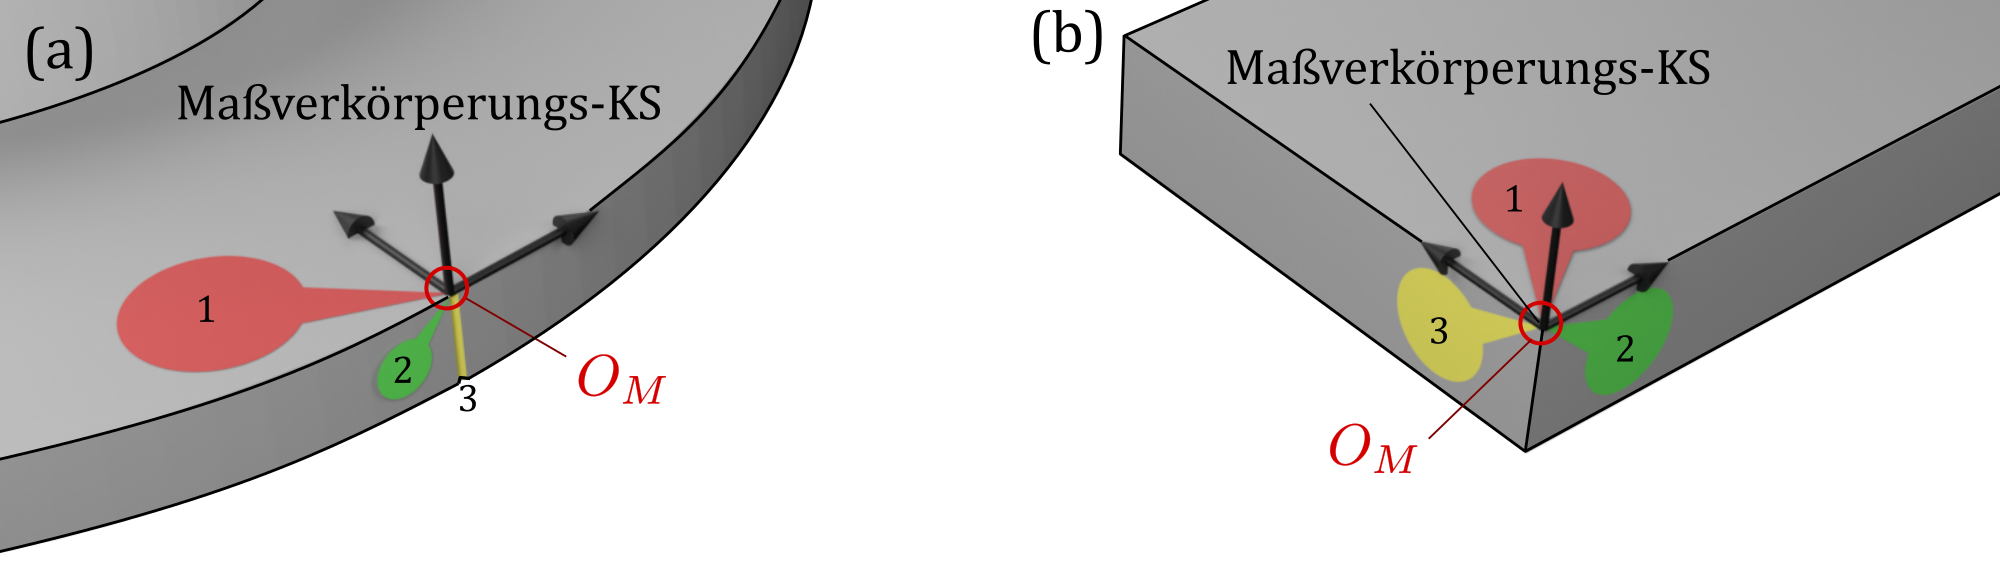
\includegraphics[width=0.8\linewidth,height=\textheight,keepaspectratio]{figures/sec06/01-mech_bezug.png}

}

\caption{\label{fig-sec06-01-mech_bezug}Mechanischer Bezug}

\end{figure}%

Abbildung~\ref{fig-sec06-01-mech_bezug} zeigt zwei Beispiele zur
Ableitung des Koordinatenursprungs \(O_M\) aus geometrischen
Datumssystemen. Teilbild (a) zeigt eine rotationssymmetrische
Maßverkörperung, deren Datumssystem durch die Oberseite (rot), die
Mantelfläche (grün) und eine Markierung auf der Mantelfläche (gelb)
festgelegt ist. Teilbild (b) zeigt eine quaderförmige Maßverkörperung,
bei der das Datumssystem aus drei orthogonalen Seitenflächen abgeleitet
wird. Die Datumselemente können beispielsweise mit taktilen oder
optischen Messverfahren ermittelt werden. Die farbliche Hervorhebung in
der Abbildung dient ausschließlich ihrer besseren Unterscheidbarkeit.

\section{Magneto-mechanischer Bezug und
Feld-KS}\label{sec-06-mag_mech_bezug}

Die \textbf{Vermessung des Streufeldes} erfolgt grundsätzlich in Bezug
auf die Geometrie und Lage der Maßverkörperung. Die Beschreibung der
Ermittlungsbereiche für die Vermessung kann auf das Maßverkörperungs-KS
bezogen werden, für das ein mechanischer Bezug nach
Kapitel~\ref{sec-06-mech_bezug} besteht. Ein Struktur-KS ist hierfür
nicht geeignet, da dessen Lage aus Strukturgrößen abgeleitet wird, die
nicht unmittelbar vermessen werden können.

Die genaue Herstellung des mechanischen Bezugs sowie die präzise
Sensorpositionierung relativ zur Maßverkörperung können jedoch mit hohem
Aufwand verbunden sein. Gleichzeitig ist für viele Anwendungen die
absolute Lage der Feldmerkmale gegenüber der Bauteilgeometrie von
geringerer Bedeutung als ihre \textbf{präzise relative Lage} zueinander.

Für die Vermessung empfiehlt es sich deshalb, ein \textbf{Feld-KS} zu
verwenden, dessen Ursprung \(O_F\) anhand ausgewählter Feldmerkmale
festgelegt wird. Die Koordinatenrichtungen des Feld-KS entsprechen den
lokalen \(p\)-, \(o\)- und \(n\)-Richtungen des Maßverkörperungs-KS.
Gemeinsam mit den Richtungsvektoren \(\vec{e}_p\), \(\vec{e}_o\) und
\(\vec{e}_n\) definiert \(O_F\) das Feld-KS.

Das Feld-KS ermöglicht eine Beschreibung der Feldmerkmale, die
unmittelbar \textbf{aus der Vermessung ableitbar} ist. Es berücksichtigt
besonders die anwendungsrelevanten relativen Lagen der Feldmerkmale und
erleichtert den Vergleich gleichartiger Maßverkörperungen.

Ist das Feld-KS einem Spurfeld zugeordnet, wird es als
\textbf{Spurfeld-KS} bezeichnet. Besitzt ein magnetischer Maßstab
mehrere Spuren, sollte jedem Spurfeld ein eigenes Spurfeld-KS zugeordnet
werden. Besitzt eine Spur mehrere voneinander getrennte Nutzbereiche,
werden diese in einem gemeinsamen Spurfeld-KS beschrieben.

Als \textbf{Referenzlagen für den Ursprung} \(O_F\) werden
typischerweise in \(p\)-Richtung die Nullstelle 1 und in \(o\)-Richtung
die Mitte des zugehörigen Nutzbereichs verwendet. In \(n\)-Richtung wird
\(O_F\) üblicherweise auf die funktionale Oberfläche der Maßverkörperung
gelegt.

Die Lage von \(O_F\) im Maßverkörperungs-KS bildet den
\textbf{magneto-mechanischen Bezug}, der das vermessene Streufeld mit
der Bauteilgeometrie in Bezug setzt. Für die praktische Ermittlung
sollte die ungefähre Lage von \(O_F\) durch mechanische Merkmale,
beispielsweise Bauteilkanten oder Markierungen, bekannt sein. Die genaue
Lage kann anschließend durch Vermessung des Streufeldes in deren
Umgebung bestimmt werden.

\begin{figure}[h]

\centering{

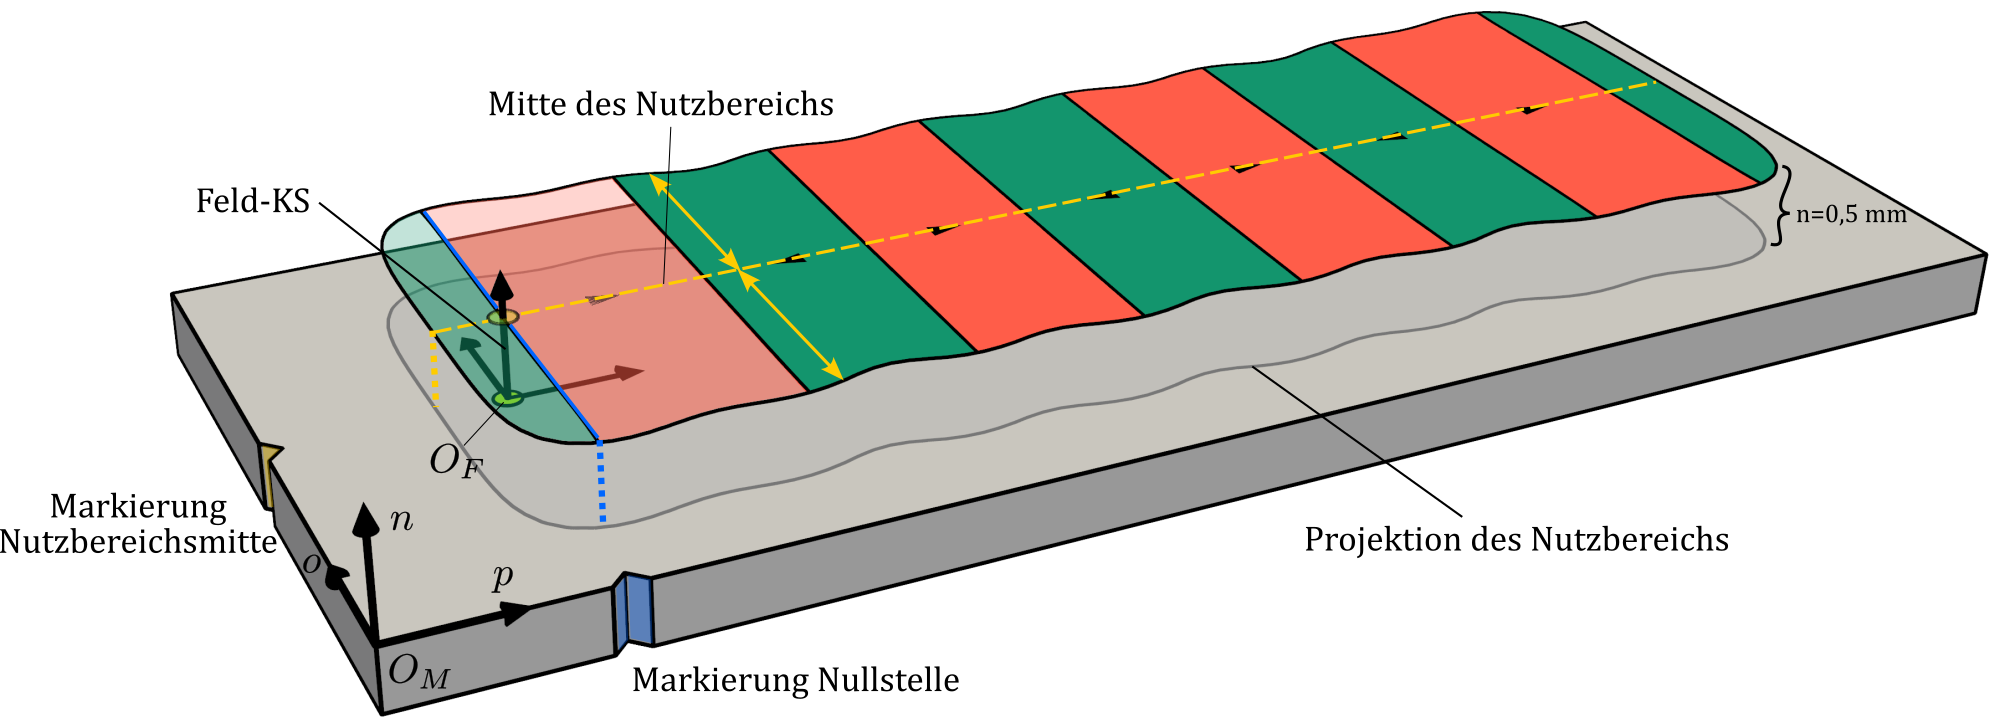
\includegraphics[width=1\linewidth,height=\textheight,keepaspectratio]{figures/sec06/02-mag_mech_bezug.png}

}

\caption{\label{fig-sec06-02-mag_mech_bezug}Magneto-mechanischer Bezug
und Feld-KS}

\end{figure}%

Abbildung~\ref{fig-sec06-02-mag_mech_bezug} veranschaulicht den
magneto-mechanischen Bezug und die Ermittlung eines Feld-KS. Dargestellt
sind die Maßverkörperung aus
Kapitel~\ref{sec-05-streufeld_einer_maßverkörperung} und darüber liegend
eine binäre Felddarstellung der IP-Komponente des Streufeldes, das auf
einer \(p\)-\(o\)-Messfläche bei einer Messhöhe von
\(n = 0{,}5\,\mathrm{mm}\) ermittelt wurde. Die Felddarstellung ist
dabei auf den durch den Amplitudengrenzwert \(B_G = 15\,\mathrm{mT}\)
festgelegten Nutzbereich beschränkt.

In der Abbildung ist der Ursprung des Feld-KS in \(p\)-Richtung durch
die erste Nullstelle (blau), in \(o\)-Richtung durch die Mitte des
Nutzbereichs (gelb) und in \(n\)-Richtung durch die funktionale
Oberfläche der Maßverkörperung festgelegt. Markierungen an der Seite der
Maßverkörperung zeigen die ungefähre Lage der ersten Nullstelle und der
Mitte des Nutzbereichs an. Zur besseren Sichtbarkeit des
Koordinatenkreuzes des Feld-KS, das auf der funktionalen Oberfläche der
Maßverkörperung liegt, sind die ersten beiden Halbwellen der
Felddarstellung transparent ausgeführt.

\begin{tcolorbox}[enhanced jigsaw, arc=.35mm, bottomrule=.15mm, bottomtitle=1mm, breakable, colback=white, colbacktitle=quarto-callout-tip-color!10!white, colframe=quarto-callout-tip-color-frame, coltitle=black, left=2mm, leftrule=.75mm, opacityback=0, opacitybacktitle=0.6, rightrule=.15mm, title=\textcolor{quarto-callout-tip-color}{\faLightbulb}\hspace{0.5em}{HINWEIS}, titlerule=0mm, toprule=.15mm, toptitle=1mm]

\emph{Das \textbf{Feld-KS} ist grundsätzlich gleich aufgebaut wie das
\textbf{Struktur-KS} nach Kapitel~\ref{sec-04-darstellungskonventionen}.
Sie unterscheiden sich in der Festlegung des Ursprungs und in ihrem
Verwendungszweck. Der Ursprung \(O_T\) wird anhand der magnetischen
Strukturmerkmale festgelegt. Das Struktur-KS dient der Beschreibung der
magnetischen Struktur einer Maßverkörperung. Der Ursprung \(O_F\) wird
dagegen anhand von Feldmerkmalen festgelegt. Das Feld-KS dient der
Vermessung des Streufeldes.}

\end{tcolorbox}

\section{Spurfeldlage und
-abmessungen}\label{sec-06-spurfeldlage_abmessungen}

Bei mehrspurigen Maßstäben werden die nachfolgend beschriebenen
Spurfeldgrößen aus den dem jeweiligen Spurfeld zugeordneten Bereichen
des gemessenen Gesamtfeldes bestimmt.

Um mehrere Spurfelder räumlich zueinander in Bezug zu setzen, wird die
\textbf{Spurfeldlage} \(\vec{r}_F^{(i)}\) als Lage des Ursprungs
\(O_F^{(i)}\) des \(i\)-ten Spurfeld-KS im Maßverkörperungs-KS
festgelegt. Ihre Koordinaten sind \(p_F^{(i)}\), \(o_F^{(i)}\) und
\(n_F^{(i)}\). Da \(O_F^{(i)}\) auf der funktionalen Oberfläche liegt,
gilt \(n_F^{(i)} = 0\).

Die relative Lage zweier Spurfelder wird durch ihre Versätze
beschrieben. Als \textbf{Spurfeld-Längsversatz} \(p_{FF}\) wird der
Versatz in \(p\)-Richtung bezeichnet. Es gilt

\[
p_{FF}^{(i_1,i_2)} = p_F^{(i_2)} - p_F^{(i_1)}.
\]

Der \textbf{Spurfeld-Querversatz} \(o_{FF}\) bezeichnet entsprechend den
Versatz in \(o\)-Richtung,

\[
o_{FF}^{(i_1,i_2)} = o_F^{(i_2)} - o_F^{(i_1)}.
\]

Da sich ein Versatz auf zwei Spurfelder bezieht, wird nach
Indexkonvention in Kapitel~\ref{sec-03-indexkonvention} das Kürzel „FF``
für den Bezugsindex verwendet.

\begin{figure}[h]

\centering{

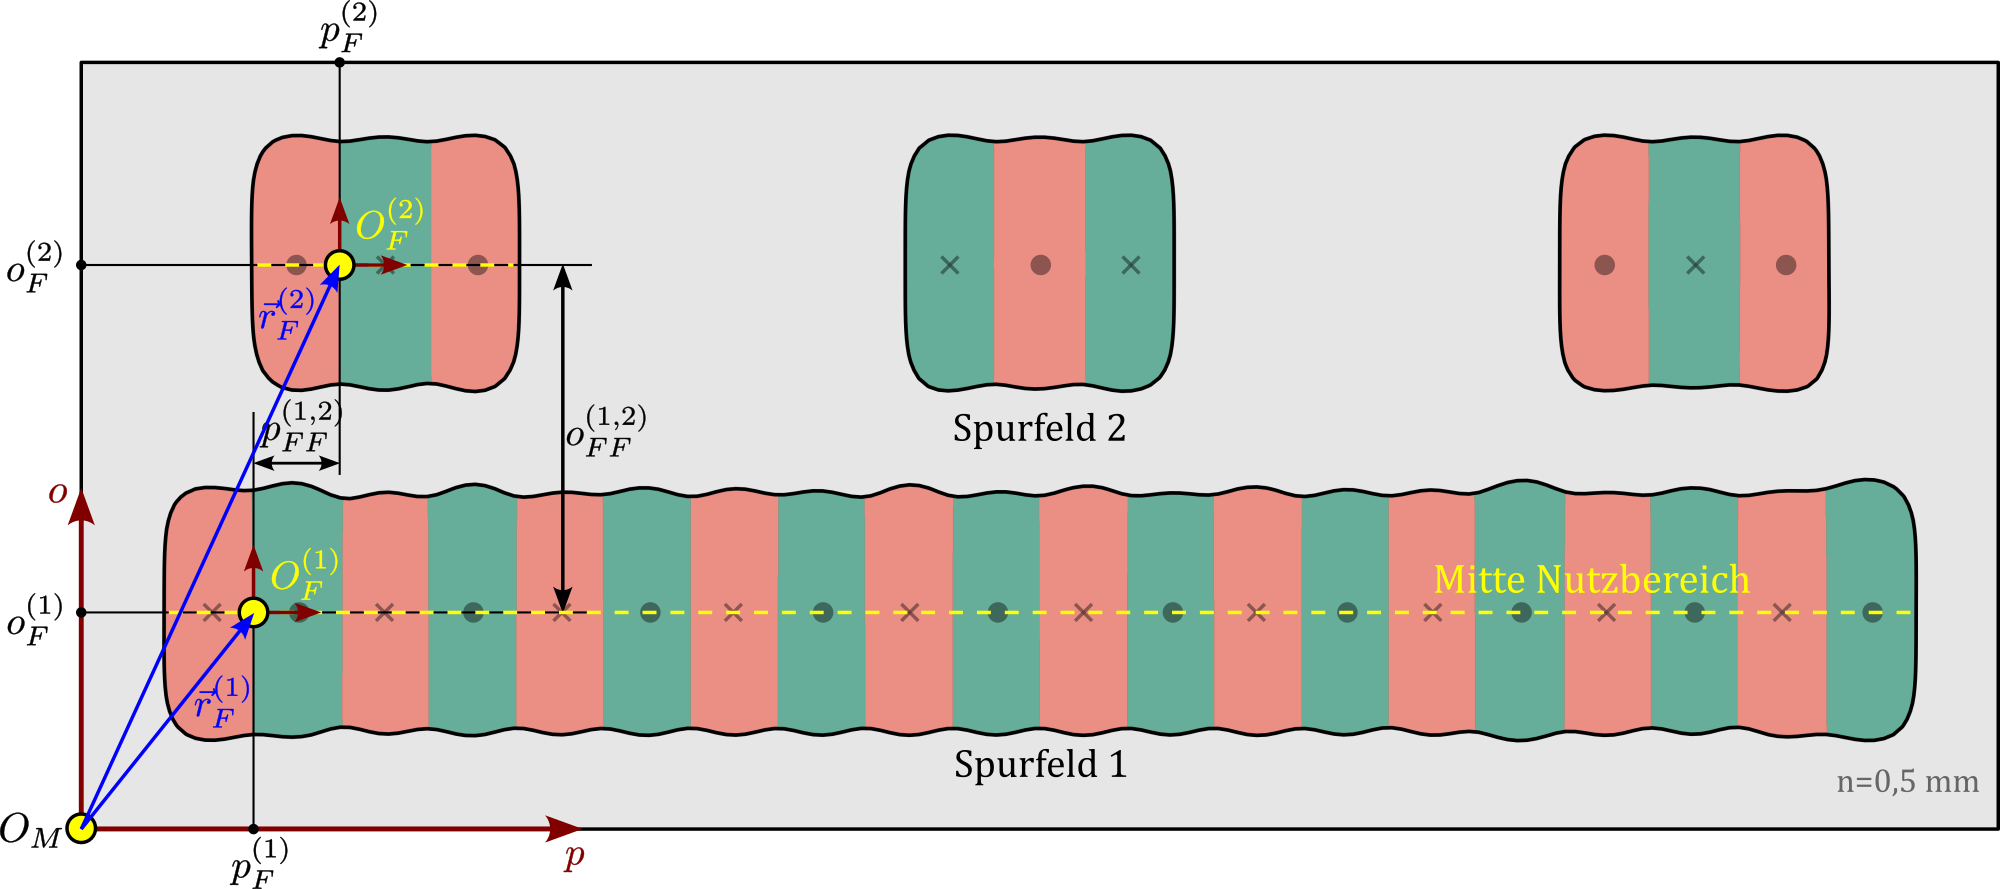
\includegraphics[width=1\linewidth,height=\textheight,keepaspectratio]{figures/sec06/03-spurfeldlage.png}

}

\caption{\label{fig-sec06-03-spurfeldlage}Spurfeldlage}

\end{figure}%

Abbildung~\ref{fig-sec06-03-spurfeldlage} zeigt den in
Abbildung~\ref{fig-sec05-10-spurfeld} dargestellten magnetischen Maßstab
in Aufsicht. Die Nutzbereiche bei einer Messhöhe von
\(n = 0{,}5\,\mathrm{mm}\) sind auf die funktionale Oberfläche des
Maßstabs projiziert. Innerhalb der Nutzbereiche ist die
\(B_n\)-Komponente des Magnetfeldes in binärer Darstellung
wiedergegeben.

Für jede Spur ist ein zugehöriges Spurfeld-KS eingezeichnet. Die
Ursprünge \(O_F^{(1)}\) und \(O_F^{(2)}\) werden im Maßverkörperungs-KS
durch die blau eingezeichneten Spurfeldlagen \(\vec{r}_F^{(1)}\) und
\(\vec{r}_F^{(2)}\) beschrieben. Im dargestellten Beispiel werden ihre
Lagen in \(p\)-Richtung durch die jeweils erste Nullstelle und in
\(o\)-Richtung durch die Mitte des zugehörigen Nutzbereichs (gelb)
festgelegt.

Die \textbf{Abmessungen eines Spurfeldes} werden aus den Abmessungen
seiner Nutzbereiche abgeleitet. Dabei ist in \(p\)-Richtung nicht die
gesamte räumliche Ausdehnung eines Nutzbereichs maßgebend, sondern nur
der Bereich, in dem für die jeweilige Anwendung ein nutzbares Spurfeld
erforderlich ist.

Dazu werden entlang einer Spur ein oder mehrere
\textbf{Betriebsabschnitte} festgelegt. Sie bezeichnen zusammenhängende
Bereiche in \(p\)-Richtung, innerhalb derer das Spurfeld bewertet wird.
Die Ermittlung der Spurfeldabmessungen erfolgt ausschließlich innerhalb
dieser Betriebsabschnitte.

Da die Nutzbereichsbreite \(w_G(p)\) innerhalb der Betriebsabschnitte
variieren kann, wird die \textbf{Spurfeldbreite} \(w_F\) als die
kleinste Nutzbereichsbreite innerhalb aller Betriebsabschnitte einer
Spur festgelegt. Die für den magneto-mechanischen Bezug genutzte
\textbf{Mitte des Nutzbereichs} sollte sich auf diese kleinste
Nutzbereichsbreite beziehen. Eine entsprechende Spurfeldlänge wird nicht
definiert, da die relevante Ausdehnung in \(p\)-Richtung bereits durch
die Betriebsabschnitte festgelegt ist.

Der sich aus den Spurfeldbreiten und dem Spurfeld-Querversatz ergebende
Abstand zwischen zwei benachbarten, räumlich getrennten Spurfeldern wird
als \textbf{Spurfeldabstand} \(w_{FF}\) bezeichnet. Es gilt:

\[
w_{FF}^{(i_1,i_2)}
=
\left|o_{FF}^{(i_1,i_2)}\right|
-
\frac{w_F^{(i_1)} + w_F^{(i_2)}}{2}
\]

Die folgende Abbildung~\ref{fig-sec06-04-spurfeldbreite} zeigt den
magnetischen Maßstab aus Abbildung~\ref{fig-sec06-03-spurfeldlage} in
Aufsicht. Zusätzlich wurde ein Materialdefekt simuliert, der im
ausgewiesenen Bereich zu einer Verringerung der Polarisation auf
\(80\,\%\) ihres ursprünglichen Wertes führt.

\begin{figure}[h]

\centering{

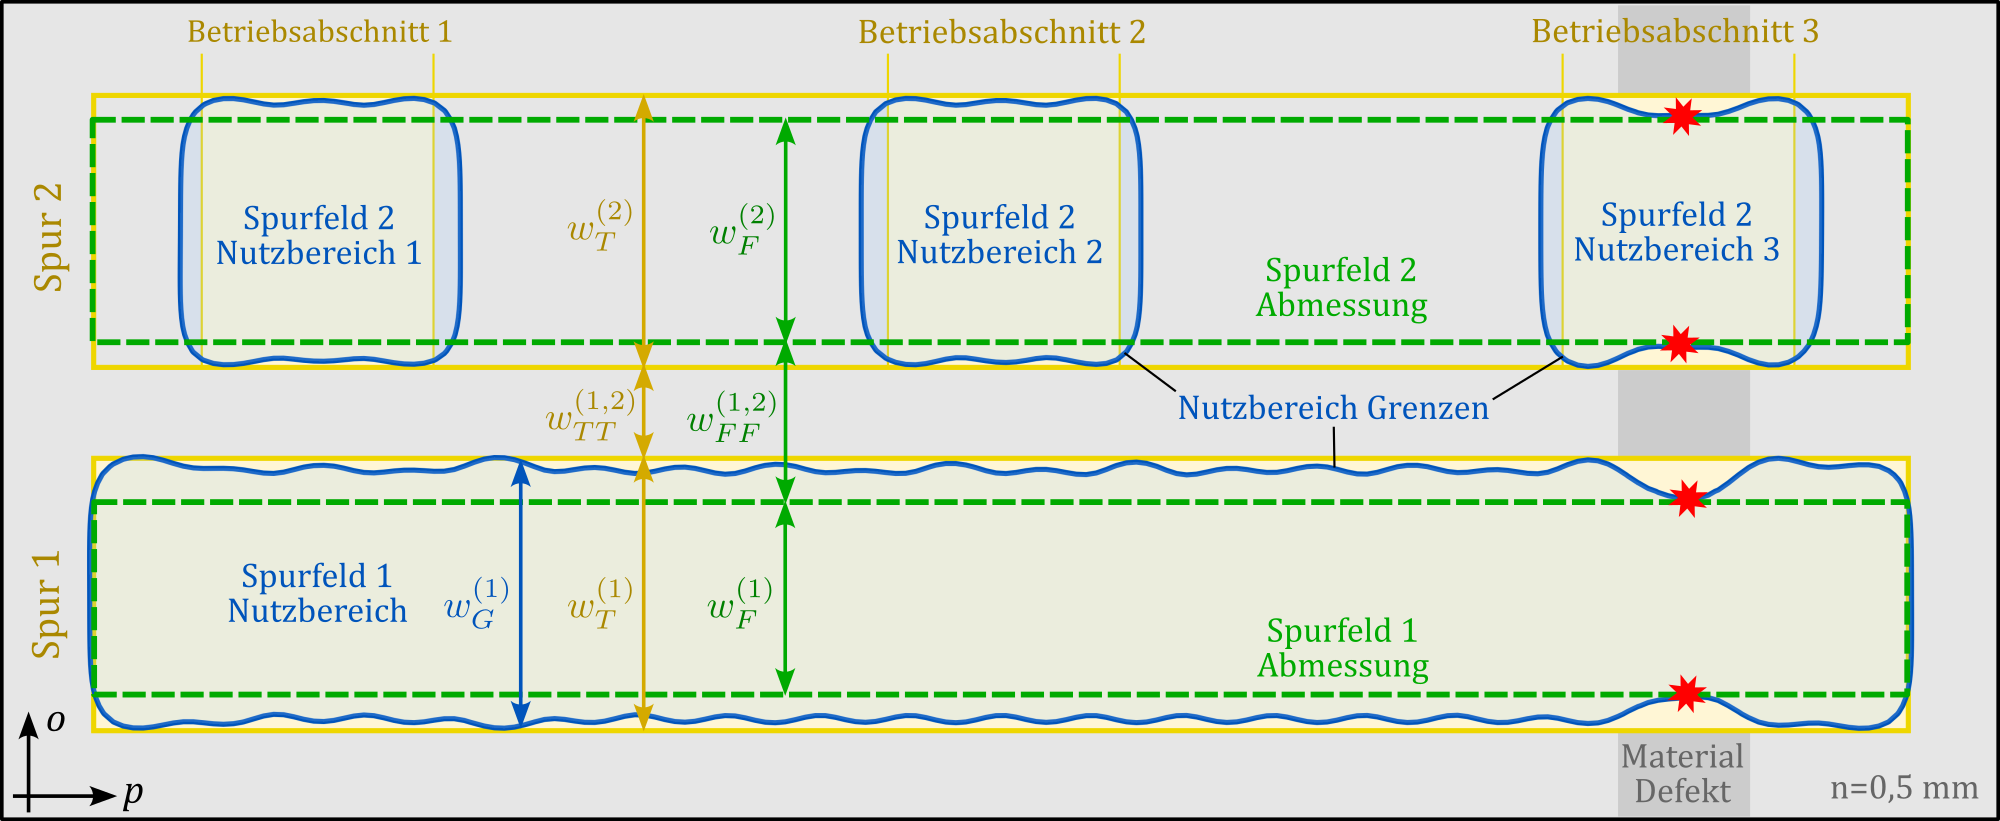
\includegraphics[width=1\linewidth,height=\textheight,keepaspectratio]{figures/sec06/04-spurfeldbreite.png}

}

\caption{\label{fig-sec06-04-spurfeldbreite}Spurbreite und
Spurfeldbreite}

\end{figure}%

In der Abbildung sind die Nutzbereiche bei einer Messhöhe von
\(n = 0{,}5\,\mathrm{mm}\) auf die funktionale Oberfläche des Maßstabs
projiziert und blau dargestellt. Die darunterliegenden Spuren sind gelb
umrandet; ihre Betriebsabschnitte sind gelb ausgefüllt.

Die \textbf{Spurfeldbreite} ergibt sich aus der kleinsten
Nutzbereichsbreite innerhalb der Betriebsabschnitte. Die Positionen, an
denen diese Mindestbreiten auftreten, sind durch rote Sterne markiert.
Die sich daraus ergebenden feldbezogenen Spurabmessungen sind grün
strichliert umrandet. Breiten und Abstände von Nutzbereich (lokal), Spur
und Spurfeld sind entsprechend eingezeichnet.

\begingroup
\footnotesize
\renewcommand{\baselinestretch}{1.12}\selectfont
\setlength{\tabcolsep}{5pt}
\setlength{\extrarowheight}{2.5pt}
\renewcommand{\arraystretch}{1.15}
{\begin{longtable}[]{
  >{\raggedright\arraybackslash}p{(\linewidth - 4\tabcolsep) * \real{0.2600}}
  >{\centering\arraybackslash}p{(\linewidth - 4\tabcolsep) * \real{0.1500}}
  >{\raggedright\arraybackslash}p{(\linewidth - 4\tabcolsep) * \real{0.5900}}}
\caption{Begriffe Spurfeld}\label{tbl-begriffe-spurfeld}\tabularnewline
\arrayrulecolor{tableouterrule}
\toprule\noalign{}
\rowcolor{zebrabluehead}
\begin{minipage}[b]{\linewidth}\raggedright
\textbf{Begriff}
\end{minipage} & \begin{minipage}[b]{\linewidth}\centering
\textbf{Symbol}
\end{minipage} & \begin{minipage}[b]{\linewidth}\raggedright
\textbf{Beschreibung}
\end{minipage} \\
\arrayrulecolor{tableheadrule}
\specialrule{0.35pt}{0pt}{0pt}
\endhead
\arrayrulecolor{tableouterrule}
\specialrule{0.30pt}{0pt}{0pt}
\endlastfoot
\rowcolor{zebrabluelight}
\textbf{Spurfeldlage} & \(\vec{r}_F^{(i)}\) & Lage des Ursprungs des
Spurfeld-KS \(i\) im Maßverkörperungs-KS \\
\arrayrulecolor{tableline}
\specialrule{0.15pt}{0pt}{0pt}
\rowcolor{zebrabluedark}
\textbf{Spurfeld-Längsversatz}, \textbf{Spurfeld-\(p\)-Versatz} &
\(p_{FF}^{(i_1,i_2)}\) & Versatz in \(p\)-Richtung vom Spurfeld \(i_1\)
zum Spurfeld \(i_2\) \\
\arrayrulecolor{tableline}
\specialrule{0.15pt}{0pt}{0pt}
\rowcolor{zebrabluelight}
\textbf{Spurfeld-Querversatz}, \textbf{Spurfeld-\(o\)-Versatz} &
\(o_{FF}^{(i_1,i_2)}\) & Versatz in \(o\)-Richtung vom Spurfeld \(i_1\)
zum Spurfeld \(i_2\) \\
\arrayrulecolor{tableline}
\specialrule{0.15pt}{0pt}{0pt}
\rowcolor{zebrabluedark}
\textbf{Spurfeldbreite} & \(w_F^{(i)}\) & Kleinste Nutzbereichsbreite
innerhalb aller Betriebsabschnitte des Spurfeldes \(i\) \\
\arrayrulecolor{tableline}
\specialrule{0.15pt}{0pt}{0pt}
\rowcolor{zebrabluelight}
\textbf{Spurfeldabstand} & \(w_{FF}^{(i,i+1)}\) & Abstand in
\(o\)-Richtung zwischen benachbarten Spurfeldern \\
\arrayrulecolor{tableline}
\specialrule{0.15pt}{0pt}{0pt}
\end{longtable}
}
\endgroup

\section{Strukturbegriffe und
Feldgrößen}\label{sec-06-strukturbegriffe-feldgroessen}

Experimentell ermittelte magnetische Größen beziehen sich auf das
Streufeld nach Kapitel~\ref{sec-05} und sind von den in
Kapitel~\ref{sec-04} eingeführten Strukturgrößen der Maßverkörperung zu
unterscheiden. In der Praxis werden beide Begriffsebenen aufgrund ihrer
engen physikalischen Zusammenhänge jedoch häufig miteinander vermischt.
Dies kann zu \textbf{Missverständnissen} führen und insbesondere dazu,
dass die für feldbezogene Größen wesentlichen Ermittlungsbedingungen
nicht ausreichend berücksichtigt werden.

\begin{tcolorbox}[enhanced jigsaw, arc=.35mm, bottomrule=.15mm, bottomtitle=1mm, breakable, colback=white, colbacktitle=quarto-callout-tip-color!10!white, colframe=quarto-callout-tip-color-frame, coltitle=black, left=2mm, leftrule=.75mm, opacityback=0, opacitybacktitle=0.6, rightrule=.15mm, title=\textcolor{quarto-callout-tip-color}{\faLightbulb}\hspace{0.5em}{HINWEIS}, titlerule=0mm, toprule=.15mm, toptitle=1mm]

\emph{Für eine \textbf{eindeutige Kommunikation} wird empfohlen,
Strukturbegriffe und Feldgrößen in endlicher Messhöhe konsequent
voneinander zu unterscheiden.}

\end{tcolorbox}

Die Felddarstellung nach Kapitel~\ref{sec-05-felddarstellung}
unterstützt die Trennung der Begriffsebenen, indem in Abbildungen die
Messhöhe angegeben wird und für Feldkomponenten unterschiedliche
Richtungssymbole eingesetzt werden.

Der Begriff \textbf{Magnetpol} bezieht sich in diesem Dokument
ausschließlich auf Bereiche an der physischen Oberfläche der
Maßverkörperung und die Normalkomponente des Streufeldes. In der Praxis
wird er häufig auch zur Beschreibung von Feldmerkmalen von OOP- und
IP-Komponenten in endlicher Messhöhe verwendet.

\begingroup
\footnotesize
\renewcommand{\baselinestretch}{1.12}\selectfont
\setlength{\tabcolsep}{5pt}
\setlength{\extrarowheight}{2.5pt}
\renewcommand{\arraystretch}{1.15}
{\begin{longtable}[]{
  >{\raggedright\arraybackslash}p{(\linewidth - 2\tabcolsep) * \real{0.1324}}
  >{\raggedright\arraybackslash}p{(\linewidth - 2\tabcolsep) * \real{0.8676}}}
\caption{Begriffsklärung zu Magnetpol}\label{tbl-begriffsklaerung-magnetpol}\tabularnewline
\arrayrulecolor{tableouterrule}
\toprule\noalign{}
\rowcolor{zebrahead}
\begin{minipage}[b]{\linewidth}\raggedright
\textbf{Begriff}
\end{minipage} & \begin{minipage}[b]{\linewidth}\raggedright
\textbf{Empfehlung für feldbezogene Größen in endlicher Messhöhe}
\end{minipage} \\
\arrayrulecolor{tableheadrule}
\specialrule{0.35pt}{0pt}{0pt}
\endhead
\arrayrulecolor{tableouterrule}
\specialrule{0.30pt}{0pt}{0pt}
\endlastfoot
\rowcolor{zebralight}
\textbf{Magnetpol} & Zur Beschreibung von OOP- und IP-Feldkomponenten in
endlicher Messhöhe wird der Begriff \textbf{Halbwelle} nach
Kapitel~\ref{sec-05-feldmerkmale_flaechen_raum} empfohlen. \\
\arrayrulecolor{tableline}
\specialrule{0.15pt}{0pt}{0pt}
\rowcolor{zebradark}
\textbf{Pollänge} & Zur Beschreibung der Länge einer Halbwelle wird der
Begriff \textbf{Halbperiode} nach
Kapitel~\ref{sec-05-feldmerkmale_auf_messpfaden} empfohlen. \\
\arrayrulecolor{tableline}
\specialrule{0.15pt}{0pt}{0pt}
\rowcolor{zebralight}
\textbf{Polbreite} & Zur Beschreibung der Breite einer Halbwelle bzw.
eines Nutzbereichs werden \textbf{Nutzbreite einer Halbwelle} bzw.
\textbf{Nutzbereichsbreite} nach
Kapitel~\ref{sec-05-feldmerkmale_auf_messpfaden} und
Kapitel~\ref{sec-05-feldmerkmale_flaechen_raum} empfohlen. \\
\arrayrulecolor{tableline}
\specialrule{0.15pt}{0pt}{0pt}
\rowcolor{zebradark}
\textbf{Pollage} & Zur Beschreibung der Lage einer Nullstelle in
endlicher Messhöhe wird der Begriff \textbf{Nullstellenlage} nach
Kapitel~\ref{sec-05-feldmerkmale_auf_messpfaden} empfohlen. \\
\arrayrulecolor{tableline}
\specialrule{0.15pt}{0pt}{0pt}
\end{longtable}
}
\endgroup

Der Begriff \textbf{Spur} bezeichnet in diesem Dokument ausschließlich
ein Strukturelement der Maßverkörperung. In der Praxis werden dessen
Lage und Abmessungen häufig mit Lage und Abmessungen des zugehörigen
Spurfeldes gleichgesetzt. In diesem Fall ermöglicht die symmetrische
Benennung der struktur- und feldbezogenen Größen eine einfache
Zuordnung.

\begingroup
\footnotesize
\renewcommand{\baselinestretch}{1.12}\selectfont
\setlength{\tabcolsep}{5pt}
\setlength{\extrarowheight}{2.5pt}
\renewcommand{\arraystretch}{1.15}
{\begin{longtable}[]{
  >{\raggedright\arraybackslash}p{(\linewidth - 2\tabcolsep) * \real{0.1324}}
  >{\raggedright\arraybackslash}p{(\linewidth - 2\tabcolsep) * \real{0.8676}}}
\caption{Begriffsklärung zu Spur}\label{tbl-begriffsklaerung-spur}\tabularnewline
\arrayrulecolor{tableouterrule}
\toprule\noalign{}
\rowcolor{zebrahead}
\begin{minipage}[b]{\linewidth}\raggedright
\textbf{Begriff}
\end{minipage} & \begin{minipage}[b]{\linewidth}\raggedright
\textbf{Empfehlung für feldbezogene Größen in endlicher Messhöhe}
\end{minipage} \\
\arrayrulecolor{tableheadrule}
\specialrule{0.35pt}{0pt}{0pt}
\endhead
\arrayrulecolor{tableouterrule}
\specialrule{0.30pt}{0pt}{0pt}
\endlastfoot
\rowcolor{zebralight}
\textbf{Spur} & Zur Beschreibung des Streufeldes wird der Begriff
\textbf{Spurfeld} nach Kapitel~\ref{sec-05-spurfelder} empfohlen. \\
\arrayrulecolor{tableline}
\specialrule{0.15pt}{0pt}{0pt}
\rowcolor{zebradark}
\textbf{Spurbreite} & Zur Beschreibung der Breite des Spurfeldes wird
der Begriff \textbf{Spurfeldbreite} nach
Kapitel~\ref{sec-06-spurfeldlage_abmessungen} empfohlen. \\
\arrayrulecolor{tableline}
\specialrule{0.15pt}{0pt}{0pt}
\rowcolor{zebralight}
\textbf{Spurlage} & Zur Beschreibung der Lage des Spurfeldes wird der
Begriff \textbf{Spurfeldlage} nach
Kapitel~\ref{sec-06-spurfeldlage_abmessungen} empfohlen. \\
\arrayrulecolor{tableline}
\specialrule{0.15pt}{0pt}{0pt}
\rowcolor{zebradark}
\textbf{Spurversatz} & Zur Beschreibung eines Versatzes zwischen
Spurfeldern wird der Begriff \textbf{Spurfeldversatz} nach
Kapitel~\ref{sec-06-spurfeldlage_abmessungen} empfohlen. \\
\arrayrulecolor{tableline}
\specialrule{0.15pt}{0pt}{0pt}
\rowcolor{zebralight}
\textbf{Spurabstand} & Zur Beschreibung des Abstands zwischen
Spurfeldern wird der Begriff \textbf{Spurfeldabstand} nach
Kapitel~\ref{sec-06-spurfeldlage_abmessungen} empfohlen. \\
\arrayrulecolor{tableline}
\specialrule{0.15pt}{0pt}{0pt}
\end{longtable}
}
\endgroup

\bookmarksetup{startatroot}

\chapter{Einteilung magnetischer Maßverkörperungen}\label{sec-07}

Dieses Kapitel führt eine systematische Einteilung magnetischer
Maßverkörperungen nach struktureller Komplexität, geometrischer
Anordnung und magnetischer Ausprägung ein. Sie erfasst typische
praxisrelevante Ausführungsformen, ohne Anspruch auf Vollständigkeit,
und unterstützt eine einheitliche Bezeichnung. Es handelt sich um eine
Weiterentwicklung der in DIN SPEC 91411 (Innomag 2022) vorgeschlagenen
Einteilung.

\section{Grundlegende Einteilung und
Kurznotation}\label{sec-07-grundlegende-einteilung}

Die Einteilung magnetischer Maßverkörperungen erfolgt auf mehreren
Beschreibungsebenen. Auf der \textbf{ersten Ebene} werden sie anhand
ihrer strukturellen Komplexität in drei \textbf{Arten} eingeteilt:
Dipolmagnete, Multipolmagnete und magnetische Maßstäbe.

Auf der \textbf{zweiten Ebene} wird die geometrische \textbf{Form} der
Maßverkörperung beschrieben. Hierzu werden die Begrenzungsbox-Geometrien
nach Kapitel~\ref{sec-04-darstellungskonventionen} verwendet.

Auf der \textbf{dritten Ebene} wird die geometrische \textbf{Anordnung}
der magnetischen Struktur beschrieben. Bei magnetischen Maßstäben
entspricht diese der Spurausrichtung, bei Multipolmagneten der Stapelung
ihrer Zonen.

Auf der \textbf{vierten Ebene} wird die \textbf{magnetische Ausprägung}
der Maßverkörperung beschrieben. Zonenbezogen erfolgt dies über
Zonenmuster, beispielsweise über die Polarisationsrichtung eines
Dipolmagneten oder die Polarisationsart einer Spur. Feldbezogen erfolgt
die Beschreibung über Polmuster oder die Ausprägung der Halbwellen.

Auf der \textbf{fünften Ebene} wird die Beschreibung weiter spezifiziert
und \textbf{quantifiziert}. Bei Multipolmagneten wird beispielsweise die
Anzahl der gestapelten Zonen angegeben. Bei magnetischen Maßstäben
können Spurtypen sowie die Anzahl der Zonen, Pole, Halbwellen oder
Referenzlagen angegeben werden.

Zur kompakten Kennzeichnung wird eine \textbf{Kurznotation} eingeführt.
Sie fasst die wesentlichen Merkmale in der Reihenfolge der
Einteilungsebenen zusammen. Zunächst werden die Angaben zu Art, Form und
geometrischer Anordnung aufgeführt. Anschließend wird die magnetische
Ausprägung angegeben, bei zonenbezogener Beschreibung in eckigen
Klammern und bei feldbezogener Beschreibung in runden Klammern.
Abschließend werden weiterführende Spezifikation und Quantifizierung
angehängt. Sind innerhalb einer Einteilungsebene mehrere Angaben
erforderlich, beispielsweise bei mehreren Spuren, werden diese durch
einen Doppelpunkt getrennt. Beispiele für die Kurznotation sind in
Abbildung~\ref{fig-sec07-01-kurznotation} gezeigt.

\begin{figure}[h]

\centering{

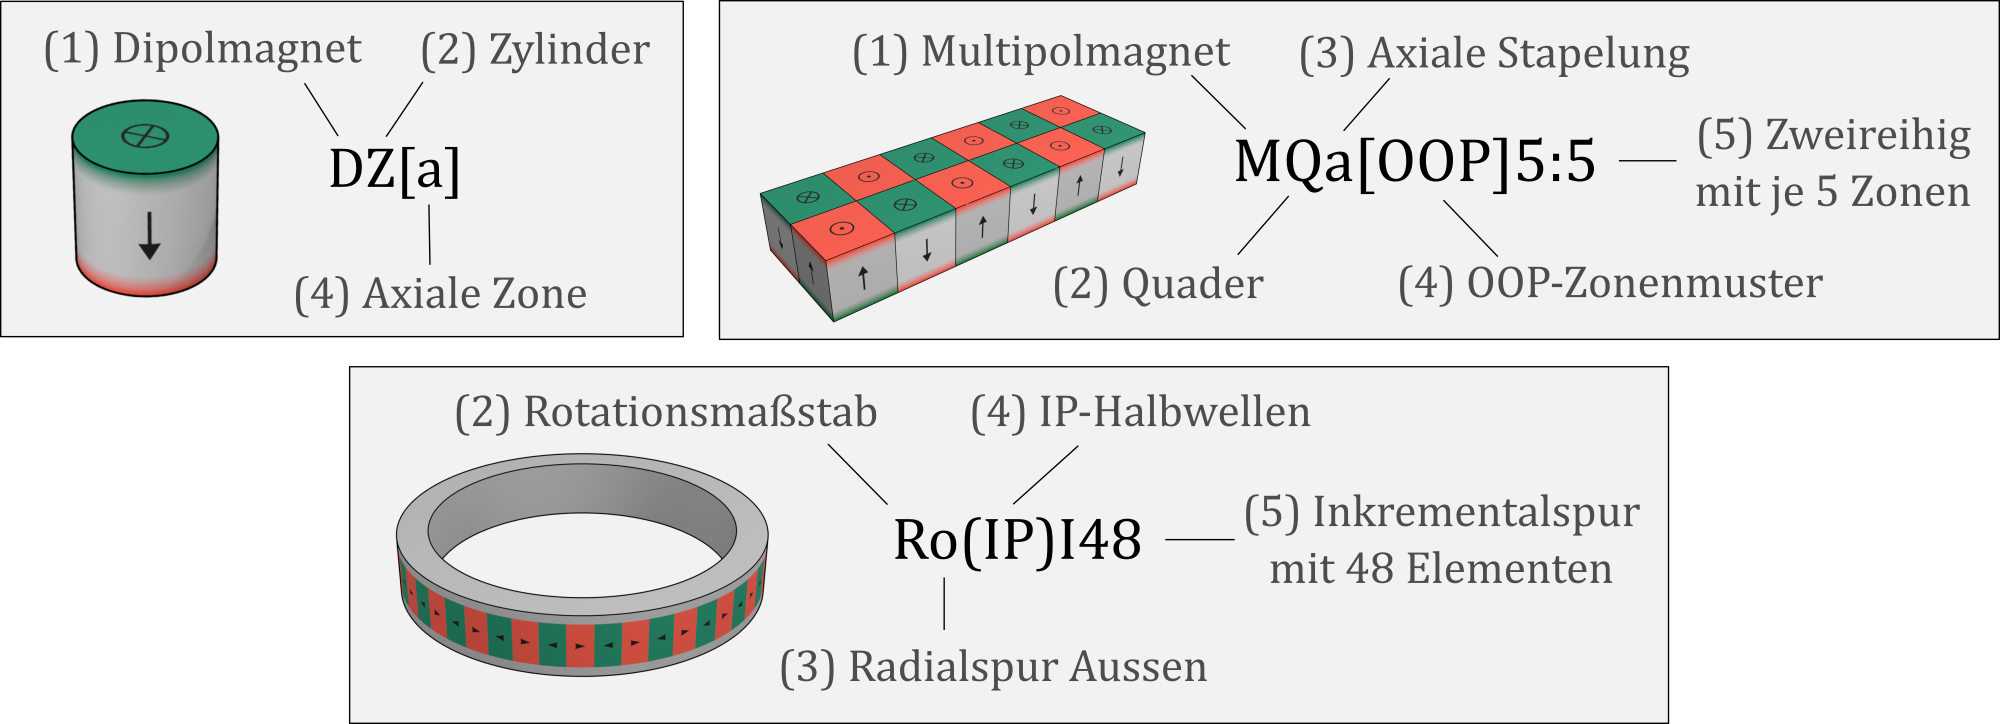
\includegraphics[width=0.85\linewidth,height=\textheight,keepaspectratio]{figures/sec07/01-kurznotation.png}

}

\caption{\label{fig-sec07-01-kurznotation}Kurznotation zur Einteilung}

\end{figure}%

Die Einteilung in fünf Ebenen bezieht sich auf die
\textbf{Repräsentation einer Maßverkörperung}. Insbesondere auf der
vierten Ebene kann dieselbe Maßverkörperung je nach Zweck zonenbezogen
über ein Zonenmuster oder feldbezogen über ein Polmuster beziehungsweise
die Ausprägung der Halbwellen beschrieben werden. Beispielsweise können
Ra{[}OOP{]}48 und Ra(iP)48 dieselbe Maßverkörperung einmal in
zonenbezogener und einmal in feldbezogener Repräsentation bezeichnen.

Das Einteilungssystem ist in der \textbf{Taxonomie magnetischer
Maßverkörperungen} in Abbildung~\ref{fig-sec07-14-taxonomie}
übersichtlich dargestellt. Die folgenden Unterkapitel beschreiben die
Einteilungsebenen für jede der drei Hauptgruppen im Detail.

\section{Dipolmagnete}\label{sec-07-dipolmagnete}

\textbf{Dipolmagnete} (D) sind magnetische Maßverkörperungen, deren
Polarisation durch eine einzelne magnetisierte Zone beschrieben werden
kann. Im Außenraum wird das Magnetfeld typischerweise durch den
Dipolanteil dominiert. Sie stellen damit hinsichtlich ihrer magnetischen
Struktur die einfachste Art dar.

Auf der \textbf{zweiten Einteilungsebene} werden Dipolmagnete anhand
ihrer geometrischen \textbf{Form} unterschieden. Die gängigste
Ausführung ist der Quader (Q). Abhängig vom Verhältnis seiner
Kantenlängen werden quaderförmige Magnete häufig auch als Würfel-,
Platten- oder Stabmagnete bezeichnet. Weitere verbreitete Formen sind
Zylinder (Z), Ringe (R), Ringsegmente (S) und Trapezprismen (T).
Trapezprismen werden insbesondere als Einzelmagnete zum Aufbau
zusammengesetzter magnetischer Strukturen, beispielsweise von
Halbach-Anordnungen, eingesetzt.

Die \textbf{dritte} und die \textbf{fünfte Einteilungsebene} entfallen
bei Dipolmagneten, da sie nur aus einer einzelnen Zone bestehen.

Die magnetische Ausprägung auf der \textbf{vierten Einteilungsebene}
wird durch die \textbf{Polarisationsrichtung} beschrieben. Quaderförmige
Dipolmagnete sind typischerweise entlang einer ihrer Hauptachsen
polarisiert. Bei Zylindern und Ringen werden insbesondere axiale (a),
diametrale (d) und radiale (r) Polarisation unterschieden. Axiale
Polarisation verläuft parallel zur Zylinderachse, diametrale
Polarisation senkrecht dazu und radiale Polarisation in radialer
Richtung. Freie Polarisationsrichtungen (f) werden angegeben, wenn die
Polarisation keiner der definierten Standardrichtungen entspricht.

Abbildung~\ref{fig-sec07-02-dipolmagnete} zeigt typische Beispiele der
hier beschriebenen Ausführungen in farbcodierter Zonendarstellung.

\begin{figure}[h]

\centering{

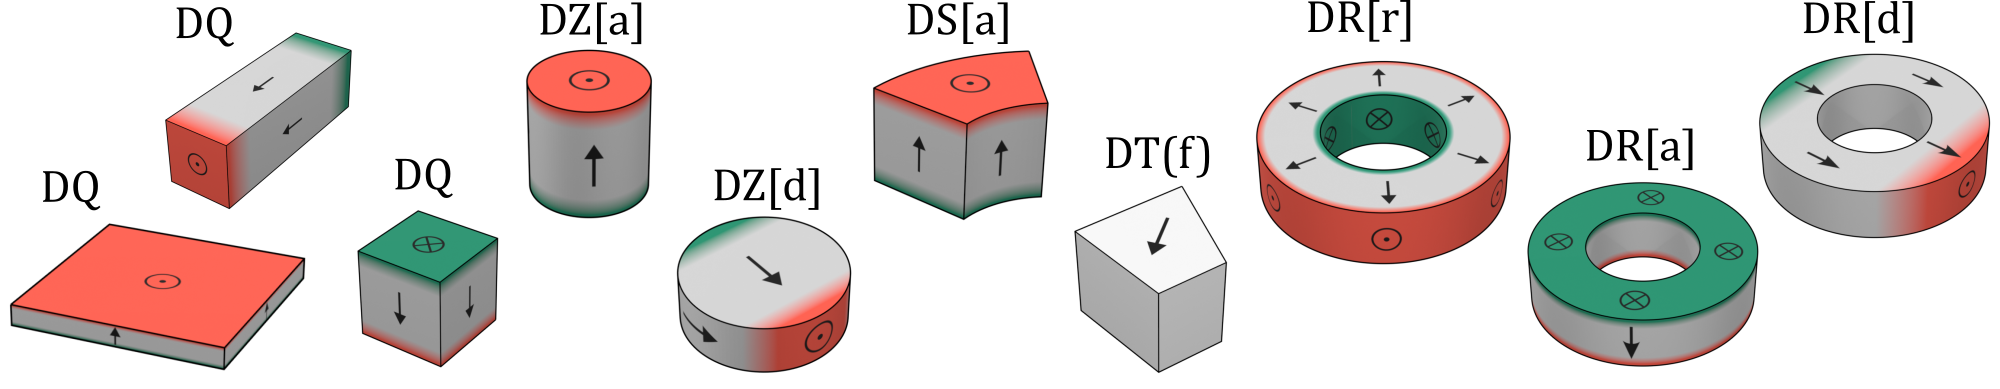
\includegraphics[width=1\linewidth,height=\textheight,keepaspectratio]{figures/sec07/02-dipolmagnete.png}

}

\caption{\label{fig-sec07-02-dipolmagnete}Beispielhafte Dipolmagnete}

\end{figure}%

\section{Multipolmagnete}\label{sec-07-multipolmagnete}

\textbf{Multipolmagnete} (M) sind magnetische Maßverkörperungen, die aus
mehreren Zonen bestehen. Im Unterschied zu magnetischen Maßstäben ist
ihre magnetische Struktur weniger komplex und nicht in magnetische
Spuren gegliedert.

Auf der \textbf{zweiten Einteilungsebene} wird ihre geometrische
\textbf{Form} beschrieben. Analog zu Dipolmagneten werden insbesondere
Quader (Q), Zylinder (Z), Ringe (R) und Ringsegmente (S) unterschieden.
Entspricht die Form der Maßverkörperung wegen komplexer Zusammensetzung
keiner der hier beschriebenen Formen, kann man sich auch auf die
Zonenform beziehen, siehe MTs{[}h{]}8 in
Abbildung~\ref{fig-sec07-03-multipolmagnete}.

Auf der \textbf{dritten Einteilungsebene} wird die geometrische
\textbf{Anordnung} der Zonen beschrieben. Die Zonen können geradlinig
beziehungsweise axial (a) oder sektoral beziehungsweise kreisförmig (s)
gestapelt sein. Darüber hinaus wird zwischen einreihigen und
mehrreihigen Anordnungen unterschieden. Die Zonenform der
Maßverkörperung ergibt sich aus ihrer geometrischen Form und der
Stapelung.

Die \textbf{magnetische Ausprägung} von Multipolmagneten auf der
\textbf{vierten Einteilungsebene} ist typischerweise durch das
Zonenmuster oder das Polmuster gegeben. Bei quaderförmigen und sektoral
gestapelten Anordnungen wird zwischen out-of-plane (OOP), in-plane (IP)
und Halbach-Anordnungen (h) unterschieden. Bei rotationssymmetrischen
Formen werden analog zu Dipolmagneten axiale (a), diametrale (d) und
radiale (r) Polarisationsrichtungen unterschieden. Die Polarisation
benachbarter Zonen ist dabei alternierend ausgerichtet. Zonen- und
Polmuster, die keiner dieser Klassen zugeordnet werden können, werden
als frei (f) gekennzeichnet.

Auf der \textbf{fünften Einteilungsebene} wird die Struktur durch die
\textbf{Anzahl der Zonen} oder Pole weiter spezifiziert. Bei
mehrreihigen Anordnungen wird sie für jede Reihe getrennt angegeben.

Abbildung~\ref{fig-sec07-03-multipolmagnete} zeigt typische Beispiele
der hier beschriebenen Ausführungen.

\begin{figure}[h]

\centering{

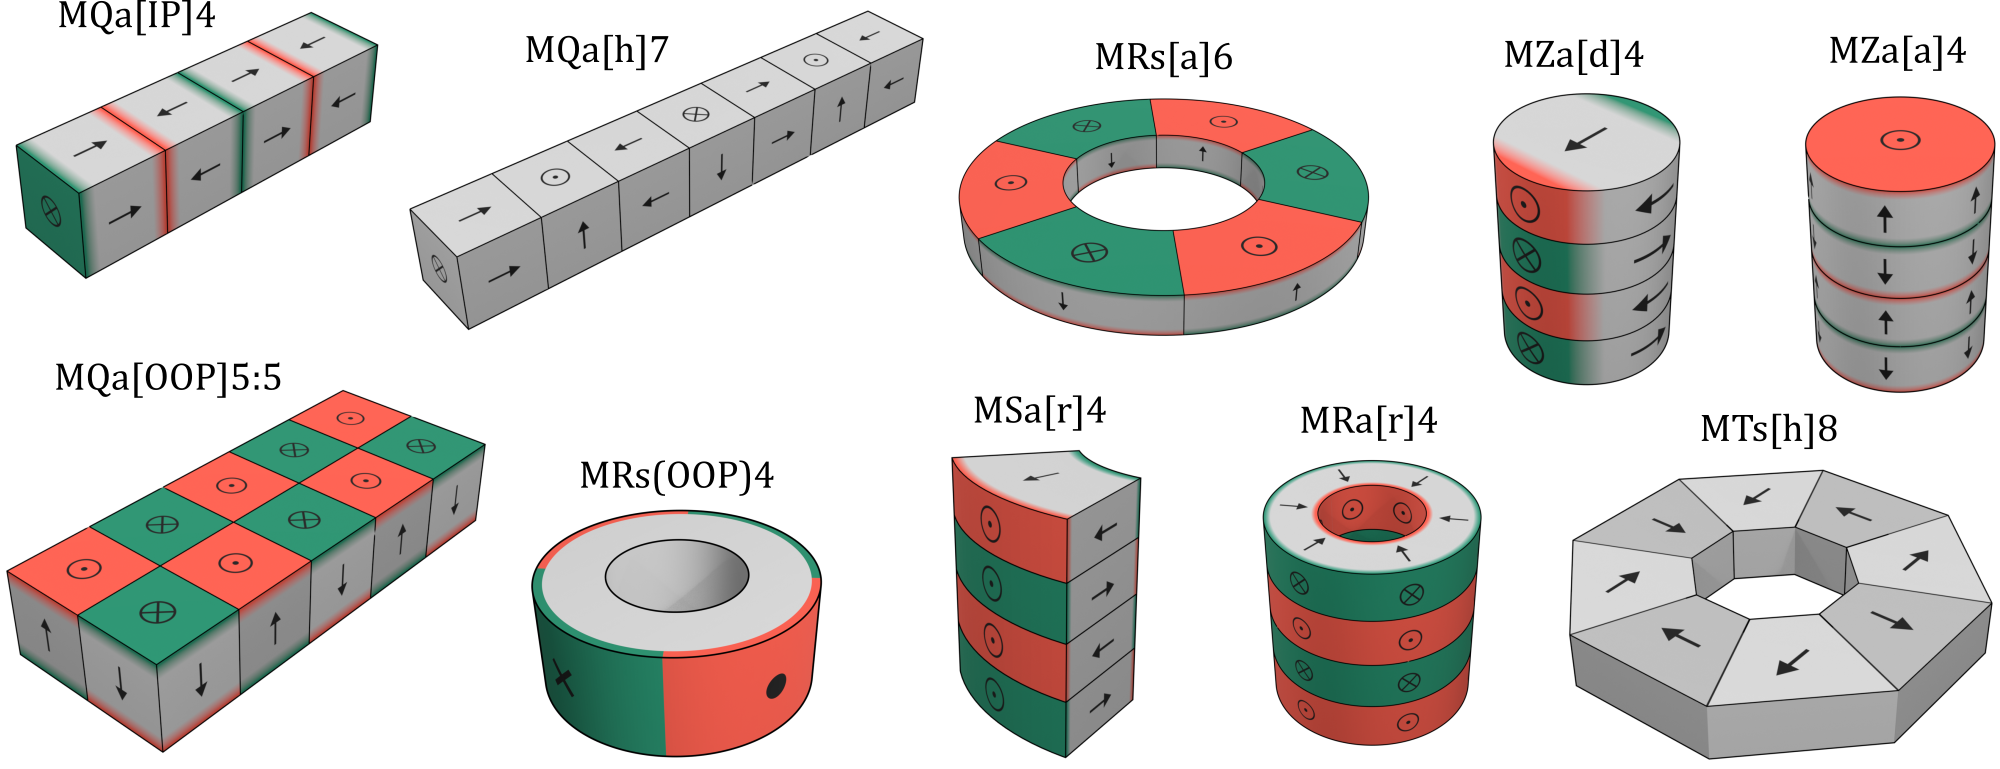
\includegraphics[width=1\linewidth,height=\textheight,keepaspectratio]{figures/sec07/03-multipolmagnete.png}

}

\caption{\label{fig-sec07-03-multipolmagnete}Beispielhafte
Multipolmagnete}

\end{figure}%

\section{Magnetische Maßstäbe}\label{sec-07-massstaebe}

\textbf{Magnetische Maßstäbe} sind Maßverkörperungen mit komplexer
magnetischer Struktur, die in eine oder mehrere magnetische Spuren
gegliedert ist. Auf \textbf{zweiter Ebene} unterscheidet man
Linearmaßstäbe (L) und Rotationsmaßstäbe (R). Auf \textbf{dritter Ebene}
werden Rotationsmaßstäbe in Maßstäbe mit innenliegender Radialspuren
(i), außenliegender Radialspuren (o) und Axialspuren (a) eingeteilt.

Die Beschreibung der \textbf{magnetischen Ausprägung} auf der
\textbf{vierten Einteilungsebene} kann zonen- oder feldbezogen erfolgen.
Typische Zonenmuster sind in-plane (IP), out-of-plane (OOP) und
Halbach-Anordnungen (h). Feldbezogen erfolgt die Beschreibung über das
Polmuster oder über die Halbwellen einer ausgewählten Komponente des
Streufeldes. Dabei werden in-plane- (IP) und out-of-plane-Komponenten
(OOP) unterschieden.

Auf der \textbf{fünften Einteilungsebene} wird die magnetische Struktur
durch den \textbf{Spurtyp} sowie gegebenenfalls eine zugehörige
Kenngröße gekennzeichnet, die die \textbf{Anzahl} der Elemente oder
Referenzlagen angibt. Bei mehrspurigen Maßstäben werden die Angaben für
die einzelnen Spuren durch Doppelpunkte getrennt angegeben.

Die \textbf{Spurtypen} beschreiben die magnetische Strukturierung einer
Spur und dienen ihrer funktionalen Unterscheidung. Ein Spurtyp kann
durch unterschiedliche Zonenmuster, beispielsweise IP, OOP oder Halbach,
realisiert und sowohl zonen- als auch feldbezogen beschrieben werden. In
den nachfolgend dargestellten schematischen Mustern werden Zonen, Pole
und Halbwellen abstrahierend als Elemente bezeichnet; Richtungssymbole
werden nicht verwendet. Im Zweifelsfall beziehen sich die dargestellten
Elemente auf Halbwellen.

\textbf{Inkrementalspuren} (I\(x\)) bestehen aus \(x\) alternierenden
Elementen gleicher Länge. Das daraus resultierende periodische Spurfeld
ermöglicht die Erfassung relativer Lage-, Winkel- oder
Geschwindigkeitsänderungen mit hoher Ortsauflösung. Ein Beispiel ist in
Abbildung~\ref{fig-sec07-04-inkremental} gezeigt.

\begin{figure}[H]

\centering{


\includegraphics[width=0.7\linewidth,height=\textheight,keepaspectratio]{figures/sec07/04-inkremental.png}

}

\caption{\label{fig-sec07-04-inkremental}Spurtypen -- Inkrementalspur
I24}

\end{figure}%

\textbf{Referenzspuren} (R\(x\)) kennzeichnen \(x\) definierte
Referenzlagen, beispielsweise Start- oder Endlagen. Eine Referenz wird
typischerweise nicht durch ein einzelnes Element, sondern durch eine
charakteristische Kombination mehrerer Elemente gebildet. Ein Beispiel
ist in Abbildung~\ref{fig-sec07-05-referenz} gezeigt.

\begin{figure}[H]

\centering{


\includegraphics[width=0.7\linewidth,height=\textheight,keepaspectratio]{figures/sec07/05-referenz.png}

}

\caption{\label{fig-sec07-05-referenz}Spurtypen -- Referenzspur R1}

\end{figure}%

Eine Sonderform bilden \textbf{abstandscodierte Referenzspuren}
(RC\(x\)) mit \(x\) Referenzlagen. Die Lage wird dabei aus dem Abstand
zwischen aufeinanderfolgenden Referenzen bestimmt. Ein Beispiel ist in
Abbildung~\ref{fig-sec07-06-referenz2} gezeigt.

\begin{figure}[H]

\centering{


\includegraphics[width=0.7\linewidth,height=\textheight,keepaspectratio]{figures/sec07/06-referenz2.png}

}

\caption{\label{fig-sec07-06-referenz2}Spurtypen -- Abstandscodierte
Referenzspur RC3}

\end{figure}%

Für bestimmte Anwendungen können Spuren mit variablen Elementlängen
eingesetzt werden. Ein wichtiger Vertreter ist der
\textbf{Pseudorandomcode} (P), auch als pseudo-random binary sequence
bezeichnet. Dabei handelt es sich um eine Codierung, aus der mit
geeigneter Sensorik die absolute Lage bestimmt werden kann. Ein Beispiel
ist in Abbildung~\ref{fig-sec07-07-pseudorandom} gezeigt.

\begin{figure}[H]

\centering{


\includegraphics[width=0.7\linewidth,height=\textheight,keepaspectratio]{figures/sec07/07-pseudorandom.png}

}

\caption{\label{fig-sec07-07-pseudorandom}Spurtypen -- Pseudorandomcode
P}

\end{figure}%

Die Bestimmung der Absolutlage ist auch mit \textbf{gedrehten
Elementgrenzen} (V) möglich. Ein Beispiel ist in
Abbildung~\ref{fig-sec07-08-gedreht} gezeigt.

\begin{figure}[H]

\centering{


\includegraphics[width=0.7\linewidth,height=\textheight,keepaspectratio]{figures/sec07/08-gedreht.png}

}

\caption{\label{fig-sec07-08-gedreht}Spurtypen -- Gedrehte Grenzen V}

\end{figure}%

\textbf{Kombinationen mehrerer parallel verlaufender Spuren} eröffnen
weitere Anwendungsmöglichkeiten. Beispielsweise kann eine
Inkrementalspur mit einer Referenzspur kombiniert werden, um einen
definierten Bezugspunkt für die Zählung der Inkremente festzulegen. Nach
dem Anfahren der Referenzlage kann daraus eine absolute Lage mit der
hohen Genauigkeit der Inkrementalspur bestimmt werden. Ein Beispiel ist
in Abbildung~\ref{fig-sec07-09-incremental-referenz} gezeigt.

\begin{figure}[H]

\centering{

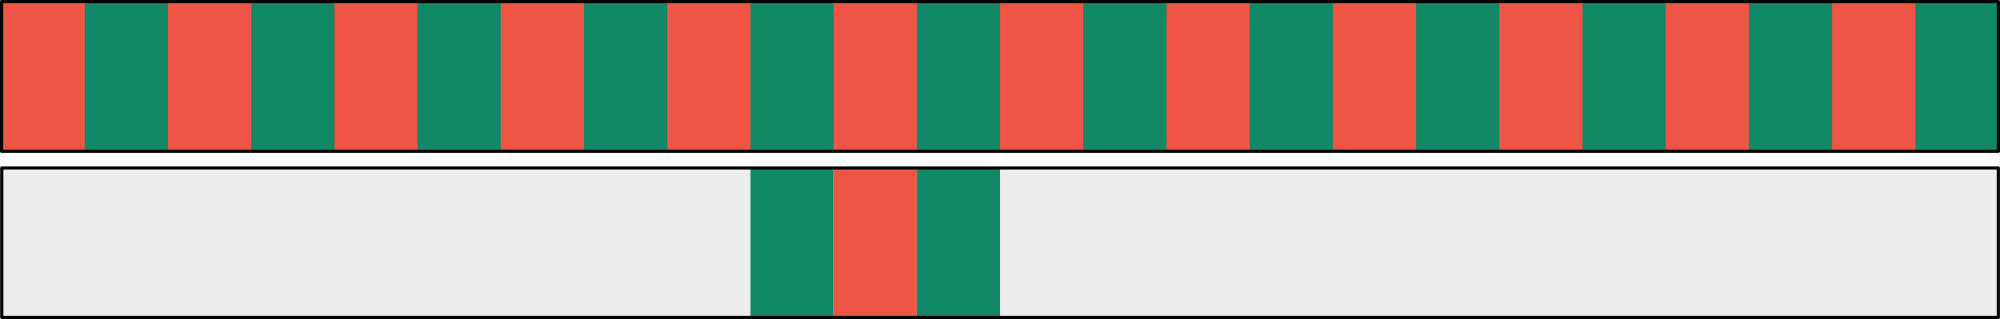
\includegraphics[width=0.7\linewidth,height=\textheight,keepaspectratio]{figures/sec07/09-incremental-referenz.png}

}

\caption{\label{fig-sec07-09-incremental-referenz}Spurtypen --
Inkrementalspur mit Referenzspur I24:R1}

\end{figure}%

Auch bei der Kombination einer Inkrementalspur mit einer
abstandscodierten Referenzspur kann eine absolute Lage bestimmt werden.
Dies ist gegenüber der Kombination mit einfacher Referenzspur bereits
nach kürzerer Relativbewegung möglich. Ein entsprechendes Beispiel ist
in Abbildung~\ref{fig-sec07-10-inkremental-referenz2} gezeigt.

\begin{figure}[H]

\centering{

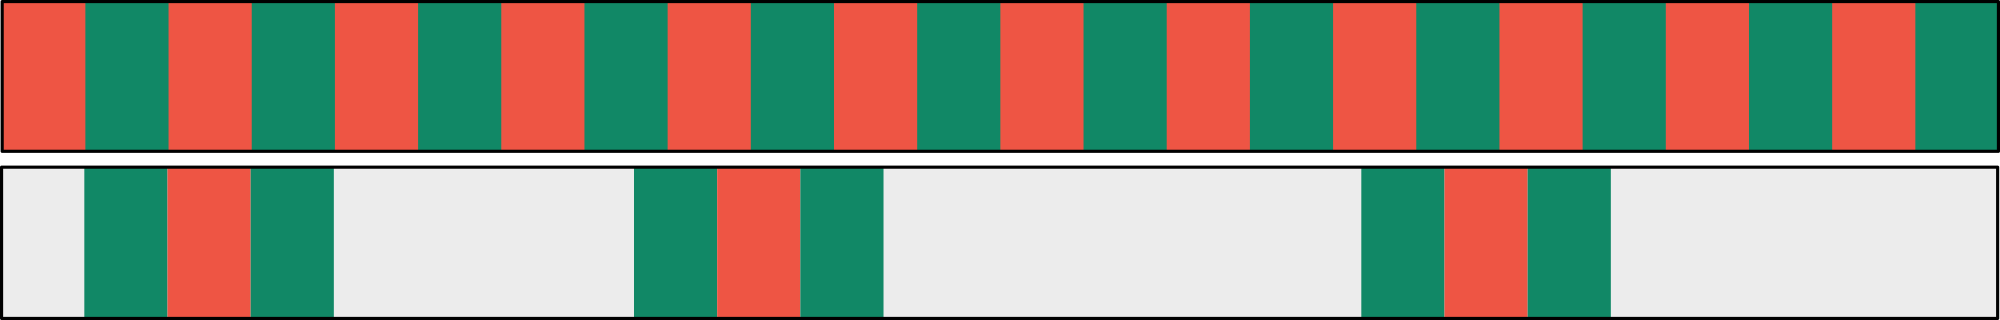
\includegraphics[width=0.7\linewidth,height=\textheight,keepaspectratio]{figures/sec07/10-inkremental-referenz2.png}

}

\caption{\label{fig-sec07-10-inkremental-referenz2}Spurtypen --
Inkrementalspur mit abstandscodierter Referenzspur I24:RC}

\end{figure}%

Wenn zwei Inkrementalspuren nebeneinander angeordnet sind und sich ihre
Elementanzahlen in einem definierten Verhältnis unterscheiden, kann aus
dem Phasenbezug zwischen den beiden Spuren die Absolutlage bestimmt
werden. Die Kombination wird häufig als \textbf{Noniusmuster}
bezeichnet. Ein Beispiel ist in Abbildung~\ref{fig-sec07-11-nonius}
gezeigt.

\begin{figure}[H]

\centering{

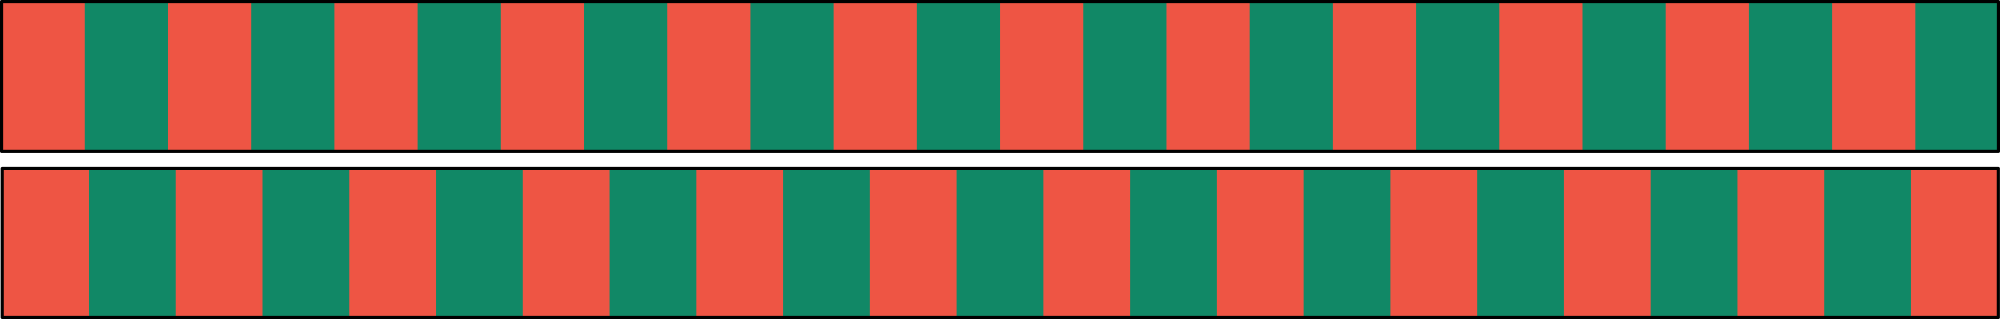
\includegraphics[width=0.7\linewidth,height=\textheight,keepaspectratio]{figures/sec07/11-nonius.png}

}

\caption{\label{fig-sec07-11-nonius}Spurtypen -- Noniusmuster I23:I24}

\end{figure}%

Mit einem Pseudorandomcode kann die absolute Lage direkt bestimmt
werden. Die erreichbare Auflösung ist jedoch begrenzt. Durch die
Kombination mit einer Inkrementalspur können Messauflösung und
-genauigkeit erhöht werden. Dabei liefert die Pseudorandomcode-Spur die
absolute Lage, während die Inkrementalspur zur höher aufgelösten
Feinbestimmung und gegebenenfalls zur Korrektur verwendet wird. Ein
Beispiel ist in Abbildung~\ref{fig-sec07-12-inkremental_pseudo} gezeigt.

\begin{figure}[H]

\centering{

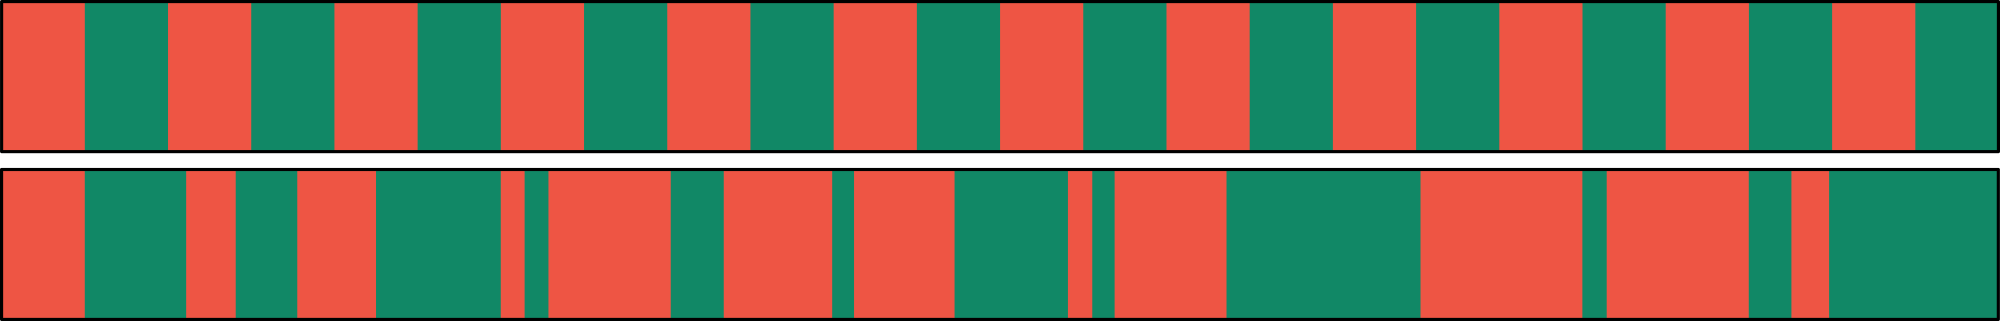
\includegraphics[width=0.7\linewidth,height=\textheight,keepaspectratio]{figures/sec07/12-inkremental-pseudo.png}

}

\caption{\label{fig-sec07-12-inkremental_pseudo}Spurtypen --
Inkrementalspur mit Pseudorandomcode I24:P}

\end{figure}%

Die nachfolgende Abbildung~\ref{fig-sec07-13-massstabe} zeigt Beispiele
typischer magnetischer Maßstäbe mit der jeweils zugehörigen
Kurznotation.

\begin{figure}[h]

\centering{

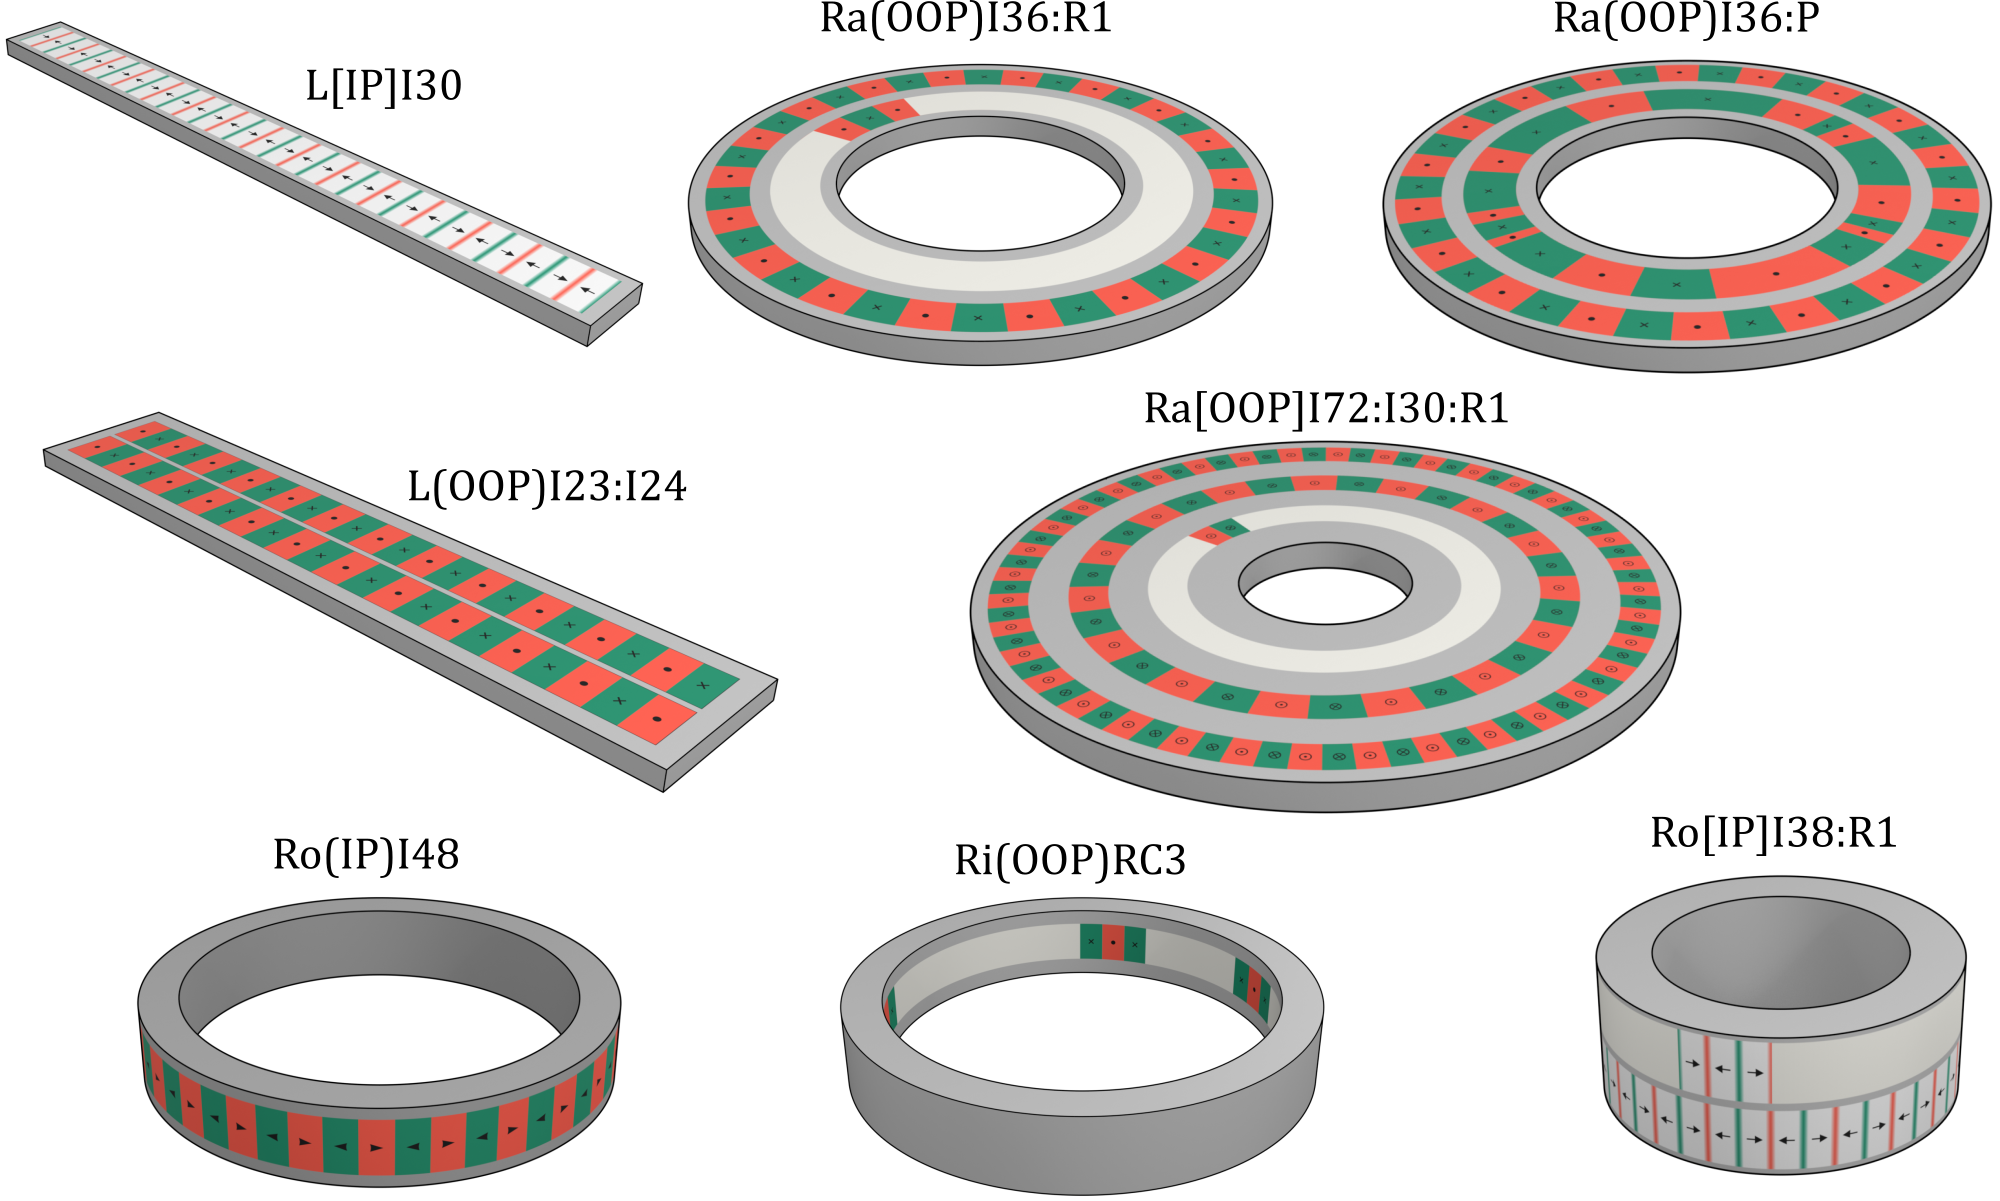
\includegraphics[width=1\linewidth,height=\textheight,keepaspectratio]{figures/sec07/13-massstabe.png}

}

\caption{\label{fig-sec07-13-massstabe}Beispielhafte magnetische
Maßstäbe}

\end{figure}%

\clearpage
\begin{landscape}

\section{Taxonomie magnetischer
Maßverkörperungen}\label{sec-07-taxonomie}

\begin{figure}[H]

\centering{

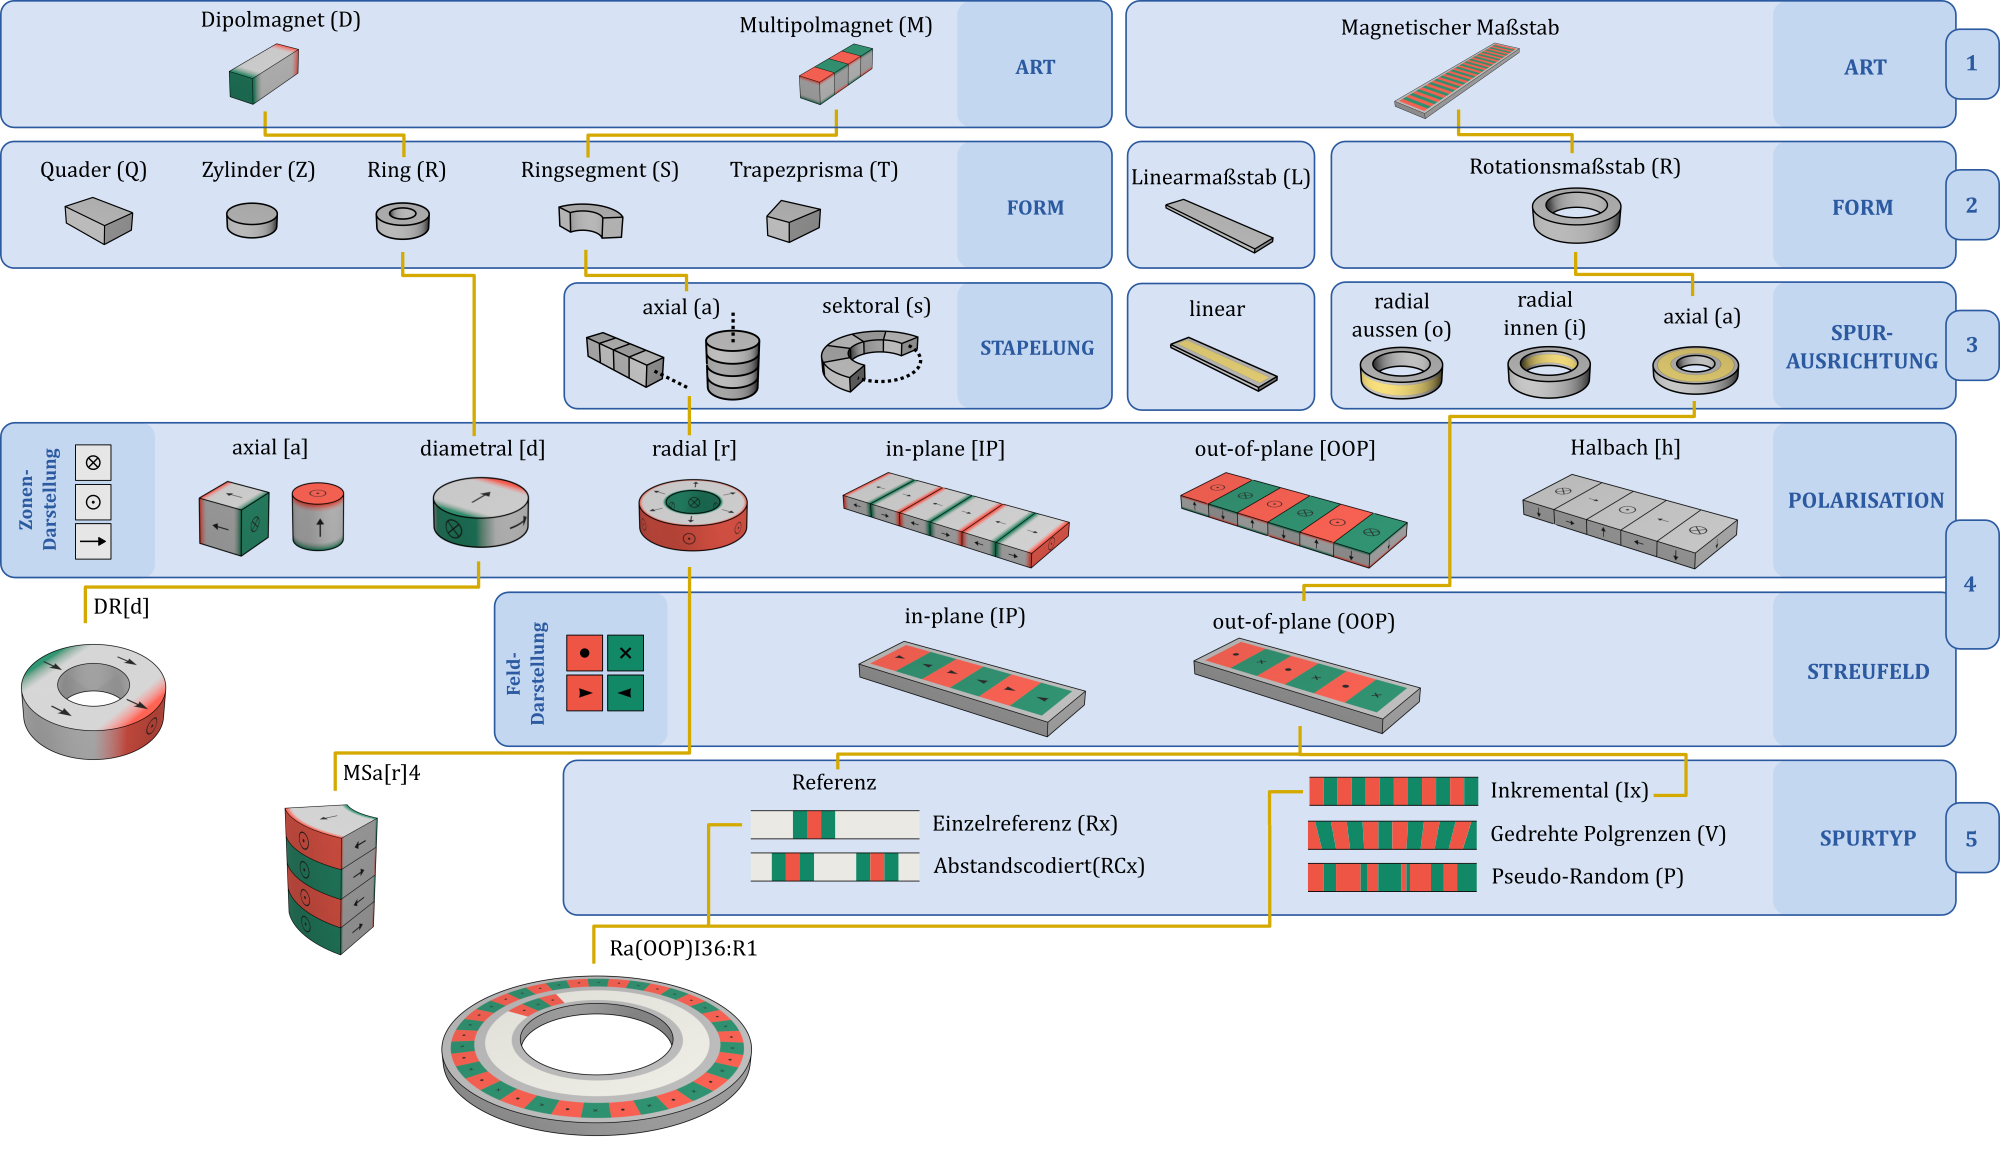
\includegraphics[width=1\linewidth,height=\textheight,keepaspectratio]{figures/sec07/14-taxonomie.png}

}

\caption{\label{fig-sec07-14-taxonomie}Taxonomie magnetischer
Maßverkörperungen}

\end{figure}%

\end{landscape}
\clearpage

\bookmarksetup{startatroot}

\chapter{Schnittstelle zur Sensorik}\label{sec-08}

Der Sensor erfasst das von der Maßverkörperung erzeugte Streufeld und
bildet damit die Schnittstelle zwischen Maßverkörperung und Messsystem.
Seine konkrete technologische Ausführung ist nicht Gegenstand dieser
Richtlinie. Im Folgenden werden jedoch die für die Beschreibung
magnetischer Messsysteme erforderlichen sensorbezogenen Begriffe zum
Aufbau des Sensormoduls, zur Erfassung des Streufeldes sowie zur
Lagebeziehung zwischen Sensor und Maßverkörperung eingeführt.

\section{Sensorart und -funktion}\label{sec-08-sensorart_funktion}

Magnetische Sensoren können nach der \textbf{Art der ausgegebenen
Messgröße} unterschieden werden. Ein \textbf{Magnetfeldsensor} dient
dazu, den Wert einer oder mehrerer Komponenten des Magnetfeldvektors
ortsbezogen zu erfassen und als feldbezogene Ausgangsgröße
bereitzustellen. Ein \textbf{magnetischer Positions- oder Winkelsensor}
erfasst ebenfalls das Magnetfeld, verarbeitet dieses jedoch intern
weiter und gibt als Ausgangsgröße unmittelbar eine Positions- oder
Winkelinformation aus. Während der Magnetfeldsensor somit eine
feldbezogene Messgröße liefert, stellt der magnetische Positions- oder
Winkelsensor bereits eine anwendungsbezogene Ausgangsgröße bereit.

Unabhängig von der Art der Ausgangsgröße können Sensoren nach ihrer
\textbf{Funktion} im jeweiligen Anwendungs- oder Prüfkontext
unterschieden werden. Ein \textbf{Prüfsensor} bezeichnet dabei keine
eigene Sensorart, sondern die Funktion eines Sensors, der zu Prüf-,
Einstell- oder Charakterisierungszwecken eingesetzt wird; hierbei
handelt es sich in der Regel um einen Magnetfeldsensor. Ein
\textbf{Referenzsensor} dient der Bereitstellung eines Vergleichs- oder
Bezugswertes. Ein \textbf{Betriebssensor} ist der im regulären Betrieb
des Systems eingesetzte Sensor, dessen Ausgangssignal für die
vorgesehene Funktion des Systems genutzt wird.

\section{Aufbau des Sensormoduls}\label{sec-08-aufbau_sensormodul}

Ein \textbf{Sensormodul} ist eine funktionale Einheit zur Erfassung und
Verarbeitung magnetischer Messgrößen. Es umfasst ein oder mehrere
magnetisch sensitive Sensorelemente sowie gegebenenfalls weitere
Komponenten für Versorgung, Signalaufbereitung, Datenverarbeitung und
elektrische Anbindung.

Das \textbf{Sensorelement} bezeichnet das eigentliche Wandlerelement,
das eine magnetische Messgröße erfasst und in eine elektrische Größe
umwandelt. In einem Sensormodul können mehrere Sensorelemente räumlich
unterschiedlich angeordnet sein und unterschiedliche Komponenten des
Magnetfeldes erfassen.

Bei Sensoren in Halbleitertechnik sind ein oder mehrere Sensorelemente
typischerweise auf einem \textbf{Sensorchip} integriert. Der Sensorchip
kann zusammen mit elektrischen Kontaktierungen und weiteren Bauelementen
in einem \textbf{Package} zusammengefasst sein. Das Package schützt den
Chip und stellt insbesondere die mechanische und elektrische
Schnittstelle zur weiteren Integration bereit.

Ein Package kann unmittelbar das äußere \textbf{Sensorgehäuse} bilden
oder zusammen mit weiteren Komponenten in ein separates Sensorgehäuse
integriert sein. Das vollständige Sensormodul kann darüber hinaus
beispielsweise eine \textbf{Leiterplatte}, zusätzliche elektronische
Bauelemente, Steckverbinder und mechanische Befestigungselemente
umfassen.

Die genannten Integrationsebenen sind nicht bei allen Sensoren getrennt
ausgeführt und stellen keine zwingende Aufbauhierarchie dar. Die
Begriffe dienen der eindeutigen Bezeichnung der jeweils betrachteten
funktionalen beziehungsweise konstruktiven Ebene.

\begin{figure}[h]

\centering{

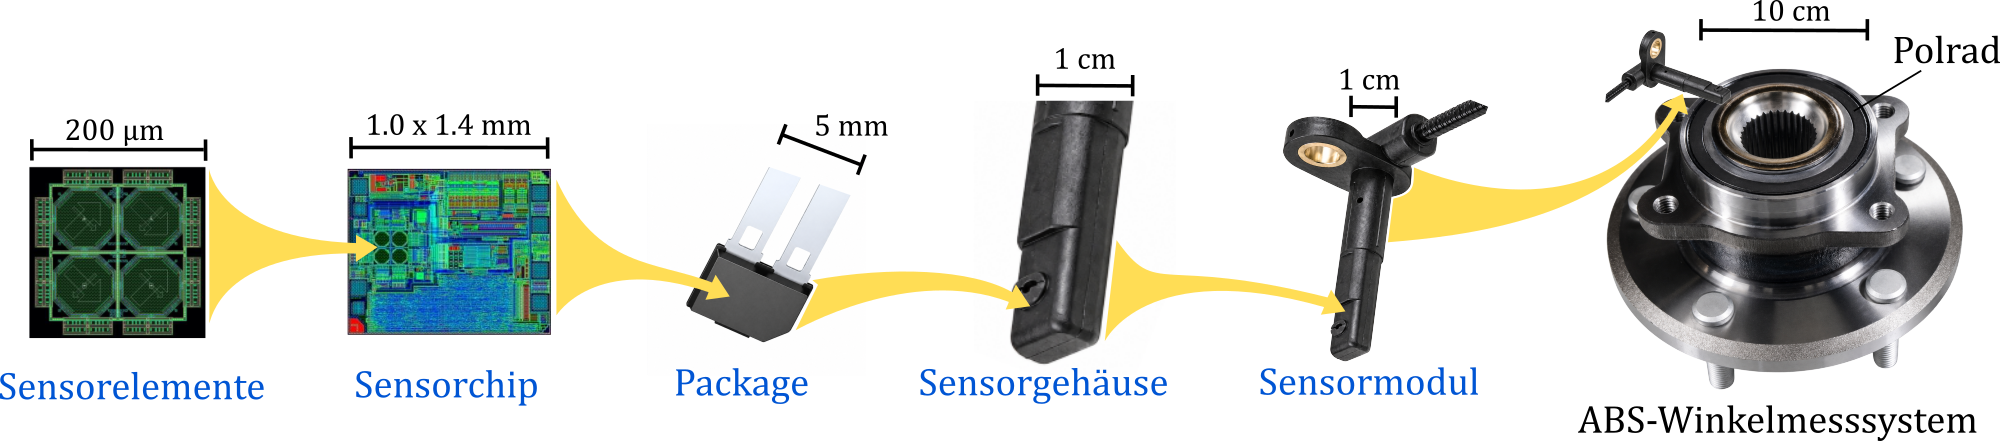
\includegraphics[width=1\linewidth,height=\textheight,keepaspectratio]{figures/sec08/01-sensormodul_aufbau.png}

}

\caption[\label{fig-sec08-01-sensormodul_aufbau}Beispielhafter Aufbau
eines Sensormoduls]{\label{fig-sec08-01-sensormodul_aufbau}Beispielhafter Aufbau
eines Sensormoduls\footnotemark{}}

\end{figure}%
\footnotetext{Quelle der Abbildungen: Infineon AG,
  Augustin Group GmbH und mit freundlicher Genehmigung von U.
  Ausserlechner; redaktionelle Aufbereitung durch Autoren.}

Abbildung~\ref{fig-sec08-01-sensormodul_aufbau} zeigt beispielhaft den
Aufbau eines Sensormoduls in Halbleitertechnik und veranschaulicht die
Integrationsebenen vom Sensorelement über Sensorchip, Package und
Sensorgehäuse bis zum Sensormodul.

\section{Lagebeziehung des Sensors}\label{sec-08-lagebeziehung-sensor}

Die in Kapitel~\ref{sec-05-ermittlungsbereich_und_feldverläufe}
eingeführten Ermittlungsbereiche beschreiben die räumlichen Bereiche, in
denen das Streufeld betrachtet beziehungsweise vermessen wird. In einem
realen Messaufbau werden sie durch eine entsprechende Lagebeziehung
zwischen Sensor und Maßverkörperung realisiert. In diesem Unterkapitel
wird die hierfür erforderliche Terminologie eingeführt.

Als \textbf{Sensorreferenz} \(O_S\) wird ein zweckmäßiger Bezugspunkt
für die Sensorelemente festgelegt. Er sollte die Lage der Sensorelemente
möglichst repräsentativ beschreiben, beispielsweise in der geometrischen
Mitte der Sensorelemente beziehungsweise des von ihnen eingenommenen
sensitiven Bereichs. Mit der Sensorreferenz als Ursprung wird ein
rechtshändiges \textbf{Sensor-KS} mit den Koordinatenrichtungen \(x\),
\(y\) und \(z\) definiert.

In diesem Bezugssystem werden Lage und geometrische Ausdehnung der
Sensorelemente beschrieben. Das ermöglicht eine einheitliche
geometrische Beschreibung der Sensorelemente, deren Ausführung stark von
der eingesetzten Sensortechnologie abhängen kann.

Bei \textbf{nominaler Ausrichtung} des Sensors verlaufen die \(x\)-,
\(y\)- und \(z\)-Richtung parallel zur lokalen \(p\)-, \(o\)-
beziehungsweise \(n\)-Richtung des Maßverkörperungs-KS.

Die \textbf{Sensorlage} \(\vec{r}_S\) bezeichnet die Lage der
Sensorreferenz im Maßverkörperungs-KS. Sie wird durch die Koordinaten
\(p_S\), \(o_S\) und \(n_S\) beschrieben. Durch die Relativbewegung von
Sensor und Maßverkörperung werden unter Berücksichtigung von Lage und
geometrischer Ausdehnung der Sensorelemente die entsprechenden
Ermittlungsbereiche erfasst.

Zur Beschreibung des \textbf{Abstands zwischen Sensor und
Maßverkörperung} wird aufgrund des oft mehrschichtigen Aufbaus von
Sensormodul und Maßverkörperung zwischen Luftspalt, Wirkabstand und
Messhöhe unterschieden.

Der \textbf{Luftspalt} \(d_\mathrm{mech}\) bezeichnet den freien
mechanischen Abstand zwischen den einander zugewandten Oberflächen von
Maßverkörperung und Sensorgehäuse. Er beschreibt damit eine konstruktive
Größe des Messsystems.

Der \textbf{Wirkabstand} \(d_\mathrm{mag}\) bezeichnet den Abstand in
lokaler \(n\)-Richtung zwischen der sensorzugewandten Begrenzung der
Zonenstruktur und der Sensorreferenz. Im Gegensatz zum Luftspalt
beschreibt er die Distanz zwischen der Oberseite der magnetisch
wirksamen Struktur und den Sensorelementen, unabhängig von
dazwischenliegenden magnetisch inaktiven Elementen wie Schutzabdeckungen
und Packages.

Die \textbf{Messhöhe} \(n\) bezeichnet die \(n\)-Koordinate im
Maßverkörperungs-KS und damit den Abstand von der funktionalen
Oberfläche. Die Messhöhe der Sensorreferenz entspricht dem Wirkabstand,

wenn die Begrenzung der Zonenstruktur mit der funktionalen Oberfläche
zusammenfällt, was beispielsweise bei Maßverkörperungen mit
Schutzabdeckungen nicht gegeben ist.

Die \textbf{Sensororientierung} bezeichnet die Orientierung des
Sensor-KS relativ zum lokalen Maßverkörperungs-KS an der Sensorlage. Bei
nominaler Ausrichtung stimmen die entsprechenden Koordinatenrichtungen
beider Koordinatensysteme überein.

Abweichungen von der nominalen Ausrichtung werden durch die
\textbf{Sensordrehwinkel} \(\alpha\) (Rotation um \(\vec{e}_p\)),
\(\beta\) (Rotation um \(\vec{e}_o\)) und \(\gamma\) (Rotation um
\(\vec{e}_n\)) beschrieben. Drehungen mit \(\alpha\) und \(\beta\)
führen zu einer Verkippung des Sensors gegenüber der funktionalen
Oberfläche, während eine Drehung mit \(\gamma\) einer Verdrehung
innerhalb der zur funktionalen Oberfläche parallelen Ebene entspricht.
Treten mehrere endliche Sensordrehwinkel gleichzeitig auf, ist die
verwendete Reihenfolge der Drehungen anzugeben.

\begin{figure}[h]

\centering{

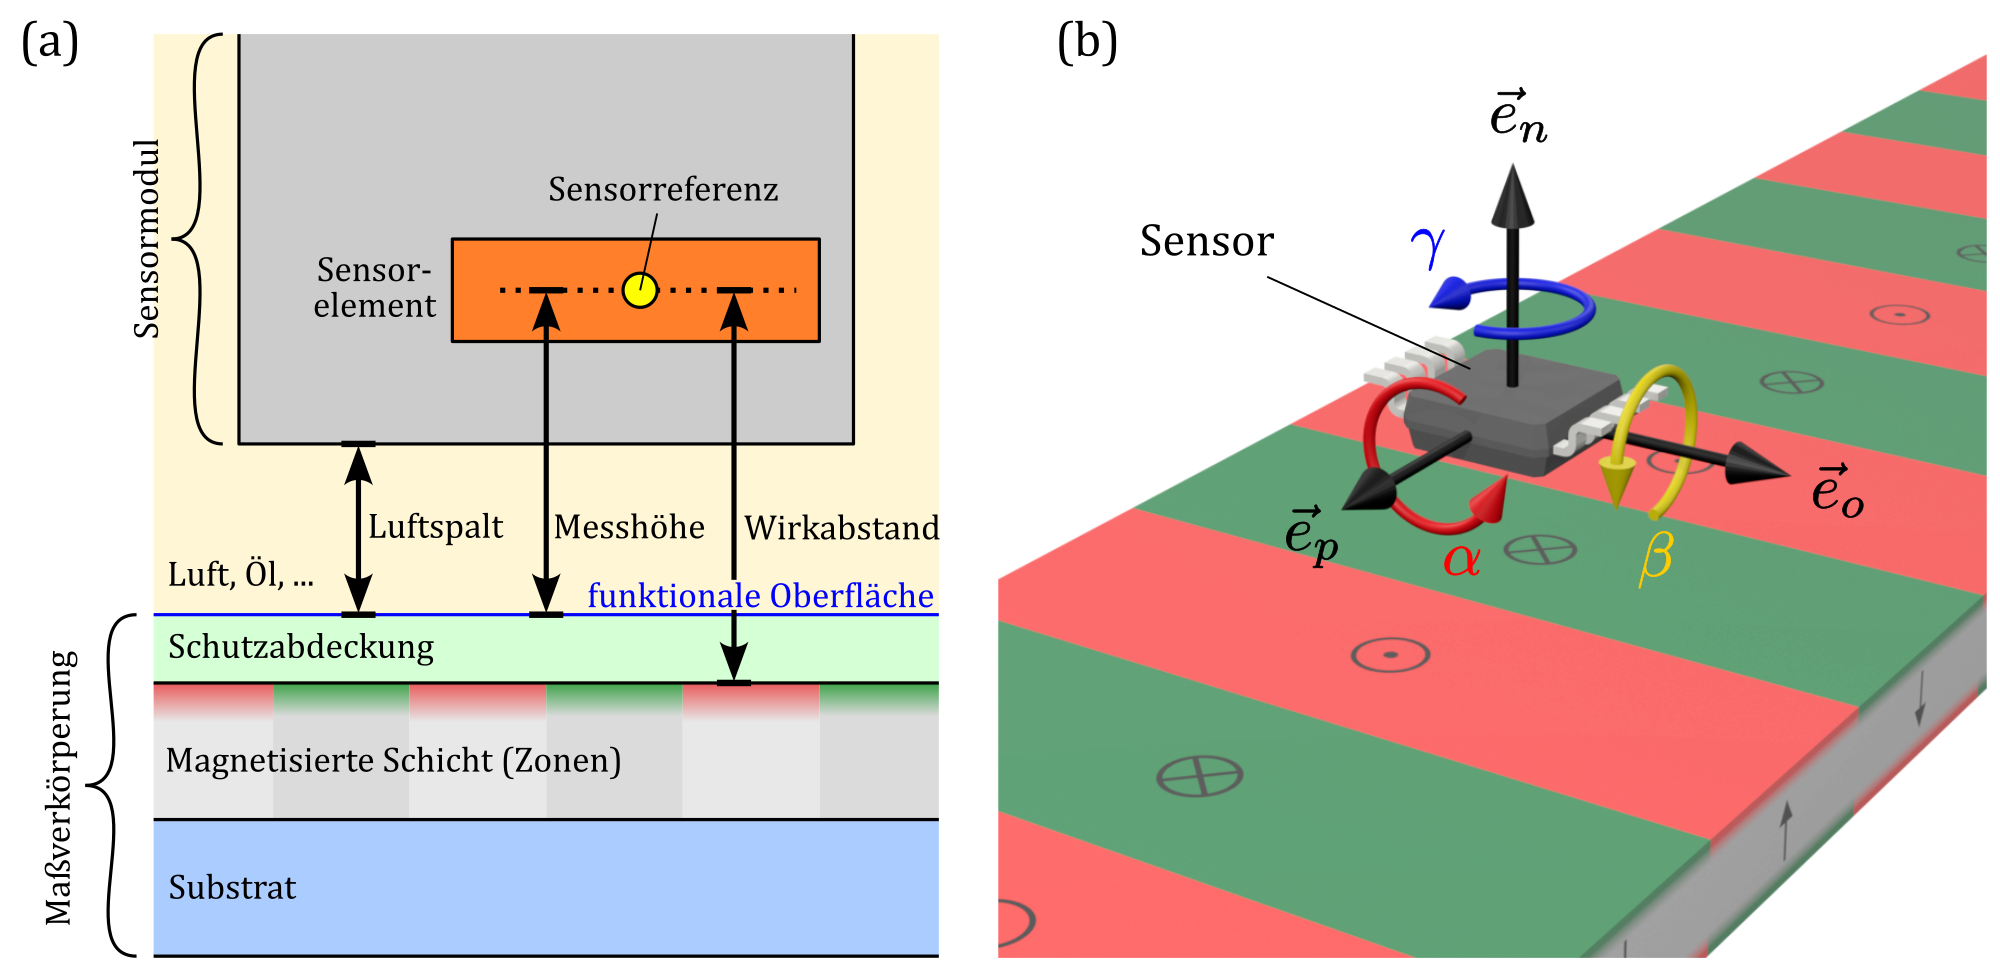
\includegraphics[width=1\linewidth,height=\textheight,keepaspectratio]{figures/sec08/02-sensor_lage.png}

}

\caption{\label{fig-sec08-02-sensor_lage}Lagebeziehung des Sensors}

\end{figure}%

Abbildung~\ref{fig-sec08-02-sensor_lage} veranschaulicht die
Lagebeziehung zwischen Sensor und Maßverkörperung. Teilbild (a) zeigt
die Größen Luftspalt, Wirkabstand und auf die Sensorreferenz bezogene
Messhöhe. Teilbild (b) zeigt die Sensordrehwinkel.

\begingroup
\footnotesize
\renewcommand{\baselinestretch}{1.12}\selectfont
\setlength{\tabcolsep}{5pt}
\setlength{\extrarowheight}{2.5pt}
\renewcommand{\arraystretch}{1.15}
{\begin{longtable}[]{
  >{\raggedright\arraybackslash}p{(\linewidth - 4\tabcolsep) * \real{0.2500}}
  >{\centering\arraybackslash}p{(\linewidth - 4\tabcolsep) * \real{0.1500}}
  >{\raggedright\arraybackslash}p{(\linewidth - 4\tabcolsep) * \real{0.6000}}}
\caption{Begriffe Sensorlage}\label{tbl-begriffe-sensorlage}\tabularnewline
\arrayrulecolor{tableouterrule}
\toprule\noalign{}
\rowcolor{zebrabluehead}
\begin{minipage}[b]{\linewidth}\raggedright
\textbf{Begriff}
\end{minipage} & \begin{minipage}[b]{\linewidth}\centering
\textbf{Symbol}
\end{minipage} & \begin{minipage}[b]{\linewidth}\raggedright
\textbf{Beschreibung}
\end{minipage} \\
\arrayrulecolor{tableheadrule}
\specialrule{0.35pt}{0pt}{0pt}
\endhead
\arrayrulecolor{tableouterrule}
\specialrule{0.30pt}{0pt}{0pt}
\endlastfoot
\rowcolor{zebrabluelight}
\textbf{Sensorlage} & \(\vec{r}_S\) & Lage der Sensorreferenz im
Maßverkörperungs-KS \\
\arrayrulecolor{tableline}
\specialrule{0.15pt}{0pt}{0pt}
\rowcolor{zebrabluedark}
\textbf{Luftspalt} & \(d_\mathrm{mech}\) & Freier mechanischer Abstand
zwischen Sensorgehäuse und Maßverkörperung \\
\arrayrulecolor{tableline}
\specialrule{0.15pt}{0pt}{0pt}
\rowcolor{zebrabluelight}
\textbf{Wirkabstand} & \(d_\mathrm{mag}\) & Abstand zwischen der
Oberseite der Zonenstruktur und der Sensorreferenz \\
\arrayrulecolor{tableline}
\specialrule{0.15pt}{0pt}{0pt}
\rowcolor{zebrabluedark}
\textbf{Messhöhe} & \(n\) & \(n\)-Koordinate im Maßverkörperungs-KS;
Abstand von der funktionalen Oberfläche \\
\arrayrulecolor{tableline}
\specialrule{0.15pt}{0pt}{0pt}
\rowcolor{zebrabluelight}
\textbf{Sensordrehwinkel} & \(\alpha, \beta, \gamma\) & Drehwinkel zur
Beschreibung der Orientierung des Sensors gegenüber der nominalen
Ausrichtung \\
\arrayrulecolor{tableline}
\specialrule{0.15pt}{0pt}{0pt}
\end{longtable}
}
\endgroup

\bookmarksetup{startatroot}

\chapter*{Literatur}\label{literatur}
\addcontentsline{toc}{chapter}{Literatur}

\markboth{Literatur}{Literatur}

\protect\phantomsection\label{refs}
\begin{CSLReferences}{1}{1}
\bibitem[\citeproctext]{ref-ausserlechner2012closed}
Ausserlechner, Udo. 2012. {„Closed Analytical Formulae for Multi-Pole
Magnetic Rings``}. \emph{Progress In Electromagnetics Research B} 38:
71--105. \url{https://doi.org/10.2528/PIERB11112606}.

\bibitem[\citeproctext]{ref-bruckner2017inverse}
Bruckner, Florian, Claas Abert, Gregor Wautischer, u.~a. 2017. {„Solving
Large-Scale Inverse Magnetostatic Problems using the Adjoint Method``}.
\emph{Scientific Reports} 7: 40816.
\url{https://doi.org/10.1038/srep40816}.

\bibitem[\citeproctext]{ref-cassing2018dauermagnete}
Cassing, Wilhelm, Karl Kuntze, und Gunnar Ross. 2018.
\emph{Dauermagnete: Mess- und Magnetisiertechnik}. 3., aktualisierte
Auflage. Bd. 672. Kontakt \& Studium. Expert verlag.

\bibitem[\citeproctext]{ref-coey2010magnetism}
Coey, J. M. D. 2010. \emph{Magnetism and Magnetic Materials}. Cambridge
University Press.

\bibitem[\citeproctext]{ref-crameri2020misuse}
Crameri, Fabio, Grace E. Shephard, und Philip J. Heron. 2020. {„The
Misuse of Colour in Science Communication``}. \emph{Nature
Communications} 11 (1): 5444.
\url{https://doi.org/10.1038/s41467-020-19160-7}.

\bibitem[\citeproctext]{ref-cullity2008introduction}
Cullity, B. D., und C. D. Graham. 2008. \emph{Introduction to Magnetic
Materials}. 2. Aufl. John Wiley \& Sons.
\url{https://doi.org/10.1002/9780470386323}.

\bibitem[\citeproctext]{ref-haegele2014rearaxle}
Hägele, Alexander. 2014. {„Active Rear Axle Kinematics -- Improving
Driving Dynamics, Safety and Comfort``}. \emph{5th International Munich
Chassis Symposium 2014} (München), 411--19.

\bibitem[\citeproctext]{ref-hilzinger2013magnetic}
Hilzinger, Rainer, und Werner Rodewald. 2013. \emph{Magnetic Materials:
Fundamentals, Products, Properties, Applications}. Publicis Publishing.

\bibitem[\citeproctext]{ref-DIN91411}
Innomag. 2022. \emph{Anforderungen an die technische Darstellung von
magnetischen Maßverkörperungen in Konstruktionszeichnungen}. DIN SPEC
91411:2022-08. DIN Deutsches Institut für Normung e.V.
\url{https://doi.org/10.31030/3359425}.

\bibitem[\citeproctext]{ref-jackson1998classical}
Jackson, John David. 1998. \emph{Classical Electrodynamics}. 3. Aufl.
John Wiley \& Sons.

\bibitem[\citeproctext]{ref-kolb2019sensorik}
Kolb, Johannes, Patrick Roll, Lars Gehrke, u.~a. 2019. {„Sensorik und
Regelungsqualität``}. In \emph{Elektrifizierung des Antriebsstrangs:
Grundlagen -- vom Mikro-Hybrid zum vollelektrischen Antrieb}. Springer
Berlin Heidelberg. \url{https://doi.org/10.1007/978-3-662-60356-7_17}.

\bibitem[\citeproctext]{ref-michalowsky2006magnettechnik}
Michalowsky, Lothar, und Jürgen Schneider. 2006. \emph{Magnettechnik:
Grundlagen, Werkstoffe, Anwendungen}. 3., aktualisierte Auflage.
Vulkan-Verlag.

\bibitem[\citeproctext]{ref-petrascheck2023elektrodynamik}
Petrascheck, Dietmar, und Franz Schwabl. 2023. \emph{Elektrodynamik}. 4.
Aufl. Springer Spektrum.
\url{https://doi.org/10.1007/978-3-662-68528-0}.

\bibitem[\citeproctext]{ref-saslow2022magneticpoles}
Saslow, Wayne M. 2022. {„Magnetic Poles: A Missing Manual``}. \emph{The
Physics Teacher} 60 (7): 540--45.
\url{https://doi.org/10.1119/5.0079043}.

\bibitem[\citeproctext]{ref-schliesch2022injection}
Schliesch, Thomas. 2022. {„Injection Molded Permanent Magnets``}. In
\emph{Modern Permanent Magnets}, herausgegeben von John J. Croat und
John Ormerod. Woodhead Publishing.
\url{https://doi.org/10.1016/B978-0-323-88658-1.00009-1}.

\bibitem[\citeproctext]{ref-schwegler2016permanentmagnete}
Schwegler, Dietmar, und Rainer Rapp. 2016. \emph{Permanentmagnete:
Werkstoffe, Magnettechnik, Anwendungen}. Bd. 387. Die Bibliothek der
Technik. Süddeutscher Verlag onpact.

\bibitem[\citeproctext]{ref-zf2026akc}
ZF Friedrichshafen AG. 2026. {„Active Kinematics Control``}.
\url{https://www.zf.com/products/en/cars/products_64266.html}.

\end{CSLReferences}


\backmatter


\end{document}
